\documentclass[twoside]{book}

% Packages required by doxygen
\usepackage{fixltx2e}
\usepackage{calc}
\usepackage{doxygen}
\usepackage[export]{adjustbox} % also loads graphicx
\usepackage{graphicx}
\usepackage[utf8]{inputenc}
\usepackage{makeidx}
\usepackage{multicol}
\usepackage{multirow}
\PassOptionsToPackage{warn}{textcomp}
\usepackage{textcomp}
\usepackage[nointegrals]{wasysym}
\usepackage[table]{xcolor}

% Font selection
\usepackage[T1]{fontenc}
\usepackage[scaled=.90]{helvet}
\usepackage{courier}
\usepackage{amssymb}
\usepackage{sectsty}
\renewcommand{\familydefault}{\sfdefault}
\allsectionsfont{%
  \fontseries{bc}\selectfont%
  \color{darkgray}%
}
\renewcommand{\DoxyLabelFont}{%
  \fontseries{bc}\selectfont%
  \color{darkgray}%
}
\newcommand{\+}{\discretionary{\mbox{\scriptsize$\hookleftarrow$}}{}{}}

% Page & text layout
\usepackage{geometry}
\geometry{%
  a4paper,%
  top=2.5cm,%
  bottom=2.5cm,%
  left=2.5cm,%
  right=2.5cm%
}
\tolerance=750
\hfuzz=15pt
\hbadness=750
\setlength{\emergencystretch}{15pt}
\setlength{\parindent}{0cm}
\setlength{\parskip}{0.2cm}
\makeatletter
\renewcommand{\paragraph}{%
  \@startsection{paragraph}{4}{0ex}{-1.0ex}{1.0ex}{%
    \normalfont\normalsize\bfseries\SS@parafont%
  }%
}
\renewcommand{\subparagraph}{%
  \@startsection{subparagraph}{5}{0ex}{-1.0ex}{1.0ex}{%
    \normalfont\normalsize\bfseries\SS@subparafont%
  }%
}
\makeatother

% Headers & footers
\usepackage{fancyhdr}
\pagestyle{fancyplain}
\fancyhead[LE]{\fancyplain{}{\bfseries\thepage}}
\fancyhead[CE]{\fancyplain{}{}}
\fancyhead[RE]{\fancyplain{}{\bfseries\leftmark}}
\fancyhead[LO]{\fancyplain{}{\bfseries\rightmark}}
\fancyhead[CO]{\fancyplain{}{}}
\fancyhead[RO]{\fancyplain{}{\bfseries\thepage}}
\fancyfoot[LE]{\fancyplain{}{}}
\fancyfoot[CE]{\fancyplain{}{}}
\fancyfoot[RE]{\fancyplain{}{\bfseries\scriptsize Generated on Sun Dec 13 2015 17\+:07\+:52 for Nice \& cool engine. by Doxygen }}
\fancyfoot[LO]{\fancyplain{}{\bfseries\scriptsize Generated on Sun Dec 13 2015 17\+:07\+:52 for Nice \& cool engine. by Doxygen }}
\fancyfoot[CO]{\fancyplain{}{}}
\fancyfoot[RO]{\fancyplain{}{}}
\renewcommand{\footrulewidth}{0.4pt}
\renewcommand{\chaptermark}[1]{%
  \markboth{#1}{}%
}
\renewcommand{\sectionmark}[1]{%
  \markright{\thesection\ #1}%
}

% Indices & bibliography
\usepackage{natbib}
\usepackage[titles]{tocloft}
\setcounter{tocdepth}{3}
\setcounter{secnumdepth}{5}
\makeindex

% Hyperlinks (required, but should be loaded last)
\usepackage{ifpdf}
\ifpdf
  \usepackage[pdftex,pagebackref=true]{hyperref}
\else
  \usepackage[ps2pdf,pagebackref=true]{hyperref}
\fi
\hypersetup{%
  colorlinks=true,%
  linkcolor=blue,%
  citecolor=blue,%
  unicode%
}

% Custom commands
\newcommand{\clearemptydoublepage}{%
  \newpage{\pagestyle{empty}\cleardoublepage}%
}


%===== C O N T E N T S =====

\begin{document}

% Titlepage & ToC
\hypersetup{pageanchor=false,
             bookmarks=true,
             bookmarksnumbered=true,
             pdfencoding=unicode
            }
\pagenumbering{roman}
\begin{titlepage}
\vspace*{7cm}
\begin{center}%
{\Large Nice \& cool engine. \\[1ex]\large 0.\+01a }\\
\vspace*{1cm}
{\large Generated by Doxygen 1.8.10}\\
\vspace*{0.5cm}
{\small Sun Dec 13 2015 17:07:52}\\
\end{center}
\end{titlepage}
\clearemptydoublepage
\tableofcontents
\clearemptydoublepage
\pagenumbering{arabic}
\hypersetup{pageanchor=true}

%--- Begin generated contents ---
\chapter{Namespace Index}
\section{Namespace List}
Here is a list of all namespaces with brief descriptions\+:\begin{DoxyCompactList}
\item\contentsline{section}{\hyperlink{namespacezbe}{zbe} }{\pageref{namespacezbe}}{}
\end{DoxyCompactList}

\chapter{Hierarchical Index}
\section{Class Hierarchy}
This inheritance list is sorted roughly, but not completely, alphabetically\+:\begin{DoxyCompactList}
\item \contentsline{section}{zbe\+:\+:A\+A\+B\+B$<$ s $>$}{\pageref{structzbe_1_1_a_a_b_b}}{}
\item \contentsline{section}{zbe\+:\+:A\+A\+B\+B$<$ 2 $>$}{\pageref{structzbe_1_1_a_a_b_b}}{}
\begin{DoxyCompactList}
\item \contentsline{section}{zbe\+:\+:A\+A\+B\+B2\+D}{\pageref{structzbe_1_1_a_a_b_b2_d}}{}
\end{DoxyCompactList}
\item \contentsline{section}{zbe\+:\+:A\+A\+B\+B$<$ 3 $>$}{\pageref{structzbe_1_1_a_a_b_b}}{}
\begin{DoxyCompactList}
\item \contentsline{section}{zbe\+:\+:A\+A\+B\+B3\+D}{\pageref{structzbe_1_1_a_a_b_b3_d}}{}
\end{DoxyCompactList}
\item \contentsline{section}{zbe\+:\+:A\+A\+B\+B\+Collisionable}{\pageref{classzbe_1_1_a_a_b_b_collisionable}}{}
\item \contentsline{section}{zbe\+:\+:A\+A\+B\+B\+Sphere\+Collisionable}{\pageref{classzbe_1_1_a_a_b_b_sphere_collisionable}}{}
\item \contentsline{section}{zbe\+:\+:Array\+List$<$ Value $>$}{\pageref{classzbe_1_1_array_list}}{}
\item \contentsline{section}{zbe\+:\+:Array\+List\+Node$<$ Value $>$}{\pageref{structzbe_1_1_array_list_node}}{}
\item \contentsline{section}{zbe\+:\+:Array\+List\+Ticketed$<$ Value $>$}{\pageref{classzbe_1_1_array_list_ticketed}}{}
\item \contentsline{section}{zbe\+:\+:Array\+List\+Ticketed\+Node$<$ Value $>$}{\pageref{structzbe_1_1_array_list_ticketed_node}}{}
\item \contentsline{section}{zbe\+:\+:Behavior}{\pageref{classzbe_1_1_behavior}}{}
\begin{DoxyCompactList}
\item \contentsline{section}{zbe\+:\+:Uniform\+Linear\+Motion$<$ s $>$}{\pageref{classzbe_1_1_uniform_linear_motion}}{}
\end{DoxyCompactList}
\item \contentsline{section}{zbe\+:\+:Collision\+Data}{\pageref{classzbe_1_1_collision_data}}{}
\item \contentsline{section}{zbe\+:\+:Collisioner}{\pageref{classzbe_1_1_collisioner}}{}
\begin{DoxyCompactList}
\item \contentsline{section}{zbe\+:\+:Collisionable}{\pageref{classzbe_1_1_collisionable}}{}
\item \contentsline{section}{zbe\+:\+:Collisionador}{\pageref{classzbe_1_1_collisionador}}{}
\end{DoxyCompactList}
\item \contentsline{section}{Daemon}{\pageref{class_daemon}}{}
\begin{DoxyCompactList}
\item \contentsline{section}{zbe\+:\+:Daemon\+Master}{\pageref{classzbe_1_1_daemon_master}}{}
\end{DoxyCompactList}
\item \contentsline{section}{zbe\+:\+:Drawer}{\pageref{classzbe_1_1_drawer}}{}
\begin{DoxyCompactList}
\item \contentsline{section}{zbe\+:\+:Simple\+Sprite\+S\+D\+L\+Drawer}{\pageref{classzbe_1_1_simple_sprite_s_d_l_drawer}}{}
\end{DoxyCompactList}
\item \contentsline{section}{zbe\+:\+:File\+Handler}{\pageref{classzbe_1_1_file_handler}}{}
\item iterator\+\_\+facade\begin{DoxyCompactList}
\item \contentsline{section}{zbe\+:\+:Array\+List\+Iter$<$ Value $>$}{\pageref{classzbe_1_1_array_list_iter}}{}
\item \contentsline{section}{zbe\+:\+:Array\+List\+Ticketed\+Iter$<$ Value $>$}{\pageref{classzbe_1_1_array_list_ticketed_iter}}{}
\end{DoxyCompactList}
\item \contentsline{section}{zbe\+:\+:Logger}{\pageref{classzbe_1_1_logger}}{}
\item \contentsline{section}{zbe\+:\+:Logger\+Msg}{\pageref{classzbe_1_1_logger_msg}}{}
\item \contentsline{section}{zbe\+:\+:N\+Sphere$<$ s $>$}{\pageref{structzbe_1_1_n_sphere}}{}
\item \contentsline{section}{zbe\+:\+:N\+Sphere$<$ 2 $>$}{\pageref{structzbe_1_1_n_sphere}}{}
\begin{DoxyCompactList}
\item \contentsline{section}{zbe\+:\+:Circle}{\pageref{structzbe_1_1_circle}}{}
\end{DoxyCompactList}
\item \contentsline{section}{zbe\+:\+:N\+Sphere$<$ 3 $>$}{\pageref{structzbe_1_1_n_sphere}}{}
\begin{DoxyCompactList}
\item \contentsline{section}{zbe\+:\+:Sphere}{\pageref{structzbe_1_1_sphere}}{}
\end{DoxyCompactList}
\item \contentsline{section}{zbe\+:\+:Point$<$ s $>$}{\pageref{classzbe_1_1_point}}{}
\item \contentsline{section}{zbe\+:\+:Point$<$ 2 $>$}{\pageref{classzbe_1_1_point}}{}
\begin{DoxyCompactList}
\item \contentsline{section}{zbe\+:\+:Point2\+D}{\pageref{classzbe_1_1_point2_d}}{}
\end{DoxyCompactList}
\item \contentsline{section}{zbe\+:\+:Point$<$ 3 $>$}{\pageref{classzbe_1_1_point}}{}
\begin{DoxyCompactList}
\item \contentsline{section}{zbe\+:\+:Point3\+D}{\pageref{classzbe_1_1_point3_d}}{}
\end{DoxyCompactList}
\item \contentsline{section}{zbe\+:\+:Positionable$<$ s $>$}{\pageref{classzbe_1_1_positionable}}{}
\begin{DoxyCompactList}
\item \contentsline{section}{zbe\+:\+:Movable$<$ s $>$}{\pageref{classzbe_1_1_movable}}{}
\end{DoxyCompactList}
\item \contentsline{section}{zbe\+:\+:Ray$<$ s $>$}{\pageref{structzbe_1_1_ray}}{}
\item \contentsline{section}{zbe\+:\+:Ray$<$ 2 $>$}{\pageref{structzbe_1_1_ray}}{}
\begin{DoxyCompactList}
\item \contentsline{section}{zbe\+:\+:Ray2\+D}{\pageref{structzbe_1_1_ray2_d}}{}
\end{DoxyCompactList}
\item \contentsline{section}{zbe\+:\+:Ray$<$ 3 $>$}{\pageref{structzbe_1_1_ray}}{}
\begin{DoxyCompactList}
\item \contentsline{section}{zbe\+:\+:Ray3\+D}{\pageref{structzbe_1_1_ray3_d}}{}
\end{DoxyCompactList}
\item \contentsline{section}{zbe\+:\+:Runnable}{\pageref{classzbe_1_1_runnable}}{}
\begin{DoxyCompactList}
\item \contentsline{section}{zbe\+:\+:App}{\pageref{classzbe_1_1_app}}{}
\begin{DoxyCompactList}
\item \contentsline{section}{zbe\+:\+:Game\+App}{\pageref{classzbe_1_1_game_app}}{}
\end{DoxyCompactList}
\end{DoxyCompactList}
\item \contentsline{section}{zbe\+:\+:S\+D\+L\+\_\+\+Starter}{\pageref{classzbe_1_1_s_d_l___starter}}{}
\item \contentsline{section}{zbe\+:\+:S\+D\+L\+Font\+Loader}{\pageref{classzbe_1_1_s_d_l_font_loader}}{}
\item \contentsline{section}{zbe\+:\+:Simple\+Sprite}{\pageref{classzbe_1_1_simple_sprite}}{}
\item \contentsline{section}{zbe\+:\+:Sphere\+Collisionable}{\pageref{classzbe_1_1_sphere_collisionable}}{}
\item \contentsline{section}{zbe\+:\+:Sys\+Error}{\pageref{classzbe_1_1_sys_error}}{}
\item \contentsline{section}{zbe\+:\+:Ticket}{\pageref{classzbe_1_1_ticket}}{}
\item \contentsline{section}{zbe\+:\+:Timer}{\pageref{classzbe_1_1_timer}}{}
\item \contentsline{section}{zbe\+:\+:Vector$<$ s $>$}{\pageref{classzbe_1_1_vector}}{}
\item \contentsline{section}{zbe\+:\+:Vector$<$ 2 $>$}{\pageref{classzbe_1_1_vector}}{}
\begin{DoxyCompactList}
\item \contentsline{section}{zbe\+:\+:Vector2\+D}{\pageref{classzbe_1_1_vector2_d}}{}
\end{DoxyCompactList}
\item \contentsline{section}{zbe\+:\+:Vector$<$ 3 $>$}{\pageref{classzbe_1_1_vector}}{}
\begin{DoxyCompactList}
\item \contentsline{section}{zbe\+:\+:Vector3\+D}{\pageref{classzbe_1_1_vector3_d}}{}
\end{DoxyCompactList}
\item \contentsline{section}{zbe\+:\+:Window}{\pageref{classzbe_1_1_window}}{}
\end{DoxyCompactList}

\chapter{Class Index}
\section{Class List}
Here are the classes, structs, unions and interfaces with brief descriptions\+:\begin{DoxyCompactList}
\item\contentsline{section}{\hyperlink{structzbe_1_1_a_a_b_b}{zbe\+::\+A\+A\+B\+B$<$ s $>$} }{\pageref{structzbe_1_1_a_a_b_b}}{}
\item\contentsline{section}{\hyperlink{structzbe_1_1_a_a_b_b2_d}{zbe\+::\+A\+A\+B\+B2\+D} }{\pageref{structzbe_1_1_a_a_b_b2_d}}{}
\item\contentsline{section}{\hyperlink{structzbe_1_1_a_a_b_b3_d}{zbe\+::\+A\+A\+B\+B3\+D} }{\pageref{structzbe_1_1_a_a_b_b3_d}}{}
\item\contentsline{section}{\hyperlink{classzbe_1_1_a_a_b_b_collisionable}{zbe\+::\+A\+A\+B\+B\+Collisionable} }{\pageref{classzbe_1_1_a_a_b_b_collisionable}}{}
\item\contentsline{section}{\hyperlink{classzbe_1_1_a_a_b_b_sphere_collisionable}{zbe\+::\+A\+A\+B\+B\+Sphere\+Collisionable} }{\pageref{classzbe_1_1_a_a_b_b_sphere_collisionable}}{}
\item\contentsline{section}{\hyperlink{classzbe_1_1_app}{zbe\+::\+App} }{\pageref{classzbe_1_1_app}}{}
\item\contentsline{section}{\hyperlink{classzbe_1_1_array_list}{zbe\+::\+Array\+List$<$ Value $>$} }{\pageref{classzbe_1_1_array_list}}{}
\item\contentsline{section}{\hyperlink{classzbe_1_1_array_list_iter}{zbe\+::\+Array\+List\+Iter$<$ Value $>$} }{\pageref{classzbe_1_1_array_list_iter}}{}
\item\contentsline{section}{\hyperlink{structzbe_1_1_array_list_node}{zbe\+::\+Array\+List\+Node$<$ Value $>$} }{\pageref{structzbe_1_1_array_list_node}}{}
\item\contentsline{section}{\hyperlink{classzbe_1_1_array_list_ticketed}{zbe\+::\+Array\+List\+Ticketed$<$ Value $>$} }{\pageref{classzbe_1_1_array_list_ticketed}}{}
\item\contentsline{section}{\hyperlink{classzbe_1_1_array_list_ticketed_iter}{zbe\+::\+Array\+List\+Ticketed\+Iter$<$ Value $>$} }{\pageref{classzbe_1_1_array_list_ticketed_iter}}{}
\item\contentsline{section}{\hyperlink{structzbe_1_1_array_list_ticketed_node}{zbe\+::\+Array\+List\+Ticketed\+Node$<$ Value $>$} }{\pageref{structzbe_1_1_array_list_ticketed_node}}{}
\item\contentsline{section}{\hyperlink{classzbe_1_1_behavior}{zbe\+::\+Behavior} }{\pageref{classzbe_1_1_behavior}}{}
\item\contentsline{section}{\hyperlink{structzbe_1_1_circle}{zbe\+::\+Circle} }{\pageref{structzbe_1_1_circle}}{}
\item\contentsline{section}{\hyperlink{classzbe_1_1_collisionable}{zbe\+::\+Collisionable} }{\pageref{classzbe_1_1_collisionable}}{}
\item\contentsline{section}{\hyperlink{classzbe_1_1_collisionador}{zbe\+::\+Collisionador} }{\pageref{classzbe_1_1_collisionador}}{}
\item\contentsline{section}{\hyperlink{classzbe_1_1_collision_data}{zbe\+::\+Collision\+Data} }{\pageref{classzbe_1_1_collision_data}}{}
\item\contentsline{section}{\hyperlink{classzbe_1_1_collisioner}{zbe\+::\+Collisioner} }{\pageref{classzbe_1_1_collisioner}}{}
\item\contentsline{section}{\hyperlink{class_daemon}{Daemon} }{\pageref{class_daemon}}{}
\item\contentsline{section}{\hyperlink{classzbe_1_1_daemon_master}{zbe\+::\+Daemon\+Master} }{\pageref{classzbe_1_1_daemon_master}}{}
\item\contentsline{section}{\hyperlink{classzbe_1_1_drawer}{zbe\+::\+Drawer} }{\pageref{classzbe_1_1_drawer}}{}
\item\contentsline{section}{\hyperlink{classzbe_1_1_file_handler}{zbe\+::\+File\+Handler} }{\pageref{classzbe_1_1_file_handler}}{}
\item\contentsline{section}{\hyperlink{classzbe_1_1_game_app}{zbe\+::\+Game\+App} }{\pageref{classzbe_1_1_game_app}}{}
\item\contentsline{section}{\hyperlink{classzbe_1_1_logger}{zbe\+::\+Logger} \\*A class to handle logs }{\pageref{classzbe_1_1_logger}}{}
\item\contentsline{section}{\hyperlink{classzbe_1_1_logger_msg}{zbe\+::\+Logger\+Msg} \\*Wrapper class to use the operator \char`\"{}$<$$<$\char`\"{} in the log messages }{\pageref{classzbe_1_1_logger_msg}}{}
\item\contentsline{section}{\hyperlink{classzbe_1_1_movable}{zbe\+::\+Movable$<$ s $>$} }{\pageref{classzbe_1_1_movable}}{}
\item\contentsline{section}{\hyperlink{structzbe_1_1_n_sphere}{zbe\+::\+N\+Sphere$<$ s $>$} }{\pageref{structzbe_1_1_n_sphere}}{}
\item\contentsline{section}{\hyperlink{classzbe_1_1_point}{zbe\+::\+Point$<$ s $>$} \\*A class that represent Points of any dimension }{\pageref{classzbe_1_1_point}}{}
\item\contentsline{section}{\hyperlink{classzbe_1_1_point2_d}{zbe\+::\+Point2\+D} \\*An aliases of a \hyperlink{classzbe_1_1_point}{Point$<$2$>$} }{\pageref{classzbe_1_1_point2_d}}{}
\item\contentsline{section}{\hyperlink{classzbe_1_1_point3_d}{zbe\+::\+Point3\+D} \\*An aliases of a \hyperlink{classzbe_1_1_point}{Point$<$3$>$} }{\pageref{classzbe_1_1_point3_d}}{}
\item\contentsline{section}{\hyperlink{classzbe_1_1_positionable}{zbe\+::\+Positionable$<$ s $>$} }{\pageref{classzbe_1_1_positionable}}{}
\item\contentsline{section}{\hyperlink{structzbe_1_1_ray}{zbe\+::\+Ray$<$ s $>$} }{\pageref{structzbe_1_1_ray}}{}
\item\contentsline{section}{\hyperlink{structzbe_1_1_ray2_d}{zbe\+::\+Ray2\+D} }{\pageref{structzbe_1_1_ray2_d}}{}
\item\contentsline{section}{\hyperlink{structzbe_1_1_ray3_d}{zbe\+::\+Ray3\+D} }{\pageref{structzbe_1_1_ray3_d}}{}
\item\contentsline{section}{\hyperlink{classzbe_1_1_runnable}{zbe\+::\+Runnable} }{\pageref{classzbe_1_1_runnable}}{}
\item\contentsline{section}{\hyperlink{classzbe_1_1_s_d_l___starter}{zbe\+::\+S\+D\+L\+\_\+\+Starter} \\*Used to init S\+D\+L subsystems only once (alonelton) }{\pageref{classzbe_1_1_s_d_l___starter}}{}
\item\contentsline{section}{\hyperlink{classzbe_1_1_s_d_l_font_loader}{zbe\+::\+S\+D\+L\+Font\+Loader} }{\pageref{classzbe_1_1_s_d_l_font_loader}}{}
\item\contentsline{section}{\hyperlink{classzbe_1_1_simple_sprite}{zbe\+::\+Simple\+Sprite} }{\pageref{classzbe_1_1_simple_sprite}}{}
\item\contentsline{section}{\hyperlink{classzbe_1_1_simple_sprite_s_d_l_drawer}{zbe\+::\+Simple\+Sprite\+S\+D\+L\+Drawer} }{\pageref{classzbe_1_1_simple_sprite_s_d_l_drawer}}{}
\item\contentsline{section}{\hyperlink{structzbe_1_1_sphere}{zbe\+::\+Sphere} }{\pageref{structzbe_1_1_sphere}}{}
\item\contentsline{section}{\hyperlink{classzbe_1_1_sphere_collisionable}{zbe\+::\+Sphere\+Collisionable} }{\pageref{classzbe_1_1_sphere_collisionable}}{}
\item\contentsline{section}{\hyperlink{classzbe_1_1_sys_error}{zbe\+::\+Sys\+Error} \\*A system class to inform about errors }{\pageref{classzbe_1_1_sys_error}}{}
\item\contentsline{section}{\hyperlink{classzbe_1_1_ticket}{zbe\+::\+Ticket} }{\pageref{classzbe_1_1_ticket}}{}
\item\contentsline{section}{\hyperlink{classzbe_1_1_timer}{zbe\+::\+Timer} \\*An abstract class to inform about time }{\pageref{classzbe_1_1_timer}}{}
\item\contentsline{section}{\hyperlink{classzbe_1_1_uniform_linear_motion}{zbe\+::\+Uniform\+Linear\+Motion$<$ s $>$} }{\pageref{classzbe_1_1_uniform_linear_motion}}{}
\item\contentsline{section}{\hyperlink{classzbe_1_1_vector}{zbe\+::\+Vector$<$ s $>$} \\*A class that represent Vectors of any dimension }{\pageref{classzbe_1_1_vector}}{}
\item\contentsline{section}{\hyperlink{classzbe_1_1_vector2_d}{zbe\+::\+Vector2\+D} \\*An aliases of a \hyperlink{classzbe_1_1_vector}{Vector$<$2$>$} }{\pageref{classzbe_1_1_vector2_d}}{}
\item\contentsline{section}{\hyperlink{classzbe_1_1_vector3_d}{zbe\+::\+Vector3\+D} }{\pageref{classzbe_1_1_vector3_d}}{}
\item\contentsline{section}{\hyperlink{classzbe_1_1_window}{zbe\+::\+Window} \\*Used to create windows using S\+D\+L 2.\+0 }{\pageref{classzbe_1_1_window}}{}
\end{DoxyCompactList}

\chapter{File Index}
\section{File List}
Here is a list of all files with brief descriptions\+:\begin{DoxyCompactList}
\item\contentsline{section}{include/\+Z\+B\+E/core/archetypes/\hyperlink{_a_a_b_b_collisionable_8h}{A\+A\+B\+B\+Collisionable.\+h} \\*Define a class that collides as a Axis Aligned Bounding Box (A\+A\+B\+B) }{\pageref{_a_a_b_b_collisionable_8h}}{}
\item\contentsline{section}{include/\+Z\+B\+E/core/archetypes/\hyperlink{_a_a_b_b_sphere_collisionable_8h}{A\+A\+B\+B\+Sphere\+Collisionable.\+h} \\*Define a class that Collides hierarchically as a sphere and in more detail as an A\+A\+B\+B }{\pageref{_a_a_b_b_sphere_collisionable_8h}}{}
\item\contentsline{section}{include/\+Z\+B\+E/core/archetypes/\hyperlink{_collisionable_8h}{Collisionable.\+h} \\*Define a class that participate in collision system }{\pageref{_collisionable_8h}}{}
\item\contentsline{section}{include/\+Z\+B\+E/core/archetypes/\hyperlink{_collisionador_8h}{Collisionador.\+h} \\*Define a class that participate in collision system }{\pageref{_collisionador_8h}}{}
\item\contentsline{section}{include/\+Z\+B\+E/core/archetypes/\hyperlink{_collisioner_8h}{Collisioner.\+h} \\*Define a class that participate in collision system }{\pageref{_collisioner_8h}}{}
\item\contentsline{section}{include/\+Z\+B\+E/core/archetypes/\hyperlink{_movable_8h}{Movable.\+h} }{\pageref{_movable_8h}}{}
\item\contentsline{section}{include/\+Z\+B\+E/core/archetypes/\hyperlink{_positionable_8h}{Positionable.\+h} \\*Define a class that has a position in the world }{\pageref{_positionable_8h}}{}
\item\contentsline{section}{include/\+Z\+B\+E/core/archetypes/\hyperlink{_runnable_8h}{Runnable.\+h} \\*Define a class with a void run(void) function }{\pageref{_runnable_8h}}{}
\item\contentsline{section}{include/\+Z\+B\+E/core/archetypes/\hyperlink{_simple_sprite_8h}{Simple\+Sprite.\+h} \\*Define a class that can be draw as a simple sprite }{\pageref{_simple_sprite_8h}}{}
\item\contentsline{section}{include/\+Z\+B\+E/core/archetypes/\hyperlink{_sphere_collisionable_8h}{Sphere\+Collisionable.\+h} \\*Define a class that collides as a sphere }{\pageref{_sphere_collisionable_8h}}{}
\item\contentsline{section}{include/\+Z\+B\+E/core/behaviors/\hyperlink{_behavior_8h}{Behavior.\+h} \\*Define the minimal functions of every behavior }{\pageref{_behavior_8h}}{}
\item\contentsline{section}{include/\+Z\+B\+E/core/behaviors/\hyperlink{_uniform_linear_motion_8h}{Uniform\+Linear\+Motion.\+h} \\*Updates the position of an object based on its speed. Requires Movible }{\pageref{_uniform_linear_motion_8h}}{}
\item\contentsline{section}{include/\+Z\+B\+E/core/daemons/\hyperlink{_daemon_8h}{Daemon.\+h} }{\pageref{_daemon_8h}}{}
\item\contentsline{section}{include/\+Z\+B\+E/core/daemons/\hyperlink{_daemon_master_8h}{Daemon\+Master.\+h} }{\pageref{_daemon_master_8h}}{}
\item\contentsline{section}{include/\+Z\+B\+E/core/drawers/\hyperlink{_drawer_8h}{Drawer.\+h} \\*Define the minimal functions of every Drawer }{\pageref{_drawer_8h}}{}
\item\contentsline{section}{include/\+Z\+B\+E/core/drawers/\+S\+D\+L/\hyperlink{_simple_sprite_s_d_l_drawer_8h}{Simple\+Sprite\+S\+D\+L\+Drawer.\+h} \\*Class that know how to draw Simple\+Sprite entities with S\+D\+L }{\pageref{_simple_sprite_s_d_l_drawer_8h}}{}
\item\contentsline{section}{include/\+Z\+B\+E/core/io/\hyperlink{_file_handler_8h}{File\+Handler.\+h} \\*To handle files }{\pageref{_file_handler_8h}}{}
\item\contentsline{section}{include/\+Z\+B\+E/core/loaders/\hyperlink{_s_d_l_font_loader_8h}{S\+D\+L\+Font\+Loader.\+h} }{\pageref{_s_d_l_font_loader_8h}}{}
\item\contentsline{section}{include/\+Z\+B\+E/core/\+S\+D\+L2.\+0/\hyperlink{_window_8h}{Window.\+h} }{\pageref{_window_8h}}{}
\item\contentsline{section}{include/\+Z\+B\+E/core/starters/\hyperlink{_s_d_l___starter_8h}{S\+D\+L\+\_\+\+Starter.\+h} }{\pageref{_s_d_l___starter_8h}}{}
\item\contentsline{section}{include/\+Z\+B\+E/core/system/\hyperlink{_app_8h}{App.\+h} \\*Main application }{\pageref{_app_8h}}{}
\item\contentsline{section}{include/\+Z\+B\+E/core/system/\hyperlink{_game_app_8h}{Game\+App.\+h} \\*Main game application }{\pageref{_game_app_8h}}{}
\item\contentsline{section}{include/\+Z\+B\+E/core/system/\hyperlink{_logger_8h}{Logger.\+h} \\*To create Logs }{\pageref{_logger_8h}}{}
\item\contentsline{section}{include/\+Z\+B\+E/core/system/\hyperlink{_sys_error_8h}{Sys\+Error.\+h} \\*A system class to inform about errors }{\pageref{_sys_error_8h}}{}
\item\contentsline{section}{include/\+Z\+B\+E/core/tools/\hyperlink{_timer_8h}{Timer.\+h} \\*Abstract timer class }{\pageref{_timer_8h}}{}
\item\contentsline{section}{include/\+Z\+B\+E/core/tools/containers/\hyperlink{_array_list_8h}{Array\+List.\+h} \\*A list in an static array }{\pageref{_array_list_8h}}{}
\item\contentsline{section}{include/\+Z\+B\+E/core/tools/containers/\hyperlink{_array_list_iterator_8h}{Array\+List\+Iterator.\+h} \\*An iterator for the array\+List }{\pageref{_array_list_iterator_8h}}{}
\item\contentsline{section}{include/\+Z\+B\+E/core/tools/containers/\hyperlink{_ticket_8h}{Ticket.\+h} \\*To be used in containers in witch each element can be marked as active, inactive, erase }{\pageref{_ticket_8h}}{}
\item\contentsline{section}{include/\+Z\+B\+E/core/tools/math/\hyperlink{math_8h}{math.\+h} \\*Math constant }{\pageref{math_8h}}{}
\item\contentsline{section}{include/\+Z\+B\+E/core/tools/math/\hyperlink{objects_8h}{objects.\+h} \\*Math objects definitions }{\pageref{objects_8h}}{}
\item\contentsline{section}{include/\+Z\+B\+E/core/tools/math/\hyperlink{_point_8h}{Point.\+h} \\*Math Point definitions }{\pageref{_point_8h}}{}
\item\contentsline{section}{include/\+Z\+B\+E/core/tools/math/\hyperlink{_vector_8h}{Vector.\+h} \\*Math Vector definition }{\pageref{_vector_8h}}{}
\item\contentsline{section}{include/\+Z\+B\+E/core/tools/math/collisions/\hyperlink{_collision_data_8h}{Collision\+Data.\+h} }{\pageref{_collision_data_8h}}{}
\item\contentsline{section}{include/\+Z\+B\+E/core/tools/math/collisions/\hyperlink{intersections_8h}{intersections.\+h} }{\pageref{intersections_8h}}{}
\item\contentsline{section}{include/\+Z\+B\+E/core/tools/text/\hyperlink{utf8_8h}{utf8.\+h} \\*To work with U\+T\+F-\/8 }{\pageref{utf8_8h}}{}
\end{DoxyCompactList}

\chapter{Namespace Documentation}
\hypertarget{namespacezbe}{}\section{zbe Namespace Reference}
\label{namespacezbe}\index{zbe@{zbe}}
\subsection*{Classes}
\begin{DoxyCompactItemize}
\item 
struct \hyperlink{structzbe_1_1_a_a_b_b}{A\+A\+B\+B}
\item 
struct \hyperlink{structzbe_1_1_a_a_b_b2_d}{A\+A\+B\+B2\+D}
\item 
struct \hyperlink{structzbe_1_1_a_a_b_b3_d}{A\+A\+B\+B3\+D}
\item 
class \hyperlink{classzbe_1_1_a_a_b_b_collisionable}{A\+A\+B\+B\+Collisionable}
\item 
class \hyperlink{classzbe_1_1_a_a_b_b_sphere_collisionable}{A\+A\+B\+B\+Sphere\+Collisionable}
\item 
class \hyperlink{classzbe_1_1_app}{App}
\item 
class \hyperlink{classzbe_1_1_array_list}{Array\+List}
\item 
class \hyperlink{classzbe_1_1_array_list_iter}{Array\+List\+Iter}
\item 
struct \hyperlink{structzbe_1_1_array_list_node}{Array\+List\+Node}
\item 
class \hyperlink{classzbe_1_1_array_list_ticketed}{Array\+List\+Ticketed}
\item 
class \hyperlink{classzbe_1_1_array_list_ticketed_iter}{Array\+List\+Ticketed\+Iter}
\item 
struct \hyperlink{structzbe_1_1_array_list_ticketed_node}{Array\+List\+Ticketed\+Node}
\item 
class \hyperlink{classzbe_1_1_behavior}{Behavior}
\item 
struct \hyperlink{structzbe_1_1_circle}{Circle}
\item 
class \hyperlink{classzbe_1_1_collisionable}{Collisionable}
\item 
class \hyperlink{classzbe_1_1_collisionador}{Collisionador}
\item 
class \hyperlink{classzbe_1_1_collision_data}{Collision\+Data}
\item 
class \hyperlink{classzbe_1_1_collisioner}{Collisioner}
\item 
class \hyperlink{classzbe_1_1_daemon_master}{Daemon\+Master}
\item 
class \hyperlink{classzbe_1_1_drawer}{Drawer}
\item 
class \hyperlink{classzbe_1_1_file_handler}{File\+Handler}
\item 
class \hyperlink{classzbe_1_1_game_app}{Game\+App}
\item 
class \hyperlink{classzbe_1_1_logger}{Logger}
\begin{DoxyCompactList}\small\item\em A class to handle logs. \end{DoxyCompactList}\item 
class \hyperlink{classzbe_1_1_logger_msg}{Logger\+Msg}
\begin{DoxyCompactList}\small\item\em Wrapper class to use the operator \char`\"{}$<$$<$\char`\"{} in the log messages. \end{DoxyCompactList}\item 
class \hyperlink{classzbe_1_1_movable}{Movable}
\item 
struct \hyperlink{structzbe_1_1_n_sphere}{N\+Sphere}
\item 
class \hyperlink{classzbe_1_1_point}{Point}
\begin{DoxyCompactList}\small\item\em A class that represent Points of any dimension. \end{DoxyCompactList}\item 
class \hyperlink{classzbe_1_1_point2_d}{Point2\+D}
\begin{DoxyCompactList}\small\item\em An aliases of a \hyperlink{classzbe_1_1_point}{Point$<$2$>$}. \end{DoxyCompactList}\item 
class \hyperlink{classzbe_1_1_point3_d}{Point3\+D}
\begin{DoxyCompactList}\small\item\em An aliases of a \hyperlink{classzbe_1_1_point}{Point$<$3$>$}. \end{DoxyCompactList}\item 
class \hyperlink{classzbe_1_1_positionable}{Positionable}
\item 
struct \hyperlink{structzbe_1_1_ray}{Ray}
\item 
struct \hyperlink{structzbe_1_1_ray2_d}{Ray2\+D}
\item 
struct \hyperlink{structzbe_1_1_ray3_d}{Ray3\+D}
\item 
class \hyperlink{classzbe_1_1_runnable}{Runnable}
\item 
class \hyperlink{classzbe_1_1_s_d_l___starter}{S\+D\+L\+\_\+\+Starter}
\begin{DoxyCompactList}\small\item\em Used to init S\+D\+L subsystems only once (alonelton). \end{DoxyCompactList}\item 
class \hyperlink{classzbe_1_1_s_d_l_font_loader}{S\+D\+L\+Font\+Loader}
\item 
class \hyperlink{classzbe_1_1_simple_sprite}{Simple\+Sprite}
\item 
class \hyperlink{classzbe_1_1_simple_sprite_s_d_l_drawer}{Simple\+Sprite\+S\+D\+L\+Drawer}
\item 
struct \hyperlink{structzbe_1_1_sphere}{Sphere}
\item 
class \hyperlink{classzbe_1_1_sphere_collisionable}{Sphere\+Collisionable}
\item 
class \hyperlink{classzbe_1_1_sys_error}{Sys\+Error}
\begin{DoxyCompactList}\small\item\em A system class to inform about errors. \end{DoxyCompactList}\item 
class \hyperlink{classzbe_1_1_ticket}{Ticket}
\item 
class \hyperlink{classzbe_1_1_timer}{Timer}
\begin{DoxyCompactList}\small\item\em An abstract class to inform about time. \end{DoxyCompactList}\item 
class \hyperlink{classzbe_1_1_uniform_linear_motion}{Uniform\+Linear\+Motion}
\item 
class \hyperlink{classzbe_1_1_vector}{Vector}
\begin{DoxyCompactList}\small\item\em A class that represent Vectors of any dimension. \end{DoxyCompactList}\item 
class \hyperlink{classzbe_1_1_vector2_d}{Vector2\+D}
\begin{DoxyCompactList}\small\item\em An aliases of a \hyperlink{classzbe_1_1_vector}{Vector$<$2$>$}. \end{DoxyCompactList}\item 
class \hyperlink{classzbe_1_1_vector3_d}{Vector3\+D}
\item 
class \hyperlink{classzbe_1_1_window}{Window}
\begin{DoxyCompactList}\small\item\em Used to create windows using S\+D\+L 2.\+0. \end{DoxyCompactList}\end{DoxyCompactItemize}
\subsection*{Typedefs}
\begin{DoxyCompactItemize}
\item 
{\footnotesize template$<$unsigned s$>$ }\\using \hyperlink{namespacezbe_aac207741b7b7b641e92f8eac56a8fd88}{Movable\+Iterator} = Iterator\+Type\+Erasure\+::any\+\_\+iterator$<$ \hyperlink{classzbe_1_1_movable}{Movable}$<$ s $>$, boost\+::forward\+\_\+traversal\+\_\+tag, \hyperlink{classzbe_1_1_movable}{Movable}$<$ s $>$ \&, ptrdiff\+\_\+t $>$
\item 
typedef Iterator\+Type\+Erasure\+::any\+\_\+iterator$<$ \hyperlink{classzbe_1_1_simple_sprite}{Simple\+Sprite}, boost\+::forward\+\_\+traversal\+\_\+tag, \hyperlink{classzbe_1_1_simple_sprite}{Simple\+Sprite} \&, ptrdiff\+\_\+t $>$ \hyperlink{namespacezbe_aa6d4affc7b95360c2d43d5fde9837a1f}{Simple\+Sprite\+Iterator}
\item 
typedef Iterator\+Type\+Erasure\+::any\+\_\+iterator$<$ \hyperlink{classzbe_1_1_behavior}{Behavior}, boost\+::forward\+\_\+traversal\+\_\+tag, \hyperlink{classzbe_1_1_behavior}{Behavior} \&, ptrdiff\+\_\+t $>$ \hyperlink{namespacezbe_a98051e0b03810ff1bbe41c451aa7568e}{Behavior\+Iterator}
\item 
typedef Iterator\+Type\+Erasure\+::any\+\_\+iterator$<$ \hyperlink{classzbe_1_1_collisioner}{Collisioner}, boost\+::forward\+\_\+traversal\+\_\+tag, \hyperlink{classzbe_1_1_collisioner}{Collisioner} \&, ptrdiff\+\_\+t $>$ \hyperlink{namespacezbe_a38ddb97c007548db7c49a709eafb7b2e}{Collisioner\+Iterator}
\item 
typedef Iterator\+Type\+Erasure\+::any\+\_\+iterator$<$ \hyperlink{classzbe_1_1_drawer}{Drawer}, boost\+::forward\+\_\+traversal\+\_\+tag, \hyperlink{classzbe_1_1_drawer}{Drawer} \&, ptrdiff\+\_\+t $>$ \hyperlink{namespacezbe_a5d3dda3dc1f2ee13116b4c5958a47f2f}{Drawer\+Iterator}
\item 
{\footnotesize template$<$typename T $>$ }\\using \hyperlink{namespacezbe_af0d8ed46769e5212c0baa5ae5190e604}{Array\+List\+Iterator} = \hyperlink{classzbe_1_1_array_list_iter}{Array\+List\+Iter}$<$ T $>$
\item 
{\footnotesize template$<$typename T $>$ }\\using \hyperlink{namespacezbe_ad150b3b2832337d2dce4e58c3fe7da58}{Array\+List\+Const\+Iterator} = \hyperlink{classzbe_1_1_array_list_iter}{Array\+List\+Iter}$<$ T const  $>$
\item 
{\footnotesize template$<$typename T $>$ }\\using \hyperlink{namespacezbe_a1675a0090f0cdd995282757bb5f5bdbe}{Array\+List\+Ticketed\+Iterator} = \hyperlink{classzbe_1_1_array_list_ticketed_iter}{Array\+List\+Ticketed\+Iter}$<$ T $>$
\item 
{\footnotesize template$<$typename T $>$ }\\using \hyperlink{namespacezbe_afa10c72425dcc83afff52e7f290a1aee}{Array\+List\+Ticketed\+Const\+Iterator} = \hyperlink{classzbe_1_1_array_list_ticketed_iter}{Array\+List\+Ticketed\+Iter}$<$ T const  $>$
\end{DoxyCompactItemize}
\subsection*{Functions}
\begin{DoxyCompactItemize}
\item 
{\footnotesize template$<$unsigned dim$>$ }\\bool \hyperlink{namespacezbe_ac9a202f7547f1cb45f4c4afa11f81c3f}{intersection\+Ray\+N\+Sphere} (\hyperlink{structzbe_1_1_ray}{Ray}$<$ dim $>$ ray, \hyperlink{structzbe_1_1_n_sphere}{N\+Sphere}$<$ dim $>$ nsphere, double \&time, \hyperlink{classzbe_1_1_point}{Point}$<$ dim $>$ \&point)
\item 
bool \hyperlink{namespacezbe_ae0689e28c9b31335ae8710770472ecd9}{intersection\+Ray\+Circle} (\hyperlink{structzbe_1_1_ray2_d}{Ray2\+D} ray, \hyperlink{structzbe_1_1_circle}{Circle} circle, double \&time, \hyperlink{classzbe_1_1_point2_d}{Point2\+D} \&point)
\item 
bool \hyperlink{namespacezbe_ad51f308d977b5de5206de75a7cb9e39a}{intersection\+Ray\+Sphere} (\hyperlink{structzbe_1_1_ray3_d}{Ray3\+D} ray, \hyperlink{structzbe_1_1_sphere}{Sphere} sphere, double \&time, \hyperlink{classzbe_1_1_point3_d}{Point3\+D} \&point)
\item 
{\footnotesize template$<$unsigned dim$>$ }\\bool \hyperlink{namespacezbe_a49c30c9e5f53c2ea848f1bad7a876cde}{intersection\+Normal\+Ray\+N\+Sphere} (\hyperlink{structzbe_1_1_ray}{Ray}$<$ dim $>$ ray, \hyperlink{structzbe_1_1_n_sphere}{N\+Sphere}$<$ dim $>$ nsphere, double \&time, \hyperlink{classzbe_1_1_point}{Point}$<$ dim $>$ \&point)
\item 
bool \hyperlink{namespacezbe_aad46b4cfe1179f03ab2b129baed182d1}{intersection\+Normal\+Ray\+Circle} (\hyperlink{structzbe_1_1_ray2_d}{Ray2\+D} ray, \hyperlink{structzbe_1_1_circle}{Circle} circle, double \&time, \hyperlink{classzbe_1_1_point2_d}{Point2\+D} \&point)
\item 
bool \hyperlink{namespacezbe_a537d4ec3efdd4130bcbfda0f7f4a6c94}{intersection\+Normal\+Ray\+Sphere} (\hyperlink{structzbe_1_1_ray3_d}{Ray3\+D} ray, \hyperlink{structzbe_1_1_sphere}{Sphere} sphere, double \&time, \hyperlink{classzbe_1_1_point3_d}{Point3\+D} \&point)
\item 
{\footnotesize template$<$unsigned dim$>$ }\\bool \hyperlink{namespacezbe_adcf36e5bc580c6fdb219ae678717dda5}{intersection\+Ray\+A\+A\+B\+B} (\hyperlink{structzbe_1_1_ray}{Ray}$<$ dim $>$ ray, \hyperlink{structzbe_1_1_a_a_b_b}{A\+A\+B\+B}$<$ dim $>$ box, double \&time, \hyperlink{classzbe_1_1_point}{Point}$<$ dim $>$ \&point)
\item 
bool \hyperlink{namespacezbe_a0684473ae5bb50303b93fbf1ea800990}{intersection\+Ray\+A\+A\+B\+B2\+D} (\hyperlink{structzbe_1_1_ray2_d}{Ray2\+D} ray, \hyperlink{structzbe_1_1_a_a_b_b2_d}{A\+A\+B\+B2\+D} box, double \&time, \hyperlink{classzbe_1_1_point2_d}{Point2\+D} \&point)
\item 
bool \hyperlink{namespacezbe_ae32604921c6c169643a1c807ada77ab1}{intersection\+Ray\+A\+A\+B\+B3\+D} (\hyperlink{structzbe_1_1_ray3_d}{Ray3\+D} ray, \hyperlink{structzbe_1_1_a_a_b_b3_d}{A\+A\+B\+B3\+D} box, double \&time, \hyperlink{classzbe_1_1_point3_d}{Point3\+D} \&point)
\item 
{\footnotesize template$<$unsigned dim$>$ }\\bool \hyperlink{namespacezbe_ab6f7d7861525788a9c123c3ba04ecb3f}{intersection\+Segment\+A\+A\+B\+B} (\hyperlink{structzbe_1_1_ray}{Ray}$<$ dim $>$ ray, \hyperlink{structzbe_1_1_a_a_b_b}{A\+A\+B\+B}$<$ dim $>$ box, double \&time, \hyperlink{classzbe_1_1_point}{Point}$<$ dim $>$ \&point)
\item 
bool \hyperlink{namespacezbe_a9f6932d918cf0e4187a1f0bf4ac4a58e}{intersection\+Segment\+A\+A\+B\+B2\+D} (\hyperlink{structzbe_1_1_ray2_d}{Ray2\+D} ray, \hyperlink{structzbe_1_1_a_a_b_b2_d}{A\+A\+B\+B2\+D} box, double \&time, \hyperlink{classzbe_1_1_point2_d}{Point2\+D} \&point)
\item 
bool \hyperlink{namespacezbe_a77c37d3bb4edc9d4736ee344fb064150}{intersection\+Segment\+A\+A\+B\+B3\+D} (\hyperlink{structzbe_1_1_ray3_d}{Ray3\+D} ray, \hyperlink{structzbe_1_1_a_a_b_b3_d}{A\+A\+B\+B3\+D} box, double \&time, \hyperlink{classzbe_1_1_point3_d}{Point3\+D} \&point)
\item 
bool \hyperlink{namespacezbe_ac73f82f5a353978659602cc2532074aa}{Intersection\+Moving\+Circle\+A\+A\+B\+B2\+D} (\hyperlink{structzbe_1_1_circle}{Circle} circle, \hyperlink{classzbe_1_1_vector2_d}{Vector2\+D} d, \hyperlink{structzbe_1_1_a_a_b_b2_d}{A\+A\+B\+B2\+D} box, double \&time, \hyperlink{classzbe_1_1_point2_d}{Point2\+D} \&point)
\item 
{\footnotesize template$<$unsigned dim$>$ }\\bool \hyperlink{namespacezbe_ab8a4e54917626ba3695877b0b794cd29}{Ray\+A\+A\+B\+B} (\hyperlink{structzbe_1_1_ray}{Ray}$<$ dim $>$ ray, \hyperlink{structzbe_1_1_a_a_b_b}{A\+A\+B\+B}$<$ dim $>$ box, double tmin, double tmax, double \&time, \hyperlink{classzbe_1_1_point}{Point}$<$ dim $>$ \&point)
\item 
int \hyperlink{namespacezbe_acd6991877d6abe58ace979bfd37b7fea}{next} (const char $\ast$\&it, unsigned int \&code\+\_\+point)
\item 
int \hyperlink{namespacezbe_a0d3c3c34e3b9b33a36fec13a32445888}{utf8to16} (unsigned short $\ast$dst, const char $\ast$src)
\item 
{\footnotesize template$<$typename u16bit\+\_\+iterator $>$ }\\int \hyperlink{namespacezbe_ac2e9dac736cfb1dda0601d69e411acec}{utf8to16} (u16bit\+\_\+iterator result, const char $\ast$src)
\end{DoxyCompactItemize}
\subsection*{Variables}
\begin{DoxyCompactItemize}
\item 
const uint16\+\_\+t \hyperlink{namespacezbe_ade15aa1a63520ce8b98ea85ea838453e}{L\+E\+A\+D\+\_\+\+S\+U\+R\+R\+O\+G\+A\+T\+E\+\_\+\+M\+I\+N} = 0xd800u
\item 
const uint16\+\_\+t \hyperlink{namespacezbe_a834003cf73290548f7010b40b160a329}{L\+E\+A\+D\+\_\+\+S\+U\+R\+R\+O\+G\+A\+T\+E\+\_\+\+M\+A\+X} = 0xdbffu
\item 
const uint16\+\_\+t \hyperlink{namespacezbe_abe0fe1fa2e911637fa7bbf8df43a50f5}{T\+R\+A\+I\+L\+\_\+\+S\+U\+R\+R\+O\+G\+A\+T\+E\+\_\+\+M\+I\+N} = 0xdc00u
\item 
const uint16\+\_\+t \hyperlink{namespacezbe_a046d90a4a14bcf0b439a6be2082ddd3b}{T\+R\+A\+I\+L\+\_\+\+S\+U\+R\+R\+O\+G\+A\+T\+E\+\_\+\+M\+A\+X} = 0xdfffu
\item 
const uint16\+\_\+t \hyperlink{namespacezbe_a6402cf0e195d586a56e170600d540e11}{L\+E\+A\+D\+\_\+\+O\+F\+F\+S\+E\+T} = \hyperlink{namespacezbe_ade15aa1a63520ce8b98ea85ea838453e}{L\+E\+A\+D\+\_\+\+S\+U\+R\+R\+O\+G\+A\+T\+E\+\_\+\+M\+I\+N} -\/ (0x10000 $>$$>$ 10)
\item 
const uint32\+\_\+t \hyperlink{namespacezbe_a84ab9fa319a6700376e4c409444c3b2b}{S\+U\+R\+R\+O\+G\+A\+T\+E\+\_\+\+O\+F\+F\+S\+E\+T} = 0x10000u -\/ (\+L\+E\+A\+D\+\_\+\+S\+U\+R\+R\+O\+G\+A\+T\+E\+\_\+\+M\+I\+N $<$$<$ 10) -\/ T\+R\+A\+I\+L\+\_\+\+S\+U\+R\+R\+O\+G\+A\+T\+E\+\_\+\+M\+I\+N
\item 
const uint32\+\_\+t \hyperlink{namespacezbe_a22d672605de5842ffd69d3f0741c85fa}{C\+O\+D\+E\+\_\+\+P\+O\+I\+N\+T\+\_\+\+M\+A\+X} = 0x0010ffffu
\end{DoxyCompactItemize}


\subsection{Typedef Documentation}
\hypertarget{namespacezbe_ad150b3b2832337d2dce4e58c3fe7da58}{}\index{zbe@{zbe}!Array\+List\+Const\+Iterator@{Array\+List\+Const\+Iterator}}
\index{Array\+List\+Const\+Iterator@{Array\+List\+Const\+Iterator}!zbe@{zbe}}
\subsubsection[{Array\+List\+Const\+Iterator}]{\setlength{\rightskip}{0pt plus 5cm}template$<$typename T $>$ using {\bf zbe\+::\+Array\+List\+Const\+Iterator} = typedef {\bf Array\+List\+Iter}$<$T const$>$}\label{namespacezbe_ad150b3b2832337d2dce4e58c3fe7da58}


Definition at line 68 of file Array\+List\+Iterator.\+h.

\hypertarget{namespacezbe_af0d8ed46769e5212c0baa5ae5190e604}{}\index{zbe@{zbe}!Array\+List\+Iterator@{Array\+List\+Iterator}}
\index{Array\+List\+Iterator@{Array\+List\+Iterator}!zbe@{zbe}}
\subsubsection[{Array\+List\+Iterator}]{\setlength{\rightskip}{0pt plus 5cm}template$<$typename T $>$ using {\bf zbe\+::\+Array\+List\+Iterator} = typedef {\bf Array\+List\+Iter}$<$T$>$}\label{namespacezbe_af0d8ed46769e5212c0baa5ae5190e604}


Definition at line 66 of file Array\+List\+Iterator.\+h.

\hypertarget{namespacezbe_afa10c72425dcc83afff52e7f290a1aee}{}\index{zbe@{zbe}!Array\+List\+Ticketed\+Const\+Iterator@{Array\+List\+Ticketed\+Const\+Iterator}}
\index{Array\+List\+Ticketed\+Const\+Iterator@{Array\+List\+Ticketed\+Const\+Iterator}!zbe@{zbe}}
\subsubsection[{Array\+List\+Ticketed\+Const\+Iterator}]{\setlength{\rightskip}{0pt plus 5cm}template$<$typename T $>$ using {\bf zbe\+::\+Array\+List\+Ticketed\+Const\+Iterator} = typedef {\bf Array\+List\+Ticketed\+Iter}$<$T const$>$}\label{namespacezbe_afa10c72425dcc83afff52e7f290a1aee}


Definition at line 141 of file Array\+List\+Iterator.\+h.

\hypertarget{namespacezbe_a1675a0090f0cdd995282757bb5f5bdbe}{}\index{zbe@{zbe}!Array\+List\+Ticketed\+Iterator@{Array\+List\+Ticketed\+Iterator}}
\index{Array\+List\+Ticketed\+Iterator@{Array\+List\+Ticketed\+Iterator}!zbe@{zbe}}
\subsubsection[{Array\+List\+Ticketed\+Iterator}]{\setlength{\rightskip}{0pt plus 5cm}template$<$typename T $>$ using {\bf zbe\+::\+Array\+List\+Ticketed\+Iterator} = typedef {\bf Array\+List\+Ticketed\+Iter}$<$T$>$}\label{namespacezbe_a1675a0090f0cdd995282757bb5f5bdbe}


Definition at line 139 of file Array\+List\+Iterator.\+h.

\hypertarget{namespacezbe_a98051e0b03810ff1bbe41c451aa7568e}{}\index{zbe@{zbe}!Behavior\+Iterator@{Behavior\+Iterator}}
\index{Behavior\+Iterator@{Behavior\+Iterator}!zbe@{zbe}}
\subsubsection[{Behavior\+Iterator}]{\setlength{\rightskip}{0pt plus 5cm}typedef Iterator\+Type\+Erasure\+::any\+\_\+iterator$<$ {\bf Behavior}, boost\+::forward\+\_\+traversal\+\_\+tag, {\bf Behavior}\&, ptrdiff\+\_\+t $>$ {\bf zbe\+::\+Behavior\+Iterator}}\label{namespacezbe_a98051e0b03810ff1bbe41c451aa7568e}


Definition at line 32 of file Game\+App.\+h.

\hypertarget{namespacezbe_a38ddb97c007548db7c49a709eafb7b2e}{}\index{zbe@{zbe}!Collisioner\+Iterator@{Collisioner\+Iterator}}
\index{Collisioner\+Iterator@{Collisioner\+Iterator}!zbe@{zbe}}
\subsubsection[{Collisioner\+Iterator}]{\setlength{\rightskip}{0pt plus 5cm}typedef Iterator\+Type\+Erasure\+::any\+\_\+iterator$<$ {\bf Collisioner}, boost\+::forward\+\_\+traversal\+\_\+tag, {\bf Collisioner}\&, ptrdiff\+\_\+t $>$ {\bf zbe\+::\+Collisioner\+Iterator}}\label{namespacezbe_a38ddb97c007548db7c49a709eafb7b2e}


Definition at line 39 of file Game\+App.\+h.

\hypertarget{namespacezbe_a5d3dda3dc1f2ee13116b4c5958a47f2f}{}\index{zbe@{zbe}!Drawer\+Iterator@{Drawer\+Iterator}}
\index{Drawer\+Iterator@{Drawer\+Iterator}!zbe@{zbe}}
\subsubsection[{Drawer\+Iterator}]{\setlength{\rightskip}{0pt plus 5cm}typedef Iterator\+Type\+Erasure\+::any\+\_\+iterator$<$ {\bf Drawer}, boost\+::forward\+\_\+traversal\+\_\+tag, {\bf Drawer}\&, ptrdiff\+\_\+t $>$ {\bf zbe\+::\+Drawer\+Iterator}}\label{namespacezbe_a5d3dda3dc1f2ee13116b4c5958a47f2f}


Definition at line 46 of file Game\+App.\+h.

\hypertarget{namespacezbe_aac207741b7b7b641e92f8eac56a8fd88}{}\index{zbe@{zbe}!Movable\+Iterator@{Movable\+Iterator}}
\index{Movable\+Iterator@{Movable\+Iterator}!zbe@{zbe}}
\subsubsection[{Movable\+Iterator}]{\setlength{\rightskip}{0pt plus 5cm}template$<$unsigned s$>$ using {\bf zbe\+::\+Movable\+Iterator} = typedef Iterator\+Type\+Erasure\+::any\+\_\+iterator$<$ {\bf Movable}$<$s$>$, boost\+::forward\+\_\+traversal\+\_\+tag, {\bf Movable}$<$s$>$\&, ptrdiff\+\_\+t $>$}\label{namespacezbe_aac207741b7b7b641e92f8eac56a8fd88}


Definition at line 35 of file Uniform\+Linear\+Motion.\+h.

\hypertarget{namespacezbe_aa6d4affc7b95360c2d43d5fde9837a1f}{}\index{zbe@{zbe}!Simple\+Sprite\+Iterator@{Simple\+Sprite\+Iterator}}
\index{Simple\+Sprite\+Iterator@{Simple\+Sprite\+Iterator}!zbe@{zbe}}
\subsubsection[{Simple\+Sprite\+Iterator}]{\setlength{\rightskip}{0pt plus 5cm}typedef Iterator\+Type\+Erasure\+::any\+\_\+iterator$<$ {\bf Simple\+Sprite}, boost\+::forward\+\_\+traversal\+\_\+tag, {\bf Simple\+Sprite}\&, ptrdiff\+\_\+t $>$ {\bf zbe\+::\+Simple\+Sprite\+Iterator}}\label{namespacezbe_aa6d4affc7b95360c2d43d5fde9837a1f}


Definition at line 34 of file Simple\+Sprite\+S\+D\+L\+Drawer.\+h.



\subsection{Function Documentation}
\hypertarget{namespacezbe_ac73f82f5a353978659602cc2532074aa}{}\index{zbe@{zbe}!Intersection\+Moving\+Circle\+A\+A\+B\+B2\+D@{Intersection\+Moving\+Circle\+A\+A\+B\+B2\+D}}
\index{Intersection\+Moving\+Circle\+A\+A\+B\+B2\+D@{Intersection\+Moving\+Circle\+A\+A\+B\+B2\+D}!zbe@{zbe}}
\subsubsection[{Intersection\+Moving\+Circle\+A\+A\+B\+B2\+D(\+Circle circle, Vector2\+D d, A\+A\+B\+B2\+D box, double \&time, Point2\+D \&point)}]{\setlength{\rightskip}{0pt plus 5cm}bool zbe\+::\+Intersection\+Moving\+Circle\+A\+A\+B\+B2\+D (
\begin{DoxyParamCaption}
\item[{{\bf Circle}}]{circle, }
\item[{{\bf Vector2\+D}}]{d, }
\item[{{\bf A\+A\+B\+B2\+D}}]{box, }
\item[{double \&}]{time, }
\item[{{\bf Point2\+D} \&}]{point}
\end{DoxyParamCaption}
)}\label{namespacezbe_ac73f82f5a353978659602cc2532074aa}


Definition at line 135 of file intersections.\+h.

\hypertarget{namespacezbe_aad46b4cfe1179f03ab2b129baed182d1}{}\index{zbe@{zbe}!intersection\+Normal\+Ray\+Circle@{intersection\+Normal\+Ray\+Circle}}
\index{intersection\+Normal\+Ray\+Circle@{intersection\+Normal\+Ray\+Circle}!zbe@{zbe}}
\subsubsection[{intersection\+Normal\+Ray\+Circle(\+Ray2\+D ray, Circle circle, double \&time, Point2\+D \&point)}]{\setlength{\rightskip}{0pt plus 5cm}bool zbe\+::intersection\+Normal\+Ray\+Circle (
\begin{DoxyParamCaption}
\item[{{\bf Ray2\+D}}]{ray, }
\item[{{\bf Circle}}]{circle, }
\item[{double \&}]{time, }
\item[{{\bf Point2\+D} \&}]{point}
\end{DoxyParamCaption}
)\hspace{0.3cm}{\ttfamily [inline]}}\label{namespacezbe_aad46b4cfe1179f03ab2b129baed182d1}


Definition at line 28 of file intersections.\+h.

\hypertarget{namespacezbe_a49c30c9e5f53c2ea848f1bad7a876cde}{}\index{zbe@{zbe}!intersection\+Normal\+Ray\+N\+Sphere@{intersection\+Normal\+Ray\+N\+Sphere}}
\index{intersection\+Normal\+Ray\+N\+Sphere@{intersection\+Normal\+Ray\+N\+Sphere}!zbe@{zbe}}
\subsubsection[{intersection\+Normal\+Ray\+N\+Sphere(\+Ray$<$ dim $>$ ray, N\+Sphere$<$ dim $>$ nsphere, double \&time, Point$<$ dim $>$ \&point)}]{\setlength{\rightskip}{0pt plus 5cm}template$<$unsigned dim$>$ bool zbe\+::intersection\+Normal\+Ray\+N\+Sphere (
\begin{DoxyParamCaption}
\item[{{\bf Ray}$<$ dim $>$}]{ray, }
\item[{{\bf N\+Sphere}$<$ dim $>$}]{nsphere, }
\item[{double \&}]{time, }
\item[{{\bf Point}$<$ dim $>$ \&}]{point}
\end{DoxyParamCaption}
)}\label{namespacezbe_a49c30c9e5f53c2ea848f1bad7a876cde}


Definition at line 67 of file intersections.\+h.

\hypertarget{namespacezbe_a537d4ec3efdd4130bcbfda0f7f4a6c94}{}\index{zbe@{zbe}!intersection\+Normal\+Ray\+Sphere@{intersection\+Normal\+Ray\+Sphere}}
\index{intersection\+Normal\+Ray\+Sphere@{intersection\+Normal\+Ray\+Sphere}!zbe@{zbe}}
\subsubsection[{intersection\+Normal\+Ray\+Sphere(\+Ray3\+D ray, Sphere sphere, double \&time, Point3\+D \&point)}]{\setlength{\rightskip}{0pt plus 5cm}bool zbe\+::intersection\+Normal\+Ray\+Sphere (
\begin{DoxyParamCaption}
\item[{{\bf Ray3\+D}}]{ray, }
\item[{{\bf Sphere}}]{sphere, }
\item[{double \&}]{time, }
\item[{{\bf Point3\+D} \&}]{point}
\end{DoxyParamCaption}
)\hspace{0.3cm}{\ttfamily [inline]}}\label{namespacezbe_a537d4ec3efdd4130bcbfda0f7f4a6c94}


Definition at line 29 of file intersections.\+h.

\hypertarget{namespacezbe_adcf36e5bc580c6fdb219ae678717dda5}{}\index{zbe@{zbe}!intersection\+Ray\+A\+A\+B\+B@{intersection\+Ray\+A\+A\+B\+B}}
\index{intersection\+Ray\+A\+A\+B\+B@{intersection\+Ray\+A\+A\+B\+B}!zbe@{zbe}}
\subsubsection[{intersection\+Ray\+A\+A\+B\+B(\+Ray$<$ dim $>$ ray, A\+A\+B\+B$<$ dim $>$ box, double \&time, Point$<$ dim $>$ \&point)}]{\setlength{\rightskip}{0pt plus 5cm}template$<$unsigned dim$>$ bool zbe\+::intersection\+Ray\+A\+A\+B\+B (
\begin{DoxyParamCaption}
\item[{{\bf Ray}$<$ dim $>$}]{ray, }
\item[{{\bf A\+A\+B\+B}$<$ dim $>$}]{box, }
\item[{double \&}]{time, }
\item[{{\bf Point}$<$ dim $>$ \&}]{point}
\end{DoxyParamCaption}
)}\label{namespacezbe_adcf36e5bc580c6fdb219ae678717dda5}


Definition at line 120 of file intersections.\+h.

\hypertarget{namespacezbe_a0684473ae5bb50303b93fbf1ea800990}{}\index{zbe@{zbe}!intersection\+Ray\+A\+A\+B\+B2\+D@{intersection\+Ray\+A\+A\+B\+B2\+D}}
\index{intersection\+Ray\+A\+A\+B\+B2\+D@{intersection\+Ray\+A\+A\+B\+B2\+D}!zbe@{zbe}}
\subsubsection[{intersection\+Ray\+A\+A\+B\+B2\+D(\+Ray2\+D ray, A\+A\+B\+B2\+D box, double \&time, Point2\+D \&point)}]{\setlength{\rightskip}{0pt plus 5cm}bool zbe\+::intersection\+Ray\+A\+A\+B\+B2\+D (
\begin{DoxyParamCaption}
\item[{{\bf Ray2\+D}}]{ray, }
\item[{{\bf A\+A\+B\+B2\+D}}]{box, }
\item[{double \&}]{time, }
\item[{{\bf Point2\+D} \&}]{point}
\end{DoxyParamCaption}
)\hspace{0.3cm}{\ttfamily [inline]}}\label{namespacezbe_a0684473ae5bb50303b93fbf1ea800990}


Definition at line 33 of file intersections.\+h.

\hypertarget{namespacezbe_ae32604921c6c169643a1c807ada77ab1}{}\index{zbe@{zbe}!intersection\+Ray\+A\+A\+B\+B3\+D@{intersection\+Ray\+A\+A\+B\+B3\+D}}
\index{intersection\+Ray\+A\+A\+B\+B3\+D@{intersection\+Ray\+A\+A\+B\+B3\+D}!zbe@{zbe}}
\subsubsection[{intersection\+Ray\+A\+A\+B\+B3\+D(\+Ray3\+D ray, A\+A\+B\+B3\+D box, double \&time, Point3\+D \&point)}]{\setlength{\rightskip}{0pt plus 5cm}bool zbe\+::intersection\+Ray\+A\+A\+B\+B3\+D (
\begin{DoxyParamCaption}
\item[{{\bf Ray3\+D}}]{ray, }
\item[{{\bf A\+A\+B\+B3\+D}}]{box, }
\item[{double \&}]{time, }
\item[{{\bf Point3\+D} \&}]{point}
\end{DoxyParamCaption}
)\hspace{0.3cm}{\ttfamily [inline]}}\label{namespacezbe_ae32604921c6c169643a1c807ada77ab1}


Definition at line 34 of file intersections.\+h.

\hypertarget{namespacezbe_ae0689e28c9b31335ae8710770472ecd9}{}\index{zbe@{zbe}!intersection\+Ray\+Circle@{intersection\+Ray\+Circle}}
\index{intersection\+Ray\+Circle@{intersection\+Ray\+Circle}!zbe@{zbe}}
\subsubsection[{intersection\+Ray\+Circle(\+Ray2\+D ray, Circle circle, double \&time, Point2\+D \&point)}]{\setlength{\rightskip}{0pt plus 5cm}bool zbe\+::intersection\+Ray\+Circle (
\begin{DoxyParamCaption}
\item[{{\bf Ray2\+D}}]{ray, }
\item[{{\bf Circle}}]{circle, }
\item[{double \&}]{time, }
\item[{{\bf Point2\+D} \&}]{point}
\end{DoxyParamCaption}
)\hspace{0.3cm}{\ttfamily [inline]}}\label{namespacezbe_ae0689e28c9b31335ae8710770472ecd9}


Definition at line 23 of file intersections.\+h.

\hypertarget{namespacezbe_ac9a202f7547f1cb45f4c4afa11f81c3f}{}\index{zbe@{zbe}!intersection\+Ray\+N\+Sphere@{intersection\+Ray\+N\+Sphere}}
\index{intersection\+Ray\+N\+Sphere@{intersection\+Ray\+N\+Sphere}!zbe@{zbe}}
\subsubsection[{intersection\+Ray\+N\+Sphere(\+Ray$<$ dim $>$ ray, N\+Sphere$<$ dim $>$ nsphere, double \&time, Point$<$ dim $>$ \&point)}]{\setlength{\rightskip}{0pt plus 5cm}template$<$unsigned dim$>$ bool zbe\+::intersection\+Ray\+N\+Sphere (
\begin{DoxyParamCaption}
\item[{{\bf Ray}$<$ dim $>$}]{ray, }
\item[{{\bf N\+Sphere}$<$ dim $>$}]{nsphere, }
\item[{double \&}]{time, }
\item[{{\bf Point}$<$ dim $>$ \&}]{point}
\end{DoxyParamCaption}
)}\label{namespacezbe_ac9a202f7547f1cb45f4c4afa11f81c3f}


Definition at line 44 of file intersections.\+h.

\hypertarget{namespacezbe_ad51f308d977b5de5206de75a7cb9e39a}{}\index{zbe@{zbe}!intersection\+Ray\+Sphere@{intersection\+Ray\+Sphere}}
\index{intersection\+Ray\+Sphere@{intersection\+Ray\+Sphere}!zbe@{zbe}}
\subsubsection[{intersection\+Ray\+Sphere(\+Ray3\+D ray, Sphere sphere, double \&time, Point3\+D \&point)}]{\setlength{\rightskip}{0pt plus 5cm}bool zbe\+::intersection\+Ray\+Sphere (
\begin{DoxyParamCaption}
\item[{{\bf Ray3\+D}}]{ray, }
\item[{{\bf Sphere}}]{sphere, }
\item[{double \&}]{time, }
\item[{{\bf Point3\+D} \&}]{point}
\end{DoxyParamCaption}
)\hspace{0.3cm}{\ttfamily [inline]}}\label{namespacezbe_ad51f308d977b5de5206de75a7cb9e39a}


Definition at line 24 of file intersections.\+h.

\hypertarget{namespacezbe_ab6f7d7861525788a9c123c3ba04ecb3f}{}\index{zbe@{zbe}!intersection\+Segment\+A\+A\+B\+B@{intersection\+Segment\+A\+A\+B\+B}}
\index{intersection\+Segment\+A\+A\+B\+B@{intersection\+Segment\+A\+A\+B\+B}!zbe@{zbe}}
\subsubsection[{intersection\+Segment\+A\+A\+B\+B(\+Ray$<$ dim $>$ ray, A\+A\+B\+B$<$ dim $>$ box, double \&time, Point$<$ dim $>$ \&point)}]{\setlength{\rightskip}{0pt plus 5cm}template$<$unsigned dim$>$ bool zbe\+::intersection\+Segment\+A\+A\+B\+B (
\begin{DoxyParamCaption}
\item[{{\bf Ray}$<$ dim $>$}]{ray, }
\item[{{\bf A\+A\+B\+B}$<$ dim $>$}]{box, }
\item[{double \&}]{time, }
\item[{{\bf Point}$<$ dim $>$ \&}]{point}
\end{DoxyParamCaption}
)}\label{namespacezbe_ab6f7d7861525788a9c123c3ba04ecb3f}


Definition at line 128 of file intersections.\+h.

\hypertarget{namespacezbe_a9f6932d918cf0e4187a1f0bf4ac4a58e}{}\index{zbe@{zbe}!intersection\+Segment\+A\+A\+B\+B2\+D@{intersection\+Segment\+A\+A\+B\+B2\+D}}
\index{intersection\+Segment\+A\+A\+B\+B2\+D@{intersection\+Segment\+A\+A\+B\+B2\+D}!zbe@{zbe}}
\subsubsection[{intersection\+Segment\+A\+A\+B\+B2\+D(\+Ray2\+D ray, A\+A\+B\+B2\+D box, double \&time, Point2\+D \&point)}]{\setlength{\rightskip}{0pt plus 5cm}bool zbe\+::intersection\+Segment\+A\+A\+B\+B2\+D (
\begin{DoxyParamCaption}
\item[{{\bf Ray2\+D}}]{ray, }
\item[{{\bf A\+A\+B\+B2\+D}}]{box, }
\item[{double \&}]{time, }
\item[{{\bf Point2\+D} \&}]{point}
\end{DoxyParamCaption}
)\hspace{0.3cm}{\ttfamily [inline]}}\label{namespacezbe_a9f6932d918cf0e4187a1f0bf4ac4a58e}


Definition at line 38 of file intersections.\+h.

\hypertarget{namespacezbe_a77c37d3bb4edc9d4736ee344fb064150}{}\index{zbe@{zbe}!intersection\+Segment\+A\+A\+B\+B3\+D@{intersection\+Segment\+A\+A\+B\+B3\+D}}
\index{intersection\+Segment\+A\+A\+B\+B3\+D@{intersection\+Segment\+A\+A\+B\+B3\+D}!zbe@{zbe}}
\subsubsection[{intersection\+Segment\+A\+A\+B\+B3\+D(\+Ray3\+D ray, A\+A\+B\+B3\+D box, double \&time, Point3\+D \&point)}]{\setlength{\rightskip}{0pt plus 5cm}bool zbe\+::intersection\+Segment\+A\+A\+B\+B3\+D (
\begin{DoxyParamCaption}
\item[{{\bf Ray3\+D}}]{ray, }
\item[{{\bf A\+A\+B\+B3\+D}}]{box, }
\item[{double \&}]{time, }
\item[{{\bf Point3\+D} \&}]{point}
\end{DoxyParamCaption}
)\hspace{0.3cm}{\ttfamily [inline]}}\label{namespacezbe_a77c37d3bb4edc9d4736ee344fb064150}


Definition at line 39 of file intersections.\+h.

\hypertarget{namespacezbe_acd6991877d6abe58ace979bfd37b7fea}{}\index{zbe@{zbe}!next@{next}}
\index{next@{next}!zbe@{zbe}}
\subsubsection[{next(const char $\ast$\&it, unsigned int \&code\+\_\+point)}]{\setlength{\rightskip}{0pt plus 5cm}int zbe\+::next (
\begin{DoxyParamCaption}
\item[{const char $\ast$\&}]{it, }
\item[{unsigned int \&}]{code\+\_\+point}
\end{DoxyParamCaption}
)}\label{namespacezbe_acd6991877d6abe58ace979bfd37b7fea}
\hypertarget{namespacezbe_ab8a4e54917626ba3695877b0b794cd29}{}\index{zbe@{zbe}!Ray\+A\+A\+B\+B@{Ray\+A\+A\+B\+B}}
\index{Ray\+A\+A\+B\+B@{Ray\+A\+A\+B\+B}!zbe@{zbe}}
\subsubsection[{Ray\+A\+A\+B\+B(\+Ray$<$ dim $>$ ray, A\+A\+B\+B$<$ dim $>$ box, double tmin, double tmax, double \&time, Point$<$ dim $>$ \&point)}]{\setlength{\rightskip}{0pt plus 5cm}template$<$unsigned dim$>$ bool zbe\+::\+Ray\+A\+A\+B\+B (
\begin{DoxyParamCaption}
\item[{{\bf Ray}$<$ dim $>$}]{ray, }
\item[{{\bf A\+A\+B\+B}$<$ dim $>$}]{box, }
\item[{double}]{tmin, }
\item[{double}]{tmax, }
\item[{double \&}]{time, }
\item[{{\bf Point}$<$ dim $>$ \&}]{point}
\end{DoxyParamCaption}
)}\label{namespacezbe_ab8a4e54917626ba3695877b0b794cd29}


Definition at line 90 of file intersections.\+h.

\hypertarget{namespacezbe_a0d3c3c34e3b9b33a36fec13a32445888}{}\index{zbe@{zbe}!utf8to16@{utf8to16}}
\index{utf8to16@{utf8to16}!zbe@{zbe}}
\subsubsection[{utf8to16(unsigned short $\ast$dst, const char $\ast$src)}]{\setlength{\rightskip}{0pt plus 5cm}int zbe\+::utf8to16 (
\begin{DoxyParamCaption}
\item[{unsigned short $\ast$}]{dst, }
\item[{const char $\ast$}]{src}
\end{DoxyParamCaption}
)}\label{namespacezbe_a0d3c3c34e3b9b33a36fec13a32445888}
\hypertarget{namespacezbe_ac2e9dac736cfb1dda0601d69e411acec}{}\index{zbe@{zbe}!utf8to16@{utf8to16}}
\index{utf8to16@{utf8to16}!zbe@{zbe}}
\subsubsection[{utf8to16(u16bit\+\_\+iterator result, const char $\ast$src)}]{\setlength{\rightskip}{0pt plus 5cm}template$<$typename u16bit\+\_\+iterator $>$ int zbe\+::utf8to16 (
\begin{DoxyParamCaption}
\item[{u16bit\+\_\+iterator}]{result, }
\item[{const char $\ast$}]{src}
\end{DoxyParamCaption}
)}\label{namespacezbe_ac2e9dac736cfb1dda0601d69e411acec}


Definition at line 33 of file utf8.\+h.



\subsection{Variable Documentation}
\hypertarget{namespacezbe_a22d672605de5842ffd69d3f0741c85fa}{}\index{zbe@{zbe}!C\+O\+D\+E\+\_\+\+P\+O\+I\+N\+T\+\_\+\+M\+A\+X@{C\+O\+D\+E\+\_\+\+P\+O\+I\+N\+T\+\_\+\+M\+A\+X}}
\index{C\+O\+D\+E\+\_\+\+P\+O\+I\+N\+T\+\_\+\+M\+A\+X@{C\+O\+D\+E\+\_\+\+P\+O\+I\+N\+T\+\_\+\+M\+A\+X}!zbe@{zbe}}
\subsubsection[{C\+O\+D\+E\+\_\+\+P\+O\+I\+N\+T\+\_\+\+M\+A\+X}]{\setlength{\rightskip}{0pt plus 5cm}const uint32\+\_\+t zbe\+::\+C\+O\+D\+E\+\_\+\+P\+O\+I\+N\+T\+\_\+\+M\+A\+X = 0x0010ffffu}\label{namespacezbe_a22d672605de5842ffd69d3f0741c85fa}


Definition at line 26 of file utf8.\+h.

\hypertarget{namespacezbe_a6402cf0e195d586a56e170600d540e11}{}\index{zbe@{zbe}!L\+E\+A\+D\+\_\+\+O\+F\+F\+S\+E\+T@{L\+E\+A\+D\+\_\+\+O\+F\+F\+S\+E\+T}}
\index{L\+E\+A\+D\+\_\+\+O\+F\+F\+S\+E\+T@{L\+E\+A\+D\+\_\+\+O\+F\+F\+S\+E\+T}!zbe@{zbe}}
\subsubsection[{L\+E\+A\+D\+\_\+\+O\+F\+F\+S\+E\+T}]{\setlength{\rightskip}{0pt plus 5cm}const uint16\+\_\+t zbe\+::\+L\+E\+A\+D\+\_\+\+O\+F\+F\+S\+E\+T = {\bf L\+E\+A\+D\+\_\+\+S\+U\+R\+R\+O\+G\+A\+T\+E\+\_\+\+M\+I\+N} -\/ (0x10000 $>$$>$ 10)}\label{namespacezbe_a6402cf0e195d586a56e170600d540e11}


Definition at line 22 of file utf8.\+h.

\hypertarget{namespacezbe_a834003cf73290548f7010b40b160a329}{}\index{zbe@{zbe}!L\+E\+A\+D\+\_\+\+S\+U\+R\+R\+O\+G\+A\+T\+E\+\_\+\+M\+A\+X@{L\+E\+A\+D\+\_\+\+S\+U\+R\+R\+O\+G\+A\+T\+E\+\_\+\+M\+A\+X}}
\index{L\+E\+A\+D\+\_\+\+S\+U\+R\+R\+O\+G\+A\+T\+E\+\_\+\+M\+A\+X@{L\+E\+A\+D\+\_\+\+S\+U\+R\+R\+O\+G\+A\+T\+E\+\_\+\+M\+A\+X}!zbe@{zbe}}
\subsubsection[{L\+E\+A\+D\+\_\+\+S\+U\+R\+R\+O\+G\+A\+T\+E\+\_\+\+M\+A\+X}]{\setlength{\rightskip}{0pt plus 5cm}const uint16\+\_\+t zbe\+::\+L\+E\+A\+D\+\_\+\+S\+U\+R\+R\+O\+G\+A\+T\+E\+\_\+\+M\+A\+X = 0xdbffu}\label{namespacezbe_a834003cf73290548f7010b40b160a329}


Definition at line 19 of file utf8.\+h.

\hypertarget{namespacezbe_ade15aa1a63520ce8b98ea85ea838453e}{}\index{zbe@{zbe}!L\+E\+A\+D\+\_\+\+S\+U\+R\+R\+O\+G\+A\+T\+E\+\_\+\+M\+I\+N@{L\+E\+A\+D\+\_\+\+S\+U\+R\+R\+O\+G\+A\+T\+E\+\_\+\+M\+I\+N}}
\index{L\+E\+A\+D\+\_\+\+S\+U\+R\+R\+O\+G\+A\+T\+E\+\_\+\+M\+I\+N@{L\+E\+A\+D\+\_\+\+S\+U\+R\+R\+O\+G\+A\+T\+E\+\_\+\+M\+I\+N}!zbe@{zbe}}
\subsubsection[{L\+E\+A\+D\+\_\+\+S\+U\+R\+R\+O\+G\+A\+T\+E\+\_\+\+M\+I\+N}]{\setlength{\rightskip}{0pt plus 5cm}const uint16\+\_\+t zbe\+::\+L\+E\+A\+D\+\_\+\+S\+U\+R\+R\+O\+G\+A\+T\+E\+\_\+\+M\+I\+N = 0xd800u}\label{namespacezbe_ade15aa1a63520ce8b98ea85ea838453e}


Definition at line 18 of file utf8.\+h.

\hypertarget{namespacezbe_a84ab9fa319a6700376e4c409444c3b2b}{}\index{zbe@{zbe}!S\+U\+R\+R\+O\+G\+A\+T\+E\+\_\+\+O\+F\+F\+S\+E\+T@{S\+U\+R\+R\+O\+G\+A\+T\+E\+\_\+\+O\+F\+F\+S\+E\+T}}
\index{S\+U\+R\+R\+O\+G\+A\+T\+E\+\_\+\+O\+F\+F\+S\+E\+T@{S\+U\+R\+R\+O\+G\+A\+T\+E\+\_\+\+O\+F\+F\+S\+E\+T}!zbe@{zbe}}
\subsubsection[{S\+U\+R\+R\+O\+G\+A\+T\+E\+\_\+\+O\+F\+F\+S\+E\+T}]{\setlength{\rightskip}{0pt plus 5cm}const uint32\+\_\+t zbe\+::\+S\+U\+R\+R\+O\+G\+A\+T\+E\+\_\+\+O\+F\+F\+S\+E\+T = 0x10000u -\/ (\+L\+E\+A\+D\+\_\+\+S\+U\+R\+R\+O\+G\+A\+T\+E\+\_\+\+M\+I\+N $<$$<$ 10) -\/ T\+R\+A\+I\+L\+\_\+\+S\+U\+R\+R\+O\+G\+A\+T\+E\+\_\+\+M\+I\+N}\label{namespacezbe_a84ab9fa319a6700376e4c409444c3b2b}


Definition at line 23 of file utf8.\+h.

\hypertarget{namespacezbe_a046d90a4a14bcf0b439a6be2082ddd3b}{}\index{zbe@{zbe}!T\+R\+A\+I\+L\+\_\+\+S\+U\+R\+R\+O\+G\+A\+T\+E\+\_\+\+M\+A\+X@{T\+R\+A\+I\+L\+\_\+\+S\+U\+R\+R\+O\+G\+A\+T\+E\+\_\+\+M\+A\+X}}
\index{T\+R\+A\+I\+L\+\_\+\+S\+U\+R\+R\+O\+G\+A\+T\+E\+\_\+\+M\+A\+X@{T\+R\+A\+I\+L\+\_\+\+S\+U\+R\+R\+O\+G\+A\+T\+E\+\_\+\+M\+A\+X}!zbe@{zbe}}
\subsubsection[{T\+R\+A\+I\+L\+\_\+\+S\+U\+R\+R\+O\+G\+A\+T\+E\+\_\+\+M\+A\+X}]{\setlength{\rightskip}{0pt plus 5cm}const uint16\+\_\+t zbe\+::\+T\+R\+A\+I\+L\+\_\+\+S\+U\+R\+R\+O\+G\+A\+T\+E\+\_\+\+M\+A\+X = 0xdfffu}\label{namespacezbe_a046d90a4a14bcf0b439a6be2082ddd3b}


Definition at line 21 of file utf8.\+h.

\hypertarget{namespacezbe_abe0fe1fa2e911637fa7bbf8df43a50f5}{}\index{zbe@{zbe}!T\+R\+A\+I\+L\+\_\+\+S\+U\+R\+R\+O\+G\+A\+T\+E\+\_\+\+M\+I\+N@{T\+R\+A\+I\+L\+\_\+\+S\+U\+R\+R\+O\+G\+A\+T\+E\+\_\+\+M\+I\+N}}
\index{T\+R\+A\+I\+L\+\_\+\+S\+U\+R\+R\+O\+G\+A\+T\+E\+\_\+\+M\+I\+N@{T\+R\+A\+I\+L\+\_\+\+S\+U\+R\+R\+O\+G\+A\+T\+E\+\_\+\+M\+I\+N}!zbe@{zbe}}
\subsubsection[{T\+R\+A\+I\+L\+\_\+\+S\+U\+R\+R\+O\+G\+A\+T\+E\+\_\+\+M\+I\+N}]{\setlength{\rightskip}{0pt plus 5cm}const uint16\+\_\+t zbe\+::\+T\+R\+A\+I\+L\+\_\+\+S\+U\+R\+R\+O\+G\+A\+T\+E\+\_\+\+M\+I\+N = 0xdc00u}\label{namespacezbe_abe0fe1fa2e911637fa7bbf8df43a50f5}


Definition at line 20 of file utf8.\+h.


\chapter{Class Documentation}
\hypertarget{structzbe_1_1_a_a_b_b}{}\section{zbe\+:\+:A\+A\+B\+B$<$ s $>$ Struct Template Reference}
\label{structzbe_1_1_a_a_b_b}\index{zbe\+::\+A\+A\+B\+B$<$ s $>$@{zbe\+::\+A\+A\+B\+B$<$ s $>$}}


{\ttfamily \#include $<$objects.\+h$>$}

\subsection*{Public Member Functions}
\begin{DoxyCompactItemize}
\item 
\hyperlink{structzbe_1_1_a_a_b_b_a52e9f7e1923f419cc8eaa45970fc4f7a}{A\+A\+B\+B} ()
\item 
\hyperlink{structzbe_1_1_a_a_b_b_ab24a55f459a2c201ccefb6ee83b3d3b7}{A\+A\+B\+B} (\hyperlink{classzbe_1_1_point}{Point}$<$ s $>$ pmin, \hyperlink{classzbe_1_1_point}{Point}$<$ s $>$ pmax)
\item 
\hyperlink{structzbe_1_1_a_a_b_b_aeca2fb95e729810b147ad74582ccffd4}{A\+A\+B\+B} (std\+::initializer\+\_\+list$<$ double $>$ lmin, std\+::initializer\+\_\+list$<$ double $>$ lmax)
\end{DoxyCompactItemize}
\subsection*{Public Attributes}
\begin{DoxyCompactItemize}
\item 
\hyperlink{classzbe_1_1_point}{Point}$<$ s $>$ \hyperlink{structzbe_1_1_a_a_b_b_a8a51ab29c910c2f9a0bc91123bcacdad}{minimun}
\item 
\hyperlink{classzbe_1_1_point}{Point}$<$ s $>$ \hyperlink{structzbe_1_1_a_a_b_b_a4e3dfca1b8520673dd2ca4ce152e1c36}{maximun}
\end{DoxyCompactItemize}


\subsection{Detailed Description}
\subsubsection*{template$<$unsigned s$>$struct zbe\+::\+A\+A\+B\+B$<$ s $>$}



Definition at line 67 of file objects.\+h.



\subsection{Constructor \& Destructor Documentation}
\hypertarget{structzbe_1_1_a_a_b_b_a52e9f7e1923f419cc8eaa45970fc4f7a}{}\index{zbe\+::\+A\+A\+B\+B@{zbe\+::\+A\+A\+B\+B}!A\+A\+B\+B@{A\+A\+B\+B}}
\index{A\+A\+B\+B@{A\+A\+B\+B}!zbe\+::\+A\+A\+B\+B@{zbe\+::\+A\+A\+B\+B}}
\subsubsection[{A\+A\+B\+B()}]{\setlength{\rightskip}{0pt plus 5cm}template$<$unsigned s$>$ {\bf zbe\+::\+A\+A\+B\+B}$<$ s $>$\+::{\bf A\+A\+B\+B} (
\begin{DoxyParamCaption}
{}
\end{DoxyParamCaption}
)\hspace{0.3cm}{\ttfamily [inline]}}\label{structzbe_1_1_a_a_b_b_a52e9f7e1923f419cc8eaa45970fc4f7a}


Definition at line 68 of file objects.\+h.

\hypertarget{structzbe_1_1_a_a_b_b_ab24a55f459a2c201ccefb6ee83b3d3b7}{}\index{zbe\+::\+A\+A\+B\+B@{zbe\+::\+A\+A\+B\+B}!A\+A\+B\+B@{A\+A\+B\+B}}
\index{A\+A\+B\+B@{A\+A\+B\+B}!zbe\+::\+A\+A\+B\+B@{zbe\+::\+A\+A\+B\+B}}
\subsubsection[{A\+A\+B\+B(\+Point$<$ s $>$ pmin, Point$<$ s $>$ pmax)}]{\setlength{\rightskip}{0pt plus 5cm}template$<$unsigned s$>$ {\bf zbe\+::\+A\+A\+B\+B}$<$ s $>$\+::{\bf A\+A\+B\+B} (
\begin{DoxyParamCaption}
\item[{{\bf Point}$<$ s $>$}]{pmin, }
\item[{{\bf Point}$<$ s $>$}]{pmax}
\end{DoxyParamCaption}
)\hspace{0.3cm}{\ttfamily [inline]}}\label{structzbe_1_1_a_a_b_b_ab24a55f459a2c201ccefb6ee83b3d3b7}


Definition at line 69 of file objects.\+h.

\hypertarget{structzbe_1_1_a_a_b_b_aeca2fb95e729810b147ad74582ccffd4}{}\index{zbe\+::\+A\+A\+B\+B@{zbe\+::\+A\+A\+B\+B}!A\+A\+B\+B@{A\+A\+B\+B}}
\index{A\+A\+B\+B@{A\+A\+B\+B}!zbe\+::\+A\+A\+B\+B@{zbe\+::\+A\+A\+B\+B}}
\subsubsection[{A\+A\+B\+B(std\+::initializer\+\_\+list$<$ double $>$ lmin, std\+::initializer\+\_\+list$<$ double $>$ lmax)}]{\setlength{\rightskip}{0pt plus 5cm}template$<$unsigned s$>$ {\bf zbe\+::\+A\+A\+B\+B}$<$ s $>$\+::{\bf A\+A\+B\+B} (
\begin{DoxyParamCaption}
\item[{std\+::initializer\+\_\+list$<$ double $>$}]{lmin, }
\item[{std\+::initializer\+\_\+list$<$ double $>$}]{lmax}
\end{DoxyParamCaption}
)\hspace{0.3cm}{\ttfamily [inline]}}\label{structzbe_1_1_a_a_b_b_aeca2fb95e729810b147ad74582ccffd4}


Definition at line 70 of file objects.\+h.



\subsection{Member Data Documentation}
\hypertarget{structzbe_1_1_a_a_b_b_a4e3dfca1b8520673dd2ca4ce152e1c36}{}\index{zbe\+::\+A\+A\+B\+B@{zbe\+::\+A\+A\+B\+B}!maximun@{maximun}}
\index{maximun@{maximun}!zbe\+::\+A\+A\+B\+B@{zbe\+::\+A\+A\+B\+B}}
\subsubsection[{maximun}]{\setlength{\rightskip}{0pt plus 5cm}template$<$unsigned s$>$ {\bf Point}$<$s$>$ {\bf zbe\+::\+A\+A\+B\+B}$<$ s $>$\+::maximun}\label{structzbe_1_1_a_a_b_b_a4e3dfca1b8520673dd2ca4ce152e1c36}


Definition at line 73 of file objects.\+h.

\hypertarget{structzbe_1_1_a_a_b_b_a8a51ab29c910c2f9a0bc91123bcacdad}{}\index{zbe\+::\+A\+A\+B\+B@{zbe\+::\+A\+A\+B\+B}!minimun@{minimun}}
\index{minimun@{minimun}!zbe\+::\+A\+A\+B\+B@{zbe\+::\+A\+A\+B\+B}}
\subsubsection[{minimun}]{\setlength{\rightskip}{0pt plus 5cm}template$<$unsigned s$>$ {\bf Point}$<$s$>$ {\bf zbe\+::\+A\+A\+B\+B}$<$ s $>$\+::minimun}\label{structzbe_1_1_a_a_b_b_a8a51ab29c910c2f9a0bc91123bcacdad}


Definition at line 72 of file objects.\+h.



The documentation for this struct was generated from the following file\+:\begin{DoxyCompactItemize}
\item 
include/\+Z\+B\+E/core/tools/math/\hyperlink{objects_8h}{objects.\+h}\end{DoxyCompactItemize}

\hypertarget{structzbe_1_1_a_a_b_b2_d}{}\section{zbe\+:\+:A\+A\+B\+B2\+D Struct Reference}
\label{structzbe_1_1_a_a_b_b2_d}\index{zbe\+::\+A\+A\+B\+B2\+D@{zbe\+::\+A\+A\+B\+B2\+D}}


{\ttfamily \#include $<$objects.\+h$>$}

Inheritance diagram for zbe\+:\+:A\+A\+B\+B2\+D\+:\begin{figure}[H]
\begin{center}
\leavevmode
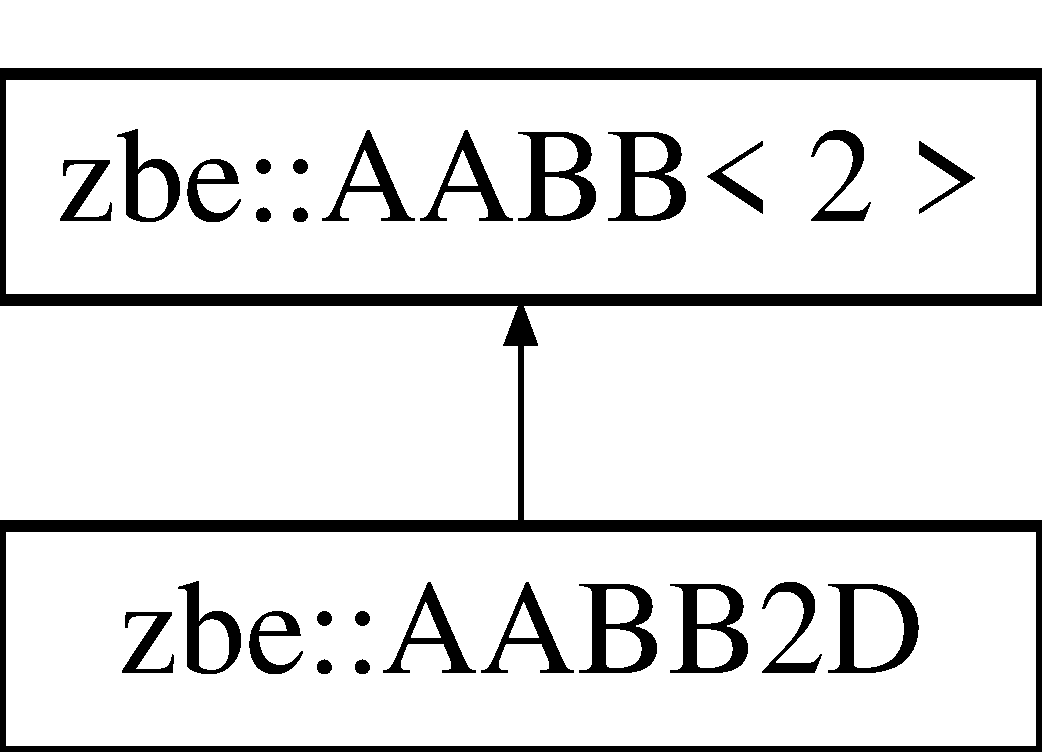
\includegraphics[height=2.000000cm]{structzbe_1_1_a_a_b_b2_d}
\end{center}
\end{figure}
\subsection*{Public Member Functions}
\begin{DoxyCompactItemize}
\item 
\hyperlink{structzbe_1_1_a_a_b_b2_d_a26a6ef5f3475f47bf4d92d6087a870ee}{A\+A\+B\+B2\+D} ()
\item 
\hyperlink{structzbe_1_1_a_a_b_b2_d_a07e6b3fc862c455a621c9743423c5ef2}{A\+A\+B\+B2\+D} (\hyperlink{classzbe_1_1_point}{Point}$<$ 2 $>$ pmin, \hyperlink{classzbe_1_1_point}{Point}$<$ 2 $>$ pmax)
\item 
\hyperlink{structzbe_1_1_a_a_b_b2_d_a5cc61bb61d08a3fc4f8100a6e7095084}{A\+A\+B\+B2\+D} (std\+::initializer\+\_\+list$<$ double $>$ lmin, std\+::initializer\+\_\+list$<$ double $>$ lmax)
\end{DoxyCompactItemize}
\subsection*{Additional Inherited Members}


\subsection{Detailed Description}


Definition at line 76 of file objects.\+h.



\subsection{Constructor \& Destructor Documentation}
\hypertarget{structzbe_1_1_a_a_b_b2_d_a26a6ef5f3475f47bf4d92d6087a870ee}{}\index{zbe\+::\+A\+A\+B\+B2\+D@{zbe\+::\+A\+A\+B\+B2\+D}!A\+A\+B\+B2\+D@{A\+A\+B\+B2\+D}}
\index{A\+A\+B\+B2\+D@{A\+A\+B\+B2\+D}!zbe\+::\+A\+A\+B\+B2\+D@{zbe\+::\+A\+A\+B\+B2\+D}}
\subsubsection[{A\+A\+B\+B2\+D()}]{\setlength{\rightskip}{0pt plus 5cm}zbe\+::\+A\+A\+B\+B2\+D\+::\+A\+A\+B\+B2\+D (
\begin{DoxyParamCaption}
{}
\end{DoxyParamCaption}
)\hspace{0.3cm}{\ttfamily [inline]}}\label{structzbe_1_1_a_a_b_b2_d_a26a6ef5f3475f47bf4d92d6087a870ee}


Definition at line 77 of file objects.\+h.

\hypertarget{structzbe_1_1_a_a_b_b2_d_a07e6b3fc862c455a621c9743423c5ef2}{}\index{zbe\+::\+A\+A\+B\+B2\+D@{zbe\+::\+A\+A\+B\+B2\+D}!A\+A\+B\+B2\+D@{A\+A\+B\+B2\+D}}
\index{A\+A\+B\+B2\+D@{A\+A\+B\+B2\+D}!zbe\+::\+A\+A\+B\+B2\+D@{zbe\+::\+A\+A\+B\+B2\+D}}
\subsubsection[{A\+A\+B\+B2\+D(\+Point$<$ 2 $>$ pmin, Point$<$ 2 $>$ pmax)}]{\setlength{\rightskip}{0pt plus 5cm}zbe\+::\+A\+A\+B\+B2\+D\+::\+A\+A\+B\+B2\+D (
\begin{DoxyParamCaption}
\item[{{\bf Point}$<$ 2 $>$}]{pmin, }
\item[{{\bf Point}$<$ 2 $>$}]{pmax}
\end{DoxyParamCaption}
)\hspace{0.3cm}{\ttfamily [inline]}}\label{structzbe_1_1_a_a_b_b2_d_a07e6b3fc862c455a621c9743423c5ef2}


Definition at line 78 of file objects.\+h.

\hypertarget{structzbe_1_1_a_a_b_b2_d_a5cc61bb61d08a3fc4f8100a6e7095084}{}\index{zbe\+::\+A\+A\+B\+B2\+D@{zbe\+::\+A\+A\+B\+B2\+D}!A\+A\+B\+B2\+D@{A\+A\+B\+B2\+D}}
\index{A\+A\+B\+B2\+D@{A\+A\+B\+B2\+D}!zbe\+::\+A\+A\+B\+B2\+D@{zbe\+::\+A\+A\+B\+B2\+D}}
\subsubsection[{A\+A\+B\+B2\+D(std\+::initializer\+\_\+list$<$ double $>$ lmin, std\+::initializer\+\_\+list$<$ double $>$ lmax)}]{\setlength{\rightskip}{0pt plus 5cm}zbe\+::\+A\+A\+B\+B2\+D\+::\+A\+A\+B\+B2\+D (
\begin{DoxyParamCaption}
\item[{std\+::initializer\+\_\+list$<$ double $>$}]{lmin, }
\item[{std\+::initializer\+\_\+list$<$ double $>$}]{lmax}
\end{DoxyParamCaption}
)\hspace{0.3cm}{\ttfamily [inline]}}\label{structzbe_1_1_a_a_b_b2_d_a5cc61bb61d08a3fc4f8100a6e7095084}


Definition at line 79 of file objects.\+h.



The documentation for this struct was generated from the following file\+:\begin{DoxyCompactItemize}
\item 
include/\+Z\+B\+E/core/tools/math/\hyperlink{objects_8h}{objects.\+h}\end{DoxyCompactItemize}

\hypertarget{structzbe_1_1_a_a_b_b3_d}{}\section{zbe\+:\+:A\+A\+B\+B3\+D Struct Reference}
\label{structzbe_1_1_a_a_b_b3_d}\index{zbe\+::\+A\+A\+B\+B3\+D@{zbe\+::\+A\+A\+B\+B3\+D}}


{\ttfamily \#include $<$objects.\+h$>$}

Inheritance diagram for zbe\+:\+:A\+A\+B\+B3\+D\+:\begin{figure}[H]
\begin{center}
\leavevmode
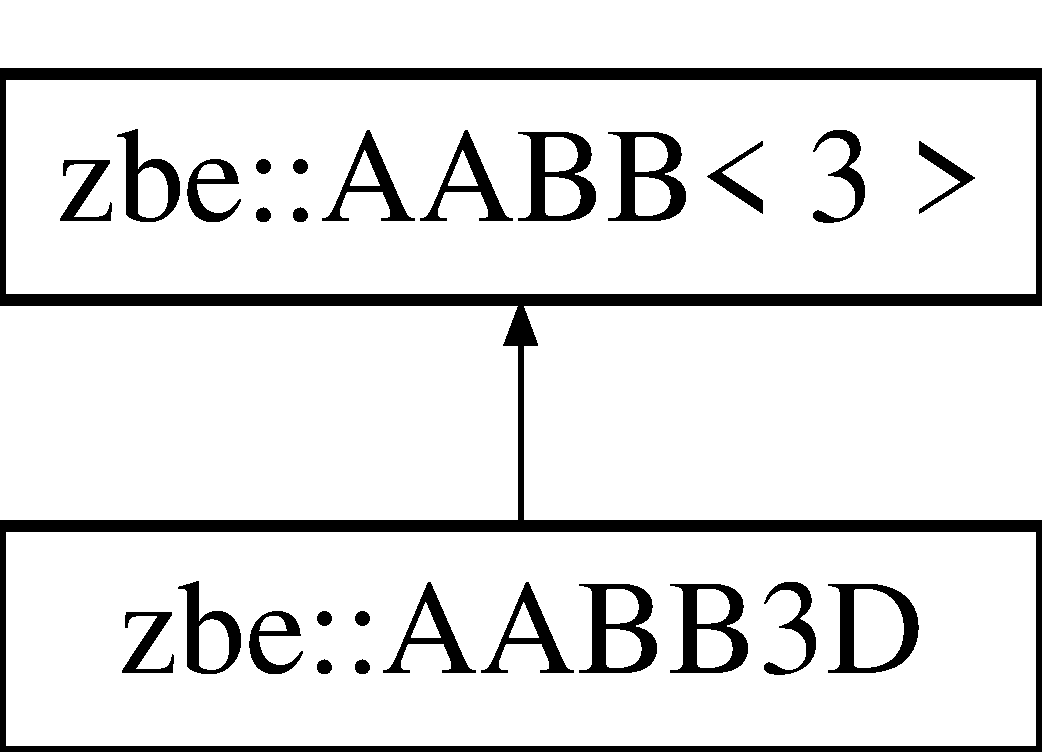
\includegraphics[height=2.000000cm]{structzbe_1_1_a_a_b_b3_d}
\end{center}
\end{figure}
\subsection*{Public Member Functions}
\begin{DoxyCompactItemize}
\item 
\hyperlink{structzbe_1_1_a_a_b_b3_d_a1ebf6148bbf48402f7646bb9a15b3669}{A\+A\+B\+B3\+D} ()
\item 
\hyperlink{structzbe_1_1_a_a_b_b3_d_a18340286ab0e01f06db7b181291b4ce0}{A\+A\+B\+B3\+D} (\hyperlink{classzbe_1_1_point}{Point}$<$ 3 $>$ pmin, \hyperlink{classzbe_1_1_point}{Point}$<$ 3 $>$ pmax)
\item 
\hyperlink{structzbe_1_1_a_a_b_b3_d_ab752e4a199de0f88944285acc9b3d878}{A\+A\+B\+B3\+D} (std\+::initializer\+\_\+list$<$ double $>$ lmin, std\+::initializer\+\_\+list$<$ double $>$ lmax)
\end{DoxyCompactItemize}
\subsection*{Additional Inherited Members}


\subsection{Detailed Description}


Definition at line 82 of file objects.\+h.



\subsection{Constructor \& Destructor Documentation}
\hypertarget{structzbe_1_1_a_a_b_b3_d_a1ebf6148bbf48402f7646bb9a15b3669}{}\index{zbe\+::\+A\+A\+B\+B3\+D@{zbe\+::\+A\+A\+B\+B3\+D}!A\+A\+B\+B3\+D@{A\+A\+B\+B3\+D}}
\index{A\+A\+B\+B3\+D@{A\+A\+B\+B3\+D}!zbe\+::\+A\+A\+B\+B3\+D@{zbe\+::\+A\+A\+B\+B3\+D}}
\subsubsection[{A\+A\+B\+B3\+D()}]{\setlength{\rightskip}{0pt plus 5cm}zbe\+::\+A\+A\+B\+B3\+D\+::\+A\+A\+B\+B3\+D (
\begin{DoxyParamCaption}
{}
\end{DoxyParamCaption}
)\hspace{0.3cm}{\ttfamily [inline]}}\label{structzbe_1_1_a_a_b_b3_d_a1ebf6148bbf48402f7646bb9a15b3669}


Definition at line 83 of file objects.\+h.

\hypertarget{structzbe_1_1_a_a_b_b3_d_a18340286ab0e01f06db7b181291b4ce0}{}\index{zbe\+::\+A\+A\+B\+B3\+D@{zbe\+::\+A\+A\+B\+B3\+D}!A\+A\+B\+B3\+D@{A\+A\+B\+B3\+D}}
\index{A\+A\+B\+B3\+D@{A\+A\+B\+B3\+D}!zbe\+::\+A\+A\+B\+B3\+D@{zbe\+::\+A\+A\+B\+B3\+D}}
\subsubsection[{A\+A\+B\+B3\+D(\+Point$<$ 3 $>$ pmin, Point$<$ 3 $>$ pmax)}]{\setlength{\rightskip}{0pt plus 5cm}zbe\+::\+A\+A\+B\+B3\+D\+::\+A\+A\+B\+B3\+D (
\begin{DoxyParamCaption}
\item[{{\bf Point}$<$ 3 $>$}]{pmin, }
\item[{{\bf Point}$<$ 3 $>$}]{pmax}
\end{DoxyParamCaption}
)\hspace{0.3cm}{\ttfamily [inline]}}\label{structzbe_1_1_a_a_b_b3_d_a18340286ab0e01f06db7b181291b4ce0}


Definition at line 84 of file objects.\+h.

\hypertarget{structzbe_1_1_a_a_b_b3_d_ab752e4a199de0f88944285acc9b3d878}{}\index{zbe\+::\+A\+A\+B\+B3\+D@{zbe\+::\+A\+A\+B\+B3\+D}!A\+A\+B\+B3\+D@{A\+A\+B\+B3\+D}}
\index{A\+A\+B\+B3\+D@{A\+A\+B\+B3\+D}!zbe\+::\+A\+A\+B\+B3\+D@{zbe\+::\+A\+A\+B\+B3\+D}}
\subsubsection[{A\+A\+B\+B3\+D(std\+::initializer\+\_\+list$<$ double $>$ lmin, std\+::initializer\+\_\+list$<$ double $>$ lmax)}]{\setlength{\rightskip}{0pt plus 5cm}zbe\+::\+A\+A\+B\+B3\+D\+::\+A\+A\+B\+B3\+D (
\begin{DoxyParamCaption}
\item[{std\+::initializer\+\_\+list$<$ double $>$}]{lmin, }
\item[{std\+::initializer\+\_\+list$<$ double $>$}]{lmax}
\end{DoxyParamCaption}
)\hspace{0.3cm}{\ttfamily [inline]}}\label{structzbe_1_1_a_a_b_b3_d_ab752e4a199de0f88944285acc9b3d878}


Definition at line 85 of file objects.\+h.



The documentation for this struct was generated from the following file\+:\begin{DoxyCompactItemize}
\item 
include/\+Z\+B\+E/core/tools/math/\hyperlink{objects_8h}{objects.\+h}\end{DoxyCompactItemize}

\hypertarget{classzbe_1_1_a_a_b_b_collisionable}{}\section{zbe\+:\+:A\+A\+B\+B\+Collisionable Class Reference}
\label{classzbe_1_1_a_a_b_b_collisionable}\index{zbe\+::\+A\+A\+B\+B\+Collisionable@{zbe\+::\+A\+A\+B\+B\+Collisionable}}


{\ttfamily \#include $<$A\+A\+B\+B\+Collisionable.\+h$>$}

\subsection*{Public Member Functions}
\begin{DoxyCompactItemize}
\item 
\hyperlink{classzbe_1_1_a_a_b_b_collisionable_a2c618917a1305b1f1c3f133dd57f43eb}{A\+A\+B\+B\+Collisionable} ()
\item 
\hyperlink{classzbe_1_1_a_a_b_b_collisionable_aadebaf0722b4bd0e9749658f0c7c29bc}{A\+A\+B\+B\+Collisionable} (int x, int y, unsigned width, unsigned height, unsigned radius)
\item 
\hyperlink{classzbe_1_1_a_a_b_b_collisionable_a2bdc3582874cffcc4c0e9d0309a55d3c}{$\sim$\+A\+A\+B\+B\+Collisionable} ()
\item 
void \hyperlink{classzbe_1_1_a_a_b_b_collisionable_a09ce11d77821bef2b83f03f2ee35ee0e}{set\+X} (int x)
\item 
void \hyperlink{classzbe_1_1_a_a_b_b_collisionable_a27f67daba6fd935cb0b454801a6bbf2e}{set\+Y} (int y)
\item 
void \hyperlink{classzbe_1_1_a_a_b_b_collisionable_a36336aea2619b7de7a94d14cfc289ce3}{set\+Width} (unsigned width)
\item 
void \hyperlink{classzbe_1_1_a_a_b_b_collisionable_a323e9d9ac50c752e300b97570cc69fd6}{set\+Height} (unsigned height)
\item 
void \hyperlink{classzbe_1_1_a_a_b_b_collisionable_a8e7cc35084c4bea04ce93f5d35db736a}{set\+Radius} (unsigned radius)
\item 
int \hyperlink{classzbe_1_1_a_a_b_b_collisionable_acca6f2333b2c225945c87862866e5163}{get\+X} () const 
\item 
int \hyperlink{classzbe_1_1_a_a_b_b_collisionable_a9ecee81fbd576f86a2480876e9bb226d}{get\+Y} () const 
\item 
unsigned \hyperlink{classzbe_1_1_a_a_b_b_collisionable_add5a7671229494a0668e14e0249ffa46}{get\+Width} () const 
\item 
unsigned \hyperlink{classzbe_1_1_a_a_b_b_collisionable_a734efe0e0654be4a9c319d5f22992dba}{get\+Height} () const 
\item 
unsigned \hyperlink{classzbe_1_1_a_a_b_b_collisionable_ae6db8c180e3dc9e9323f2c6c7803a87c}{get\+Radius} () const 
\end{DoxyCompactItemize}


\subsection{Detailed Description}


Definition at line 15 of file A\+A\+B\+B\+Collisionable.\+h.



\subsection{Constructor \& Destructor Documentation}
\hypertarget{classzbe_1_1_a_a_b_b_collisionable_a2c618917a1305b1f1c3f133dd57f43eb}{}\index{zbe\+::\+A\+A\+B\+B\+Collisionable@{zbe\+::\+A\+A\+B\+B\+Collisionable}!A\+A\+B\+B\+Collisionable@{A\+A\+B\+B\+Collisionable}}
\index{A\+A\+B\+B\+Collisionable@{A\+A\+B\+B\+Collisionable}!zbe\+::\+A\+A\+B\+B\+Collisionable@{zbe\+::\+A\+A\+B\+B\+Collisionable}}
\subsubsection[{A\+A\+B\+B\+Collisionable()}]{\setlength{\rightskip}{0pt plus 5cm}zbe\+::\+A\+A\+B\+B\+Collisionable\+::\+A\+A\+B\+B\+Collisionable (
\begin{DoxyParamCaption}
{}
\end{DoxyParamCaption}
)\hspace{0.3cm}{\ttfamily [inline]}}\label{classzbe_1_1_a_a_b_b_collisionable_a2c618917a1305b1f1c3f133dd57f43eb}


Definition at line 17 of file A\+A\+B\+B\+Collisionable.\+h.

\hypertarget{classzbe_1_1_a_a_b_b_collisionable_aadebaf0722b4bd0e9749658f0c7c29bc}{}\index{zbe\+::\+A\+A\+B\+B\+Collisionable@{zbe\+::\+A\+A\+B\+B\+Collisionable}!A\+A\+B\+B\+Collisionable@{A\+A\+B\+B\+Collisionable}}
\index{A\+A\+B\+B\+Collisionable@{A\+A\+B\+B\+Collisionable}!zbe\+::\+A\+A\+B\+B\+Collisionable@{zbe\+::\+A\+A\+B\+B\+Collisionable}}
\subsubsection[{A\+A\+B\+B\+Collisionable(int x, int y, unsigned width, unsigned height, unsigned radius)}]{\setlength{\rightskip}{0pt plus 5cm}zbe\+::\+A\+A\+B\+B\+Collisionable\+::\+A\+A\+B\+B\+Collisionable (
\begin{DoxyParamCaption}
\item[{int}]{x, }
\item[{int}]{y, }
\item[{unsigned}]{width, }
\item[{unsigned}]{height, }
\item[{unsigned}]{radius}
\end{DoxyParamCaption}
)\hspace{0.3cm}{\ttfamily [inline]}}\label{classzbe_1_1_a_a_b_b_collisionable_aadebaf0722b4bd0e9749658f0c7c29bc}


Definition at line 18 of file A\+A\+B\+B\+Collisionable.\+h.

\hypertarget{classzbe_1_1_a_a_b_b_collisionable_a2bdc3582874cffcc4c0e9d0309a55d3c}{}\index{zbe\+::\+A\+A\+B\+B\+Collisionable@{zbe\+::\+A\+A\+B\+B\+Collisionable}!````~A\+A\+B\+B\+Collisionable@{$\sim$\+A\+A\+B\+B\+Collisionable}}
\index{````~A\+A\+B\+B\+Collisionable@{$\sim$\+A\+A\+B\+B\+Collisionable}!zbe\+::\+A\+A\+B\+B\+Collisionable@{zbe\+::\+A\+A\+B\+B\+Collisionable}}
\subsubsection[{$\sim$\+A\+A\+B\+B\+Collisionable()}]{\setlength{\rightskip}{0pt plus 5cm}zbe\+::\+A\+A\+B\+B\+Collisionable\+::$\sim$\+A\+A\+B\+B\+Collisionable (
\begin{DoxyParamCaption}
{}
\end{DoxyParamCaption}
)\hspace{0.3cm}{\ttfamily [inline]}}\label{classzbe_1_1_a_a_b_b_collisionable_a2bdc3582874cffcc4c0e9d0309a55d3c}


Definition at line 20 of file A\+A\+B\+B\+Collisionable.\+h.



\subsection{Member Function Documentation}
\hypertarget{classzbe_1_1_a_a_b_b_collisionable_a734efe0e0654be4a9c319d5f22992dba}{}\index{zbe\+::\+A\+A\+B\+B\+Collisionable@{zbe\+::\+A\+A\+B\+B\+Collisionable}!get\+Height@{get\+Height}}
\index{get\+Height@{get\+Height}!zbe\+::\+A\+A\+B\+B\+Collisionable@{zbe\+::\+A\+A\+B\+B\+Collisionable}}
\subsubsection[{get\+Height() const }]{\setlength{\rightskip}{0pt plus 5cm}unsigned zbe\+::\+A\+A\+B\+B\+Collisionable\+::get\+Height (
\begin{DoxyParamCaption}
{}
\end{DoxyParamCaption}
) const\hspace{0.3cm}{\ttfamily [inline]}}\label{classzbe_1_1_a_a_b_b_collisionable_a734efe0e0654be4a9c319d5f22992dba}


Definition at line 31 of file A\+A\+B\+B\+Collisionable.\+h.

\hypertarget{classzbe_1_1_a_a_b_b_collisionable_ae6db8c180e3dc9e9323f2c6c7803a87c}{}\index{zbe\+::\+A\+A\+B\+B\+Collisionable@{zbe\+::\+A\+A\+B\+B\+Collisionable}!get\+Radius@{get\+Radius}}
\index{get\+Radius@{get\+Radius}!zbe\+::\+A\+A\+B\+B\+Collisionable@{zbe\+::\+A\+A\+B\+B\+Collisionable}}
\subsubsection[{get\+Radius() const }]{\setlength{\rightskip}{0pt plus 5cm}unsigned zbe\+::\+A\+A\+B\+B\+Collisionable\+::get\+Radius (
\begin{DoxyParamCaption}
{}
\end{DoxyParamCaption}
) const\hspace{0.3cm}{\ttfamily [inline]}}\label{classzbe_1_1_a_a_b_b_collisionable_ae6db8c180e3dc9e9323f2c6c7803a87c}


Definition at line 32 of file A\+A\+B\+B\+Collisionable.\+h.

\hypertarget{classzbe_1_1_a_a_b_b_collisionable_add5a7671229494a0668e14e0249ffa46}{}\index{zbe\+::\+A\+A\+B\+B\+Collisionable@{zbe\+::\+A\+A\+B\+B\+Collisionable}!get\+Width@{get\+Width}}
\index{get\+Width@{get\+Width}!zbe\+::\+A\+A\+B\+B\+Collisionable@{zbe\+::\+A\+A\+B\+B\+Collisionable}}
\subsubsection[{get\+Width() const }]{\setlength{\rightskip}{0pt plus 5cm}unsigned zbe\+::\+A\+A\+B\+B\+Collisionable\+::get\+Width (
\begin{DoxyParamCaption}
{}
\end{DoxyParamCaption}
) const\hspace{0.3cm}{\ttfamily [inline]}}\label{classzbe_1_1_a_a_b_b_collisionable_add5a7671229494a0668e14e0249ffa46}


Definition at line 30 of file A\+A\+B\+B\+Collisionable.\+h.

\hypertarget{classzbe_1_1_a_a_b_b_collisionable_acca6f2333b2c225945c87862866e5163}{}\index{zbe\+::\+A\+A\+B\+B\+Collisionable@{zbe\+::\+A\+A\+B\+B\+Collisionable}!get\+X@{get\+X}}
\index{get\+X@{get\+X}!zbe\+::\+A\+A\+B\+B\+Collisionable@{zbe\+::\+A\+A\+B\+B\+Collisionable}}
\subsubsection[{get\+X() const }]{\setlength{\rightskip}{0pt plus 5cm}int zbe\+::\+A\+A\+B\+B\+Collisionable\+::get\+X (
\begin{DoxyParamCaption}
{}
\end{DoxyParamCaption}
) const\hspace{0.3cm}{\ttfamily [inline]}}\label{classzbe_1_1_a_a_b_b_collisionable_acca6f2333b2c225945c87862866e5163}


Definition at line 28 of file A\+A\+B\+B\+Collisionable.\+h.

\hypertarget{classzbe_1_1_a_a_b_b_collisionable_a9ecee81fbd576f86a2480876e9bb226d}{}\index{zbe\+::\+A\+A\+B\+B\+Collisionable@{zbe\+::\+A\+A\+B\+B\+Collisionable}!get\+Y@{get\+Y}}
\index{get\+Y@{get\+Y}!zbe\+::\+A\+A\+B\+B\+Collisionable@{zbe\+::\+A\+A\+B\+B\+Collisionable}}
\subsubsection[{get\+Y() const }]{\setlength{\rightskip}{0pt plus 5cm}int zbe\+::\+A\+A\+B\+B\+Collisionable\+::get\+Y (
\begin{DoxyParamCaption}
{}
\end{DoxyParamCaption}
) const\hspace{0.3cm}{\ttfamily [inline]}}\label{classzbe_1_1_a_a_b_b_collisionable_a9ecee81fbd576f86a2480876e9bb226d}


Definition at line 29 of file A\+A\+B\+B\+Collisionable.\+h.

\hypertarget{classzbe_1_1_a_a_b_b_collisionable_a323e9d9ac50c752e300b97570cc69fd6}{}\index{zbe\+::\+A\+A\+B\+B\+Collisionable@{zbe\+::\+A\+A\+B\+B\+Collisionable}!set\+Height@{set\+Height}}
\index{set\+Height@{set\+Height}!zbe\+::\+A\+A\+B\+B\+Collisionable@{zbe\+::\+A\+A\+B\+B\+Collisionable}}
\subsubsection[{set\+Height(unsigned height)}]{\setlength{\rightskip}{0pt plus 5cm}void zbe\+::\+A\+A\+B\+B\+Collisionable\+::set\+Height (
\begin{DoxyParamCaption}
\item[{unsigned}]{height}
\end{DoxyParamCaption}
)\hspace{0.3cm}{\ttfamily [inline]}}\label{classzbe_1_1_a_a_b_b_collisionable_a323e9d9ac50c752e300b97570cc69fd6}


Definition at line 25 of file A\+A\+B\+B\+Collisionable.\+h.

\hypertarget{classzbe_1_1_a_a_b_b_collisionable_a8e7cc35084c4bea04ce93f5d35db736a}{}\index{zbe\+::\+A\+A\+B\+B\+Collisionable@{zbe\+::\+A\+A\+B\+B\+Collisionable}!set\+Radius@{set\+Radius}}
\index{set\+Radius@{set\+Radius}!zbe\+::\+A\+A\+B\+B\+Collisionable@{zbe\+::\+A\+A\+B\+B\+Collisionable}}
\subsubsection[{set\+Radius(unsigned radius)}]{\setlength{\rightskip}{0pt plus 5cm}void zbe\+::\+A\+A\+B\+B\+Collisionable\+::set\+Radius (
\begin{DoxyParamCaption}
\item[{unsigned}]{radius}
\end{DoxyParamCaption}
)\hspace{0.3cm}{\ttfamily [inline]}}\label{classzbe_1_1_a_a_b_b_collisionable_a8e7cc35084c4bea04ce93f5d35db736a}


Definition at line 26 of file A\+A\+B\+B\+Collisionable.\+h.

\hypertarget{classzbe_1_1_a_a_b_b_collisionable_a36336aea2619b7de7a94d14cfc289ce3}{}\index{zbe\+::\+A\+A\+B\+B\+Collisionable@{zbe\+::\+A\+A\+B\+B\+Collisionable}!set\+Width@{set\+Width}}
\index{set\+Width@{set\+Width}!zbe\+::\+A\+A\+B\+B\+Collisionable@{zbe\+::\+A\+A\+B\+B\+Collisionable}}
\subsubsection[{set\+Width(unsigned width)}]{\setlength{\rightskip}{0pt plus 5cm}void zbe\+::\+A\+A\+B\+B\+Collisionable\+::set\+Width (
\begin{DoxyParamCaption}
\item[{unsigned}]{width}
\end{DoxyParamCaption}
)\hspace{0.3cm}{\ttfamily [inline]}}\label{classzbe_1_1_a_a_b_b_collisionable_a36336aea2619b7de7a94d14cfc289ce3}


Definition at line 24 of file A\+A\+B\+B\+Collisionable.\+h.

\hypertarget{classzbe_1_1_a_a_b_b_collisionable_a09ce11d77821bef2b83f03f2ee35ee0e}{}\index{zbe\+::\+A\+A\+B\+B\+Collisionable@{zbe\+::\+A\+A\+B\+B\+Collisionable}!set\+X@{set\+X}}
\index{set\+X@{set\+X}!zbe\+::\+A\+A\+B\+B\+Collisionable@{zbe\+::\+A\+A\+B\+B\+Collisionable}}
\subsubsection[{set\+X(int x)}]{\setlength{\rightskip}{0pt plus 5cm}void zbe\+::\+A\+A\+B\+B\+Collisionable\+::set\+X (
\begin{DoxyParamCaption}
\item[{int}]{x}
\end{DoxyParamCaption}
)\hspace{0.3cm}{\ttfamily [inline]}}\label{classzbe_1_1_a_a_b_b_collisionable_a09ce11d77821bef2b83f03f2ee35ee0e}


Definition at line 22 of file A\+A\+B\+B\+Collisionable.\+h.

\hypertarget{classzbe_1_1_a_a_b_b_collisionable_a27f67daba6fd935cb0b454801a6bbf2e}{}\index{zbe\+::\+A\+A\+B\+B\+Collisionable@{zbe\+::\+A\+A\+B\+B\+Collisionable}!set\+Y@{set\+Y}}
\index{set\+Y@{set\+Y}!zbe\+::\+A\+A\+B\+B\+Collisionable@{zbe\+::\+A\+A\+B\+B\+Collisionable}}
\subsubsection[{set\+Y(int y)}]{\setlength{\rightskip}{0pt plus 5cm}void zbe\+::\+A\+A\+B\+B\+Collisionable\+::set\+Y (
\begin{DoxyParamCaption}
\item[{int}]{y}
\end{DoxyParamCaption}
)\hspace{0.3cm}{\ttfamily [inline]}}\label{classzbe_1_1_a_a_b_b_collisionable_a27f67daba6fd935cb0b454801a6bbf2e}


Definition at line 23 of file A\+A\+B\+B\+Collisionable.\+h.



The documentation for this class was generated from the following file\+:\begin{DoxyCompactItemize}
\item 
include/\+Z\+B\+E/core/archetypes/\hyperlink{_a_a_b_b_collisionable_8h}{A\+A\+B\+B\+Collisionable.\+h}\end{DoxyCompactItemize}

\hypertarget{classzbe_1_1_a_a_b_b_sphere_collisionable}{}\section{zbe\+:\+:A\+A\+B\+B\+Sphere\+Collisionable Class Reference}
\label{classzbe_1_1_a_a_b_b_sphere_collisionable}\index{zbe\+::\+A\+A\+B\+B\+Sphere\+Collisionable@{zbe\+::\+A\+A\+B\+B\+Sphere\+Collisionable}}


{\ttfamily \#include $<$A\+A\+B\+B\+Sphere\+Collisionable.\+h$>$}

\subsection*{Public Member Functions}
\begin{DoxyCompactItemize}
\item 
\hyperlink{classzbe_1_1_a_a_b_b_sphere_collisionable_a981bd06ba88c73b3cb905eea09d3c669}{A\+A\+B\+B\+Sphere\+Collisionable} ()
\item 
\hyperlink{classzbe_1_1_a_a_b_b_sphere_collisionable_a9dfd2b1b3db7ef47d5dafc3ec0c30d5a}{A\+A\+B\+B\+Sphere\+Collisionable} (int x, int y, unsigned width, unsigned height, unsigned radius)
\item 
\hyperlink{classzbe_1_1_a_a_b_b_sphere_collisionable_a63703824de5c12015f674e8e1b7cd01d}{$\sim$\+A\+A\+B\+B\+Sphere\+Collisionable} ()
\item 
void \hyperlink{classzbe_1_1_a_a_b_b_sphere_collisionable_a11d7e44875717dc713f00513a0d2ee9c}{set\+X} (int x)
\item 
void \hyperlink{classzbe_1_1_a_a_b_b_sphere_collisionable_a1a40956e0431b5ddb0763f8676e23465}{set\+Y} (int y)
\item 
void \hyperlink{classzbe_1_1_a_a_b_b_sphere_collisionable_a0f508e2f634c907d6dcbc5a3472fea54}{set\+Width} (unsigned width)
\item 
void \hyperlink{classzbe_1_1_a_a_b_b_sphere_collisionable_a996e8f134bd9ce3f22932cf5b010ec6d}{set\+Height} (unsigned height)
\item 
void \hyperlink{classzbe_1_1_a_a_b_b_sphere_collisionable_a5fb8c95e108ae3ecd5eb66f75a0ebb62}{set\+Radius} (unsigned radius)
\item 
int \hyperlink{classzbe_1_1_a_a_b_b_sphere_collisionable_abafe7ff2a79f52e41b7022a8fcda305f}{get\+X} () const 
\item 
int \hyperlink{classzbe_1_1_a_a_b_b_sphere_collisionable_a13c4e3749adba1048f36b4660a188da6}{get\+Y} () const 
\item 
unsigned \hyperlink{classzbe_1_1_a_a_b_b_sphere_collisionable_ad92f187845cfd459ee560a0a93fbbeea}{get\+Width} () const 
\item 
unsigned \hyperlink{classzbe_1_1_a_a_b_b_sphere_collisionable_ade399f9d6e9f1d5dd28bc8bd1c9b1be2}{get\+Height} () const 
\item 
unsigned \hyperlink{classzbe_1_1_a_a_b_b_sphere_collisionable_a5dc34b230c3f7fe312bb4e2bede3a38a}{get\+Radius} () const 
\end{DoxyCompactItemize}


\subsection{Detailed Description}


Definition at line 23 of file A\+A\+B\+B\+Sphere\+Collisionable.\+h.



\subsection{Constructor \& Destructor Documentation}
\hypertarget{classzbe_1_1_a_a_b_b_sphere_collisionable_a981bd06ba88c73b3cb905eea09d3c669}{}\index{zbe\+::\+A\+A\+B\+B\+Sphere\+Collisionable@{zbe\+::\+A\+A\+B\+B\+Sphere\+Collisionable}!A\+A\+B\+B\+Sphere\+Collisionable@{A\+A\+B\+B\+Sphere\+Collisionable}}
\index{A\+A\+B\+B\+Sphere\+Collisionable@{A\+A\+B\+B\+Sphere\+Collisionable}!zbe\+::\+A\+A\+B\+B\+Sphere\+Collisionable@{zbe\+::\+A\+A\+B\+B\+Sphere\+Collisionable}}
\subsubsection[{A\+A\+B\+B\+Sphere\+Collisionable()}]{\setlength{\rightskip}{0pt plus 5cm}zbe\+::\+A\+A\+B\+B\+Sphere\+Collisionable\+::\+A\+A\+B\+B\+Sphere\+Collisionable (
\begin{DoxyParamCaption}
{}
\end{DoxyParamCaption}
)\hspace{0.3cm}{\ttfamily [inline]}}\label{classzbe_1_1_a_a_b_b_sphere_collisionable_a981bd06ba88c73b3cb905eea09d3c669}


Definition at line 25 of file A\+A\+B\+B\+Sphere\+Collisionable.\+h.

\hypertarget{classzbe_1_1_a_a_b_b_sphere_collisionable_a9dfd2b1b3db7ef47d5dafc3ec0c30d5a}{}\index{zbe\+::\+A\+A\+B\+B\+Sphere\+Collisionable@{zbe\+::\+A\+A\+B\+B\+Sphere\+Collisionable}!A\+A\+B\+B\+Sphere\+Collisionable@{A\+A\+B\+B\+Sphere\+Collisionable}}
\index{A\+A\+B\+B\+Sphere\+Collisionable@{A\+A\+B\+B\+Sphere\+Collisionable}!zbe\+::\+A\+A\+B\+B\+Sphere\+Collisionable@{zbe\+::\+A\+A\+B\+B\+Sphere\+Collisionable}}
\subsubsection[{A\+A\+B\+B\+Sphere\+Collisionable(int x, int y, unsigned width, unsigned height, unsigned radius)}]{\setlength{\rightskip}{0pt plus 5cm}zbe\+::\+A\+A\+B\+B\+Sphere\+Collisionable\+::\+A\+A\+B\+B\+Sphere\+Collisionable (
\begin{DoxyParamCaption}
\item[{int}]{x, }
\item[{int}]{y, }
\item[{unsigned}]{width, }
\item[{unsigned}]{height, }
\item[{unsigned}]{radius}
\end{DoxyParamCaption}
)\hspace{0.3cm}{\ttfamily [inline]}}\label{classzbe_1_1_a_a_b_b_sphere_collisionable_a9dfd2b1b3db7ef47d5dafc3ec0c30d5a}


Definition at line 26 of file A\+A\+B\+B\+Sphere\+Collisionable.\+h.

\hypertarget{classzbe_1_1_a_a_b_b_sphere_collisionable_a63703824de5c12015f674e8e1b7cd01d}{}\index{zbe\+::\+A\+A\+B\+B\+Sphere\+Collisionable@{zbe\+::\+A\+A\+B\+B\+Sphere\+Collisionable}!````~A\+A\+B\+B\+Sphere\+Collisionable@{$\sim$\+A\+A\+B\+B\+Sphere\+Collisionable}}
\index{````~A\+A\+B\+B\+Sphere\+Collisionable@{$\sim$\+A\+A\+B\+B\+Sphere\+Collisionable}!zbe\+::\+A\+A\+B\+B\+Sphere\+Collisionable@{zbe\+::\+A\+A\+B\+B\+Sphere\+Collisionable}}
\subsubsection[{$\sim$\+A\+A\+B\+B\+Sphere\+Collisionable()}]{\setlength{\rightskip}{0pt plus 5cm}zbe\+::\+A\+A\+B\+B\+Sphere\+Collisionable\+::$\sim$\+A\+A\+B\+B\+Sphere\+Collisionable (
\begin{DoxyParamCaption}
{}
\end{DoxyParamCaption}
)\hspace{0.3cm}{\ttfamily [inline]}}\label{classzbe_1_1_a_a_b_b_sphere_collisionable_a63703824de5c12015f674e8e1b7cd01d}


Definition at line 28 of file A\+A\+B\+B\+Sphere\+Collisionable.\+h.



\subsection{Member Function Documentation}
\hypertarget{classzbe_1_1_a_a_b_b_sphere_collisionable_ade399f9d6e9f1d5dd28bc8bd1c9b1be2}{}\index{zbe\+::\+A\+A\+B\+B\+Sphere\+Collisionable@{zbe\+::\+A\+A\+B\+B\+Sphere\+Collisionable}!get\+Height@{get\+Height}}
\index{get\+Height@{get\+Height}!zbe\+::\+A\+A\+B\+B\+Sphere\+Collisionable@{zbe\+::\+A\+A\+B\+B\+Sphere\+Collisionable}}
\subsubsection[{get\+Height() const }]{\setlength{\rightskip}{0pt plus 5cm}unsigned zbe\+::\+A\+A\+B\+B\+Sphere\+Collisionable\+::get\+Height (
\begin{DoxyParamCaption}
{}
\end{DoxyParamCaption}
) const\hspace{0.3cm}{\ttfamily [inline]}}\label{classzbe_1_1_a_a_b_b_sphere_collisionable_ade399f9d6e9f1d5dd28bc8bd1c9b1be2}


Definition at line 39 of file A\+A\+B\+B\+Sphere\+Collisionable.\+h.

\hypertarget{classzbe_1_1_a_a_b_b_sphere_collisionable_a5dc34b230c3f7fe312bb4e2bede3a38a}{}\index{zbe\+::\+A\+A\+B\+B\+Sphere\+Collisionable@{zbe\+::\+A\+A\+B\+B\+Sphere\+Collisionable}!get\+Radius@{get\+Radius}}
\index{get\+Radius@{get\+Radius}!zbe\+::\+A\+A\+B\+B\+Sphere\+Collisionable@{zbe\+::\+A\+A\+B\+B\+Sphere\+Collisionable}}
\subsubsection[{get\+Radius() const }]{\setlength{\rightskip}{0pt plus 5cm}unsigned zbe\+::\+A\+A\+B\+B\+Sphere\+Collisionable\+::get\+Radius (
\begin{DoxyParamCaption}
{}
\end{DoxyParamCaption}
) const\hspace{0.3cm}{\ttfamily [inline]}}\label{classzbe_1_1_a_a_b_b_sphere_collisionable_a5dc34b230c3f7fe312bb4e2bede3a38a}


Definition at line 40 of file A\+A\+B\+B\+Sphere\+Collisionable.\+h.

\hypertarget{classzbe_1_1_a_a_b_b_sphere_collisionable_ad92f187845cfd459ee560a0a93fbbeea}{}\index{zbe\+::\+A\+A\+B\+B\+Sphere\+Collisionable@{zbe\+::\+A\+A\+B\+B\+Sphere\+Collisionable}!get\+Width@{get\+Width}}
\index{get\+Width@{get\+Width}!zbe\+::\+A\+A\+B\+B\+Sphere\+Collisionable@{zbe\+::\+A\+A\+B\+B\+Sphere\+Collisionable}}
\subsubsection[{get\+Width() const }]{\setlength{\rightskip}{0pt plus 5cm}unsigned zbe\+::\+A\+A\+B\+B\+Sphere\+Collisionable\+::get\+Width (
\begin{DoxyParamCaption}
{}
\end{DoxyParamCaption}
) const\hspace{0.3cm}{\ttfamily [inline]}}\label{classzbe_1_1_a_a_b_b_sphere_collisionable_ad92f187845cfd459ee560a0a93fbbeea}


Definition at line 38 of file A\+A\+B\+B\+Sphere\+Collisionable.\+h.

\hypertarget{classzbe_1_1_a_a_b_b_sphere_collisionable_abafe7ff2a79f52e41b7022a8fcda305f}{}\index{zbe\+::\+A\+A\+B\+B\+Sphere\+Collisionable@{zbe\+::\+A\+A\+B\+B\+Sphere\+Collisionable}!get\+X@{get\+X}}
\index{get\+X@{get\+X}!zbe\+::\+A\+A\+B\+B\+Sphere\+Collisionable@{zbe\+::\+A\+A\+B\+B\+Sphere\+Collisionable}}
\subsubsection[{get\+X() const }]{\setlength{\rightskip}{0pt plus 5cm}int zbe\+::\+A\+A\+B\+B\+Sphere\+Collisionable\+::get\+X (
\begin{DoxyParamCaption}
{}
\end{DoxyParamCaption}
) const\hspace{0.3cm}{\ttfamily [inline]}}\label{classzbe_1_1_a_a_b_b_sphere_collisionable_abafe7ff2a79f52e41b7022a8fcda305f}


Definition at line 36 of file A\+A\+B\+B\+Sphere\+Collisionable.\+h.

\hypertarget{classzbe_1_1_a_a_b_b_sphere_collisionable_a13c4e3749adba1048f36b4660a188da6}{}\index{zbe\+::\+A\+A\+B\+B\+Sphere\+Collisionable@{zbe\+::\+A\+A\+B\+B\+Sphere\+Collisionable}!get\+Y@{get\+Y}}
\index{get\+Y@{get\+Y}!zbe\+::\+A\+A\+B\+B\+Sphere\+Collisionable@{zbe\+::\+A\+A\+B\+B\+Sphere\+Collisionable}}
\subsubsection[{get\+Y() const }]{\setlength{\rightskip}{0pt plus 5cm}int zbe\+::\+A\+A\+B\+B\+Sphere\+Collisionable\+::get\+Y (
\begin{DoxyParamCaption}
{}
\end{DoxyParamCaption}
) const\hspace{0.3cm}{\ttfamily [inline]}}\label{classzbe_1_1_a_a_b_b_sphere_collisionable_a13c4e3749adba1048f36b4660a188da6}


Definition at line 37 of file A\+A\+B\+B\+Sphere\+Collisionable.\+h.

\hypertarget{classzbe_1_1_a_a_b_b_sphere_collisionable_a996e8f134bd9ce3f22932cf5b010ec6d}{}\index{zbe\+::\+A\+A\+B\+B\+Sphere\+Collisionable@{zbe\+::\+A\+A\+B\+B\+Sphere\+Collisionable}!set\+Height@{set\+Height}}
\index{set\+Height@{set\+Height}!zbe\+::\+A\+A\+B\+B\+Sphere\+Collisionable@{zbe\+::\+A\+A\+B\+B\+Sphere\+Collisionable}}
\subsubsection[{set\+Height(unsigned height)}]{\setlength{\rightskip}{0pt plus 5cm}void zbe\+::\+A\+A\+B\+B\+Sphere\+Collisionable\+::set\+Height (
\begin{DoxyParamCaption}
\item[{unsigned}]{height}
\end{DoxyParamCaption}
)\hspace{0.3cm}{\ttfamily [inline]}}\label{classzbe_1_1_a_a_b_b_sphere_collisionable_a996e8f134bd9ce3f22932cf5b010ec6d}


Definition at line 33 of file A\+A\+B\+B\+Sphere\+Collisionable.\+h.

\hypertarget{classzbe_1_1_a_a_b_b_sphere_collisionable_a5fb8c95e108ae3ecd5eb66f75a0ebb62}{}\index{zbe\+::\+A\+A\+B\+B\+Sphere\+Collisionable@{zbe\+::\+A\+A\+B\+B\+Sphere\+Collisionable}!set\+Radius@{set\+Radius}}
\index{set\+Radius@{set\+Radius}!zbe\+::\+A\+A\+B\+B\+Sphere\+Collisionable@{zbe\+::\+A\+A\+B\+B\+Sphere\+Collisionable}}
\subsubsection[{set\+Radius(unsigned radius)}]{\setlength{\rightskip}{0pt plus 5cm}void zbe\+::\+A\+A\+B\+B\+Sphere\+Collisionable\+::set\+Radius (
\begin{DoxyParamCaption}
\item[{unsigned}]{radius}
\end{DoxyParamCaption}
)\hspace{0.3cm}{\ttfamily [inline]}}\label{classzbe_1_1_a_a_b_b_sphere_collisionable_a5fb8c95e108ae3ecd5eb66f75a0ebb62}


Definition at line 34 of file A\+A\+B\+B\+Sphere\+Collisionable.\+h.

\hypertarget{classzbe_1_1_a_a_b_b_sphere_collisionable_a0f508e2f634c907d6dcbc5a3472fea54}{}\index{zbe\+::\+A\+A\+B\+B\+Sphere\+Collisionable@{zbe\+::\+A\+A\+B\+B\+Sphere\+Collisionable}!set\+Width@{set\+Width}}
\index{set\+Width@{set\+Width}!zbe\+::\+A\+A\+B\+B\+Sphere\+Collisionable@{zbe\+::\+A\+A\+B\+B\+Sphere\+Collisionable}}
\subsubsection[{set\+Width(unsigned width)}]{\setlength{\rightskip}{0pt plus 5cm}void zbe\+::\+A\+A\+B\+B\+Sphere\+Collisionable\+::set\+Width (
\begin{DoxyParamCaption}
\item[{unsigned}]{width}
\end{DoxyParamCaption}
)\hspace{0.3cm}{\ttfamily [inline]}}\label{classzbe_1_1_a_a_b_b_sphere_collisionable_a0f508e2f634c907d6dcbc5a3472fea54}


Definition at line 32 of file A\+A\+B\+B\+Sphere\+Collisionable.\+h.

\hypertarget{classzbe_1_1_a_a_b_b_sphere_collisionable_a11d7e44875717dc713f00513a0d2ee9c}{}\index{zbe\+::\+A\+A\+B\+B\+Sphere\+Collisionable@{zbe\+::\+A\+A\+B\+B\+Sphere\+Collisionable}!set\+X@{set\+X}}
\index{set\+X@{set\+X}!zbe\+::\+A\+A\+B\+B\+Sphere\+Collisionable@{zbe\+::\+A\+A\+B\+B\+Sphere\+Collisionable}}
\subsubsection[{set\+X(int x)}]{\setlength{\rightskip}{0pt plus 5cm}void zbe\+::\+A\+A\+B\+B\+Sphere\+Collisionable\+::set\+X (
\begin{DoxyParamCaption}
\item[{int}]{x}
\end{DoxyParamCaption}
)\hspace{0.3cm}{\ttfamily [inline]}}\label{classzbe_1_1_a_a_b_b_sphere_collisionable_a11d7e44875717dc713f00513a0d2ee9c}


Definition at line 30 of file A\+A\+B\+B\+Sphere\+Collisionable.\+h.

\hypertarget{classzbe_1_1_a_a_b_b_sphere_collisionable_a1a40956e0431b5ddb0763f8676e23465}{}\index{zbe\+::\+A\+A\+B\+B\+Sphere\+Collisionable@{zbe\+::\+A\+A\+B\+B\+Sphere\+Collisionable}!set\+Y@{set\+Y}}
\index{set\+Y@{set\+Y}!zbe\+::\+A\+A\+B\+B\+Sphere\+Collisionable@{zbe\+::\+A\+A\+B\+B\+Sphere\+Collisionable}}
\subsubsection[{set\+Y(int y)}]{\setlength{\rightskip}{0pt plus 5cm}void zbe\+::\+A\+A\+B\+B\+Sphere\+Collisionable\+::set\+Y (
\begin{DoxyParamCaption}
\item[{int}]{y}
\end{DoxyParamCaption}
)\hspace{0.3cm}{\ttfamily [inline]}}\label{classzbe_1_1_a_a_b_b_sphere_collisionable_a1a40956e0431b5ddb0763f8676e23465}


Definition at line 31 of file A\+A\+B\+B\+Sphere\+Collisionable.\+h.



The documentation for this class was generated from the following file\+:\begin{DoxyCompactItemize}
\item 
include/\+Z\+B\+E/core/archetypes/\hyperlink{_a_a_b_b_sphere_collisionable_8h}{A\+A\+B\+B\+Sphere\+Collisionable.\+h}\end{DoxyCompactItemize}

\hypertarget{classzbe_1_1_app}{}\section{zbe\+:\+:App Class Reference}
\label{classzbe_1_1_app}\index{zbe\+::\+App@{zbe\+::\+App}}


{\ttfamily \#include $<$App.\+h$>$}

Inheritance diagram for zbe\+:\+:App\+:\begin{figure}[H]
\begin{center}
\leavevmode
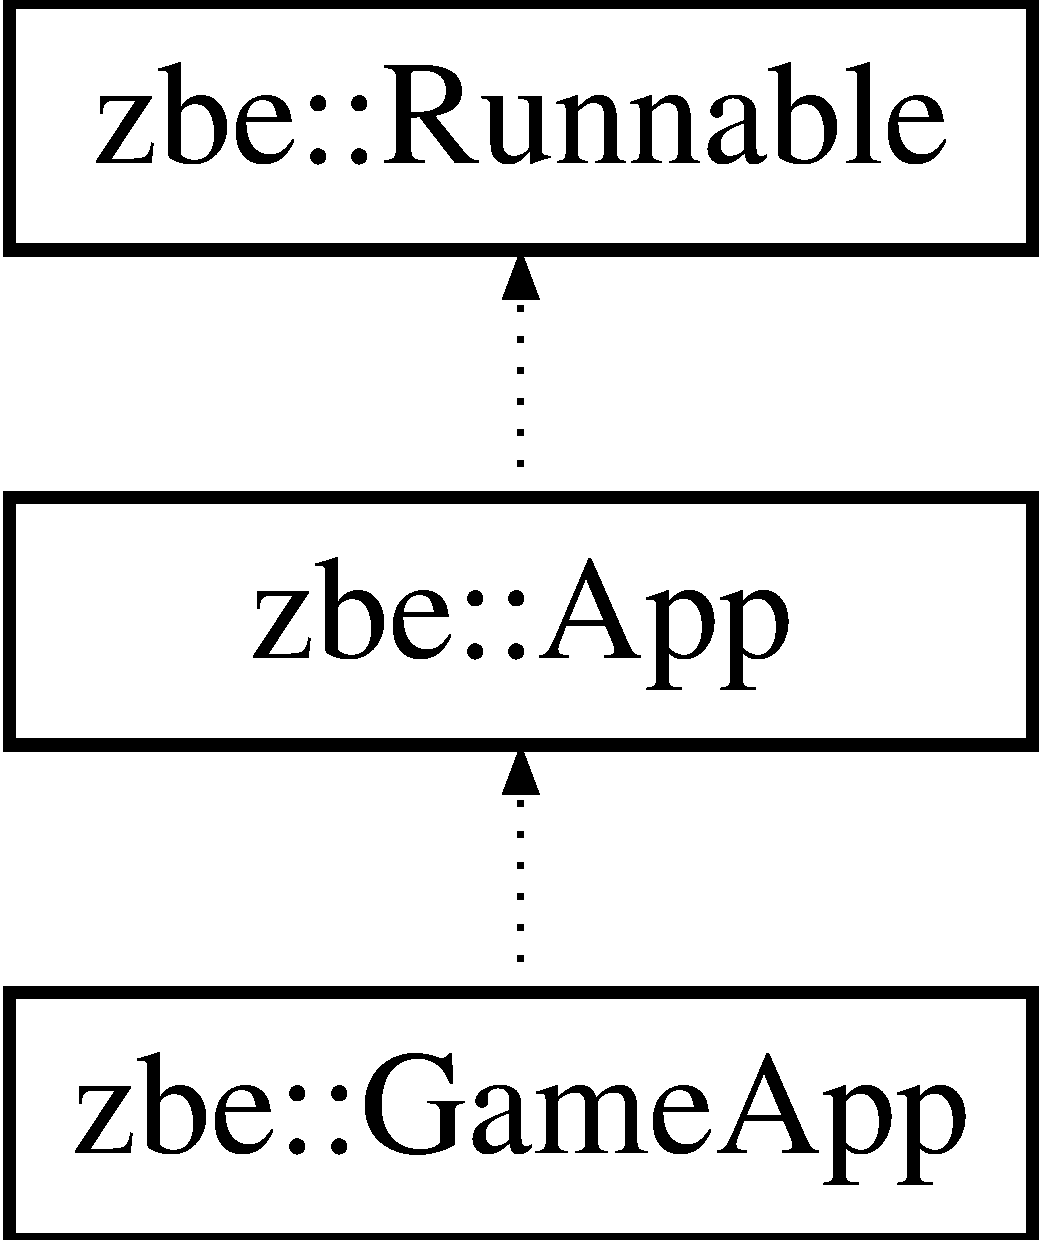
\includegraphics[height=3.000000cm]{classzbe_1_1_app}
\end{center}
\end{figure}
\subsection*{Public Member Functions}
\begin{DoxyCompactItemize}
\item 
virtual \hyperlink{classzbe_1_1_app_aabadd61b8978ed76690b89a3990389bc}{$\sim$\+App} ()
\item 
virtual void \hyperlink{classzbe_1_1_app_aa011954db631225be8e26af69ce3f21d}{setup} ()
\item 
virtual void \hyperlink{classzbe_1_1_app_ac66aa5f4083b6c2c11bbbe9dccde4b3b}{app} ()=0
\item 
virtual void \hyperlink{classzbe_1_1_app_a11ecb4eb1dddde6e7450ac5d3f37a78c}{shutdown} ()
\item 
void \hyperlink{classzbe_1_1_app_ac952b75e2efcf5c2967da60dd95b57e6}{run} ()
\item 
virtual void \hyperlink{classzbe_1_1_app_a4d4f1df38c315ff983c9be55b9e81ea3}{pause} ()
\item 
virtual void \hyperlink{classzbe_1_1_app_ae594070a4566ce4bee010be64b8ff24d}{resume} ()
\item 
virtual void \hyperlink{classzbe_1_1_app_acc49c52714ffe0aff04b3252225cceec}{restart} ()
\end{DoxyCompactItemize}


\subsection{Detailed Description}


Definition at line 18 of file App.\+h.



\subsection{Constructor \& Destructor Documentation}
\hypertarget{classzbe_1_1_app_aabadd61b8978ed76690b89a3990389bc}{}\index{zbe\+::\+App@{zbe\+::\+App}!````~App@{$\sim$\+App}}
\index{````~App@{$\sim$\+App}!zbe\+::\+App@{zbe\+::\+App}}
\subsubsection[{$\sim$\+App()}]{\setlength{\rightskip}{0pt plus 5cm}virtual zbe\+::\+App\+::$\sim$\+App (
\begin{DoxyParamCaption}
{}
\end{DoxyParamCaption}
)\hspace{0.3cm}{\ttfamily [inline]}, {\ttfamily [virtual]}}\label{classzbe_1_1_app_aabadd61b8978ed76690b89a3990389bc}


Definition at line 20 of file App.\+h.



\subsection{Member Function Documentation}
\hypertarget{classzbe_1_1_app_ac66aa5f4083b6c2c11bbbe9dccde4b3b}{}\index{zbe\+::\+App@{zbe\+::\+App}!app@{app}}
\index{app@{app}!zbe\+::\+App@{zbe\+::\+App}}
\subsubsection[{app()=0}]{\setlength{\rightskip}{0pt plus 5cm}virtual void zbe\+::\+App\+::app (
\begin{DoxyParamCaption}
{}
\end{DoxyParamCaption}
)\hspace{0.3cm}{\ttfamily [pure virtual]}}\label{classzbe_1_1_app_ac66aa5f4083b6c2c11bbbe9dccde4b3b}
\hypertarget{classzbe_1_1_app_a4d4f1df38c315ff983c9be55b9e81ea3}{}\index{zbe\+::\+App@{zbe\+::\+App}!pause@{pause}}
\index{pause@{pause}!zbe\+::\+App@{zbe\+::\+App}}
\subsubsection[{pause()}]{\setlength{\rightskip}{0pt plus 5cm}virtual void zbe\+::\+App\+::pause (
\begin{DoxyParamCaption}
{}
\end{DoxyParamCaption}
)\hspace{0.3cm}{\ttfamily [inline]}, {\ttfamily [virtual]}}\label{classzbe_1_1_app_a4d4f1df38c315ff983c9be55b9e81ea3}


Definition at line 28 of file App.\+h.

\hypertarget{classzbe_1_1_app_acc49c52714ffe0aff04b3252225cceec}{}\index{zbe\+::\+App@{zbe\+::\+App}!restart@{restart}}
\index{restart@{restart}!zbe\+::\+App@{zbe\+::\+App}}
\subsubsection[{restart()}]{\setlength{\rightskip}{0pt plus 5cm}virtual void zbe\+::\+App\+::restart (
\begin{DoxyParamCaption}
{}
\end{DoxyParamCaption}
)\hspace{0.3cm}{\ttfamily [inline]}, {\ttfamily [virtual]}}\label{classzbe_1_1_app_acc49c52714ffe0aff04b3252225cceec}


Definition at line 30 of file App.\+h.

\hypertarget{classzbe_1_1_app_ae594070a4566ce4bee010be64b8ff24d}{}\index{zbe\+::\+App@{zbe\+::\+App}!resume@{resume}}
\index{resume@{resume}!zbe\+::\+App@{zbe\+::\+App}}
\subsubsection[{resume()}]{\setlength{\rightskip}{0pt plus 5cm}virtual void zbe\+::\+App\+::resume (
\begin{DoxyParamCaption}
{}
\end{DoxyParamCaption}
)\hspace{0.3cm}{\ttfamily [inline]}, {\ttfamily [virtual]}}\label{classzbe_1_1_app_ae594070a4566ce4bee010be64b8ff24d}


Definition at line 29 of file App.\+h.

\hypertarget{classzbe_1_1_app_ac952b75e2efcf5c2967da60dd95b57e6}{}\index{zbe\+::\+App@{zbe\+::\+App}!run@{run}}
\index{run@{run}!zbe\+::\+App@{zbe\+::\+App}}
\subsubsection[{run()}]{\setlength{\rightskip}{0pt plus 5cm}void zbe\+::\+App\+::run (
\begin{DoxyParamCaption}
{}
\end{DoxyParamCaption}
)\hspace{0.3cm}{\ttfamily [virtual]}}\label{classzbe_1_1_app_ac952b75e2efcf5c2967da60dd95b57e6}


Implements \hyperlink{classzbe_1_1_runnable_a9a1a946e8adefe5a291dfb7af74201d5}{zbe\+::\+Runnable}.

\hypertarget{classzbe_1_1_app_aa011954db631225be8e26af69ce3f21d}{}\index{zbe\+::\+App@{zbe\+::\+App}!setup@{setup}}
\index{setup@{setup}!zbe\+::\+App@{zbe\+::\+App}}
\subsubsection[{setup()}]{\setlength{\rightskip}{0pt plus 5cm}virtual void zbe\+::\+App\+::setup (
\begin{DoxyParamCaption}
{}
\end{DoxyParamCaption}
)\hspace{0.3cm}{\ttfamily [inline]}, {\ttfamily [virtual]}}\label{classzbe_1_1_app_aa011954db631225be8e26af69ce3f21d}


Definition at line 22 of file App.\+h.

\hypertarget{classzbe_1_1_app_a11ecb4eb1dddde6e7450ac5d3f37a78c}{}\index{zbe\+::\+App@{zbe\+::\+App}!shutdown@{shutdown}}
\index{shutdown@{shutdown}!zbe\+::\+App@{zbe\+::\+App}}
\subsubsection[{shutdown()}]{\setlength{\rightskip}{0pt plus 5cm}virtual void zbe\+::\+App\+::shutdown (
\begin{DoxyParamCaption}
{}
\end{DoxyParamCaption}
)\hspace{0.3cm}{\ttfamily [inline]}, {\ttfamily [virtual]}}\label{classzbe_1_1_app_a11ecb4eb1dddde6e7450ac5d3f37a78c}


Definition at line 24 of file App.\+h.



The documentation for this class was generated from the following file\+:\begin{DoxyCompactItemize}
\item 
include/\+Z\+B\+E/core/system/\hyperlink{_app_8h}{App.\+h}\end{DoxyCompactItemize}

\hypertarget{classzbe_1_1_array_list}{}\section{zbe\+:\+:Array\+List$<$ Value $>$ Class Template Reference}
\label{classzbe_1_1_array_list}\index{zbe\+::\+Array\+List$<$ Value $>$@{zbe\+::\+Array\+List$<$ Value $>$}}


{\ttfamily \#include $<$Array\+List.\+h$>$}

\subsection*{Public Member Functions}
\begin{DoxyCompactItemize}
\item 
\hyperlink{classzbe_1_1_array_list_a5c68eae84a7d619114182e5efc26f6cd}{Array\+List} (unsigned capacity)
\item 
\hyperlink{classzbe_1_1_array_list_a512fb8d28a5e19493eabe7433738aa92}{Array\+List} (const \hyperlink{classzbe_1_1_array_list}{Array\+List}$<$ Value $>$ \&arraylist)
\item 
virtual \hyperlink{classzbe_1_1_array_list_a3ee1183e2a3ecda6f3e08cd180ccc09d}{$\sim$\+Array\+List} ()
\item 
unsigned \hyperlink{classzbe_1_1_array_list_aef119e95e8f11c2caf400e02a9b243d2}{insert} (Value value)
\item 
unsigned \hyperlink{classzbe_1_1_array_list_a95ed9fffe9ca1db6fe7ff47ba41cbacc}{get\+Capacity} ()
\item 
unsigned \hyperlink{classzbe_1_1_array_list_a32ac4ac895263b57c7e4a17370c89b5f}{get\+Size} ()
\item 
unsigned \hyperlink{classzbe_1_1_array_list_a6e560121fa7d27cf639399d82f3b93c9}{get\+Index} ()
\item 
bool \hyperlink{classzbe_1_1_array_list_ac78cf70f5316419ea831be59f6da0865}{is\+Empty} ()
\item 
\hyperlink{classzbe_1_1_array_list_iter}{Array\+List\+Iter}$<$ Value $>$ \hyperlink{classzbe_1_1_array_list_ac8bebe3ecea3f4fb2ef350486064d0f3}{begin} ()
\item 
\hyperlink{classzbe_1_1_array_list_iter}{Array\+List\+Iter}$<$ Value $>$ \hyperlink{classzbe_1_1_array_list_a6dd1456adf6fc7f2a9a3270975edf9a0}{end} ()
\item 
\hyperlink{structzbe_1_1_array_list_node}{Array\+List\+Node}$<$ Value $>$ \& \hyperlink{classzbe_1_1_array_list_aec1604b7c32438842b1413ce73889407}{operator\mbox{[}$\,$\mbox{]}} (unsigned idx)
\item 
const \hyperlink{structzbe_1_1_array_list_node}{Array\+List\+Node}$<$ Value $>$ \& \hyperlink{classzbe_1_1_array_list_a50210d2b4bf4b00cf7b1e278265e36fe}{operator\mbox{[}$\,$\mbox{]}} (unsigned idx) const 
\end{DoxyCompactItemize}


\subsection{Detailed Description}
\subsubsection*{template$<$class Value$>$class zbe\+::\+Array\+List$<$ Value $>$}



Definition at line 30 of file Array\+List.\+h.



\subsection{Constructor \& Destructor Documentation}
\hypertarget{classzbe_1_1_array_list_a5c68eae84a7d619114182e5efc26f6cd}{}\index{zbe\+::\+Array\+List@{zbe\+::\+Array\+List}!Array\+List@{Array\+List}}
\index{Array\+List@{Array\+List}!zbe\+::\+Array\+List@{zbe\+::\+Array\+List}}
\subsubsection[{Array\+List(unsigned capacity)}]{\setlength{\rightskip}{0pt plus 5cm}template$<$class Value $>$ {\bf zbe\+::\+Array\+List}$<$ Value $>$\+::{\bf Array\+List} (
\begin{DoxyParamCaption}
\item[{unsigned}]{capacity}
\end{DoxyParamCaption}
)}\label{classzbe_1_1_array_list_a5c68eae84a7d619114182e5efc26f6cd}


Definition at line 61 of file Array\+List.\+h.

\hypertarget{classzbe_1_1_array_list_a512fb8d28a5e19493eabe7433738aa92}{}\index{zbe\+::\+Array\+List@{zbe\+::\+Array\+List}!Array\+List@{Array\+List}}
\index{Array\+List@{Array\+List}!zbe\+::\+Array\+List@{zbe\+::\+Array\+List}}
\subsubsection[{Array\+List(const Array\+List$<$ Value $>$ \&arraylist)}]{\setlength{\rightskip}{0pt plus 5cm}template$<$class Value $>$ {\bf zbe\+::\+Array\+List}$<$ Value $>$\+::{\bf Array\+List} (
\begin{DoxyParamCaption}
\item[{const {\bf Array\+List}$<$ Value $>$ \&}]{arraylist}
\end{DoxyParamCaption}
)}\label{classzbe_1_1_array_list_a512fb8d28a5e19493eabe7433738aa92}


Definition at line 70 of file Array\+List.\+h.

\hypertarget{classzbe_1_1_array_list_a3ee1183e2a3ecda6f3e08cd180ccc09d}{}\index{zbe\+::\+Array\+List@{zbe\+::\+Array\+List}!````~Array\+List@{$\sim$\+Array\+List}}
\index{````~Array\+List@{$\sim$\+Array\+List}!zbe\+::\+Array\+List@{zbe\+::\+Array\+List}}
\subsubsection[{$\sim$\+Array\+List()}]{\setlength{\rightskip}{0pt plus 5cm}template$<$class Value $>$ {\bf zbe\+::\+Array\+List}$<$ Value $>$\+::$\sim${\bf Array\+List} (
\begin{DoxyParamCaption}
{}
\end{DoxyParamCaption}
)\hspace{0.3cm}{\ttfamily [virtual]}}\label{classzbe_1_1_array_list_a3ee1183e2a3ecda6f3e08cd180ccc09d}


Definition at line 83 of file Array\+List.\+h.



\subsection{Member Function Documentation}
\hypertarget{classzbe_1_1_array_list_ac8bebe3ecea3f4fb2ef350486064d0f3}{}\index{zbe\+::\+Array\+List@{zbe\+::\+Array\+List}!begin@{begin}}
\index{begin@{begin}!zbe\+::\+Array\+List@{zbe\+::\+Array\+List}}
\subsubsection[{begin()}]{\setlength{\rightskip}{0pt plus 5cm}template$<$class Value$>$ {\bf Array\+List\+Iter}$<$Value$>$ {\bf zbe\+::\+Array\+List}$<$ Value $>$\+::begin (
\begin{DoxyParamCaption}
{}
\end{DoxyParamCaption}
)\hspace{0.3cm}{\ttfamily [inline]}}\label{classzbe_1_1_array_list_ac8bebe3ecea3f4fb2ef350486064d0f3}


Definition at line 46 of file Array\+List.\+h.

\hypertarget{classzbe_1_1_array_list_a6dd1456adf6fc7f2a9a3270975edf9a0}{}\index{zbe\+::\+Array\+List@{zbe\+::\+Array\+List}!end@{end}}
\index{end@{end}!zbe\+::\+Array\+List@{zbe\+::\+Array\+List}}
\subsubsection[{end()}]{\setlength{\rightskip}{0pt plus 5cm}template$<$class Value$>$ {\bf Array\+List\+Iter}$<$Value$>$ {\bf zbe\+::\+Array\+List}$<$ Value $>$\+::end (
\begin{DoxyParamCaption}
{}
\end{DoxyParamCaption}
)\hspace{0.3cm}{\ttfamily [inline]}}\label{classzbe_1_1_array_list_a6dd1456adf6fc7f2a9a3270975edf9a0}


Definition at line 47 of file Array\+List.\+h.

\hypertarget{classzbe_1_1_array_list_a95ed9fffe9ca1db6fe7ff47ba41cbacc}{}\index{zbe\+::\+Array\+List@{zbe\+::\+Array\+List}!get\+Capacity@{get\+Capacity}}
\index{get\+Capacity@{get\+Capacity}!zbe\+::\+Array\+List@{zbe\+::\+Array\+List}}
\subsubsection[{get\+Capacity()}]{\setlength{\rightskip}{0pt plus 5cm}template$<$class Value$>$ unsigned {\bf zbe\+::\+Array\+List}$<$ Value $>$\+::get\+Capacity (
\begin{DoxyParamCaption}
{}
\end{DoxyParamCaption}
)\hspace{0.3cm}{\ttfamily [inline]}}\label{classzbe_1_1_array_list_a95ed9fffe9ca1db6fe7ff47ba41cbacc}


Definition at line 40 of file Array\+List.\+h.

\hypertarget{classzbe_1_1_array_list_a6e560121fa7d27cf639399d82f3b93c9}{}\index{zbe\+::\+Array\+List@{zbe\+::\+Array\+List}!get\+Index@{get\+Index}}
\index{get\+Index@{get\+Index}!zbe\+::\+Array\+List@{zbe\+::\+Array\+List}}
\subsubsection[{get\+Index()}]{\setlength{\rightskip}{0pt plus 5cm}template$<$class Value$>$ unsigned {\bf zbe\+::\+Array\+List}$<$ Value $>$\+::get\+Index (
\begin{DoxyParamCaption}
{}
\end{DoxyParamCaption}
)\hspace{0.3cm}{\ttfamily [inline]}}\label{classzbe_1_1_array_list_a6e560121fa7d27cf639399d82f3b93c9}


Definition at line 42 of file Array\+List.\+h.

\hypertarget{classzbe_1_1_array_list_a32ac4ac895263b57c7e4a17370c89b5f}{}\index{zbe\+::\+Array\+List@{zbe\+::\+Array\+List}!get\+Size@{get\+Size}}
\index{get\+Size@{get\+Size}!zbe\+::\+Array\+List@{zbe\+::\+Array\+List}}
\subsubsection[{get\+Size()}]{\setlength{\rightskip}{0pt plus 5cm}template$<$class Value$>$ unsigned {\bf zbe\+::\+Array\+List}$<$ Value $>$\+::get\+Size (
\begin{DoxyParamCaption}
{}
\end{DoxyParamCaption}
)\hspace{0.3cm}{\ttfamily [inline]}}\label{classzbe_1_1_array_list_a32ac4ac895263b57c7e4a17370c89b5f}


Definition at line 41 of file Array\+List.\+h.

\hypertarget{classzbe_1_1_array_list_aef119e95e8f11c2caf400e02a9b243d2}{}\index{zbe\+::\+Array\+List@{zbe\+::\+Array\+List}!insert@{insert}}
\index{insert@{insert}!zbe\+::\+Array\+List@{zbe\+::\+Array\+List}}
\subsubsection[{insert(\+Value value)}]{\setlength{\rightskip}{0pt plus 5cm}template$<$class Value $>$ unsigned {\bf zbe\+::\+Array\+List}$<$ Value $>$\+::insert (
\begin{DoxyParamCaption}
\item[{Value}]{value}
\end{DoxyParamCaption}
)}\label{classzbe_1_1_array_list_aef119e95e8f11c2caf400e02a9b243d2}


Definition at line 88 of file Array\+List.\+h.

\hypertarget{classzbe_1_1_array_list_ac78cf70f5316419ea831be59f6da0865}{}\index{zbe\+::\+Array\+List@{zbe\+::\+Array\+List}!is\+Empty@{is\+Empty}}
\index{is\+Empty@{is\+Empty}!zbe\+::\+Array\+List@{zbe\+::\+Array\+List}}
\subsubsection[{is\+Empty()}]{\setlength{\rightskip}{0pt plus 5cm}template$<$class Value$>$ bool {\bf zbe\+::\+Array\+List}$<$ Value $>$\+::is\+Empty (
\begin{DoxyParamCaption}
{}
\end{DoxyParamCaption}
)\hspace{0.3cm}{\ttfamily [inline]}}\label{classzbe_1_1_array_list_ac78cf70f5316419ea831be59f6da0865}


Definition at line 44 of file Array\+List.\+h.

\hypertarget{classzbe_1_1_array_list_aec1604b7c32438842b1413ce73889407}{}\index{zbe\+::\+Array\+List@{zbe\+::\+Array\+List}!operator\mbox{[}$\,$\mbox{]}@{operator[]}}
\index{operator\mbox{[}$\,$\mbox{]}@{operator[]}!zbe\+::\+Array\+List@{zbe\+::\+Array\+List}}
\subsubsection[{operator[](unsigned idx)}]{\setlength{\rightskip}{0pt plus 5cm}template$<$class Value $>$ {\bf Array\+List\+Node}$<$ Value $>$ \& {\bf zbe\+::\+Array\+List}$<$ Value $>$\+::operator\mbox{[}$\,$\mbox{]} (
\begin{DoxyParamCaption}
\item[{unsigned}]{idx}
\end{DoxyParamCaption}
)}\label{classzbe_1_1_array_list_aec1604b7c32438842b1413ce73889407}


Definition at line 104 of file Array\+List.\+h.

\hypertarget{classzbe_1_1_array_list_a50210d2b4bf4b00cf7b1e278265e36fe}{}\index{zbe\+::\+Array\+List@{zbe\+::\+Array\+List}!operator\mbox{[}$\,$\mbox{]}@{operator[]}}
\index{operator\mbox{[}$\,$\mbox{]}@{operator[]}!zbe\+::\+Array\+List@{zbe\+::\+Array\+List}}
\subsubsection[{operator[](unsigned idx) const }]{\setlength{\rightskip}{0pt plus 5cm}template$<$class Value $>$ const {\bf Array\+List\+Node}$<$ Value $>$ \& {\bf zbe\+::\+Array\+List}$<$ Value $>$\+::operator\mbox{[}$\,$\mbox{]} (
\begin{DoxyParamCaption}
\item[{unsigned}]{idx}
\end{DoxyParamCaption}
) const}\label{classzbe_1_1_array_list_a50210d2b4bf4b00cf7b1e278265e36fe}


Definition at line 109 of file Array\+List.\+h.



The documentation for this class was generated from the following file\+:\begin{DoxyCompactItemize}
\item 
include/\+Z\+B\+E/core/tools/containers/\hyperlink{_array_list_8h}{Array\+List.\+h}\end{DoxyCompactItemize}

\hypertarget{classzbe_1_1_array_list_iter}{}\section{zbe\+:\+:Array\+List\+Iter$<$ Value $>$ Class Template Reference}
\label{classzbe_1_1_array_list_iter}\index{zbe\+::\+Array\+List\+Iter$<$ Value $>$@{zbe\+::\+Array\+List\+Iter$<$ Value $>$}}


{\ttfamily \#include $<$Array\+List.\+h$>$}

Inheritance diagram for zbe\+:\+:Array\+List\+Iter$<$ Value $>$\+:\begin{figure}[H]
\begin{center}
\leavevmode
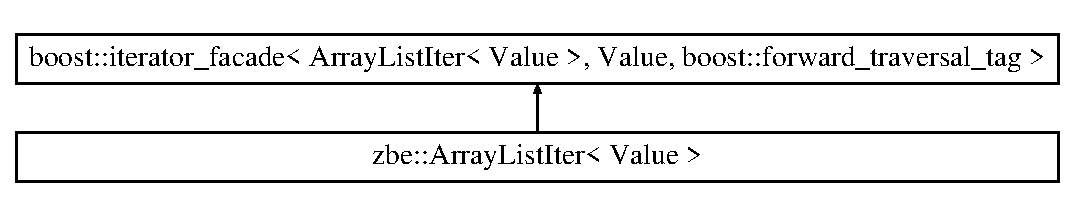
\includegraphics[height=2.000000cm]{classzbe_1_1_array_list_iter}
\end{center}
\end{figure}
\subsection*{Public Member Functions}
\begin{DoxyCompactItemize}
\item 
\hyperlink{classzbe_1_1_array_list_iter_abdbe80b1bb17e316bf91b78a9c161e13}{Array\+List\+Iter} ()
\item 
\hyperlink{classzbe_1_1_array_list_iter_a90f45ad8b761ac282d68e84c830cbad7}{Array\+List\+Iter} (\hyperlink{classzbe_1_1_array_list}{Array\+List}$<$ Value $>$ $\ast$list)
\item 
\hyperlink{classzbe_1_1_array_list_iter_a3ae4ca7a480b4fde8caabe7682a31a24}{Array\+List\+Iter} (\hyperlink{classzbe_1_1_array_list}{Array\+List}$<$ Value $>$ $\ast$list, unsigned i)
\item 
\hyperlink{classzbe_1_1_array_list_iter_a43dd8b2689fa6e354b8fe49475ad45b0}{Array\+List\+Iter} (const \hyperlink{classzbe_1_1_array_list_iter}{Array\+List\+Iter}$<$ Value $>$ \&iter)
\item 
virtual \hyperlink{classzbe_1_1_array_list_iter_aa7e7c9eb567be6062e050919c4da0752}{$\sim$\+Array\+List\+Iter} ()
\end{DoxyCompactItemize}
\subsection*{Friends}
\begin{DoxyCompactItemize}
\item 
class \hyperlink{classzbe_1_1_array_list_iter_ac09f73e325921cc50ebcd96bed0f8096}{boost\+::iterator\+\_\+core\+\_\+access}
\end{DoxyCompactItemize}


\subsection{Detailed Description}
\subsubsection*{template$<$class Value$>$class zbe\+::\+Array\+List\+Iter$<$ Value $>$}



Definition at line 21 of file Array\+List.\+h.



\subsection{Constructor \& Destructor Documentation}
\hypertarget{classzbe_1_1_array_list_iter_abdbe80b1bb17e316bf91b78a9c161e13}{}\index{zbe\+::\+Array\+List\+Iter@{zbe\+::\+Array\+List\+Iter}!Array\+List\+Iter@{Array\+List\+Iter}}
\index{Array\+List\+Iter@{Array\+List\+Iter}!zbe\+::\+Array\+List\+Iter@{zbe\+::\+Array\+List\+Iter}}
\subsubsection[{Array\+List\+Iter()}]{\setlength{\rightskip}{0pt plus 5cm}template$<$class Value$>$ {\bf zbe\+::\+Array\+List\+Iter}$<$ Value $>$\+::{\bf Array\+List\+Iter} (
\begin{DoxyParamCaption}
{}
\end{DoxyParamCaption}
)\hspace{0.3cm}{\ttfamily [inline]}}\label{classzbe_1_1_array_list_iter_abdbe80b1bb17e316bf91b78a9c161e13}


Definition at line 38 of file Array\+List\+Iterator.\+h.

\hypertarget{classzbe_1_1_array_list_iter_a90f45ad8b761ac282d68e84c830cbad7}{}\index{zbe\+::\+Array\+List\+Iter@{zbe\+::\+Array\+List\+Iter}!Array\+List\+Iter@{Array\+List\+Iter}}
\index{Array\+List\+Iter@{Array\+List\+Iter}!zbe\+::\+Array\+List\+Iter@{zbe\+::\+Array\+List\+Iter}}
\subsubsection[{Array\+List\+Iter(\+Array\+List$<$ Value $>$ $\ast$list)}]{\setlength{\rightskip}{0pt plus 5cm}template$<$class Value$>$ {\bf zbe\+::\+Array\+List\+Iter}$<$ Value $>$\+::{\bf Array\+List\+Iter} (
\begin{DoxyParamCaption}
\item[{{\bf Array\+List}$<$ Value $>$ $\ast$}]{list}
\end{DoxyParamCaption}
)\hspace{0.3cm}{\ttfamily [inline]}}\label{classzbe_1_1_array_list_iter_a90f45ad8b761ac282d68e84c830cbad7}


Definition at line 39 of file Array\+List\+Iterator.\+h.

\hypertarget{classzbe_1_1_array_list_iter_a3ae4ca7a480b4fde8caabe7682a31a24}{}\index{zbe\+::\+Array\+List\+Iter@{zbe\+::\+Array\+List\+Iter}!Array\+List\+Iter@{Array\+List\+Iter}}
\index{Array\+List\+Iter@{Array\+List\+Iter}!zbe\+::\+Array\+List\+Iter@{zbe\+::\+Array\+List\+Iter}}
\subsubsection[{Array\+List\+Iter(\+Array\+List$<$ Value $>$ $\ast$list, unsigned i)}]{\setlength{\rightskip}{0pt plus 5cm}template$<$class Value$>$ {\bf zbe\+::\+Array\+List\+Iter}$<$ Value $>$\+::{\bf Array\+List\+Iter} (
\begin{DoxyParamCaption}
\item[{{\bf Array\+List}$<$ Value $>$ $\ast$}]{list, }
\item[{unsigned}]{i}
\end{DoxyParamCaption}
)\hspace{0.3cm}{\ttfamily [inline]}}\label{classzbe_1_1_array_list_iter_a3ae4ca7a480b4fde8caabe7682a31a24}


Definition at line 40 of file Array\+List\+Iterator.\+h.

\hypertarget{classzbe_1_1_array_list_iter_a43dd8b2689fa6e354b8fe49475ad45b0}{}\index{zbe\+::\+Array\+List\+Iter@{zbe\+::\+Array\+List\+Iter}!Array\+List\+Iter@{Array\+List\+Iter}}
\index{Array\+List\+Iter@{Array\+List\+Iter}!zbe\+::\+Array\+List\+Iter@{zbe\+::\+Array\+List\+Iter}}
\subsubsection[{Array\+List\+Iter(const Array\+List\+Iter$<$ Value $>$ \&iter)}]{\setlength{\rightskip}{0pt plus 5cm}template$<$class Value$>$ {\bf zbe\+::\+Array\+List\+Iter}$<$ Value $>$\+::{\bf Array\+List\+Iter} (
\begin{DoxyParamCaption}
\item[{const {\bf Array\+List\+Iter}$<$ Value $>$ \&}]{iter}
\end{DoxyParamCaption}
)\hspace{0.3cm}{\ttfamily [inline]}}\label{classzbe_1_1_array_list_iter_a43dd8b2689fa6e354b8fe49475ad45b0}


Definition at line 41 of file Array\+List\+Iterator.\+h.

\hypertarget{classzbe_1_1_array_list_iter_aa7e7c9eb567be6062e050919c4da0752}{}\index{zbe\+::\+Array\+List\+Iter@{zbe\+::\+Array\+List\+Iter}!````~Array\+List\+Iter@{$\sim$\+Array\+List\+Iter}}
\index{````~Array\+List\+Iter@{$\sim$\+Array\+List\+Iter}!zbe\+::\+Array\+List\+Iter@{zbe\+::\+Array\+List\+Iter}}
\subsubsection[{$\sim$\+Array\+List\+Iter()}]{\setlength{\rightskip}{0pt plus 5cm}template$<$class Value$>$ virtual {\bf zbe\+::\+Array\+List\+Iter}$<$ Value $>$\+::$\sim${\bf Array\+List\+Iter} (
\begin{DoxyParamCaption}
{}
\end{DoxyParamCaption}
)\hspace{0.3cm}{\ttfamily [inline]}, {\ttfamily [virtual]}}\label{classzbe_1_1_array_list_iter_aa7e7c9eb567be6062e050919c4da0752}


Definition at line 43 of file Array\+List\+Iterator.\+h.



\subsection{Friends And Related Function Documentation}
\hypertarget{classzbe_1_1_array_list_iter_ac09f73e325921cc50ebcd96bed0f8096}{}\index{zbe\+::\+Array\+List\+Iter@{zbe\+::\+Array\+List\+Iter}!boost\+::iterator\+\_\+core\+\_\+access@{boost\+::iterator\+\_\+core\+\_\+access}}
\index{boost\+::iterator\+\_\+core\+\_\+access@{boost\+::iterator\+\_\+core\+\_\+access}!zbe\+::\+Array\+List\+Iter@{zbe\+::\+Array\+List\+Iter}}
\subsubsection[{boost\+::iterator\+\_\+core\+\_\+access}]{\setlength{\rightskip}{0pt plus 5cm}template$<$class Value$>$ friend class boost\+::iterator\+\_\+core\+\_\+access\hspace{0.3cm}{\ttfamily [friend]}}\label{classzbe_1_1_array_list_iter_ac09f73e325921cc50ebcd96bed0f8096}


Definition at line 46 of file Array\+List\+Iterator.\+h.



The documentation for this class was generated from the following files\+:\begin{DoxyCompactItemize}
\item 
include/\+Z\+B\+E/core/tools/containers/\hyperlink{_array_list_8h}{Array\+List.\+h}\item 
include/\+Z\+B\+E/core/tools/containers/\hyperlink{_array_list_iterator_8h}{Array\+List\+Iterator.\+h}\end{DoxyCompactItemize}

\hypertarget{structzbe_1_1_array_list_node}{}\section{zbe\+:\+:Array\+List\+Node$<$ Value $>$ Struct Template Reference}
\label{structzbe_1_1_array_list_node}\index{zbe\+::\+Array\+List\+Node$<$ Value $>$@{zbe\+::\+Array\+List\+Node$<$ Value $>$}}


{\ttfamily \#include $<$Array\+List.\+h$>$}

\subsection*{Public Attributes}
\begin{DoxyCompactItemize}
\item 
Value \hyperlink{structzbe_1_1_array_list_node_a4b6ed91c41d1a05f5cbc5a159f27b97d}{value}
\item 
unsigned \hyperlink{structzbe_1_1_array_list_node_a3972b617e2a407a2a601a027b516980e}{next}
\end{DoxyCompactItemize}


\subsection{Detailed Description}
\subsubsection*{template$<$class Value$>$struct zbe\+::\+Array\+List\+Node$<$ Value $>$}



Definition at line 24 of file Array\+List.\+h.



\subsection{Member Data Documentation}
\hypertarget{structzbe_1_1_array_list_node_a3972b617e2a407a2a601a027b516980e}{}\index{zbe\+::\+Array\+List\+Node@{zbe\+::\+Array\+List\+Node}!next@{next}}
\index{next@{next}!zbe\+::\+Array\+List\+Node@{zbe\+::\+Array\+List\+Node}}
\subsubsection[{next}]{\setlength{\rightskip}{0pt plus 5cm}template$<$class Value$>$ unsigned {\bf zbe\+::\+Array\+List\+Node}$<$ Value $>$\+::next}\label{structzbe_1_1_array_list_node_a3972b617e2a407a2a601a027b516980e}


Definition at line 26 of file Array\+List.\+h.

\hypertarget{structzbe_1_1_array_list_node_a4b6ed91c41d1a05f5cbc5a159f27b97d}{}\index{zbe\+::\+Array\+List\+Node@{zbe\+::\+Array\+List\+Node}!value@{value}}
\index{value@{value}!zbe\+::\+Array\+List\+Node@{zbe\+::\+Array\+List\+Node}}
\subsubsection[{value}]{\setlength{\rightskip}{0pt plus 5cm}template$<$class Value$>$ Value {\bf zbe\+::\+Array\+List\+Node}$<$ Value $>$\+::value}\label{structzbe_1_1_array_list_node_a4b6ed91c41d1a05f5cbc5a159f27b97d}


Definition at line 25 of file Array\+List.\+h.



The documentation for this struct was generated from the following file\+:\begin{DoxyCompactItemize}
\item 
include/\+Z\+B\+E/core/tools/containers/\hyperlink{_array_list_8h}{Array\+List.\+h}\end{DoxyCompactItemize}

\hypertarget{classzbe_1_1_array_list_ticketed}{}\section{zbe\+:\+:Array\+List\+Ticketed$<$ Value $>$ Class Template Reference}
\label{classzbe_1_1_array_list_ticketed}\index{zbe\+::\+Array\+List\+Ticketed$<$ Value $>$@{zbe\+::\+Array\+List\+Ticketed$<$ Value $>$}}


{\ttfamily \#include $<$Array\+List.\+h$>$}

\subsection*{Public Member Functions}
\begin{DoxyCompactItemize}
\item 
\hyperlink{classzbe_1_1_array_list_ticketed_afff5d9befd97a0d129ba81a5c2f182fa}{Array\+List\+Ticketed} (unsigned capacity)
\item 
virtual \hyperlink{classzbe_1_1_array_list_ticketed_a1224fa84d15f3ecb76b2a445fd00a397}{$\sim$\+Array\+List\+Ticketed} ()
\item 
\hyperlink{classzbe_1_1_ticket}{Ticket} \& \hyperlink{classzbe_1_1_array_list_ticketed_a163e622f9ff8e9212237edd5069b0cf7}{insert} (Value value)
\item 
unsigned \hyperlink{classzbe_1_1_array_list_ticketed_ae364fce45b2e1ac2c0d88cdba6550bc3}{get\+Capacity} ()
\item 
unsigned \hyperlink{classzbe_1_1_array_list_ticketed_adfaa36ca3a1324289f3c62b89b8cbebb}{get\+Size} ()
\item 
bool \hyperlink{classzbe_1_1_array_list_ticketed_aa602a202649a4fd159b64a6598aa2187}{is\+Empty} ()
\item 
\hyperlink{classzbe_1_1_array_list_ticketed_iter}{Array\+List\+Ticketed\+Iter}$<$ Value $>$ \hyperlink{classzbe_1_1_array_list_ticketed_a580db1c605df628c8c87c936d6c18e43}{begin} ()
\item 
\hyperlink{classzbe_1_1_array_list_ticketed_iter}{Array\+List\+Ticketed\+Iter}$<$ Value $>$ \hyperlink{classzbe_1_1_array_list_ticketed_a5033c9e9335b4518604be7e3bb5a95ac}{end} ()
\item 
\hyperlink{structzbe_1_1_array_list_ticketed_node}{Array\+List\+Ticketed\+Node}$<$ Value $>$ \& \hyperlink{classzbe_1_1_array_list_ticketed_a6a4bb7e7e487d8bf85523aacfca64291}{operator\mbox{[}$\,$\mbox{]}} (unsigned idx)
\item 
const \hyperlink{structzbe_1_1_array_list_ticketed_node}{Array\+List\+Ticketed\+Node}$<$ Value $>$ \& \hyperlink{classzbe_1_1_array_list_ticketed_ad61ad37401c3727a026432e00c90b480}{operator\mbox{[}$\,$\mbox{]}} (unsigned idx) const 
\end{DoxyCompactItemize}
\subsection*{Friends}
\begin{DoxyCompactItemize}
\item 
class \hyperlink{classzbe_1_1_array_list_ticketed_a57b86bbf01926226da6fa92bc31b0c5d}{Array\+List\+Ticketed\+Iter$<$ Value $>$}
\end{DoxyCompactItemize}


\subsection{Detailed Description}
\subsubsection*{template$<$class Value$>$class zbe\+::\+Array\+List\+Ticketed$<$ Value $>$}



Definition at line 126 of file Array\+List.\+h.



\subsection{Constructor \& Destructor Documentation}
\hypertarget{classzbe_1_1_array_list_ticketed_afff5d9befd97a0d129ba81a5c2f182fa}{}\index{zbe\+::\+Array\+List\+Ticketed@{zbe\+::\+Array\+List\+Ticketed}!Array\+List\+Ticketed@{Array\+List\+Ticketed}}
\index{Array\+List\+Ticketed@{Array\+List\+Ticketed}!zbe\+::\+Array\+List\+Ticketed@{zbe\+::\+Array\+List\+Ticketed}}
\subsubsection[{Array\+List\+Ticketed(unsigned capacity)}]{\setlength{\rightskip}{0pt plus 5cm}template$<$class Value $>$ {\bf zbe\+::\+Array\+List\+Ticketed}$<$ Value $>$\+::{\bf Array\+List\+Ticketed} (
\begin{DoxyParamCaption}
\item[{unsigned}]{capacity}
\end{DoxyParamCaption}
)}\label{classzbe_1_1_array_list_ticketed_afff5d9befd97a0d129ba81a5c2f182fa}


Definition at line 158 of file Array\+List.\+h.

\hypertarget{classzbe_1_1_array_list_ticketed_a1224fa84d15f3ecb76b2a445fd00a397}{}\index{zbe\+::\+Array\+List\+Ticketed@{zbe\+::\+Array\+List\+Ticketed}!````~Array\+List\+Ticketed@{$\sim$\+Array\+List\+Ticketed}}
\index{````~Array\+List\+Ticketed@{$\sim$\+Array\+List\+Ticketed}!zbe\+::\+Array\+List\+Ticketed@{zbe\+::\+Array\+List\+Ticketed}}
\subsubsection[{$\sim$\+Array\+List\+Ticketed()}]{\setlength{\rightskip}{0pt plus 5cm}template$<$class Value $>$ {\bf zbe\+::\+Array\+List\+Ticketed}$<$ Value $>$\+::$\sim${\bf Array\+List\+Ticketed} (
\begin{DoxyParamCaption}
{}
\end{DoxyParamCaption}
)\hspace{0.3cm}{\ttfamily [virtual]}}\label{classzbe_1_1_array_list_ticketed_a1224fa84d15f3ecb76b2a445fd00a397}


Definition at line 181 of file Array\+List.\+h.



\subsection{Member Function Documentation}
\hypertarget{classzbe_1_1_array_list_ticketed_a580db1c605df628c8c87c936d6c18e43}{}\index{zbe\+::\+Array\+List\+Ticketed@{zbe\+::\+Array\+List\+Ticketed}!begin@{begin}}
\index{begin@{begin}!zbe\+::\+Array\+List\+Ticketed@{zbe\+::\+Array\+List\+Ticketed}}
\subsubsection[{begin()}]{\setlength{\rightskip}{0pt plus 5cm}template$<$class Value$>$ {\bf Array\+List\+Ticketed\+Iter}$<$Value$>$ {\bf zbe\+::\+Array\+List\+Ticketed}$<$ Value $>$\+::begin (
\begin{DoxyParamCaption}
{}
\end{DoxyParamCaption}
)\hspace{0.3cm}{\ttfamily [inline]}}\label{classzbe_1_1_array_list_ticketed_a580db1c605df628c8c87c936d6c18e43}


Definition at line 141 of file Array\+List.\+h.

\hypertarget{classzbe_1_1_array_list_ticketed_a5033c9e9335b4518604be7e3bb5a95ac}{}\index{zbe\+::\+Array\+List\+Ticketed@{zbe\+::\+Array\+List\+Ticketed}!end@{end}}
\index{end@{end}!zbe\+::\+Array\+List\+Ticketed@{zbe\+::\+Array\+List\+Ticketed}}
\subsubsection[{end()}]{\setlength{\rightskip}{0pt plus 5cm}template$<$class Value$>$ {\bf Array\+List\+Ticketed\+Iter}$<$Value$>$ {\bf zbe\+::\+Array\+List\+Ticketed}$<$ Value $>$\+::end (
\begin{DoxyParamCaption}
{}
\end{DoxyParamCaption}
)\hspace{0.3cm}{\ttfamily [inline]}}\label{classzbe_1_1_array_list_ticketed_a5033c9e9335b4518604be7e3bb5a95ac}


Definition at line 142 of file Array\+List.\+h.

\hypertarget{classzbe_1_1_array_list_ticketed_ae364fce45b2e1ac2c0d88cdba6550bc3}{}\index{zbe\+::\+Array\+List\+Ticketed@{zbe\+::\+Array\+List\+Ticketed}!get\+Capacity@{get\+Capacity}}
\index{get\+Capacity@{get\+Capacity}!zbe\+::\+Array\+List\+Ticketed@{zbe\+::\+Array\+List\+Ticketed}}
\subsubsection[{get\+Capacity()}]{\setlength{\rightskip}{0pt plus 5cm}template$<$class Value$>$ unsigned {\bf zbe\+::\+Array\+List\+Ticketed}$<$ Value $>$\+::get\+Capacity (
\begin{DoxyParamCaption}
{}
\end{DoxyParamCaption}
)\hspace{0.3cm}{\ttfamily [inline]}}\label{classzbe_1_1_array_list_ticketed_ae364fce45b2e1ac2c0d88cdba6550bc3}


Definition at line 136 of file Array\+List.\+h.

\hypertarget{classzbe_1_1_array_list_ticketed_adfaa36ca3a1324289f3c62b89b8cbebb}{}\index{zbe\+::\+Array\+List\+Ticketed@{zbe\+::\+Array\+List\+Ticketed}!get\+Size@{get\+Size}}
\index{get\+Size@{get\+Size}!zbe\+::\+Array\+List\+Ticketed@{zbe\+::\+Array\+List\+Ticketed}}
\subsubsection[{get\+Size()}]{\setlength{\rightskip}{0pt plus 5cm}template$<$class Value$>$ unsigned {\bf zbe\+::\+Array\+List\+Ticketed}$<$ Value $>$\+::get\+Size (
\begin{DoxyParamCaption}
{}
\end{DoxyParamCaption}
)\hspace{0.3cm}{\ttfamily [inline]}}\label{classzbe_1_1_array_list_ticketed_adfaa36ca3a1324289f3c62b89b8cbebb}


Definition at line 137 of file Array\+List.\+h.

\hypertarget{classzbe_1_1_array_list_ticketed_a163e622f9ff8e9212237edd5069b0cf7}{}\index{zbe\+::\+Array\+List\+Ticketed@{zbe\+::\+Array\+List\+Ticketed}!insert@{insert}}
\index{insert@{insert}!zbe\+::\+Array\+List\+Ticketed@{zbe\+::\+Array\+List\+Ticketed}}
\subsubsection[{insert(\+Value value)}]{\setlength{\rightskip}{0pt plus 5cm}template$<$class Value $>$ {\bf Ticket} \& {\bf zbe\+::\+Array\+List\+Ticketed}$<$ Value $>$\+::insert (
\begin{DoxyParamCaption}
\item[{Value}]{value}
\end{DoxyParamCaption}
)}\label{classzbe_1_1_array_list_ticketed_a163e622f9ff8e9212237edd5069b0cf7}


Definition at line 186 of file Array\+List.\+h.

\hypertarget{classzbe_1_1_array_list_ticketed_aa602a202649a4fd159b64a6598aa2187}{}\index{zbe\+::\+Array\+List\+Ticketed@{zbe\+::\+Array\+List\+Ticketed}!is\+Empty@{is\+Empty}}
\index{is\+Empty@{is\+Empty}!zbe\+::\+Array\+List\+Ticketed@{zbe\+::\+Array\+List\+Ticketed}}
\subsubsection[{is\+Empty()}]{\setlength{\rightskip}{0pt plus 5cm}template$<$class Value$>$ bool {\bf zbe\+::\+Array\+List\+Ticketed}$<$ Value $>$\+::is\+Empty (
\begin{DoxyParamCaption}
{}
\end{DoxyParamCaption}
)\hspace{0.3cm}{\ttfamily [inline]}}\label{classzbe_1_1_array_list_ticketed_aa602a202649a4fd159b64a6598aa2187}


Definition at line 139 of file Array\+List.\+h.

\hypertarget{classzbe_1_1_array_list_ticketed_a6a4bb7e7e487d8bf85523aacfca64291}{}\index{zbe\+::\+Array\+List\+Ticketed@{zbe\+::\+Array\+List\+Ticketed}!operator\mbox{[}$\,$\mbox{]}@{operator[]}}
\index{operator\mbox{[}$\,$\mbox{]}@{operator[]}!zbe\+::\+Array\+List\+Ticketed@{zbe\+::\+Array\+List\+Ticketed}}
\subsubsection[{operator[](unsigned idx)}]{\setlength{\rightskip}{0pt plus 5cm}template$<$class Value $>$ {\bf Array\+List\+Ticketed\+Node}$<$ Value $>$ \& {\bf zbe\+::\+Array\+List\+Ticketed}$<$ Value $>$\+::operator\mbox{[}$\,$\mbox{]} (
\begin{DoxyParamCaption}
\item[{unsigned}]{idx}
\end{DoxyParamCaption}
)}\label{classzbe_1_1_array_list_ticketed_a6a4bb7e7e487d8bf85523aacfca64291}


Definition at line 202 of file Array\+List.\+h.

\hypertarget{classzbe_1_1_array_list_ticketed_ad61ad37401c3727a026432e00c90b480}{}\index{zbe\+::\+Array\+List\+Ticketed@{zbe\+::\+Array\+List\+Ticketed}!operator\mbox{[}$\,$\mbox{]}@{operator[]}}
\index{operator\mbox{[}$\,$\mbox{]}@{operator[]}!zbe\+::\+Array\+List\+Ticketed@{zbe\+::\+Array\+List\+Ticketed}}
\subsubsection[{operator[](unsigned idx) const }]{\setlength{\rightskip}{0pt plus 5cm}template$<$class Value $>$ const {\bf Array\+List\+Ticketed\+Node}$<$ Value $>$ \& {\bf zbe\+::\+Array\+List\+Ticketed}$<$ Value $>$\+::operator\mbox{[}$\,$\mbox{]} (
\begin{DoxyParamCaption}
\item[{unsigned}]{idx}
\end{DoxyParamCaption}
) const}\label{classzbe_1_1_array_list_ticketed_ad61ad37401c3727a026432e00c90b480}


Definition at line 207 of file Array\+List.\+h.



\subsection{Friends And Related Function Documentation}
\hypertarget{classzbe_1_1_array_list_ticketed_a57b86bbf01926226da6fa92bc31b0c5d}{}\index{zbe\+::\+Array\+List\+Ticketed@{zbe\+::\+Array\+List\+Ticketed}!Array\+List\+Ticketed\+Iter$<$ Value $>$@{Array\+List\+Ticketed\+Iter$<$ Value $>$}}
\index{Array\+List\+Ticketed\+Iter$<$ Value $>$@{Array\+List\+Ticketed\+Iter$<$ Value $>$}!zbe\+::\+Array\+List\+Ticketed@{zbe\+::\+Array\+List\+Ticketed}}
\subsubsection[{Array\+List\+Ticketed\+Iter$<$ Value $>$}]{\setlength{\rightskip}{0pt plus 5cm}template$<$class Value$>$ friend class {\bf Array\+List\+Ticketed\+Iter}$<$ Value $>$\hspace{0.3cm}{\ttfamily [friend]}}\label{classzbe_1_1_array_list_ticketed_a57b86bbf01926226da6fa92bc31b0c5d}


Definition at line 148 of file Array\+List.\+h.



The documentation for this class was generated from the following file\+:\begin{DoxyCompactItemize}
\item 
include/\+Z\+B\+E/core/tools/containers/\hyperlink{_array_list_8h}{Array\+List.\+h}\end{DoxyCompactItemize}

\hypertarget{classzbe_1_1_array_list_ticketed_iter}{}\section{zbe\+:\+:Array\+List\+Ticketed\+Iter$<$ Value $>$ Class Template Reference}
\label{classzbe_1_1_array_list_ticketed_iter}\index{zbe\+::\+Array\+List\+Ticketed\+Iter$<$ Value $>$@{zbe\+::\+Array\+List\+Ticketed\+Iter$<$ Value $>$}}


{\ttfamily \#include $<$Array\+List.\+h$>$}

Inheritance diagram for zbe\+:\+:Array\+List\+Ticketed\+Iter$<$ Value $>$\+:\begin{figure}[H]
\begin{center}
\leavevmode
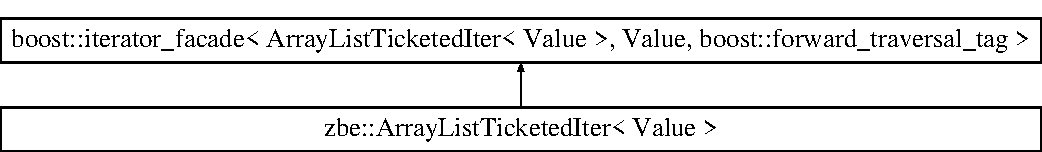
\includegraphics[height=2.000000cm]{classzbe_1_1_array_list_ticketed_iter}
\end{center}
\end{figure}
\subsection*{Public Member Functions}
\begin{DoxyCompactItemize}
\item 
\hyperlink{classzbe_1_1_array_list_ticketed_iter_a66a8dcea6526d7d4182de6ffc75b512f}{Array\+List\+Ticketed\+Iter} ()
\item 
\hyperlink{classzbe_1_1_array_list_ticketed_iter_a682af187999fffe8df2c05b60c089820}{Array\+List\+Ticketed\+Iter} (\hyperlink{classzbe_1_1_array_list_ticketed}{Array\+List\+Ticketed}$<$ Value $>$ $\ast$list)
\item 
\hyperlink{classzbe_1_1_array_list_ticketed_iter_a1446852d8925958aa59fb6bb61913583}{Array\+List\+Ticketed\+Iter} (\hyperlink{classzbe_1_1_array_list_ticketed}{Array\+List\+Ticketed}$<$ Value $>$ $\ast$list, unsigned i)
\item 
\hyperlink{classzbe_1_1_array_list_ticketed_iter_a11ce77f4b4fd98ce4b02e9b6bbba50a9}{Array\+List\+Ticketed\+Iter} (const \hyperlink{classzbe_1_1_array_list_ticketed_iter}{Array\+List\+Ticketed\+Iter}$<$ Value $>$ \&iter)
\item 
virtual \hyperlink{classzbe_1_1_array_list_ticketed_iter_a59be66018a5a0f330d1708c2d36f63c9}{$\sim$\+Array\+List\+Ticketed\+Iter} ()
\item 
void \hyperlink{classzbe_1_1_array_list_ticketed_iter_a2780208a2abb45fceb786bf93489a4dc}{reset} ()
\end{DoxyCompactItemize}
\subsection*{Friends}
\begin{DoxyCompactItemize}
\item 
class \hyperlink{classzbe_1_1_array_list_ticketed_iter_ac09f73e325921cc50ebcd96bed0f8096}{boost\+::iterator\+\_\+core\+\_\+access}
\end{DoxyCompactItemize}


\subsection{Detailed Description}
\subsubsection*{template$<$class Value$>$class zbe\+::\+Array\+List\+Ticketed\+Iter$<$ Value $>$}



Definition at line 116 of file Array\+List.\+h.



\subsection{Constructor \& Destructor Documentation}
\hypertarget{classzbe_1_1_array_list_ticketed_iter_a66a8dcea6526d7d4182de6ffc75b512f}{}\index{zbe\+::\+Array\+List\+Ticketed\+Iter@{zbe\+::\+Array\+List\+Ticketed\+Iter}!Array\+List\+Ticketed\+Iter@{Array\+List\+Ticketed\+Iter}}
\index{Array\+List\+Ticketed\+Iter@{Array\+List\+Ticketed\+Iter}!zbe\+::\+Array\+List\+Ticketed\+Iter@{zbe\+::\+Array\+List\+Ticketed\+Iter}}
\subsubsection[{Array\+List\+Ticketed\+Iter()}]{\setlength{\rightskip}{0pt plus 5cm}template$<$class Value$>$ {\bf zbe\+::\+Array\+List\+Ticketed\+Iter}$<$ Value $>$\+::{\bf Array\+List\+Ticketed\+Iter} (
\begin{DoxyParamCaption}
{}
\end{DoxyParamCaption}
)\hspace{0.3cm}{\ttfamily [inline]}}\label{classzbe_1_1_array_list_ticketed_iter_a66a8dcea6526d7d4182de6ffc75b512f}


Definition at line 87 of file Array\+List\+Iterator.\+h.

\hypertarget{classzbe_1_1_array_list_ticketed_iter_a682af187999fffe8df2c05b60c089820}{}\index{zbe\+::\+Array\+List\+Ticketed\+Iter@{zbe\+::\+Array\+List\+Ticketed\+Iter}!Array\+List\+Ticketed\+Iter@{Array\+List\+Ticketed\+Iter}}
\index{Array\+List\+Ticketed\+Iter@{Array\+List\+Ticketed\+Iter}!zbe\+::\+Array\+List\+Ticketed\+Iter@{zbe\+::\+Array\+List\+Ticketed\+Iter}}
\subsubsection[{Array\+List\+Ticketed\+Iter(\+Array\+List\+Ticketed$<$ Value $>$ $\ast$list)}]{\setlength{\rightskip}{0pt plus 5cm}template$<$class Value$>$ {\bf zbe\+::\+Array\+List\+Ticketed\+Iter}$<$ Value $>$\+::{\bf Array\+List\+Ticketed\+Iter} (
\begin{DoxyParamCaption}
\item[{{\bf Array\+List\+Ticketed}$<$ Value $>$ $\ast$}]{list}
\end{DoxyParamCaption}
)\hspace{0.3cm}{\ttfamily [inline]}}\label{classzbe_1_1_array_list_ticketed_iter_a682af187999fffe8df2c05b60c089820}


Definition at line 88 of file Array\+List\+Iterator.\+h.

\hypertarget{classzbe_1_1_array_list_ticketed_iter_a1446852d8925958aa59fb6bb61913583}{}\index{zbe\+::\+Array\+List\+Ticketed\+Iter@{zbe\+::\+Array\+List\+Ticketed\+Iter}!Array\+List\+Ticketed\+Iter@{Array\+List\+Ticketed\+Iter}}
\index{Array\+List\+Ticketed\+Iter@{Array\+List\+Ticketed\+Iter}!zbe\+::\+Array\+List\+Ticketed\+Iter@{zbe\+::\+Array\+List\+Ticketed\+Iter}}
\subsubsection[{Array\+List\+Ticketed\+Iter(\+Array\+List\+Ticketed$<$ Value $>$ $\ast$list, unsigned i)}]{\setlength{\rightskip}{0pt plus 5cm}template$<$class Value$>$ {\bf zbe\+::\+Array\+List\+Ticketed\+Iter}$<$ Value $>$\+::{\bf Array\+List\+Ticketed\+Iter} (
\begin{DoxyParamCaption}
\item[{{\bf Array\+List\+Ticketed}$<$ Value $>$ $\ast$}]{list, }
\item[{unsigned}]{i}
\end{DoxyParamCaption}
)\hspace{0.3cm}{\ttfamily [inline]}}\label{classzbe_1_1_array_list_ticketed_iter_a1446852d8925958aa59fb6bb61913583}


Definition at line 89 of file Array\+List\+Iterator.\+h.

\hypertarget{classzbe_1_1_array_list_ticketed_iter_a11ce77f4b4fd98ce4b02e9b6bbba50a9}{}\index{zbe\+::\+Array\+List\+Ticketed\+Iter@{zbe\+::\+Array\+List\+Ticketed\+Iter}!Array\+List\+Ticketed\+Iter@{Array\+List\+Ticketed\+Iter}}
\index{Array\+List\+Ticketed\+Iter@{Array\+List\+Ticketed\+Iter}!zbe\+::\+Array\+List\+Ticketed\+Iter@{zbe\+::\+Array\+List\+Ticketed\+Iter}}
\subsubsection[{Array\+List\+Ticketed\+Iter(const Array\+List\+Ticketed\+Iter$<$ Value $>$ \&iter)}]{\setlength{\rightskip}{0pt plus 5cm}template$<$class Value$>$ {\bf zbe\+::\+Array\+List\+Ticketed\+Iter}$<$ Value $>$\+::{\bf Array\+List\+Ticketed\+Iter} (
\begin{DoxyParamCaption}
\item[{const {\bf Array\+List\+Ticketed\+Iter}$<$ Value $>$ \&}]{iter}
\end{DoxyParamCaption}
)\hspace{0.3cm}{\ttfamily [inline]}}\label{classzbe_1_1_array_list_ticketed_iter_a11ce77f4b4fd98ce4b02e9b6bbba50a9}


Definition at line 90 of file Array\+List\+Iterator.\+h.

\hypertarget{classzbe_1_1_array_list_ticketed_iter_a59be66018a5a0f330d1708c2d36f63c9}{}\index{zbe\+::\+Array\+List\+Ticketed\+Iter@{zbe\+::\+Array\+List\+Ticketed\+Iter}!````~Array\+List\+Ticketed\+Iter@{$\sim$\+Array\+List\+Ticketed\+Iter}}
\index{````~Array\+List\+Ticketed\+Iter@{$\sim$\+Array\+List\+Ticketed\+Iter}!zbe\+::\+Array\+List\+Ticketed\+Iter@{zbe\+::\+Array\+List\+Ticketed\+Iter}}
\subsubsection[{$\sim$\+Array\+List\+Ticketed\+Iter()}]{\setlength{\rightskip}{0pt plus 5cm}template$<$class Value$>$ virtual {\bf zbe\+::\+Array\+List\+Ticketed\+Iter}$<$ Value $>$\+::$\sim${\bf Array\+List\+Ticketed\+Iter} (
\begin{DoxyParamCaption}
{}
\end{DoxyParamCaption}
)\hspace{0.3cm}{\ttfamily [inline]}, {\ttfamily [virtual]}}\label{classzbe_1_1_array_list_ticketed_iter_a59be66018a5a0f330d1708c2d36f63c9}


Definition at line 92 of file Array\+List\+Iterator.\+h.



\subsection{Member Function Documentation}
\hypertarget{classzbe_1_1_array_list_ticketed_iter_a2780208a2abb45fceb786bf93489a4dc}{}\index{zbe\+::\+Array\+List\+Ticketed\+Iter@{zbe\+::\+Array\+List\+Ticketed\+Iter}!reset@{reset}}
\index{reset@{reset}!zbe\+::\+Array\+List\+Ticketed\+Iter@{zbe\+::\+Array\+List\+Ticketed\+Iter}}
\subsubsection[{reset()}]{\setlength{\rightskip}{0pt plus 5cm}template$<$class Value$>$ void {\bf zbe\+::\+Array\+List\+Ticketed\+Iter}$<$ Value $>$\+::reset (
\begin{DoxyParamCaption}
{}
\end{DoxyParamCaption}
)\hspace{0.3cm}{\ttfamily [inline]}}\label{classzbe_1_1_array_list_ticketed_iter_a2780208a2abb45fceb786bf93489a4dc}


Definition at line 96 of file Array\+List\+Iterator.\+h.



\subsection{Friends And Related Function Documentation}
\hypertarget{classzbe_1_1_array_list_ticketed_iter_ac09f73e325921cc50ebcd96bed0f8096}{}\index{zbe\+::\+Array\+List\+Ticketed\+Iter@{zbe\+::\+Array\+List\+Ticketed\+Iter}!boost\+::iterator\+\_\+core\+\_\+access@{boost\+::iterator\+\_\+core\+\_\+access}}
\index{boost\+::iterator\+\_\+core\+\_\+access@{boost\+::iterator\+\_\+core\+\_\+access}!zbe\+::\+Array\+List\+Ticketed\+Iter@{zbe\+::\+Array\+List\+Ticketed\+Iter}}
\subsubsection[{boost\+::iterator\+\_\+core\+\_\+access}]{\setlength{\rightskip}{0pt plus 5cm}template$<$class Value$>$ friend class boost\+::iterator\+\_\+core\+\_\+access\hspace{0.3cm}{\ttfamily [friend]}}\label{classzbe_1_1_array_list_ticketed_iter_ac09f73e325921cc50ebcd96bed0f8096}


Definition at line 106 of file Array\+List\+Iterator.\+h.



The documentation for this class was generated from the following files\+:\begin{DoxyCompactItemize}
\item 
include/\+Z\+B\+E/core/tools/containers/\hyperlink{_array_list_8h}{Array\+List.\+h}\item 
include/\+Z\+B\+E/core/tools/containers/\hyperlink{_array_list_iterator_8h}{Array\+List\+Iterator.\+h}\end{DoxyCompactItemize}

\hypertarget{structzbe_1_1_array_list_ticketed_node}{}\section{zbe\+:\+:Array\+List\+Ticketed\+Node$<$ Value $>$ Struct Template Reference}
\label{structzbe_1_1_array_list_ticketed_node}\index{zbe\+::\+Array\+List\+Ticketed\+Node$<$ Value $>$@{zbe\+::\+Array\+List\+Ticketed\+Node$<$ Value $>$}}


{\ttfamily \#include $<$Array\+List.\+h$>$}

\subsection*{Public Attributes}
\begin{DoxyCompactItemize}
\item 
Value \hyperlink{structzbe_1_1_array_list_ticketed_node_ae04e02e278b795dc6f657df33b0d52e1}{v}
\item 
int \hyperlink{structzbe_1_1_array_list_ticketed_node_a5a8f613daae38000942031888f3f8d52}{next}
\item 
\hyperlink{classzbe_1_1_ticket}{Ticket} \hyperlink{structzbe_1_1_array_list_ticketed_node_a4bef8c634cd8a3a31f20c1720a05a2fc}{t}
\end{DoxyCompactItemize}


\subsection{Detailed Description}
\subsubsection*{template$<$class Value$>$struct zbe\+::\+Array\+List\+Ticketed\+Node$<$ Value $>$}



Definition at line 119 of file Array\+List.\+h.



\subsection{Member Data Documentation}
\hypertarget{structzbe_1_1_array_list_ticketed_node_a5a8f613daae38000942031888f3f8d52}{}\index{zbe\+::\+Array\+List\+Ticketed\+Node@{zbe\+::\+Array\+List\+Ticketed\+Node}!next@{next}}
\index{next@{next}!zbe\+::\+Array\+List\+Ticketed\+Node@{zbe\+::\+Array\+List\+Ticketed\+Node}}
\subsubsection[{next}]{\setlength{\rightskip}{0pt plus 5cm}template$<$class Value$>$ int {\bf zbe\+::\+Array\+List\+Ticketed\+Node}$<$ Value $>$\+::next}\label{structzbe_1_1_array_list_ticketed_node_a5a8f613daae38000942031888f3f8d52}


Definition at line 121 of file Array\+List.\+h.

\hypertarget{structzbe_1_1_array_list_ticketed_node_a4bef8c634cd8a3a31f20c1720a05a2fc}{}\index{zbe\+::\+Array\+List\+Ticketed\+Node@{zbe\+::\+Array\+List\+Ticketed\+Node}!t@{t}}
\index{t@{t}!zbe\+::\+Array\+List\+Ticketed\+Node@{zbe\+::\+Array\+List\+Ticketed\+Node}}
\subsubsection[{t}]{\setlength{\rightskip}{0pt plus 5cm}template$<$class Value$>$ {\bf Ticket} {\bf zbe\+::\+Array\+List\+Ticketed\+Node}$<$ Value $>$\+::t}\label{structzbe_1_1_array_list_ticketed_node_a4bef8c634cd8a3a31f20c1720a05a2fc}


Definition at line 122 of file Array\+List.\+h.

\hypertarget{structzbe_1_1_array_list_ticketed_node_ae04e02e278b795dc6f657df33b0d52e1}{}\index{zbe\+::\+Array\+List\+Ticketed\+Node@{zbe\+::\+Array\+List\+Ticketed\+Node}!v@{v}}
\index{v@{v}!zbe\+::\+Array\+List\+Ticketed\+Node@{zbe\+::\+Array\+List\+Ticketed\+Node}}
\subsubsection[{v}]{\setlength{\rightskip}{0pt plus 5cm}template$<$class Value$>$ Value {\bf zbe\+::\+Array\+List\+Ticketed\+Node}$<$ Value $>$\+::v}\label{structzbe_1_1_array_list_ticketed_node_ae04e02e278b795dc6f657df33b0d52e1}


Definition at line 120 of file Array\+List.\+h.



The documentation for this struct was generated from the following file\+:\begin{DoxyCompactItemize}
\item 
include/\+Z\+B\+E/core/tools/containers/\hyperlink{_array_list_8h}{Array\+List.\+h}\end{DoxyCompactItemize}

\hypertarget{classzbe_1_1_behavior}{}\section{zbe\+:\+:Behavior Class Reference}
\label{classzbe_1_1_behavior}\index{zbe\+::\+Behavior@{zbe\+::\+Behavior}}


{\ttfamily \#include $<$Behavior.\+h$>$}

Inheritance diagram for zbe\+:\+:Behavior\+:\begin{figure}[H]
\begin{center}
\leavevmode
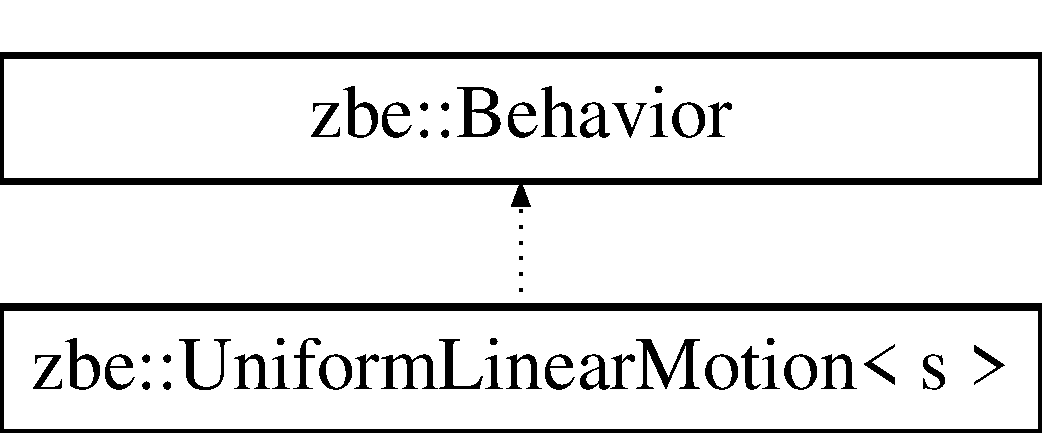
\includegraphics[height=2.000000cm]{classzbe_1_1_behavior}
\end{center}
\end{figure}
\subsection*{Public Member Functions}
\begin{DoxyCompactItemize}
\item 
virtual \hyperlink{classzbe_1_1_behavior_a7c1f04feb979320c55591e765cf817a9}{$\sim$\+Behavior} ()
\item 
virtual void \hyperlink{classzbe_1_1_behavior_a9bd7af2d6f39aafb11052e2ebdca3a71}{behave\+Until} (double time)=0
\end{DoxyCompactItemize}


\subsection{Detailed Description}


Definition at line 15 of file Behavior.\+h.



\subsection{Constructor \& Destructor Documentation}
\hypertarget{classzbe_1_1_behavior_a7c1f04feb979320c55591e765cf817a9}{}\index{zbe\+::\+Behavior@{zbe\+::\+Behavior}!````~Behavior@{$\sim$\+Behavior}}
\index{````~Behavior@{$\sim$\+Behavior}!zbe\+::\+Behavior@{zbe\+::\+Behavior}}
\subsubsection[{$\sim$\+Behavior()}]{\setlength{\rightskip}{0pt plus 5cm}virtual zbe\+::\+Behavior\+::$\sim$\+Behavior (
\begin{DoxyParamCaption}
{}
\end{DoxyParamCaption}
)\hspace{0.3cm}{\ttfamily [inline]}, {\ttfamily [virtual]}}\label{classzbe_1_1_behavior_a7c1f04feb979320c55591e765cf817a9}


Definition at line 17 of file Behavior.\+h.



\subsection{Member Function Documentation}
\hypertarget{classzbe_1_1_behavior_a9bd7af2d6f39aafb11052e2ebdca3a71}{}\index{zbe\+::\+Behavior@{zbe\+::\+Behavior}!behave\+Until@{behave\+Until}}
\index{behave\+Until@{behave\+Until}!zbe\+::\+Behavior@{zbe\+::\+Behavior}}
\subsubsection[{behave\+Until(double time)=0}]{\setlength{\rightskip}{0pt plus 5cm}virtual void zbe\+::\+Behavior\+::behave\+Until (
\begin{DoxyParamCaption}
\item[{double}]{time}
\end{DoxyParamCaption}
)\hspace{0.3cm}{\ttfamily [pure virtual]}}\label{classzbe_1_1_behavior_a9bd7af2d6f39aafb11052e2ebdca3a71}


Implemented in \hyperlink{classzbe_1_1_uniform_linear_motion_a42678dd6e10f13645574f5e41611de82}{zbe\+::\+Uniform\+Linear\+Motion$<$ s $>$}.



The documentation for this class was generated from the following file\+:\begin{DoxyCompactItemize}
\item 
include/\+Z\+B\+E/core/behaviors/\hyperlink{_behavior_8h}{Behavior.\+h}\end{DoxyCompactItemize}

\hypertarget{structzbe_1_1_circle}{}\section{zbe\+:\+:Circle Struct Reference}
\label{structzbe_1_1_circle}\index{zbe\+::\+Circle@{zbe\+::\+Circle}}


{\ttfamily \#include $<$objects.\+h$>$}

Inheritance diagram for zbe\+:\+:Circle\+:\begin{figure}[H]
\begin{center}
\leavevmode
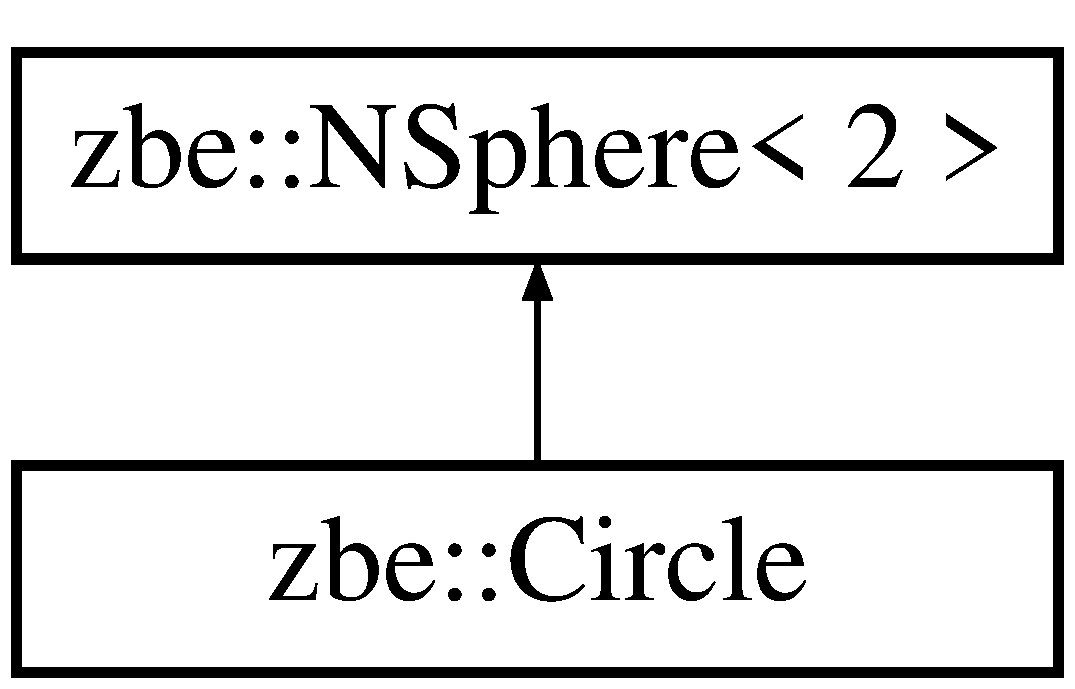
\includegraphics[height=2.000000cm]{structzbe_1_1_circle}
\end{center}
\end{figure}
\subsection*{Public Member Functions}
\begin{DoxyCompactItemize}
\item 
\hyperlink{structzbe_1_1_circle_a360afbdef97b4c3c29a2e89d300bf82f}{Circle} ()
\item 
\hyperlink{structzbe_1_1_circle_a724549c2a9d102922eeb46208a303ca7}{Circle} (\hyperlink{classzbe_1_1_point}{Point}$<$ 2 $>$ center, double radius)
\item 
\hyperlink{structzbe_1_1_circle_a8de23687c2201fd8d26f92158b23eb56}{Circle} (std\+::initializer\+\_\+list$<$ double $>$ lc, double \hyperlink{structzbe_1_1_n_sphere_ac8fae694bd80717eec61699b4d5206c6}{r})
\end{DoxyCompactItemize}
\subsection*{Additional Inherited Members}


\subsection{Detailed Description}


Definition at line 54 of file objects.\+h.



\subsection{Constructor \& Destructor Documentation}
\hypertarget{structzbe_1_1_circle_a360afbdef97b4c3c29a2e89d300bf82f}{}\index{zbe\+::\+Circle@{zbe\+::\+Circle}!Circle@{Circle}}
\index{Circle@{Circle}!zbe\+::\+Circle@{zbe\+::\+Circle}}
\subsubsection[{Circle()}]{\setlength{\rightskip}{0pt plus 5cm}zbe\+::\+Circle\+::\+Circle (
\begin{DoxyParamCaption}
{}
\end{DoxyParamCaption}
)\hspace{0.3cm}{\ttfamily [inline]}}\label{structzbe_1_1_circle_a360afbdef97b4c3c29a2e89d300bf82f}


Definition at line 55 of file objects.\+h.

\hypertarget{structzbe_1_1_circle_a724549c2a9d102922eeb46208a303ca7}{}\index{zbe\+::\+Circle@{zbe\+::\+Circle}!Circle@{Circle}}
\index{Circle@{Circle}!zbe\+::\+Circle@{zbe\+::\+Circle}}
\subsubsection[{Circle(\+Point$<$ 2 $>$ center, double radius)}]{\setlength{\rightskip}{0pt plus 5cm}zbe\+::\+Circle\+::\+Circle (
\begin{DoxyParamCaption}
\item[{{\bf Point}$<$ 2 $>$}]{center, }
\item[{double}]{radius}
\end{DoxyParamCaption}
)\hspace{0.3cm}{\ttfamily [inline]}}\label{structzbe_1_1_circle_a724549c2a9d102922eeb46208a303ca7}


Definition at line 56 of file objects.\+h.

\hypertarget{structzbe_1_1_circle_a8de23687c2201fd8d26f92158b23eb56}{}\index{zbe\+::\+Circle@{zbe\+::\+Circle}!Circle@{Circle}}
\index{Circle@{Circle}!zbe\+::\+Circle@{zbe\+::\+Circle}}
\subsubsection[{Circle(std\+::initializer\+\_\+list$<$ double $>$ lc, double r)}]{\setlength{\rightskip}{0pt plus 5cm}zbe\+::\+Circle\+::\+Circle (
\begin{DoxyParamCaption}
\item[{std\+::initializer\+\_\+list$<$ double $>$}]{lc, }
\item[{double}]{r}
\end{DoxyParamCaption}
)\hspace{0.3cm}{\ttfamily [inline]}}\label{structzbe_1_1_circle_a8de23687c2201fd8d26f92158b23eb56}


Definition at line 57 of file objects.\+h.



The documentation for this struct was generated from the following file\+:\begin{DoxyCompactItemize}
\item 
include/\+Z\+B\+E/core/tools/math/\hyperlink{objects_8h}{objects.\+h}\end{DoxyCompactItemize}

\hypertarget{classzbe_1_1_collisionable}{}\section{zbe\+:\+:Collisionable Class Reference}
\label{classzbe_1_1_collisionable}\index{zbe\+::\+Collisionable@{zbe\+::\+Collisionable}}


{\ttfamily \#include $<$Collisionable.\+h$>$}

Inheritance diagram for zbe\+:\+:Collisionable\+:\begin{figure}[H]
\begin{center}
\leavevmode
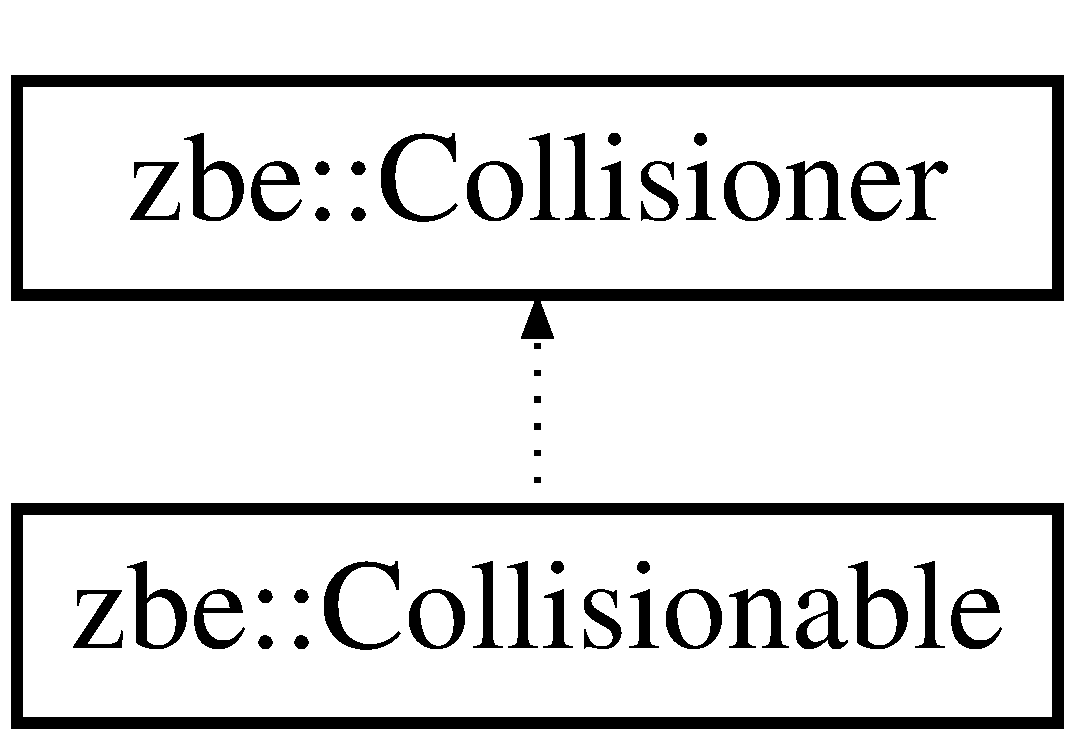
\includegraphics[height=2.000000cm]{classzbe_1_1_collisionable}
\end{center}
\end{figure}
\subsection*{Public Member Functions}
\begin{DoxyCompactItemize}
\item 
virtual \hyperlink{classzbe_1_1_collisionable_a1357e6126f1e81f8c5574535f6c60c75}{$\sim$\+Collisionable} ()
\end{DoxyCompactItemize}


\subsection{Detailed Description}


Definition at line 17 of file Collisionable.\+h.



\subsection{Constructor \& Destructor Documentation}
\hypertarget{classzbe_1_1_collisionable_a1357e6126f1e81f8c5574535f6c60c75}{}\index{zbe\+::\+Collisionable@{zbe\+::\+Collisionable}!````~Collisionable@{$\sim$\+Collisionable}}
\index{````~Collisionable@{$\sim$\+Collisionable}!zbe\+::\+Collisionable@{zbe\+::\+Collisionable}}
\subsubsection[{$\sim$\+Collisionable()}]{\setlength{\rightskip}{0pt plus 5cm}virtual zbe\+::\+Collisionable\+::$\sim$\+Collisionable (
\begin{DoxyParamCaption}
{}
\end{DoxyParamCaption}
)\hspace{0.3cm}{\ttfamily [inline]}, {\ttfamily [virtual]}}\label{classzbe_1_1_collisionable_a1357e6126f1e81f8c5574535f6c60c75}


Definition at line 19 of file Collisionable.\+h.



The documentation for this class was generated from the following file\+:\begin{DoxyCompactItemize}
\item 
include/\+Z\+B\+E/core/archetypes/\hyperlink{_collisionable_8h}{Collisionable.\+h}\end{DoxyCompactItemize}

\hypertarget{classzbe_1_1_collisionador}{}\section{zbe\+:\+:Collisionador Class Reference}
\label{classzbe_1_1_collisionador}\index{zbe\+::\+Collisionador@{zbe\+::\+Collisionador}}


{\ttfamily \#include $<$Collisionador.\+h$>$}

Inheritance diagram for zbe\+:\+:Collisionador\+:\begin{figure}[H]
\begin{center}
\leavevmode
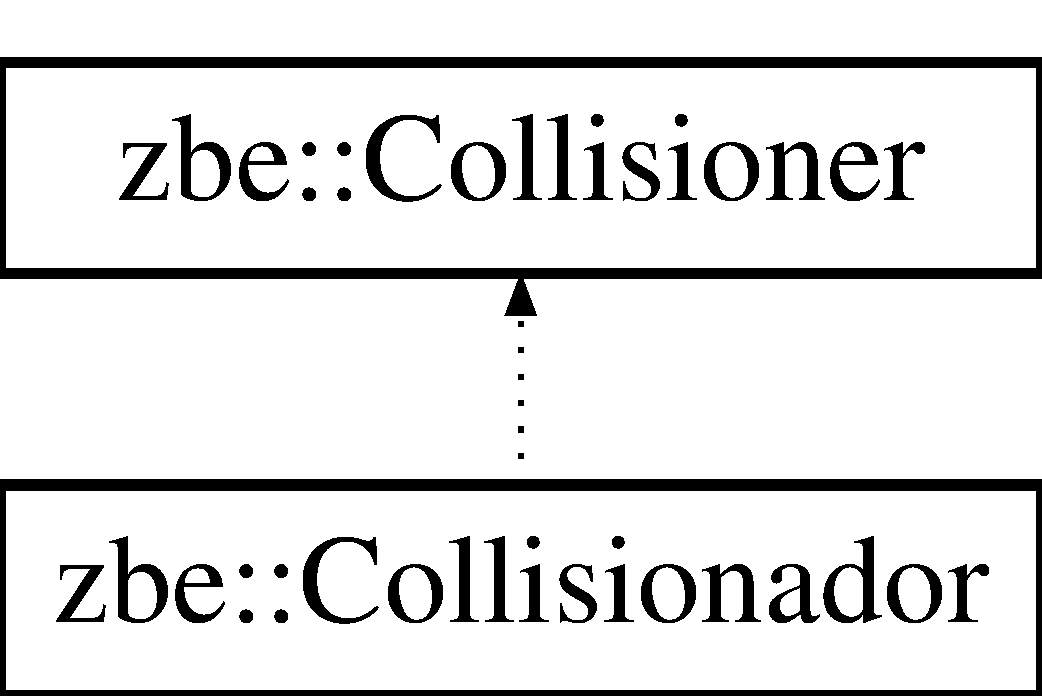
\includegraphics[height=2.000000cm]{classzbe_1_1_collisionador}
\end{center}
\end{figure}
\subsection*{Public Member Functions}
\begin{DoxyCompactItemize}
\item 
virtual \hyperlink{classzbe_1_1_collisionador_a1afd252bd30765abcc48f2f38a004400}{$\sim$\+Collisionador} ()
\item 
double \hyperlink{classzbe_1_1_collisionador_a6528a61182956a02be17a9e64af2cbed}{collision\+Detection} (std\+::forward\+\_\+list$<$ \hyperlink{classzbe_1_1_collision_data}{Collision\+Data} $>$ $\ast$cdata, double time\+Remain)
\end{DoxyCompactItemize}


\subsection{Detailed Description}


Definition at line 17 of file Collisionador.\+h.



\subsection{Constructor \& Destructor Documentation}
\hypertarget{classzbe_1_1_collisionador_a1afd252bd30765abcc48f2f38a004400}{}\index{zbe\+::\+Collisionador@{zbe\+::\+Collisionador}!````~Collisionador@{$\sim$\+Collisionador}}
\index{````~Collisionador@{$\sim$\+Collisionador}!zbe\+::\+Collisionador@{zbe\+::\+Collisionador}}
\subsubsection[{$\sim$\+Collisionador()}]{\setlength{\rightskip}{0pt plus 5cm}virtual zbe\+::\+Collisionador\+::$\sim$\+Collisionador (
\begin{DoxyParamCaption}
{}
\end{DoxyParamCaption}
)\hspace{0.3cm}{\ttfamily [inline]}, {\ttfamily [virtual]}}\label{classzbe_1_1_collisionador_a1afd252bd30765abcc48f2f38a004400}


Definition at line 19 of file Collisionador.\+h.



\subsection{Member Function Documentation}
\hypertarget{classzbe_1_1_collisionador_a6528a61182956a02be17a9e64af2cbed}{}\index{zbe\+::\+Collisionador@{zbe\+::\+Collisionador}!collision\+Detection@{collision\+Detection}}
\index{collision\+Detection@{collision\+Detection}!zbe\+::\+Collisionador@{zbe\+::\+Collisionador}}
\subsubsection[{collision\+Detection(std\+::forward\+\_\+list$<$ Collision\+Data $>$ $\ast$cdata, double time\+Remain)}]{\setlength{\rightskip}{0pt plus 5cm}double zbe\+::\+Collisionador\+::collision\+Detection (
\begin{DoxyParamCaption}
\item[{std\+::forward\+\_\+list$<$ {\bf Collision\+Data} $>$ $\ast$}]{cdata, }
\item[{double}]{time\+Remain}
\end{DoxyParamCaption}
)}\label{classzbe_1_1_collisionador_a6528a61182956a02be17a9e64af2cbed}


The documentation for this class was generated from the following file\+:\begin{DoxyCompactItemize}
\item 
include/\+Z\+B\+E/core/archetypes/\hyperlink{_collisionador_8h}{Collisionador.\+h}\end{DoxyCompactItemize}

\hypertarget{classzbe_1_1_collision_data}{}\section{zbe\+:\+:Collision\+Data Class Reference}
\label{classzbe_1_1_collision_data}\index{zbe\+::\+Collision\+Data@{zbe\+::\+Collision\+Data}}


{\ttfamily \#include $<$Collision\+Data.\+h$>$}

\subsection*{Public Member Functions}
\begin{DoxyCompactItemize}
\item 
\hyperlink{classzbe_1_1_collision_data_ada63380ed483198d18360c86bd767ab9}{Collision\+Data} (\hyperlink{classzbe_1_1_collisioner}{Collisioner} $\ast$collisionador, \hyperlink{classzbe_1_1_collisioner}{Collisioner} $\ast$collisionable, const \hyperlink{classzbe_1_1_vector2_d}{Vector2\+D} \&normal, const \hyperlink{classzbe_1_1_vector2_d}{Vector2\+D} \&point)
\item 
\hyperlink{classzbe_1_1_collisioner}{Collisioner} $\ast$ \hyperlink{classzbe_1_1_collision_data_ade8ae07a020fe3998a0b86332da2a316}{get\+Collisionador} () const 
\item 
\hyperlink{classzbe_1_1_collisioner}{Collisioner} $\ast$ \hyperlink{classzbe_1_1_collision_data_a2c7909dde4916bc03e85a5f5e7573670}{get\+Collisionable} () const 
\item 
const \hyperlink{classzbe_1_1_vector2_d}{Vector2\+D} \& \hyperlink{classzbe_1_1_collision_data_af023c2b6de52939f6a2388da30d3d6b2}{get\+Normal} () const 
\item 
const \hyperlink{classzbe_1_1_vector2_d}{Vector2\+D} \& \hyperlink{classzbe_1_1_collision_data_ac78b947b89aacd31f322d367c3348d83}{get\+Point} () const 
\item 
void \hyperlink{classzbe_1_1_collision_data_a7c80356481445bfb621413cfac43a0a4}{react} (double time)
\end{DoxyCompactItemize}


\subsection{Detailed Description}


Definition at line 18 of file Collision\+Data.\+h.



\subsection{Constructor \& Destructor Documentation}
\hypertarget{classzbe_1_1_collision_data_ada63380ed483198d18360c86bd767ab9}{}\index{zbe\+::\+Collision\+Data@{zbe\+::\+Collision\+Data}!Collision\+Data@{Collision\+Data}}
\index{Collision\+Data@{Collision\+Data}!zbe\+::\+Collision\+Data@{zbe\+::\+Collision\+Data}}
\subsubsection[{Collision\+Data(\+Collisioner $\ast$collisionador, Collisioner $\ast$collisionable, const Vector2\+D \&normal, const Vector2\+D \&point)}]{\setlength{\rightskip}{0pt plus 5cm}zbe\+::\+Collision\+Data\+::\+Collision\+Data (
\begin{DoxyParamCaption}
\item[{{\bf Collisioner} $\ast$}]{collisionador, }
\item[{{\bf Collisioner} $\ast$}]{collisionable, }
\item[{const {\bf Vector2\+D} \&}]{normal, }
\item[{const {\bf Vector2\+D} \&}]{point}
\end{DoxyParamCaption}
)\hspace{0.3cm}{\ttfamily [inline]}}\label{classzbe_1_1_collision_data_ada63380ed483198d18360c86bd767ab9}


Definition at line 20 of file Collision\+Data.\+h.



\subsection{Member Function Documentation}
\hypertarget{classzbe_1_1_collision_data_a2c7909dde4916bc03e85a5f5e7573670}{}\index{zbe\+::\+Collision\+Data@{zbe\+::\+Collision\+Data}!get\+Collisionable@{get\+Collisionable}}
\index{get\+Collisionable@{get\+Collisionable}!zbe\+::\+Collision\+Data@{zbe\+::\+Collision\+Data}}
\subsubsection[{get\+Collisionable() const }]{\setlength{\rightskip}{0pt plus 5cm}{\bf Collisioner}$\ast$ zbe\+::\+Collision\+Data\+::get\+Collisionable (
\begin{DoxyParamCaption}
{}
\end{DoxyParamCaption}
) const\hspace{0.3cm}{\ttfamily [inline]}}\label{classzbe_1_1_collision_data_a2c7909dde4916bc03e85a5f5e7573670}


Definition at line 24 of file Collision\+Data.\+h.

\hypertarget{classzbe_1_1_collision_data_ade8ae07a020fe3998a0b86332da2a316}{}\index{zbe\+::\+Collision\+Data@{zbe\+::\+Collision\+Data}!get\+Collisionador@{get\+Collisionador}}
\index{get\+Collisionador@{get\+Collisionador}!zbe\+::\+Collision\+Data@{zbe\+::\+Collision\+Data}}
\subsubsection[{get\+Collisionador() const }]{\setlength{\rightskip}{0pt plus 5cm}{\bf Collisioner}$\ast$ zbe\+::\+Collision\+Data\+::get\+Collisionador (
\begin{DoxyParamCaption}
{}
\end{DoxyParamCaption}
) const\hspace{0.3cm}{\ttfamily [inline]}}\label{classzbe_1_1_collision_data_ade8ae07a020fe3998a0b86332da2a316}


Definition at line 23 of file Collision\+Data.\+h.

\hypertarget{classzbe_1_1_collision_data_af023c2b6de52939f6a2388da30d3d6b2}{}\index{zbe\+::\+Collision\+Data@{zbe\+::\+Collision\+Data}!get\+Normal@{get\+Normal}}
\index{get\+Normal@{get\+Normal}!zbe\+::\+Collision\+Data@{zbe\+::\+Collision\+Data}}
\subsubsection[{get\+Normal() const }]{\setlength{\rightskip}{0pt plus 5cm}const {\bf Vector2\+D}\& zbe\+::\+Collision\+Data\+::get\+Normal (
\begin{DoxyParamCaption}
{}
\end{DoxyParamCaption}
) const\hspace{0.3cm}{\ttfamily [inline]}}\label{classzbe_1_1_collision_data_af023c2b6de52939f6a2388da30d3d6b2}


Definition at line 25 of file Collision\+Data.\+h.

\hypertarget{classzbe_1_1_collision_data_ac78b947b89aacd31f322d367c3348d83}{}\index{zbe\+::\+Collision\+Data@{zbe\+::\+Collision\+Data}!get\+Point@{get\+Point}}
\index{get\+Point@{get\+Point}!zbe\+::\+Collision\+Data@{zbe\+::\+Collision\+Data}}
\subsubsection[{get\+Point() const }]{\setlength{\rightskip}{0pt plus 5cm}const {\bf Vector2\+D}\& zbe\+::\+Collision\+Data\+::get\+Point (
\begin{DoxyParamCaption}
{}
\end{DoxyParamCaption}
) const\hspace{0.3cm}{\ttfamily [inline]}}\label{classzbe_1_1_collision_data_ac78b947b89aacd31f322d367c3348d83}


Definition at line 26 of file Collision\+Data.\+h.

\hypertarget{classzbe_1_1_collision_data_a7c80356481445bfb621413cfac43a0a4}{}\index{zbe\+::\+Collision\+Data@{zbe\+::\+Collision\+Data}!react@{react}}
\index{react@{react}!zbe\+::\+Collision\+Data@{zbe\+::\+Collision\+Data}}
\subsubsection[{react(double time)}]{\setlength{\rightskip}{0pt plus 5cm}void zbe\+::\+Collision\+Data\+::react (
\begin{DoxyParamCaption}
\item[{double}]{time}
\end{DoxyParamCaption}
)}\label{classzbe_1_1_collision_data_a7c80356481445bfb621413cfac43a0a4}


The documentation for this class was generated from the following file\+:\begin{DoxyCompactItemize}
\item 
include/\+Z\+B\+E/core/tools/math/collisions/\hyperlink{_collision_data_8h}{Collision\+Data.\+h}\end{DoxyCompactItemize}

\hypertarget{classzbe_1_1_collisioner}{}\section{zbe\+:\+:Collisioner Class Reference}
\label{classzbe_1_1_collisioner}\index{zbe\+::\+Collisioner@{zbe\+::\+Collisioner}}


{\ttfamily \#include $<$Collisioner.\+h$>$}

Inheritance diagram for zbe\+:\+:Collisioner\+:\begin{figure}[H]
\begin{center}
\leavevmode
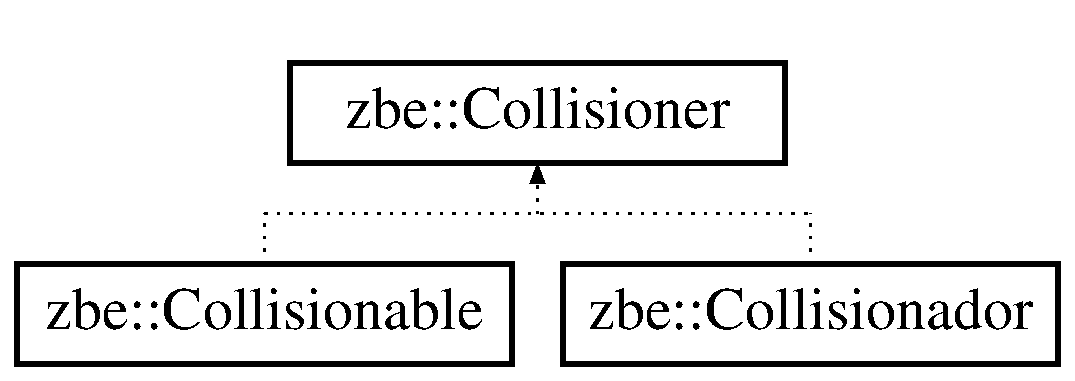
\includegraphics[height=2.000000cm]{classzbe_1_1_collisioner}
\end{center}
\end{figure}
\subsection*{Public Types}
\begin{DoxyCompactItemize}
\item 
enum \hyperlink{classzbe_1_1_collisioner_af210f5ae0183381df428b4b4f72946eb}{Collysion\+Type} \{ \hyperlink{classzbe_1_1_collisioner_af210f5ae0183381df428b4b4f72946eba65bc42fd5c16096214440f43460a4b7d}{S\+P\+H\+E\+R\+E} = 0, 
\hyperlink{classzbe_1_1_collisioner_af210f5ae0183381df428b4b4f72946ebad842cd828b17a573ed9d7d9c4f810816}{A\+A\+B\+B} = 1
 \}
\end{DoxyCompactItemize}
\subsection*{Public Member Functions}
\begin{DoxyCompactItemize}
\item 
virtual \hyperlink{classzbe_1_1_collisioner_a925d62e829a8c7d8a3589a8de01453d5}{$\sim$\+Collisioner} ()
\item 
virtual void \hyperlink{classzbe_1_1_collisioner_aee4f5ba729979c5811ab1f64689041b6}{react} (\hyperlink{classzbe_1_1_collisioner}{Collisioner} $\ast$c, const \hyperlink{classzbe_1_1_vector2_d}{Vector2\+D} \&normal, const \hyperlink{classzbe_1_1_vector2_d}{Vector2\+D} \&point, double time)=0
\item 
virtual \hyperlink{classzbe_1_1_collisioner_af210f5ae0183381df428b4b4f72946eb}{Collysion\+Type} \hyperlink{classzbe_1_1_collisioner_aa97f90d8e249f8729b283e4bcbbd8ee8}{get\+Type} ()=0
\item 
virtual unsigned \hyperlink{classzbe_1_1_collisioner_abf434f16ac9a1eceb9509c10b2ca4ec7}{collision\+Level} ()=0
\end{DoxyCompactItemize}


\subsection{Detailed Description}


Definition at line 17 of file Collisioner.\+h.



\subsection{Member Enumeration Documentation}
\hypertarget{classzbe_1_1_collisioner_af210f5ae0183381df428b4b4f72946eb}{}\index{zbe\+::\+Collisioner@{zbe\+::\+Collisioner}!Collysion\+Type@{Collysion\+Type}}
\index{Collysion\+Type@{Collysion\+Type}!zbe\+::\+Collisioner@{zbe\+::\+Collisioner}}
\subsubsection[{Collysion\+Type}]{\setlength{\rightskip}{0pt plus 5cm}enum {\bf zbe\+::\+Collisioner\+::\+Collysion\+Type}}\label{classzbe_1_1_collisioner_af210f5ae0183381df428b4b4f72946eb}
\begin{Desc}
\item[Enumerator]\par
\begin{description}
\index{S\+P\+H\+E\+R\+E@{S\+P\+H\+E\+R\+E}!zbe\+::\+Collisioner@{zbe\+::\+Collisioner}}\index{zbe\+::\+Collisioner@{zbe\+::\+Collisioner}!S\+P\+H\+E\+R\+E@{S\+P\+H\+E\+R\+E}}\item[{\em 
\hypertarget{classzbe_1_1_collisioner_af210f5ae0183381df428b4b4f72946eba65bc42fd5c16096214440f43460a4b7d}{}S\+P\+H\+E\+R\+E\label{classzbe_1_1_collisioner_af210f5ae0183381df428b4b4f72946eba65bc42fd5c16096214440f43460a4b7d}
}]\index{A\+A\+B\+B@{A\+A\+B\+B}!zbe\+::\+Collisioner@{zbe\+::\+Collisioner}}\index{zbe\+::\+Collisioner@{zbe\+::\+Collisioner}!A\+A\+B\+B@{A\+A\+B\+B}}\item[{\em 
\hypertarget{classzbe_1_1_collisioner_af210f5ae0183381df428b4b4f72946ebad842cd828b17a573ed9d7d9c4f810816}{}A\+A\+B\+B\label{classzbe_1_1_collisioner_af210f5ae0183381df428b4b4f72946ebad842cd828b17a573ed9d7d9c4f810816}
}]\end{description}
\end{Desc}


Definition at line 19 of file Collisioner.\+h.



\subsection{Constructor \& Destructor Documentation}
\hypertarget{classzbe_1_1_collisioner_a925d62e829a8c7d8a3589a8de01453d5}{}\index{zbe\+::\+Collisioner@{zbe\+::\+Collisioner}!````~Collisioner@{$\sim$\+Collisioner}}
\index{````~Collisioner@{$\sim$\+Collisioner}!zbe\+::\+Collisioner@{zbe\+::\+Collisioner}}
\subsubsection[{$\sim$\+Collisioner()}]{\setlength{\rightskip}{0pt plus 5cm}virtual zbe\+::\+Collisioner\+::$\sim$\+Collisioner (
\begin{DoxyParamCaption}
{}
\end{DoxyParamCaption}
)\hspace{0.3cm}{\ttfamily [inline]}, {\ttfamily [virtual]}}\label{classzbe_1_1_collisioner_a925d62e829a8c7d8a3589a8de01453d5}


Definition at line 24 of file Collisioner.\+h.



\subsection{Member Function Documentation}
\hypertarget{classzbe_1_1_collisioner_abf434f16ac9a1eceb9509c10b2ca4ec7}{}\index{zbe\+::\+Collisioner@{zbe\+::\+Collisioner}!collision\+Level@{collision\+Level}}
\index{collision\+Level@{collision\+Level}!zbe\+::\+Collisioner@{zbe\+::\+Collisioner}}
\subsubsection[{collision\+Level()=0}]{\setlength{\rightskip}{0pt plus 5cm}virtual unsigned zbe\+::\+Collisioner\+::collision\+Level (
\begin{DoxyParamCaption}
{}
\end{DoxyParamCaption}
)\hspace{0.3cm}{\ttfamily [pure virtual]}}\label{classzbe_1_1_collisioner_abf434f16ac9a1eceb9509c10b2ca4ec7}
\hypertarget{classzbe_1_1_collisioner_aa97f90d8e249f8729b283e4bcbbd8ee8}{}\index{zbe\+::\+Collisioner@{zbe\+::\+Collisioner}!get\+Type@{get\+Type}}
\index{get\+Type@{get\+Type}!zbe\+::\+Collisioner@{zbe\+::\+Collisioner}}
\subsubsection[{get\+Type()=0}]{\setlength{\rightskip}{0pt plus 5cm}virtual {\bf Collysion\+Type} zbe\+::\+Collisioner\+::get\+Type (
\begin{DoxyParamCaption}
{}
\end{DoxyParamCaption}
)\hspace{0.3cm}{\ttfamily [pure virtual]}}\label{classzbe_1_1_collisioner_aa97f90d8e249f8729b283e4bcbbd8ee8}
\hypertarget{classzbe_1_1_collisioner_aee4f5ba729979c5811ab1f64689041b6}{}\index{zbe\+::\+Collisioner@{zbe\+::\+Collisioner}!react@{react}}
\index{react@{react}!zbe\+::\+Collisioner@{zbe\+::\+Collisioner}}
\subsubsection[{react(\+Collisioner $\ast$c, const Vector2\+D \&normal, const Vector2\+D \&point, double time)=0}]{\setlength{\rightskip}{0pt plus 5cm}virtual void zbe\+::\+Collisioner\+::react (
\begin{DoxyParamCaption}
\item[{{\bf Collisioner} $\ast$}]{c, }
\item[{const {\bf Vector2\+D} \&}]{normal, }
\item[{const {\bf Vector2\+D} \&}]{point, }
\item[{double}]{time}
\end{DoxyParamCaption}
)\hspace{0.3cm}{\ttfamily [pure virtual]}}\label{classzbe_1_1_collisioner_aee4f5ba729979c5811ab1f64689041b6}


The documentation for this class was generated from the following file\+:\begin{DoxyCompactItemize}
\item 
include/\+Z\+B\+E/core/archetypes/\hyperlink{_collisioner_8h}{Collisioner.\+h}\end{DoxyCompactItemize}

\hypertarget{class_daemon}{}\section{Daemon Class Reference}
\label{class_daemon}\index{Daemon@{Daemon}}


{\ttfamily \#include $<$Daemon.\+h$>$}

Inheritance diagram for Daemon\+:\begin{figure}[H]
\begin{center}
\leavevmode
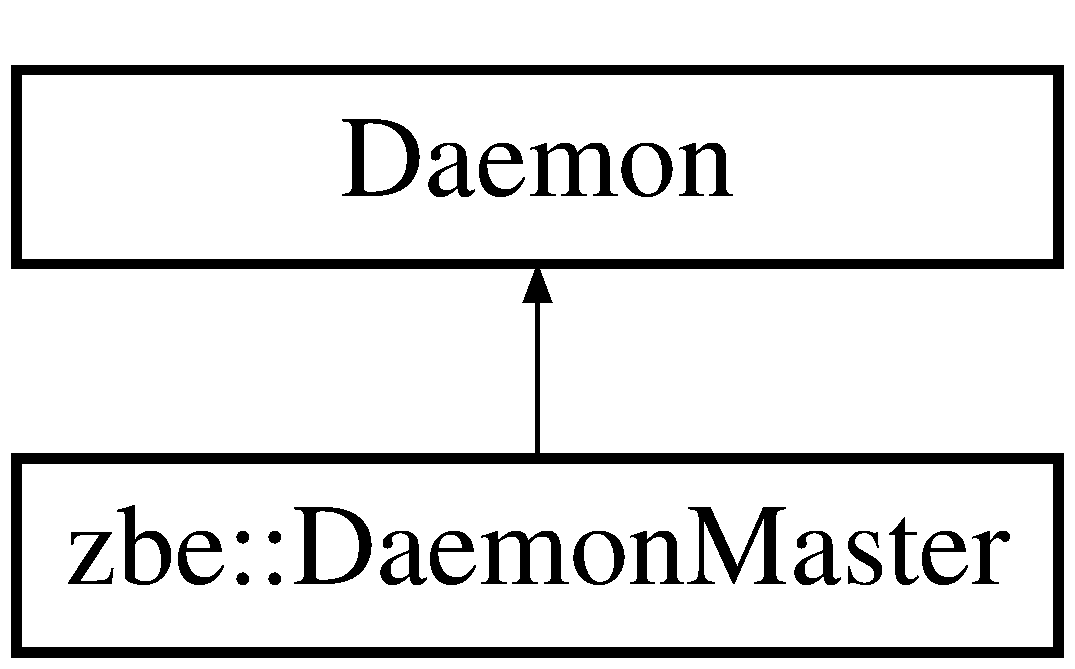
\includegraphics[height=2.000000cm]{class_daemon}
\end{center}
\end{figure}
\subsection*{Public Member Functions}
\begin{DoxyCompactItemize}
\item 
virtual void \hyperlink{class_daemon_a76c819e9805ebb2a3ec3a6d00a4a6b90}{run} ()=0
\item 
virtual \hyperlink{class_daemon_ad59d9f169a78bb4580476311bf9f246e}{$\sim$\+Daemon} ()
\end{DoxyCompactItemize}


\subsection{Detailed Description}


Definition at line 13 of file Daemon.\+h.



\subsection{Constructor \& Destructor Documentation}
\hypertarget{class_daemon_ad59d9f169a78bb4580476311bf9f246e}{}\index{Daemon@{Daemon}!````~Daemon@{$\sim$\+Daemon}}
\index{````~Daemon@{$\sim$\+Daemon}!Daemon@{Daemon}}
\subsubsection[{$\sim$\+Daemon()}]{\setlength{\rightskip}{0pt plus 5cm}virtual Daemon\+::$\sim$\+Daemon (
\begin{DoxyParamCaption}
{}
\end{DoxyParamCaption}
)\hspace{0.3cm}{\ttfamily [inline]}, {\ttfamily [virtual]}}\label{class_daemon_ad59d9f169a78bb4580476311bf9f246e}


Definition at line 16 of file Daemon.\+h.



\subsection{Member Function Documentation}
\hypertarget{class_daemon_a76c819e9805ebb2a3ec3a6d00a4a6b90}{}\index{Daemon@{Daemon}!run@{run}}
\index{run@{run}!Daemon@{Daemon}}
\subsubsection[{run()=0}]{\setlength{\rightskip}{0pt plus 5cm}virtual void Daemon\+::run (
\begin{DoxyParamCaption}
{}
\end{DoxyParamCaption}
)\hspace{0.3cm}{\ttfamily [pure virtual]}}\label{class_daemon_a76c819e9805ebb2a3ec3a6d00a4a6b90}


Implemented in \hyperlink{classzbe_1_1_daemon_master_a8e6876eb4587400f2134e5d9c7e39b73}{zbe\+::\+Daemon\+Master}.



The documentation for this class was generated from the following file\+:\begin{DoxyCompactItemize}
\item 
include/\+Z\+B\+E/core/daemons/\hyperlink{_daemon_8h}{Daemon.\+h}\end{DoxyCompactItemize}

\hypertarget{classzbe_1_1_daemon_master}{}\section{zbe\+:\+:Daemon\+Master Class Reference}
\label{classzbe_1_1_daemon_master}\index{zbe\+::\+Daemon\+Master@{zbe\+::\+Daemon\+Master}}


{\ttfamily \#include $<$Daemon\+Master.\+h$>$}

Inheritance diagram for zbe\+:\+:Daemon\+Master\+:\begin{figure}[H]
\begin{center}
\leavevmode
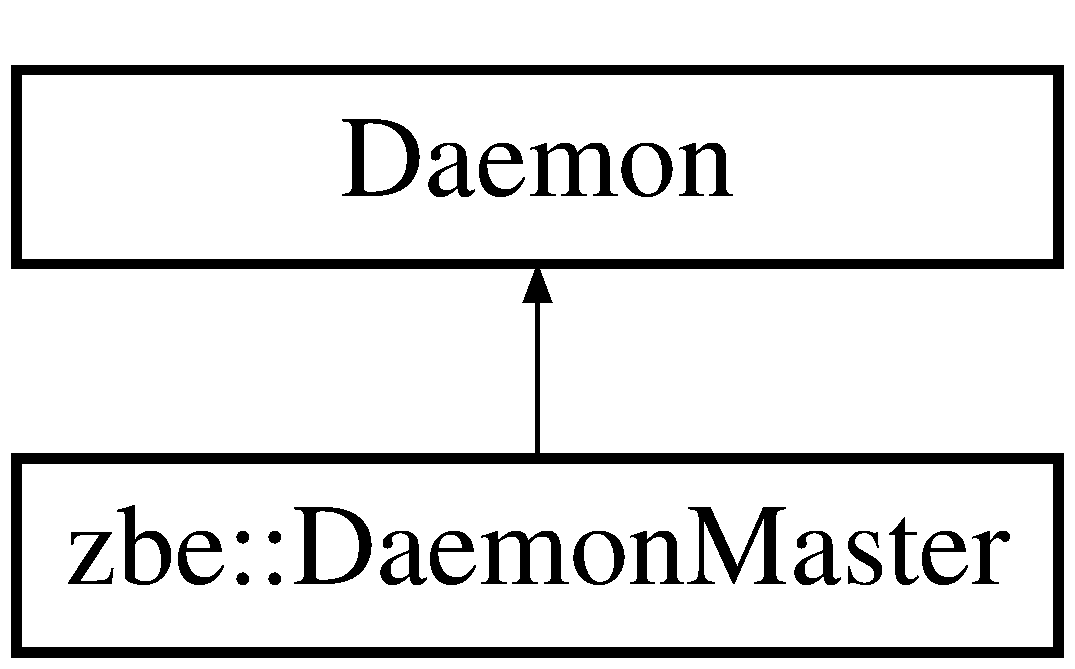
\includegraphics[height=2.000000cm]{classzbe_1_1_daemon_master}
\end{center}
\end{figure}
\subsection*{Public Member Functions}
\begin{DoxyCompactItemize}
\item 
\hyperlink{classzbe_1_1_daemon_master_abe49e03031bc2a94f5285b553cccb2dc}{Daemon\+Master} ()
\item 
virtual \hyperlink{classzbe_1_1_daemon_master_a2751a69806fd5db755f9cfb102249f7d}{$\sim$\+Daemon\+Master} ()
\item 
void \hyperlink{classzbe_1_1_daemon_master_a8e6876eb4587400f2134e5d9c7e39b73}{run} ()
\item 
void \hyperlink{classzbe_1_1_daemon_master_aa4aeee38aa6859013f7c6f5068ff1037}{add\+Daemon} (const \hyperlink{class_daemon}{Daemon} \&daemon)
\end{DoxyCompactItemize}


\subsection{Detailed Description}


Definition at line 8 of file Daemon\+Master.\+h.



\subsection{Constructor \& Destructor Documentation}
\hypertarget{classzbe_1_1_daemon_master_abe49e03031bc2a94f5285b553cccb2dc}{}\index{zbe\+::\+Daemon\+Master@{zbe\+::\+Daemon\+Master}!Daemon\+Master@{Daemon\+Master}}
\index{Daemon\+Master@{Daemon\+Master}!zbe\+::\+Daemon\+Master@{zbe\+::\+Daemon\+Master}}
\subsubsection[{Daemon\+Master()}]{\setlength{\rightskip}{0pt plus 5cm}zbe\+::\+Daemon\+Master\+::\+Daemon\+Master (
\begin{DoxyParamCaption}
{}
\end{DoxyParamCaption}
)}\label{classzbe_1_1_daemon_master_abe49e03031bc2a94f5285b553cccb2dc}
\hypertarget{classzbe_1_1_daemon_master_a2751a69806fd5db755f9cfb102249f7d}{}\index{zbe\+::\+Daemon\+Master@{zbe\+::\+Daemon\+Master}!````~Daemon\+Master@{$\sim$\+Daemon\+Master}}
\index{````~Daemon\+Master@{$\sim$\+Daemon\+Master}!zbe\+::\+Daemon\+Master@{zbe\+::\+Daemon\+Master}}
\subsubsection[{$\sim$\+Daemon\+Master()}]{\setlength{\rightskip}{0pt plus 5cm}virtual zbe\+::\+Daemon\+Master\+::$\sim$\+Daemon\+Master (
\begin{DoxyParamCaption}
{}
\end{DoxyParamCaption}
)\hspace{0.3cm}{\ttfamily [virtual]}}\label{classzbe_1_1_daemon_master_a2751a69806fd5db755f9cfb102249f7d}


\subsection{Member Function Documentation}
\hypertarget{classzbe_1_1_daemon_master_aa4aeee38aa6859013f7c6f5068ff1037}{}\index{zbe\+::\+Daemon\+Master@{zbe\+::\+Daemon\+Master}!add\+Daemon@{add\+Daemon}}
\index{add\+Daemon@{add\+Daemon}!zbe\+::\+Daemon\+Master@{zbe\+::\+Daemon\+Master}}
\subsubsection[{add\+Daemon(const Daemon \&daemon)}]{\setlength{\rightskip}{0pt plus 5cm}void zbe\+::\+Daemon\+Master\+::add\+Daemon (
\begin{DoxyParamCaption}
\item[{const {\bf Daemon} \&}]{daemon}
\end{DoxyParamCaption}
)}\label{classzbe_1_1_daemon_master_aa4aeee38aa6859013f7c6f5068ff1037}
\hypertarget{classzbe_1_1_daemon_master_a8e6876eb4587400f2134e5d9c7e39b73}{}\index{zbe\+::\+Daemon\+Master@{zbe\+::\+Daemon\+Master}!run@{run}}
\index{run@{run}!zbe\+::\+Daemon\+Master@{zbe\+::\+Daemon\+Master}}
\subsubsection[{run()}]{\setlength{\rightskip}{0pt plus 5cm}void zbe\+::\+Daemon\+Master\+::run (
\begin{DoxyParamCaption}
{}
\end{DoxyParamCaption}
)\hspace{0.3cm}{\ttfamily [virtual]}}\label{classzbe_1_1_daemon_master_a8e6876eb4587400f2134e5d9c7e39b73}


Implements \hyperlink{class_daemon_a76c819e9805ebb2a3ec3a6d00a4a6b90}{Daemon}.



The documentation for this class was generated from the following file\+:\begin{DoxyCompactItemize}
\item 
include/\+Z\+B\+E/core/daemons/\hyperlink{_daemon_master_8h}{Daemon\+Master.\+h}\end{DoxyCompactItemize}

\hypertarget{classzbe_1_1_drawer}{}\section{zbe\+:\+:Drawer Class Reference}
\label{classzbe_1_1_drawer}\index{zbe\+::\+Drawer@{zbe\+::\+Drawer}}


{\ttfamily \#include $<$Drawer.\+h$>$}

Inheritance diagram for zbe\+:\+:Drawer\+:\begin{figure}[H]
\begin{center}
\leavevmode
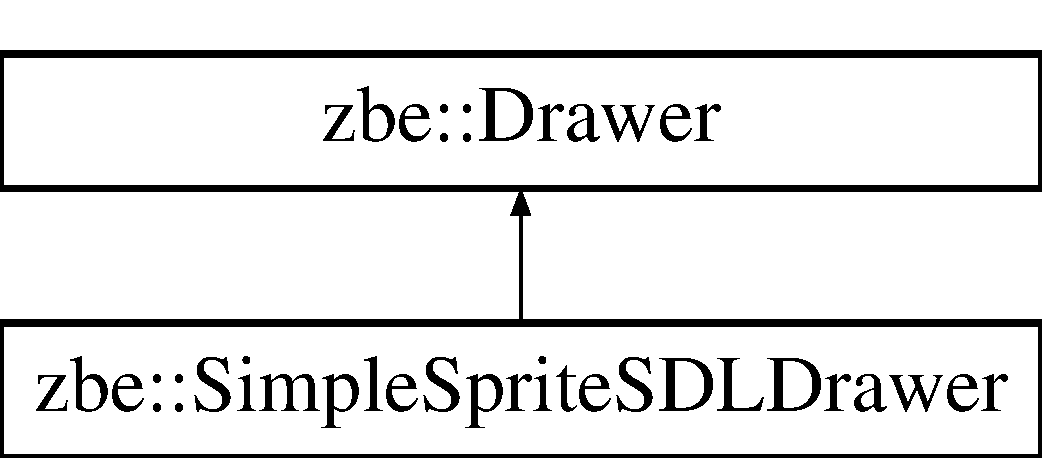
\includegraphics[height=2.000000cm]{classzbe_1_1_drawer}
\end{center}
\end{figure}
\subsection*{Public Member Functions}
\begin{DoxyCompactItemize}
\item 
virtual \hyperlink{classzbe_1_1_drawer_a1540ec7b95a19c0d6499503a74fd2062}{$\sim$\+Drawer} ()
\item 
virtual void \hyperlink{classzbe_1_1_drawer_ab890c0619125829ff83db906b1d1eb9d}{draw} ()=0
\end{DoxyCompactItemize}


\subsection{Detailed Description}


Definition at line 15 of file Drawer.\+h.



\subsection{Constructor \& Destructor Documentation}
\hypertarget{classzbe_1_1_drawer_a1540ec7b95a19c0d6499503a74fd2062}{}\index{zbe\+::\+Drawer@{zbe\+::\+Drawer}!````~Drawer@{$\sim$\+Drawer}}
\index{````~Drawer@{$\sim$\+Drawer}!zbe\+::\+Drawer@{zbe\+::\+Drawer}}
\subsubsection[{$\sim$\+Drawer()}]{\setlength{\rightskip}{0pt plus 5cm}virtual zbe\+::\+Drawer\+::$\sim$\+Drawer (
\begin{DoxyParamCaption}
{}
\end{DoxyParamCaption}
)\hspace{0.3cm}{\ttfamily [inline]}, {\ttfamily [virtual]}}\label{classzbe_1_1_drawer_a1540ec7b95a19c0d6499503a74fd2062}


Definition at line 17 of file Drawer.\+h.



\subsection{Member Function Documentation}
\hypertarget{classzbe_1_1_drawer_ab890c0619125829ff83db906b1d1eb9d}{}\index{zbe\+::\+Drawer@{zbe\+::\+Drawer}!draw@{draw}}
\index{draw@{draw}!zbe\+::\+Drawer@{zbe\+::\+Drawer}}
\subsubsection[{draw()=0}]{\setlength{\rightskip}{0pt plus 5cm}virtual void zbe\+::\+Drawer\+::draw (
\begin{DoxyParamCaption}
{}
\end{DoxyParamCaption}
)\hspace{0.3cm}{\ttfamily [pure virtual]}}\label{classzbe_1_1_drawer_ab890c0619125829ff83db906b1d1eb9d}


Implemented in \hyperlink{classzbe_1_1_simple_sprite_s_d_l_drawer_af807a5376aafaa13dce5b8e8edf3973b}{zbe\+::\+Simple\+Sprite\+S\+D\+L\+Drawer}.



The documentation for this class was generated from the following file\+:\begin{DoxyCompactItemize}
\item 
include/\+Z\+B\+E/core/drawers/\hyperlink{_drawer_8h}{Drawer.\+h}\end{DoxyCompactItemize}

\hypertarget{classzbe_1_1_file_handler}{}\section{zbe\+:\+:File\+Handler Class Reference}
\label{classzbe_1_1_file_handler}\index{zbe\+::\+File\+Handler@{zbe\+::\+File\+Handler}}


{\ttfamily \#include $<$File\+Handler.\+h$>$}

\subsection*{Public Member Functions}
\begin{DoxyCompactItemize}
\item 
\hyperlink{classzbe_1_1_file_handler_afd7d7207a3bfc6295dde9a478c77b0e5}{File\+Handler} (const char $\ast$filename, const char $\ast$mode, bool create\+Path=false)
\item 
\hyperlink{classzbe_1_1_file_handler_a48d9b38cf1de51c80e990f3b0f2e79f4}{$\sim$\+File\+Handler} ()
\item 
size\+\_\+t \hyperlink{classzbe_1_1_file_handler_a3410ba3e6b68c848a7da77aec020cc32}{read} (void $\ast$buffer, size\+\_\+t size, size\+\_\+t count)
\item 
char $\ast$ \hyperlink{classzbe_1_1_file_handler_a8a1f0e0239e0876a665fd7bc0f6c5334}{readln} (char $\ast$buffer, size\+\_\+t size)
\item 
size\+\_\+t \hyperlink{classzbe_1_1_file_handler_acdb16ed40cd778f23d1d1246ffce47c9}{write} (const char $\ast$text)
\item 
size\+\_\+t \hyperlink{classzbe_1_1_file_handler_a43df606f64a33c739973d27ee246ed2f}{write} (const void $\ast$buffer, size\+\_\+t size, size\+\_\+t count)
\item 
size\+\_\+t \hyperlink{classzbe_1_1_file_handler_a7b929b91cb770dda64367135ef572369}{writeflush} (const char $\ast$text)
\item 
size\+\_\+t \hyperlink{classzbe_1_1_file_handler_adee1df5194be8d59da5fe821d1270991}{writeflush} (const void $\ast$buffer, size\+\_\+t size, size\+\_\+t count)
\item 
size\+\_\+t \hyperlink{classzbe_1_1_file_handler_ab1f25f337fa383209d8ed8f9c6421e95}{writeln} (const char $\ast$text)
\item 
size\+\_\+t \hyperlink{classzbe_1_1_file_handler_a47a02501308c7d7ec86bae4079f8b779}{writeln} (const void $\ast$buffer, size\+\_\+t size, size\+\_\+t count)
\item 
size\+\_\+t \hyperlink{classzbe_1_1_file_handler_a09ec7d2128ef86f67333e9dd3a693ac4}{writelnflush} (const char $\ast$text)
\item 
size\+\_\+t \hyperlink{classzbe_1_1_file_handler_addc9aed59f56b5f26bb35feb5db2c632}{writelnflush} (const void $\ast$buffer, size\+\_\+t size, size\+\_\+t count)
\item 
void \hyperlink{classzbe_1_1_file_handler_aed585d5a4fd962bcaa350c915dd69e6f}{flush} ()
\end{DoxyCompactItemize}
\subsection*{Static Public Member Functions}
\begin{DoxyCompactItemize}
\item 
static bool \hyperlink{classzbe_1_1_file_handler_afc0c99ba07d653671d271fe6000c772f}{exist} (const char $\ast$filename)
\item 
static bool \hyperlink{classzbe_1_1_file_handler_a0085b4c9f3f694a61d2bca1ebf8e4e66}{exist\+Dir} (const char $\ast$filename)
\item 
static int \hyperlink{classzbe_1_1_file_handler_ade168a7f9351c88f053095e7f543e467}{rm} (const char $\ast$filename)
\item 
static bool \hyperlink{classzbe_1_1_file_handler_a7a84525a79079d436e1ee2b0ce532433}{rmdir} (const char $\ast$filename)
\end{DoxyCompactItemize}


\subsection{Detailed Description}


Definition at line 26 of file File\+Handler.\+h.



\subsection{Constructor \& Destructor Documentation}
\hypertarget{classzbe_1_1_file_handler_afd7d7207a3bfc6295dde9a478c77b0e5}{}\index{zbe\+::\+File\+Handler@{zbe\+::\+File\+Handler}!File\+Handler@{File\+Handler}}
\index{File\+Handler@{File\+Handler}!zbe\+::\+File\+Handler@{zbe\+::\+File\+Handler}}
\subsubsection[{File\+Handler(const char $\ast$filename, const char $\ast$mode, bool create\+Path=false)}]{\setlength{\rightskip}{0pt plus 5cm}zbe\+::\+File\+Handler\+::\+File\+Handler (
\begin{DoxyParamCaption}
\item[{const char $\ast$}]{filename, }
\item[{const char $\ast$}]{mode, }
\item[{bool}]{create\+Path = {\ttfamily false}}
\end{DoxyParamCaption}
)}\label{classzbe_1_1_file_handler_afd7d7207a3bfc6295dde9a478c77b0e5}
\hypertarget{classzbe_1_1_file_handler_a48d9b38cf1de51c80e990f3b0f2e79f4}{}\index{zbe\+::\+File\+Handler@{zbe\+::\+File\+Handler}!````~File\+Handler@{$\sim$\+File\+Handler}}
\index{````~File\+Handler@{$\sim$\+File\+Handler}!zbe\+::\+File\+Handler@{zbe\+::\+File\+Handler}}
\subsubsection[{$\sim$\+File\+Handler()}]{\setlength{\rightskip}{0pt plus 5cm}zbe\+::\+File\+Handler\+::$\sim$\+File\+Handler (
\begin{DoxyParamCaption}
{}
\end{DoxyParamCaption}
)}\label{classzbe_1_1_file_handler_a48d9b38cf1de51c80e990f3b0f2e79f4}


\subsection{Member Function Documentation}
\hypertarget{classzbe_1_1_file_handler_afc0c99ba07d653671d271fe6000c772f}{}\index{zbe\+::\+File\+Handler@{zbe\+::\+File\+Handler}!exist@{exist}}
\index{exist@{exist}!zbe\+::\+File\+Handler@{zbe\+::\+File\+Handler}}
\subsubsection[{exist(const char $\ast$filename)}]{\setlength{\rightskip}{0pt plus 5cm}static bool zbe\+::\+File\+Handler\+::exist (
\begin{DoxyParamCaption}
\item[{const char $\ast$}]{filename}
\end{DoxyParamCaption}
)\hspace{0.3cm}{\ttfamily [static]}}\label{classzbe_1_1_file_handler_afc0c99ba07d653671d271fe6000c772f}
\hypertarget{classzbe_1_1_file_handler_a0085b4c9f3f694a61d2bca1ebf8e4e66}{}\index{zbe\+::\+File\+Handler@{zbe\+::\+File\+Handler}!exist\+Dir@{exist\+Dir}}
\index{exist\+Dir@{exist\+Dir}!zbe\+::\+File\+Handler@{zbe\+::\+File\+Handler}}
\subsubsection[{exist\+Dir(const char $\ast$filename)}]{\setlength{\rightskip}{0pt plus 5cm}static bool zbe\+::\+File\+Handler\+::exist\+Dir (
\begin{DoxyParamCaption}
\item[{const char $\ast$}]{filename}
\end{DoxyParamCaption}
)\hspace{0.3cm}{\ttfamily [static]}}\label{classzbe_1_1_file_handler_a0085b4c9f3f694a61d2bca1ebf8e4e66}
\hypertarget{classzbe_1_1_file_handler_aed585d5a4fd962bcaa350c915dd69e6f}{}\index{zbe\+::\+File\+Handler@{zbe\+::\+File\+Handler}!flush@{flush}}
\index{flush@{flush}!zbe\+::\+File\+Handler@{zbe\+::\+File\+Handler}}
\subsubsection[{flush()}]{\setlength{\rightskip}{0pt plus 5cm}void zbe\+::\+File\+Handler\+::flush (
\begin{DoxyParamCaption}
{}
\end{DoxyParamCaption}
)}\label{classzbe_1_1_file_handler_aed585d5a4fd962bcaa350c915dd69e6f}
\hypertarget{classzbe_1_1_file_handler_a3410ba3e6b68c848a7da77aec020cc32}{}\index{zbe\+::\+File\+Handler@{zbe\+::\+File\+Handler}!read@{read}}
\index{read@{read}!zbe\+::\+File\+Handler@{zbe\+::\+File\+Handler}}
\subsubsection[{read(void $\ast$buffer, size\+\_\+t size, size\+\_\+t count)}]{\setlength{\rightskip}{0pt plus 5cm}size\+\_\+t zbe\+::\+File\+Handler\+::read (
\begin{DoxyParamCaption}
\item[{void $\ast$}]{buffer, }
\item[{size\+\_\+t}]{size, }
\item[{size\+\_\+t}]{count}
\end{DoxyParamCaption}
)}\label{classzbe_1_1_file_handler_a3410ba3e6b68c848a7da77aec020cc32}
\hypertarget{classzbe_1_1_file_handler_a8a1f0e0239e0876a665fd7bc0f6c5334}{}\index{zbe\+::\+File\+Handler@{zbe\+::\+File\+Handler}!readln@{readln}}
\index{readln@{readln}!zbe\+::\+File\+Handler@{zbe\+::\+File\+Handler}}
\subsubsection[{readln(char $\ast$buffer, size\+\_\+t size)}]{\setlength{\rightskip}{0pt plus 5cm}char$\ast$ zbe\+::\+File\+Handler\+::readln (
\begin{DoxyParamCaption}
\item[{char $\ast$}]{buffer, }
\item[{size\+\_\+t}]{size}
\end{DoxyParamCaption}
)}\label{classzbe_1_1_file_handler_a8a1f0e0239e0876a665fd7bc0f6c5334}
\hypertarget{classzbe_1_1_file_handler_ade168a7f9351c88f053095e7f543e467}{}\index{zbe\+::\+File\+Handler@{zbe\+::\+File\+Handler}!rm@{rm}}
\index{rm@{rm}!zbe\+::\+File\+Handler@{zbe\+::\+File\+Handler}}
\subsubsection[{rm(const char $\ast$filename)}]{\setlength{\rightskip}{0pt plus 5cm}static int zbe\+::\+File\+Handler\+::rm (
\begin{DoxyParamCaption}
\item[{const char $\ast$}]{filename}
\end{DoxyParamCaption}
)\hspace{0.3cm}{\ttfamily [static]}}\label{classzbe_1_1_file_handler_ade168a7f9351c88f053095e7f543e467}
\hypertarget{classzbe_1_1_file_handler_a7a84525a79079d436e1ee2b0ce532433}{}\index{zbe\+::\+File\+Handler@{zbe\+::\+File\+Handler}!rmdir@{rmdir}}
\index{rmdir@{rmdir}!zbe\+::\+File\+Handler@{zbe\+::\+File\+Handler}}
\subsubsection[{rmdir(const char $\ast$filename)}]{\setlength{\rightskip}{0pt plus 5cm}static bool zbe\+::\+File\+Handler\+::rmdir (
\begin{DoxyParamCaption}
\item[{const char $\ast$}]{filename}
\end{DoxyParamCaption}
)\hspace{0.3cm}{\ttfamily [static]}}\label{classzbe_1_1_file_handler_a7a84525a79079d436e1ee2b0ce532433}
\hypertarget{classzbe_1_1_file_handler_acdb16ed40cd778f23d1d1246ffce47c9}{}\index{zbe\+::\+File\+Handler@{zbe\+::\+File\+Handler}!write@{write}}
\index{write@{write}!zbe\+::\+File\+Handler@{zbe\+::\+File\+Handler}}
\subsubsection[{write(const char $\ast$text)}]{\setlength{\rightskip}{0pt plus 5cm}size\+\_\+t zbe\+::\+File\+Handler\+::write (
\begin{DoxyParamCaption}
\item[{const char $\ast$}]{text}
\end{DoxyParamCaption}
)}\label{classzbe_1_1_file_handler_acdb16ed40cd778f23d1d1246ffce47c9}
\hypertarget{classzbe_1_1_file_handler_a43df606f64a33c739973d27ee246ed2f}{}\index{zbe\+::\+File\+Handler@{zbe\+::\+File\+Handler}!write@{write}}
\index{write@{write}!zbe\+::\+File\+Handler@{zbe\+::\+File\+Handler}}
\subsubsection[{write(const void $\ast$buffer, size\+\_\+t size, size\+\_\+t count)}]{\setlength{\rightskip}{0pt plus 5cm}size\+\_\+t zbe\+::\+File\+Handler\+::write (
\begin{DoxyParamCaption}
\item[{const void $\ast$}]{buffer, }
\item[{size\+\_\+t}]{size, }
\item[{size\+\_\+t}]{count}
\end{DoxyParamCaption}
)}\label{classzbe_1_1_file_handler_a43df606f64a33c739973d27ee246ed2f}
\hypertarget{classzbe_1_1_file_handler_a7b929b91cb770dda64367135ef572369}{}\index{zbe\+::\+File\+Handler@{zbe\+::\+File\+Handler}!writeflush@{writeflush}}
\index{writeflush@{writeflush}!zbe\+::\+File\+Handler@{zbe\+::\+File\+Handler}}
\subsubsection[{writeflush(const char $\ast$text)}]{\setlength{\rightskip}{0pt plus 5cm}size\+\_\+t zbe\+::\+File\+Handler\+::writeflush (
\begin{DoxyParamCaption}
\item[{const char $\ast$}]{text}
\end{DoxyParamCaption}
)}\label{classzbe_1_1_file_handler_a7b929b91cb770dda64367135ef572369}
\hypertarget{classzbe_1_1_file_handler_adee1df5194be8d59da5fe821d1270991}{}\index{zbe\+::\+File\+Handler@{zbe\+::\+File\+Handler}!writeflush@{writeflush}}
\index{writeflush@{writeflush}!zbe\+::\+File\+Handler@{zbe\+::\+File\+Handler}}
\subsubsection[{writeflush(const void $\ast$buffer, size\+\_\+t size, size\+\_\+t count)}]{\setlength{\rightskip}{0pt plus 5cm}size\+\_\+t zbe\+::\+File\+Handler\+::writeflush (
\begin{DoxyParamCaption}
\item[{const void $\ast$}]{buffer, }
\item[{size\+\_\+t}]{size, }
\item[{size\+\_\+t}]{count}
\end{DoxyParamCaption}
)}\label{classzbe_1_1_file_handler_adee1df5194be8d59da5fe821d1270991}
\hypertarget{classzbe_1_1_file_handler_ab1f25f337fa383209d8ed8f9c6421e95}{}\index{zbe\+::\+File\+Handler@{zbe\+::\+File\+Handler}!writeln@{writeln}}
\index{writeln@{writeln}!zbe\+::\+File\+Handler@{zbe\+::\+File\+Handler}}
\subsubsection[{writeln(const char $\ast$text)}]{\setlength{\rightskip}{0pt plus 5cm}size\+\_\+t zbe\+::\+File\+Handler\+::writeln (
\begin{DoxyParamCaption}
\item[{const char $\ast$}]{text}
\end{DoxyParamCaption}
)}\label{classzbe_1_1_file_handler_ab1f25f337fa383209d8ed8f9c6421e95}
\hypertarget{classzbe_1_1_file_handler_a47a02501308c7d7ec86bae4079f8b779}{}\index{zbe\+::\+File\+Handler@{zbe\+::\+File\+Handler}!writeln@{writeln}}
\index{writeln@{writeln}!zbe\+::\+File\+Handler@{zbe\+::\+File\+Handler}}
\subsubsection[{writeln(const void $\ast$buffer, size\+\_\+t size, size\+\_\+t count)}]{\setlength{\rightskip}{0pt plus 5cm}size\+\_\+t zbe\+::\+File\+Handler\+::writeln (
\begin{DoxyParamCaption}
\item[{const void $\ast$}]{buffer, }
\item[{size\+\_\+t}]{size, }
\item[{size\+\_\+t}]{count}
\end{DoxyParamCaption}
)}\label{classzbe_1_1_file_handler_a47a02501308c7d7ec86bae4079f8b779}
\hypertarget{classzbe_1_1_file_handler_a09ec7d2128ef86f67333e9dd3a693ac4}{}\index{zbe\+::\+File\+Handler@{zbe\+::\+File\+Handler}!writelnflush@{writelnflush}}
\index{writelnflush@{writelnflush}!zbe\+::\+File\+Handler@{zbe\+::\+File\+Handler}}
\subsubsection[{writelnflush(const char $\ast$text)}]{\setlength{\rightskip}{0pt plus 5cm}size\+\_\+t zbe\+::\+File\+Handler\+::writelnflush (
\begin{DoxyParamCaption}
\item[{const char $\ast$}]{text}
\end{DoxyParamCaption}
)}\label{classzbe_1_1_file_handler_a09ec7d2128ef86f67333e9dd3a693ac4}
\hypertarget{classzbe_1_1_file_handler_addc9aed59f56b5f26bb35feb5db2c632}{}\index{zbe\+::\+File\+Handler@{zbe\+::\+File\+Handler}!writelnflush@{writelnflush}}
\index{writelnflush@{writelnflush}!zbe\+::\+File\+Handler@{zbe\+::\+File\+Handler}}
\subsubsection[{writelnflush(const void $\ast$buffer, size\+\_\+t size, size\+\_\+t count)}]{\setlength{\rightskip}{0pt plus 5cm}size\+\_\+t zbe\+::\+File\+Handler\+::writelnflush (
\begin{DoxyParamCaption}
\item[{const void $\ast$}]{buffer, }
\item[{size\+\_\+t}]{size, }
\item[{size\+\_\+t}]{count}
\end{DoxyParamCaption}
)}\label{classzbe_1_1_file_handler_addc9aed59f56b5f26bb35feb5db2c632}


The documentation for this class was generated from the following file\+:\begin{DoxyCompactItemize}
\item 
include/\+Z\+B\+E/core/io/\hyperlink{_file_handler_8h}{File\+Handler.\+h}\end{DoxyCompactItemize}

\hypertarget{classzbe_1_1_game_app}{}\section{zbe\+:\+:Game\+App Class Reference}
\label{classzbe_1_1_game_app}\index{zbe\+::\+Game\+App@{zbe\+::\+Game\+App}}


{\ttfamily \#include $<$Game\+App.\+h$>$}

Inheritance diagram for zbe\+:\+:Game\+App\+:\begin{figure}[H]
\begin{center}
\leavevmode
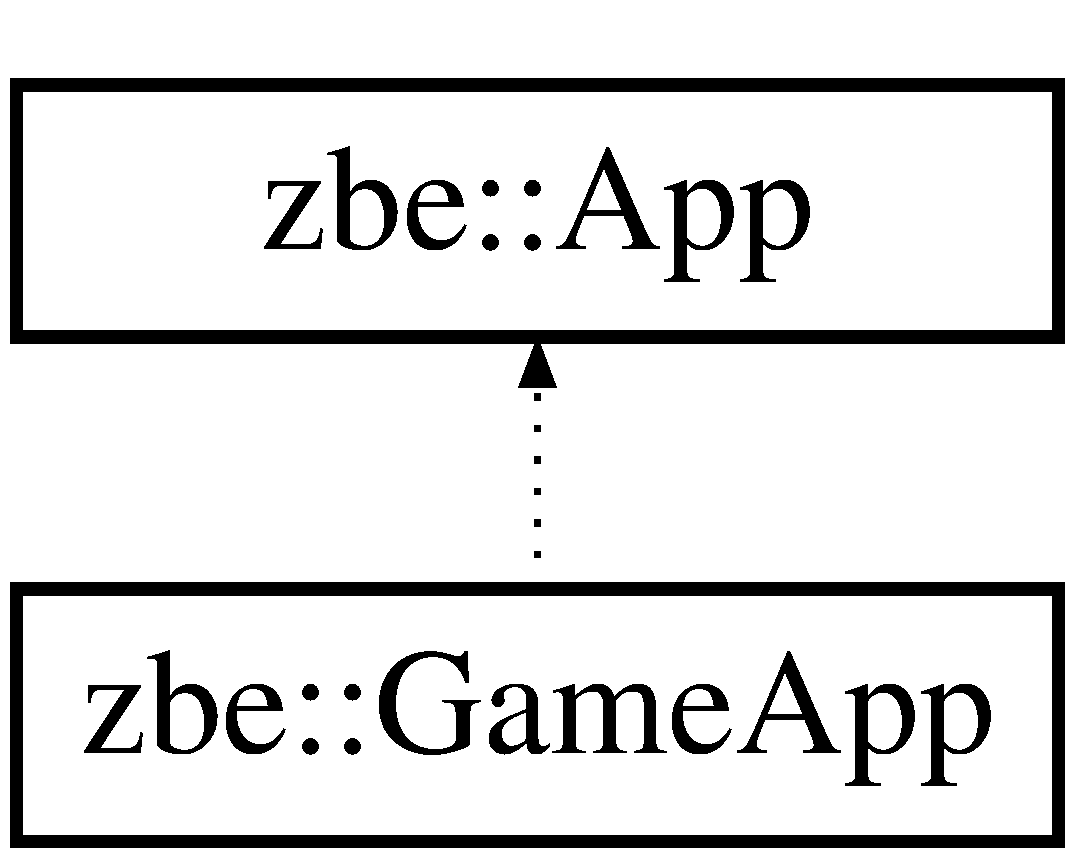
\includegraphics[height=2.000000cm]{classzbe_1_1_game_app}
\end{center}
\end{figure}
\subsection*{Public Member Functions}
\begin{DoxyCompactItemize}
\item 
virtual \hyperlink{classzbe_1_1_game_app_aa022d099e2c8e7937dd44fa15250b08e}{$\sim$\+Game\+App} ()
\item 
void \hyperlink{classzbe_1_1_game_app_ae392423ebb0a09e9505889efff180dca}{behavevior\+And\+Physics} ()
\item 
void \hyperlink{classzbe_1_1_game_app_a15f835d8a2ddacb5b521fa2235f77b94}{behave\+Until} (double time)
\item 
void \hyperlink{classzbe_1_1_game_app_aa78afb55a2eff504e40288bc0aef6d65}{draw} ()
\end{DoxyCompactItemize}
\subsection*{Protected Member Functions}
\begin{DoxyCompactItemize}
\item 
double \hyperlink{classzbe_1_1_game_app_a900a7f2dfa48b901bc9c8dc9dc196b79}{collision\+Detection} (std\+::forward\+\_\+list$<$ \hyperlink{classzbe_1_1_collision_data}{Collision\+Data} $>$ $\ast$cdata, double time\+Remain)
\item 
void \hyperlink{classzbe_1_1_game_app_a25d5110ddc958af4673790c1b2b7396e}{report\+Collision} (const std\+::forward\+\_\+list$<$ \hyperlink{classzbe_1_1_collision_data}{Collision\+Data} $>$ \&cdata, double collision\+Time)
\end{DoxyCompactItemize}


\subsection{Detailed Description}


Definition at line 48 of file Game\+App.\+h.



\subsection{Constructor \& Destructor Documentation}
\hypertarget{classzbe_1_1_game_app_aa022d099e2c8e7937dd44fa15250b08e}{}\index{zbe\+::\+Game\+App@{zbe\+::\+Game\+App}!````~Game\+App@{$\sim$\+Game\+App}}
\index{````~Game\+App@{$\sim$\+Game\+App}!zbe\+::\+Game\+App@{zbe\+::\+Game\+App}}
\subsubsection[{$\sim$\+Game\+App()}]{\setlength{\rightskip}{0pt plus 5cm}virtual zbe\+::\+Game\+App\+::$\sim$\+Game\+App (
\begin{DoxyParamCaption}
{}
\end{DoxyParamCaption}
)\hspace{0.3cm}{\ttfamily [inline]}, {\ttfamily [virtual]}}\label{classzbe_1_1_game_app_aa022d099e2c8e7937dd44fa15250b08e}


Definition at line 50 of file Game\+App.\+h.



\subsection{Member Function Documentation}
\hypertarget{classzbe_1_1_game_app_a15f835d8a2ddacb5b521fa2235f77b94}{}\index{zbe\+::\+Game\+App@{zbe\+::\+Game\+App}!behave\+Until@{behave\+Until}}
\index{behave\+Until@{behave\+Until}!zbe\+::\+Game\+App@{zbe\+::\+Game\+App}}
\subsubsection[{behave\+Until(double time)}]{\setlength{\rightskip}{0pt plus 5cm}void zbe\+::\+Game\+App\+::behave\+Until (
\begin{DoxyParamCaption}
\item[{double}]{time}
\end{DoxyParamCaption}
)}\label{classzbe_1_1_game_app_a15f835d8a2ddacb5b521fa2235f77b94}


Definition at line 88 of file Game\+App.\+h.

\hypertarget{classzbe_1_1_game_app_ae392423ebb0a09e9505889efff180dca}{}\index{zbe\+::\+Game\+App@{zbe\+::\+Game\+App}!behavevior\+And\+Physics@{behavevior\+And\+Physics}}
\index{behavevior\+And\+Physics@{behavevior\+And\+Physics}!zbe\+::\+Game\+App@{zbe\+::\+Game\+App}}
\subsubsection[{behavevior\+And\+Physics()}]{\setlength{\rightskip}{0pt plus 5cm}void zbe\+::\+Game\+App\+::behavevior\+And\+Physics (
\begin{DoxyParamCaption}
{}
\end{DoxyParamCaption}
)}\label{classzbe_1_1_game_app_ae392423ebb0a09e9505889efff180dca}


Definition at line 74 of file Game\+App.\+h.

\hypertarget{classzbe_1_1_game_app_a900a7f2dfa48b901bc9c8dc9dc196b79}{}\index{zbe\+::\+Game\+App@{zbe\+::\+Game\+App}!collision\+Detection@{collision\+Detection}}
\index{collision\+Detection@{collision\+Detection}!zbe\+::\+Game\+App@{zbe\+::\+Game\+App}}
\subsubsection[{collision\+Detection(std\+::forward\+\_\+list$<$ Collision\+Data $>$ $\ast$cdata, double time\+Remain)}]{\setlength{\rightskip}{0pt plus 5cm}double zbe\+::\+Game\+App\+::collision\+Detection (
\begin{DoxyParamCaption}
\item[{std\+::forward\+\_\+list$<$ {\bf Collision\+Data} $>$ $\ast$}]{cdata, }
\item[{double}]{time\+Remain}
\end{DoxyParamCaption}
)\hspace{0.3cm}{\ttfamily [protected]}}\label{classzbe_1_1_game_app_a900a7f2dfa48b901bc9c8dc9dc196b79}


Definition at line 94 of file Game\+App.\+h.

\hypertarget{classzbe_1_1_game_app_aa78afb55a2eff504e40288bc0aef6d65}{}\index{zbe\+::\+Game\+App@{zbe\+::\+Game\+App}!draw@{draw}}
\index{draw@{draw}!zbe\+::\+Game\+App@{zbe\+::\+Game\+App}}
\subsubsection[{draw()}]{\setlength{\rightskip}{0pt plus 5cm}void zbe\+::\+Game\+App\+::draw (
\begin{DoxyParamCaption}
{}
\end{DoxyParamCaption}
)}\label{classzbe_1_1_game_app_aa78afb55a2eff504e40288bc0aef6d65}
\hypertarget{classzbe_1_1_game_app_a25d5110ddc958af4673790c1b2b7396e}{}\index{zbe\+::\+Game\+App@{zbe\+::\+Game\+App}!report\+Collision@{report\+Collision}}
\index{report\+Collision@{report\+Collision}!zbe\+::\+Game\+App@{zbe\+::\+Game\+App}}
\subsubsection[{report\+Collision(const std\+::forward\+\_\+list$<$ Collision\+Data $>$ \&cdata, double collision\+Time)}]{\setlength{\rightskip}{0pt plus 5cm}void zbe\+::\+Game\+App\+::report\+Collision (
\begin{DoxyParamCaption}
\item[{const std\+::forward\+\_\+list$<$ {\bf Collision\+Data} $>$ \&}]{cdata, }
\item[{double}]{collision\+Time}
\end{DoxyParamCaption}
)\hspace{0.3cm}{\ttfamily [protected]}}\label{classzbe_1_1_game_app_a25d5110ddc958af4673790c1b2b7396e}


Definition at line 103 of file Game\+App.\+h.



The documentation for this class was generated from the following file\+:\begin{DoxyCompactItemize}
\item 
include/\+Z\+B\+E/core/system/\hyperlink{_game_app_8h}{Game\+App.\+h}\end{DoxyCompactItemize}

\hypertarget{classzbe_1_1_logger}{}\section{zbe\+:\+:Logger Class Reference}
\label{classzbe_1_1_logger}\index{zbe\+::\+Logger@{zbe\+::\+Logger}}


A class to handle logs.  




{\ttfamily \#include $<$Logger.\+h$>$}

\subsection*{Public Types}
\begin{DoxyCompactItemize}
\item 
using \hyperlink{classzbe_1_1_logger_a6b5096e1cd8e8af221619572797cc838}{Writer\+Callback} = void($\ast$)(int ntype, const char $\ast$msgtype, const char $\ast$msg)
\begin{DoxyCompactList}\small\item\em Define a user defined writer to use with the \hyperlink{classzbe_1_1_logger}{Logger}. \end{DoxyCompactList}\end{DoxyCompactItemize}
\subsection*{Public Member Functions}
\begin{DoxyCompactItemize}
\item 
void \hyperlink{classzbe_1_1_logger_a9f8153d2ff5de8545989862aec26756b}{set\+Default\+File\+Writer} ()
\begin{DoxyCompactList}\small\item\em Add a file writer to the \hyperlink{classzbe_1_1_logger}{Logger}. \end{DoxyCompactList}\item 
void \hyperlink{classzbe_1_1_logger_a799c5a801abd4851abcd809d6ef988e3}{set\+Default\+Command\+Line\+Writer} ()
\begin{DoxyCompactList}\small\item\em Add a command line writer to the \hyperlink{classzbe_1_1_logger}{Logger}. \end{DoxyCompactList}\item 
void \hyperlink{classzbe_1_1_logger_a9385884e177d21ed09623f52500ef1b1}{set\+Default\+Writers} ()
\begin{DoxyCompactList}\small\item\em Add a file and command line writers to the \hyperlink{classzbe_1_1_logger}{Logger}. \end{DoxyCompactList}\item 
void \hyperlink{classzbe_1_1_logger_a239d4a3b868b12cccb0f88b5aa06b6a8}{add\+Writer} (\hyperlink{classzbe_1_1_logger_a6b5096e1cd8e8af221619572797cc838}{Writer\+Callback} callback)
\begin{DoxyCompactList}\small\item\em Add a user defined writer to the \hyperlink{classzbe_1_1_logger}{Logger}. \end{DoxyCompactList}\item 
void \hyperlink{classzbe_1_1_logger_af4f5d604d20ead87b807e41cdf323bc6}{log} (int ntype, const char $\ast$msgtype, \hyperlink{classzbe_1_1_logger_msg}{Logger\+Msg} msg)
\begin{DoxyCompactList}\small\item\em Log a new annotation. \end{DoxyCompactList}\end{DoxyCompactItemize}
\subsection*{Static Public Member Functions}
\begin{DoxyCompactItemize}
\item 
static \hyperlink{classzbe_1_1_logger}{Logger} $\ast$ \hyperlink{classzbe_1_1_logger_a7b2bb1e235789bfdb3a316855c8437f5}{create\+Instance} ()
\begin{DoxyCompactList}\small\item\em Create the \hyperlink{classzbe_1_1_logger}{Logger} instance. \end{DoxyCompactList}\item 
static void \hyperlink{classzbe_1_1_logger_a801cea12a6f29be41970d829028cdb0b}{delete\+Instance} ()
\begin{DoxyCompactList}\small\item\em Delete the \hyperlink{classzbe_1_1_logger}{Logger} instance. \end{DoxyCompactList}\item 
static \hyperlink{classzbe_1_1_logger}{Logger} $\ast$ \hyperlink{classzbe_1_1_logger_a204f4b2d23f94701995885d4ffc4bc70}{get\+Instance} ()
\begin{DoxyCompactList}\small\item\em Return the \hyperlink{classzbe_1_1_logger}{Logger} instance. \end{DoxyCompactList}\end{DoxyCompactItemize}
\subsection*{Static Public Attributes}
\begin{DoxyCompactItemize}
\item 
static const int \hyperlink{classzbe_1_1_logger_ad30e9493ec117daa24977bfa4cc883f1}{N\+I\+N\+F\+O}
\begin{DoxyCompactList}\small\item\em Id of I\+N\+F\+O annotations. \end{DoxyCompactList}\item 
static const int \hyperlink{classzbe_1_1_logger_a33ad8282f2667bd086686ee3afa877d8}{N\+D\+E\+B\+U\+G}
\begin{DoxyCompactList}\small\item\em Id of D\+E\+B\+U\+G annotations. \end{DoxyCompactList}\item 
static const int \hyperlink{classzbe_1_1_logger_aba8b4f2b50b95b7df8475cd3cf5584b9}{N\+W\+A\+R\+N\+I\+N\+G}
\begin{DoxyCompactList}\small\item\em Id of W\+A\+R\+N\+I\+N\+G annotations. \end{DoxyCompactList}\item 
static const int \hyperlink{classzbe_1_1_logger_a78cd96d72ec926945b9a90f4d120ca28}{N\+E\+R\+R\+O\+R}
\begin{DoxyCompactList}\small\item\em Id of E\+R\+R\+O\+R annotations. \end{DoxyCompactList}\item 
static const char \hyperlink{classzbe_1_1_logger_a90a7ec362737bacdfb922582cb7e142f}{T\+I\+N\+F\+O} \mbox{[}$\,$\mbox{]}
\begin{DoxyCompactList}\small\item\em Text of I\+N\+F\+O annotations. \end{DoxyCompactList}\item 
static const char \hyperlink{classzbe_1_1_logger_a3b3e816024fb94bacee114109ce2c462}{T\+D\+E\+B\+U\+G} \mbox{[}$\,$\mbox{]}
\begin{DoxyCompactList}\small\item\em Text of D\+E\+B\+U\+G annotations. \end{DoxyCompactList}\item 
static const char \hyperlink{classzbe_1_1_logger_a9dbd65ebc9452231ee1a0adaa3c08d93}{T\+W\+A\+R\+N\+I\+N\+G} \mbox{[}$\,$\mbox{]}
\begin{DoxyCompactList}\small\item\em Text of W\+A\+R\+N\+I\+N\+G annotations. \end{DoxyCompactList}\item 
static const char \hyperlink{classzbe_1_1_logger_ac0b85a476489ca300a423ddbd1419040}{T\+E\+R\+R\+O\+R} \mbox{[}$\,$\mbox{]}
\begin{DoxyCompactList}\small\item\em Text of E\+R\+R\+O\+R annotations. \end{DoxyCompactList}\end{DoxyCompactItemize}
\subsection*{Static Protected Member Functions}
\begin{DoxyCompactItemize}
\item 
static void \hyperlink{classzbe_1_1_logger_ac372e274976a42dd44d2109a6985b8d3}{default\+File\+Writer} (int ntype, const char $\ast$msgtype, const char $\ast$msg)
\begin{DoxyCompactList}\small\item\em Definition of the file writer. \end{DoxyCompactList}\item 
static void \hyperlink{classzbe_1_1_logger_a3e0850e34cc6abec6ffc5f4b08043d4a}{default\+Command\+Line\+Writer} (int ntype, const char $\ast$msgtype, const char $\ast$msg)
\begin{DoxyCompactList}\small\item\em Definition of the command line writer. \end{DoxyCompactList}\end{DoxyCompactItemize}


\subsection{Detailed Description}
A class to handle logs. 

This class implements singleton pattern so\+:


\begin{DoxyItemize}
\item There is no constructor, someone should call create\+Instance one to create the unique \hyperlink{classzbe_1_1_logger}{Logger}.
\item To configure the \hyperlink{classzbe_1_1_logger}{Logger} call get\+Instance and use the pointer to the unique \hyperlink{classzbe_1_1_logger}{Logger} to configure it.
\item To use the \hyperlink{classzbe_1_1_logger}{Logger} use directly the \hyperlink{_logger_8h}{macros}, i.\+e.\+: \begin{DoxyVerb}int a = 3;
double b = 3.1415;
bool c = true;
ZBE_LOG_INFO("A message with " << a << " variables ( " << b << ") of distinct type: " << c);
ZBE_LOG_DEBUG("A debug message, it includes the file and line number automatically.");
ZBE_LOG_WARNING("A warning message.");
ZBE_LOG_ERROR("An error message.");
ZBE_LOG("CUSTOM","A message for a user defined type.");
\end{DoxyVerb}

\end{DoxyItemize}

\begin{quote}
\mbox{[}I\+N\+F\+O\mbox{]}$>$ A message with 3 variables (3.\+1415) of distinct type\+: true~\newline
\mbox{[}D\+E\+B\+U\+G\mbox{]}/path/file.cpp\+:123$>$ A debug message, it includes the file and line number automatically.~\newline
\mbox{[}W\+A\+R\+N\+I\+N\+G\mbox{]}$>$ A warning message.~\newline
\mbox{[}E\+R\+R\+O\+R\mbox{]}$>$ A warning message.~\newline
\mbox{[}C\+U\+S\+T\+O\+M\mbox{]}$>$ A message for a user defined type.~\newline
\end{quote}


Before use this class (with the \hyperlink{_logger_8h}{macros}) you need to configure the writers, this means, tell the \hyperlink{classzbe_1_1_logger}{Logger} what kind of logs (file, console, etc.) do you want to use. You can set default writes calling\+:
\begin{DoxyItemize}
\item {\ttfamily \hyperlink{classzbe_1_1_logger_a9f8153d2ff5de8545989862aec26756b}{set\+Default\+File\+Writer()}} for file logs, it writes to {\ttfamily ./system.log}.
\item {\ttfamily \hyperlink{classzbe_1_1_logger_a799c5a801abd4851abcd809d6ef988e3}{set\+Default\+Command\+Line\+Writer()}} for console logs (write to {\ttfamily stdout}).
\item {\ttfamily \hyperlink{classzbe_1_1_logger_a9385884e177d21ed09623f52500ef1b1}{set\+Default\+Writers()}} to set both writers. 
\end{DoxyItemize}

Definition at line 149 of file Logger.\+h.



\subsection{Member Typedef Documentation}
\hypertarget{classzbe_1_1_logger_a6b5096e1cd8e8af221619572797cc838}{}\index{zbe\+::\+Logger@{zbe\+::\+Logger}!Writer\+Callback@{Writer\+Callback}}
\index{Writer\+Callback@{Writer\+Callback}!zbe\+::\+Logger@{zbe\+::\+Logger}}
\subsubsection[{Writer\+Callback}]{\setlength{\rightskip}{0pt plus 5cm}using {\bf zbe\+::\+Logger\+::\+Writer\+Callback} =  void ($\ast$)(int ntype, const char $\ast$ msgtype, const char $\ast$ msg)}\label{classzbe_1_1_logger_a6b5096e1cd8e8af221619572797cc838}


Define a user defined writer to use with the \hyperlink{classzbe_1_1_logger}{Logger}. 

A {\ttfamily Writer\+Callback} is a function pointer like this\+: \begin{DoxyVerb}void (*)(int ntype, const char * msgtype, const char * msg);
\end{DoxyVerb}



\begin{DoxyItemize}
\item ntype\+: represent the type of the annotation to the log. Use it to differentiate annotations (i.\+e. changing colors).
\item msgtype\+: a text to identify the annotation, typically, a name surrounded by \char`\"{}\mbox{[}\char`\"{} and \char`\"{}\mbox{]}\char`\"{} (i.\+e. \mbox{[}I\+N\+F\+O\mbox{]} or \mbox{[}D\+E\+B\+U\+G\mbox{]}).
\item msg\+: the message to be annotated.
\end{DoxyItemize}

\begin{DoxySeeAlso}{See also}
\hyperlink{classzbe_1_1_logger_a9f8153d2ff5de8545989862aec26756b}{set\+Default\+File\+Writer()}, \hyperlink{classzbe_1_1_logger_a799c5a801abd4851abcd809d6ef988e3}{set\+Default\+Command\+Line\+Writer()} and \hyperlink{classzbe_1_1_logger_a9385884e177d21ed09623f52500ef1b1}{set\+Default\+Writers()} 
\end{DoxySeeAlso}


Definition at line 227 of file Logger.\+h.



\subsection{Member Function Documentation}
\hypertarget{classzbe_1_1_logger_a239d4a3b868b12cccb0f88b5aa06b6a8}{}\index{zbe\+::\+Logger@{zbe\+::\+Logger}!add\+Writer@{add\+Writer}}
\index{add\+Writer@{add\+Writer}!zbe\+::\+Logger@{zbe\+::\+Logger}}
\subsubsection[{add\+Writer(\+Writer\+Callback callback)}]{\setlength{\rightskip}{0pt plus 5cm}void zbe\+::\+Logger\+::add\+Writer (
\begin{DoxyParamCaption}
\item[{{\bf Writer\+Callback}}]{callback}
\end{DoxyParamCaption}
)}\label{classzbe_1_1_logger_a239d4a3b868b12cccb0f88b5aa06b6a8}


Add a user defined writer to the \hyperlink{classzbe_1_1_logger}{Logger}. 

A writer should be declared as a {\ttfamily Writer\+Callbak} function.

Each time you use the \hyperlink{classzbe_1_1_logger}{Logger} (using the \hyperlink{_logger_8h}{macros}), it calls all the functions added to the \hyperlink{classzbe_1_1_logger}{Logger}.

\begin{DoxySeeAlso}{See also}
\hyperlink{classzbe_1_1_logger_a9f8153d2ff5de8545989862aec26756b}{set\+Default\+File\+Writer()}, \hyperlink{classzbe_1_1_logger_a799c5a801abd4851abcd809d6ef988e3}{set\+Default\+Command\+Line\+Writer()} and \hyperlink{classzbe_1_1_logger_a9385884e177d21ed09623f52500ef1b1}{set\+Default\+Writers()} 
\end{DoxySeeAlso}
\hypertarget{classzbe_1_1_logger_a7b2bb1e235789bfdb3a316855c8437f5}{}\index{zbe\+::\+Logger@{zbe\+::\+Logger}!create\+Instance@{create\+Instance}}
\index{create\+Instance@{create\+Instance}!zbe\+::\+Logger@{zbe\+::\+Logger}}
\subsubsection[{create\+Instance()}]{\setlength{\rightskip}{0pt plus 5cm}static {\bf Logger}$\ast$ zbe\+::\+Logger\+::create\+Instance (
\begin{DoxyParamCaption}
{}
\end{DoxyParamCaption}
)\hspace{0.3cm}{\ttfamily [inline]}, {\ttfamily [static]}}\label{classzbe_1_1_logger_a7b2bb1e235789bfdb3a316855c8437f5}


Create the \hyperlink{classzbe_1_1_logger}{Logger} instance. 

Create the unique logger.

Call it only once. Remember to call {\ttfamily \hyperlink{classzbe_1_1_logger_a801cea12a6f29be41970d829028cdb0b}{delete\+Instance()}} when you finish using it.

\begin{DoxySeeAlso}{See also}
\hyperlink{classzbe_1_1_logger_a204f4b2d23f94701995885d4ffc4bc70}{get\+Instance()} and \hyperlink{classzbe_1_1_logger_a801cea12a6f29be41970d829028cdb0b}{delete\+Instance()} 
\end{DoxySeeAlso}


Definition at line 172 of file Logger.\+h.

\hypertarget{classzbe_1_1_logger_a3e0850e34cc6abec6ffc5f4b08043d4a}{}\index{zbe\+::\+Logger@{zbe\+::\+Logger}!default\+Command\+Line\+Writer@{default\+Command\+Line\+Writer}}
\index{default\+Command\+Line\+Writer@{default\+Command\+Line\+Writer}!zbe\+::\+Logger@{zbe\+::\+Logger}}
\subsubsection[{default\+Command\+Line\+Writer(int ntype, const char $\ast$msgtype, const char $\ast$msg)}]{\setlength{\rightskip}{0pt plus 5cm}static void zbe\+::\+Logger\+::default\+Command\+Line\+Writer (
\begin{DoxyParamCaption}
\item[{int}]{ntype, }
\item[{const char $\ast$}]{msgtype, }
\item[{const char $\ast$}]{msg}
\end{DoxyParamCaption}
)\hspace{0.3cm}{\ttfamily [static]}, {\ttfamily [protected]}}\label{classzbe_1_1_logger_a3e0850e34cc6abec6ffc5f4b08043d4a}


Definition of the command line writer. 

\hypertarget{classzbe_1_1_logger_ac372e274976a42dd44d2109a6985b8d3}{}\index{zbe\+::\+Logger@{zbe\+::\+Logger}!default\+File\+Writer@{default\+File\+Writer}}
\index{default\+File\+Writer@{default\+File\+Writer}!zbe\+::\+Logger@{zbe\+::\+Logger}}
\subsubsection[{default\+File\+Writer(int ntype, const char $\ast$msgtype, const char $\ast$msg)}]{\setlength{\rightskip}{0pt plus 5cm}static void zbe\+::\+Logger\+::default\+File\+Writer (
\begin{DoxyParamCaption}
\item[{int}]{ntype, }
\item[{const char $\ast$}]{msgtype, }
\item[{const char $\ast$}]{msg}
\end{DoxyParamCaption}
)\hspace{0.3cm}{\ttfamily [static]}, {\ttfamily [protected]}}\label{classzbe_1_1_logger_ac372e274976a42dd44d2109a6985b8d3}


Definition of the file writer. 

\hypertarget{classzbe_1_1_logger_a801cea12a6f29be41970d829028cdb0b}{}\index{zbe\+::\+Logger@{zbe\+::\+Logger}!delete\+Instance@{delete\+Instance}}
\index{delete\+Instance@{delete\+Instance}!zbe\+::\+Logger@{zbe\+::\+Logger}}
\subsubsection[{delete\+Instance()}]{\setlength{\rightskip}{0pt plus 5cm}static void zbe\+::\+Logger\+::delete\+Instance (
\begin{DoxyParamCaption}
{}
\end{DoxyParamCaption}
)\hspace{0.3cm}{\ttfamily [inline]}, {\ttfamily [static]}}\label{classzbe_1_1_logger_a801cea12a6f29be41970d829028cdb0b}


Delete the \hyperlink{classzbe_1_1_logger}{Logger} instance. 

Delete the unique logger.

\begin{DoxySeeAlso}{See also}
\hyperlink{classzbe_1_1_logger_a7b2bb1e235789bfdb3a316855c8437f5}{create\+Instance()} 
\end{DoxySeeAlso}


Definition at line 180 of file Logger.\+h.

\hypertarget{classzbe_1_1_logger_a204f4b2d23f94701995885d4ffc4bc70}{}\index{zbe\+::\+Logger@{zbe\+::\+Logger}!get\+Instance@{get\+Instance}}
\index{get\+Instance@{get\+Instance}!zbe\+::\+Logger@{zbe\+::\+Logger}}
\subsubsection[{get\+Instance()}]{\setlength{\rightskip}{0pt plus 5cm}static {\bf Logger}$\ast$ zbe\+::\+Logger\+::get\+Instance (
\begin{DoxyParamCaption}
{}
\end{DoxyParamCaption}
)\hspace{0.3cm}{\ttfamily [inline]}, {\ttfamily [static]}}\label{classzbe_1_1_logger_a204f4b2d23f94701995885d4ffc4bc70}


Return the \hyperlink{classzbe_1_1_logger}{Logger} instance. 

Used to configure the \hyperlink{classzbe_1_1_logger}{Logger}, to use it you don\textquotesingle{}t need to access the \hyperlink{classzbe_1_1_logger}{Logger} directly, you should use the defined \hyperlink{_logger_8h}{macros}.

\begin{DoxySeeAlso}{See also}
\hyperlink{classzbe_1_1_logger_a7b2bb1e235789bfdb3a316855c8437f5}{create\+Instance()} and \hyperlink{classzbe_1_1_logger_a801cea12a6f29be41970d829028cdb0b}{delete\+Instance()} 
\end{DoxySeeAlso}


Definition at line 188 of file Logger.\+h.

\hypertarget{classzbe_1_1_logger_af4f5d604d20ead87b807e41cdf323bc6}{}\index{zbe\+::\+Logger@{zbe\+::\+Logger}!log@{log}}
\index{log@{log}!zbe\+::\+Logger@{zbe\+::\+Logger}}
\subsubsection[{log(int ntype, const char $\ast$msgtype, Logger\+Msg msg)}]{\setlength{\rightskip}{0pt plus 5cm}void zbe\+::\+Logger\+::log (
\begin{DoxyParamCaption}
\item[{int}]{ntype, }
\item[{const char $\ast$}]{msgtype, }
\item[{{\bf Logger\+Msg}}]{msg}
\end{DoxyParamCaption}
)}\label{classzbe_1_1_logger_af4f5d604d20ead87b807e41cdf323bc6}


Log a new annotation. 

Don\textquotesingle{}t use this function directly, use the \hyperlink{_logger_8h}{macros}. \hypertarget{classzbe_1_1_logger_a799c5a801abd4851abcd809d6ef988e3}{}\index{zbe\+::\+Logger@{zbe\+::\+Logger}!set\+Default\+Command\+Line\+Writer@{set\+Default\+Command\+Line\+Writer}}
\index{set\+Default\+Command\+Line\+Writer@{set\+Default\+Command\+Line\+Writer}!zbe\+::\+Logger@{zbe\+::\+Logger}}
\subsubsection[{set\+Default\+Command\+Line\+Writer()}]{\setlength{\rightskip}{0pt plus 5cm}void zbe\+::\+Logger\+::set\+Default\+Command\+Line\+Writer (
\begin{DoxyParamCaption}
{}
\end{DoxyParamCaption}
)}\label{classzbe_1_1_logger_a799c5a801abd4851abcd809d6ef988e3}


Add a command line writer to the \hyperlink{classzbe_1_1_logger}{Logger}. 

If this writer is set, it will print every log message to {\ttfamily stdout} (usually the command line).

\begin{DoxySeeAlso}{See also}
\hyperlink{classzbe_1_1_logger_a9f8153d2ff5de8545989862aec26756b}{set\+Default\+File\+Writer()}, \hyperlink{classzbe_1_1_logger_a9385884e177d21ed09623f52500ef1b1}{set\+Default\+Writers()} and \hyperlink{classzbe_1_1_logger_a239d4a3b868b12cccb0f88b5aa06b6a8}{add\+Writer()} 
\end{DoxySeeAlso}
\hypertarget{classzbe_1_1_logger_a9f8153d2ff5de8545989862aec26756b}{}\index{zbe\+::\+Logger@{zbe\+::\+Logger}!set\+Default\+File\+Writer@{set\+Default\+File\+Writer}}
\index{set\+Default\+File\+Writer@{set\+Default\+File\+Writer}!zbe\+::\+Logger@{zbe\+::\+Logger}}
\subsubsection[{set\+Default\+File\+Writer()}]{\setlength{\rightskip}{0pt plus 5cm}void zbe\+::\+Logger\+::set\+Default\+File\+Writer (
\begin{DoxyParamCaption}
{}
\end{DoxyParamCaption}
)}\label{classzbe_1_1_logger_a9f8153d2ff5de8545989862aec26756b}


Add a file writer to the \hyperlink{classzbe_1_1_logger}{Logger}. 

If this writer is set, it will print every log message to {\ttfamily ./system.log}.

\begin{DoxySeeAlso}{See also}
\hyperlink{classzbe_1_1_logger_a799c5a801abd4851abcd809d6ef988e3}{set\+Default\+Command\+Line\+Writer()}, \hyperlink{classzbe_1_1_logger_a9385884e177d21ed09623f52500ef1b1}{set\+Default\+Writers()} and \hyperlink{classzbe_1_1_logger_a239d4a3b868b12cccb0f88b5aa06b6a8}{add\+Writer()} 
\end{DoxySeeAlso}
\hypertarget{classzbe_1_1_logger_a9385884e177d21ed09623f52500ef1b1}{}\index{zbe\+::\+Logger@{zbe\+::\+Logger}!set\+Default\+Writers@{set\+Default\+Writers}}
\index{set\+Default\+Writers@{set\+Default\+Writers}!zbe\+::\+Logger@{zbe\+::\+Logger}}
\subsubsection[{set\+Default\+Writers()}]{\setlength{\rightskip}{0pt plus 5cm}void zbe\+::\+Logger\+::set\+Default\+Writers (
\begin{DoxyParamCaption}
{}
\end{DoxyParamCaption}
)}\label{classzbe_1_1_logger_a9385884e177d21ed09623f52500ef1b1}


Add a file and command line writers to the \hyperlink{classzbe_1_1_logger}{Logger}. 

If this writer is set, it will print every log message to {\ttfamily stdout} and {\ttfamily ./system.log}. Is the same as calling {\ttfamily \hyperlink{classzbe_1_1_logger_a9f8153d2ff5de8545989862aec26756b}{set\+Default\+File\+Writer()}} and {\ttfamily \hyperlink{classzbe_1_1_logger_a799c5a801abd4851abcd809d6ef988e3}{set\+Default\+Command\+Line\+Writer()}}.

\begin{DoxySeeAlso}{See also}
\hyperlink{classzbe_1_1_logger_a9f8153d2ff5de8545989862aec26756b}{set\+Default\+File\+Writer()}, \hyperlink{classzbe_1_1_logger_a799c5a801abd4851abcd809d6ef988e3}{set\+Default\+Command\+Line\+Writer()} and \hyperlink{classzbe_1_1_logger_a239d4a3b868b12cccb0f88b5aa06b6a8}{add\+Writer()} 
\end{DoxySeeAlso}


\subsection{Member Data Documentation}
\hypertarget{classzbe_1_1_logger_a33ad8282f2667bd086686ee3afa877d8}{}\index{zbe\+::\+Logger@{zbe\+::\+Logger}!N\+D\+E\+B\+U\+G@{N\+D\+E\+B\+U\+G}}
\index{N\+D\+E\+B\+U\+G@{N\+D\+E\+B\+U\+G}!zbe\+::\+Logger@{zbe\+::\+Logger}}
\subsubsection[{N\+D\+E\+B\+U\+G}]{\setlength{\rightskip}{0pt plus 5cm}const int zbe\+::\+Logger\+::\+N\+D\+E\+B\+U\+G\hspace{0.3cm}{\ttfamily [static]}}\label{classzbe_1_1_logger_a33ad8282f2667bd086686ee3afa877d8}


Id of D\+E\+B\+U\+G annotations. 



Definition at line 152 of file Logger.\+h.

\hypertarget{classzbe_1_1_logger_a78cd96d72ec926945b9a90f4d120ca28}{}\index{zbe\+::\+Logger@{zbe\+::\+Logger}!N\+E\+R\+R\+O\+R@{N\+E\+R\+R\+O\+R}}
\index{N\+E\+R\+R\+O\+R@{N\+E\+R\+R\+O\+R}!zbe\+::\+Logger@{zbe\+::\+Logger}}
\subsubsection[{N\+E\+R\+R\+O\+R}]{\setlength{\rightskip}{0pt plus 5cm}const int zbe\+::\+Logger\+::\+N\+E\+R\+R\+O\+R\hspace{0.3cm}{\ttfamily [static]}}\label{classzbe_1_1_logger_a78cd96d72ec926945b9a90f4d120ca28}


Id of E\+R\+R\+O\+R annotations. 



Definition at line 154 of file Logger.\+h.

\hypertarget{classzbe_1_1_logger_ad30e9493ec117daa24977bfa4cc883f1}{}\index{zbe\+::\+Logger@{zbe\+::\+Logger}!N\+I\+N\+F\+O@{N\+I\+N\+F\+O}}
\index{N\+I\+N\+F\+O@{N\+I\+N\+F\+O}!zbe\+::\+Logger@{zbe\+::\+Logger}}
\subsubsection[{N\+I\+N\+F\+O}]{\setlength{\rightskip}{0pt plus 5cm}const int zbe\+::\+Logger\+::\+N\+I\+N\+F\+O\hspace{0.3cm}{\ttfamily [static]}}\label{classzbe_1_1_logger_ad30e9493ec117daa24977bfa4cc883f1}


Id of I\+N\+F\+O annotations. 



Definition at line 151 of file Logger.\+h.

\hypertarget{classzbe_1_1_logger_aba8b4f2b50b95b7df8475cd3cf5584b9}{}\index{zbe\+::\+Logger@{zbe\+::\+Logger}!N\+W\+A\+R\+N\+I\+N\+G@{N\+W\+A\+R\+N\+I\+N\+G}}
\index{N\+W\+A\+R\+N\+I\+N\+G@{N\+W\+A\+R\+N\+I\+N\+G}!zbe\+::\+Logger@{zbe\+::\+Logger}}
\subsubsection[{N\+W\+A\+R\+N\+I\+N\+G}]{\setlength{\rightskip}{0pt plus 5cm}const int zbe\+::\+Logger\+::\+N\+W\+A\+R\+N\+I\+N\+G\hspace{0.3cm}{\ttfamily [static]}}\label{classzbe_1_1_logger_aba8b4f2b50b95b7df8475cd3cf5584b9}


Id of W\+A\+R\+N\+I\+N\+G annotations. 



Definition at line 153 of file Logger.\+h.

\hypertarget{classzbe_1_1_logger_a3b3e816024fb94bacee114109ce2c462}{}\index{zbe\+::\+Logger@{zbe\+::\+Logger}!T\+D\+E\+B\+U\+G@{T\+D\+E\+B\+U\+G}}
\index{T\+D\+E\+B\+U\+G@{T\+D\+E\+B\+U\+G}!zbe\+::\+Logger@{zbe\+::\+Logger}}
\subsubsection[{T\+D\+E\+B\+U\+G}]{\setlength{\rightskip}{0pt plus 5cm}const char zbe\+::\+Logger\+::\+T\+D\+E\+B\+U\+G\mbox{[}$\,$\mbox{]}\hspace{0.3cm}{\ttfamily [static]}}\label{classzbe_1_1_logger_a3b3e816024fb94bacee114109ce2c462}


Text of D\+E\+B\+U\+G annotations. 



Definition at line 156 of file Logger.\+h.

\hypertarget{classzbe_1_1_logger_ac0b85a476489ca300a423ddbd1419040}{}\index{zbe\+::\+Logger@{zbe\+::\+Logger}!T\+E\+R\+R\+O\+R@{T\+E\+R\+R\+O\+R}}
\index{T\+E\+R\+R\+O\+R@{T\+E\+R\+R\+O\+R}!zbe\+::\+Logger@{zbe\+::\+Logger}}
\subsubsection[{T\+E\+R\+R\+O\+R}]{\setlength{\rightskip}{0pt plus 5cm}const char zbe\+::\+Logger\+::\+T\+E\+R\+R\+O\+R\mbox{[}$\,$\mbox{]}\hspace{0.3cm}{\ttfamily [static]}}\label{classzbe_1_1_logger_ac0b85a476489ca300a423ddbd1419040}


Text of E\+R\+R\+O\+R annotations. 



Definition at line 158 of file Logger.\+h.

\hypertarget{classzbe_1_1_logger_a90a7ec362737bacdfb922582cb7e142f}{}\index{zbe\+::\+Logger@{zbe\+::\+Logger}!T\+I\+N\+F\+O@{T\+I\+N\+F\+O}}
\index{T\+I\+N\+F\+O@{T\+I\+N\+F\+O}!zbe\+::\+Logger@{zbe\+::\+Logger}}
\subsubsection[{T\+I\+N\+F\+O}]{\setlength{\rightskip}{0pt plus 5cm}const char zbe\+::\+Logger\+::\+T\+I\+N\+F\+O\mbox{[}$\,$\mbox{]}\hspace{0.3cm}{\ttfamily [static]}}\label{classzbe_1_1_logger_a90a7ec362737bacdfb922582cb7e142f}


Text of I\+N\+F\+O annotations. 



Definition at line 155 of file Logger.\+h.

\hypertarget{classzbe_1_1_logger_a9dbd65ebc9452231ee1a0adaa3c08d93}{}\index{zbe\+::\+Logger@{zbe\+::\+Logger}!T\+W\+A\+R\+N\+I\+N\+G@{T\+W\+A\+R\+N\+I\+N\+G}}
\index{T\+W\+A\+R\+N\+I\+N\+G@{T\+W\+A\+R\+N\+I\+N\+G}!zbe\+::\+Logger@{zbe\+::\+Logger}}
\subsubsection[{T\+W\+A\+R\+N\+I\+N\+G}]{\setlength{\rightskip}{0pt plus 5cm}const char zbe\+::\+Logger\+::\+T\+W\+A\+R\+N\+I\+N\+G\mbox{[}$\,$\mbox{]}\hspace{0.3cm}{\ttfamily [static]}}\label{classzbe_1_1_logger_a9dbd65ebc9452231ee1a0adaa3c08d93}


Text of W\+A\+R\+N\+I\+N\+G annotations. 



Definition at line 157 of file Logger.\+h.



The documentation for this class was generated from the following file\+:\begin{DoxyCompactItemize}
\item 
include/\+Z\+B\+E/core/system/\hyperlink{_logger_8h}{Logger.\+h}\end{DoxyCompactItemize}

\hypertarget{classzbe_1_1_logger_msg}{}\section{zbe\+:\+:Logger\+Msg Class Reference}
\label{classzbe_1_1_logger_msg}\index{zbe\+::\+Logger\+Msg@{zbe\+::\+Logger\+Msg}}


Wrapper class to use the operator \char`\"{}$<$$<$\char`\"{} in the log messages.  




{\ttfamily \#include $<$Logger.\+h$>$}

\subsection*{Public Member Functions}
\begin{DoxyCompactItemize}
\item 
\hyperlink{classzbe_1_1_logger_msg_a6e2d3bd59184b8aef437dd8d73beefed}{Logger\+Msg} ()
\begin{DoxyCompactList}\small\item\em Void constructor. \end{DoxyCompactList}\item 
\hyperlink{classzbe_1_1_logger_msg_ac332c2a9128e05a0aa59e9eb43a6b7b6}{Logger\+Msg} (const \hyperlink{classzbe_1_1_logger_msg}{Logger\+Msg} \&l)
\begin{DoxyCompactList}\small\item\em Copy constructor. \end{DoxyCompactList}\item 
\hyperlink{classzbe_1_1_logger_msg_aa51d696e4c27d65739c8d03d3a7269a9}{$\sim$\+Logger\+Msg} ()
\item 
{\footnotesize template$<$typename T $>$ }\\\hyperlink{classzbe_1_1_logger_msg}{Logger\+Msg} \& \hyperlink{classzbe_1_1_logger_msg_a6b39d79ba4c3cd4add6c509fe06d0dd1}{operator$<$$<$} (T t)
\begin{DoxyCompactList}\small\item\em Define operator$<$$<$ to build a std\+::stringstream. \end{DoxyCompactList}\item 
\hyperlink{classzbe_1_1_logger_msg}{Logger\+Msg} \& \hyperlink{classzbe_1_1_logger_msg_acca04ee3162cafd8a3fd1e646caba5f7}{operator$<$$<$} (bool b)
\begin{DoxyCompactList}\small\item\em Specialization of operator$<$$<$ for bool values (to print \char`\"{}true\char`\"{} or \char`\"{}false\char`\"{} instead of 1 or 0). \end{DoxyCompactList}\end{DoxyCompactItemize}
\subsection*{Public Attributes}
\begin{DoxyCompactItemize}
\item 
std\+::stringstream \hyperlink{classzbe_1_1_logger_msg_a5829a582578494ec03debf9e574004cc}{msg}
\begin{DoxyCompactList}\small\item\em Used to store the \hyperlink{classzbe_1_1_logger}{Logger} message. \end{DoxyCompactList}\end{DoxyCompactItemize}


\subsection{Detailed Description}
Wrapper class to use the operator \char`\"{}$<$$<$\char`\"{} in the log messages. 

This class is not used directly.

This class let us use the operator \char`\"{}$<$$<$\char`\"{} to concatenate distinct type of variables. i.\+e.\+: \begin{DoxyVerb}  int a = 3;
  double b = 3.1415;
  bool c = true;
  ZBE_LOG_INFO("A message with " << a << " variables ( " << b << ") of distinct type: " << c);
\end{DoxyVerb}


\begin{quote}
\mbox{[}I\+N\+F\+O\mbox{]}$>$ A message with 3 variables (3.\+1415) of distinct type\+: true; \end{quote}


This class also change the printed value of a bool variable from 1 or 0 to \char`\"{}true\char`\"{} or "false.

To use a custom type in the message composition, the new type should define an operator$<$$<$ that returns a stringstream compatible type, i.\+e. a std\+::string. 

Definition at line 90 of file Logger.\+h.



\subsection{Constructor \& Destructor Documentation}
\hypertarget{classzbe_1_1_logger_msg_a6e2d3bd59184b8aef437dd8d73beefed}{}\index{zbe\+::\+Logger\+Msg@{zbe\+::\+Logger\+Msg}!Logger\+Msg@{Logger\+Msg}}
\index{Logger\+Msg@{Logger\+Msg}!zbe\+::\+Logger\+Msg@{zbe\+::\+Logger\+Msg}}
\subsubsection[{Logger\+Msg()}]{\setlength{\rightskip}{0pt plus 5cm}zbe\+::\+Logger\+Msg\+::\+Logger\+Msg (
\begin{DoxyParamCaption}
{}
\end{DoxyParamCaption}
)\hspace{0.3cm}{\ttfamily [inline]}}\label{classzbe_1_1_logger_msg_a6e2d3bd59184b8aef437dd8d73beefed}


Void constructor. 



Definition at line 94 of file Logger.\+h.

\hypertarget{classzbe_1_1_logger_msg_ac332c2a9128e05a0aa59e9eb43a6b7b6}{}\index{zbe\+::\+Logger\+Msg@{zbe\+::\+Logger\+Msg}!Logger\+Msg@{Logger\+Msg}}
\index{Logger\+Msg@{Logger\+Msg}!zbe\+::\+Logger\+Msg@{zbe\+::\+Logger\+Msg}}
\subsubsection[{Logger\+Msg(const Logger\+Msg \&l)}]{\setlength{\rightskip}{0pt plus 5cm}zbe\+::\+Logger\+Msg\+::\+Logger\+Msg (
\begin{DoxyParamCaption}
\item[{const {\bf Logger\+Msg} \&}]{l}
\end{DoxyParamCaption}
)\hspace{0.3cm}{\ttfamily [inline]}}\label{classzbe_1_1_logger_msg_ac332c2a9128e05a0aa59e9eb43a6b7b6}


Copy constructor. 



Definition at line 98 of file Logger.\+h.

\hypertarget{classzbe_1_1_logger_msg_aa51d696e4c27d65739c8d03d3a7269a9}{}\index{zbe\+::\+Logger\+Msg@{zbe\+::\+Logger\+Msg}!````~Logger\+Msg@{$\sim$\+Logger\+Msg}}
\index{````~Logger\+Msg@{$\sim$\+Logger\+Msg}!zbe\+::\+Logger\+Msg@{zbe\+::\+Logger\+Msg}}
\subsubsection[{$\sim$\+Logger\+Msg()}]{\setlength{\rightskip}{0pt plus 5cm}zbe\+::\+Logger\+Msg\+::$\sim$\+Logger\+Msg (
\begin{DoxyParamCaption}
{}
\end{DoxyParamCaption}
)\hspace{0.3cm}{\ttfamily [inline]}}\label{classzbe_1_1_logger_msg_aa51d696e4c27d65739c8d03d3a7269a9}


Definition at line 100 of file Logger.\+h.



\subsection{Member Function Documentation}
\hypertarget{classzbe_1_1_logger_msg_a6b39d79ba4c3cd4add6c509fe06d0dd1}{}\index{zbe\+::\+Logger\+Msg@{zbe\+::\+Logger\+Msg}!operator$<$$<$@{operator$<$$<$}}
\index{operator$<$$<$@{operator$<$$<$}!zbe\+::\+Logger\+Msg@{zbe\+::\+Logger\+Msg}}
\subsubsection[{operator$<$$<$(\+T t)}]{\setlength{\rightskip}{0pt plus 5cm}template$<$typename T $>$ {\bf Logger\+Msg} \& zbe\+::\+Logger\+Msg\+::operator$<$$<$ (
\begin{DoxyParamCaption}
\item[{T}]{t}
\end{DoxyParamCaption}
)}\label{classzbe_1_1_logger_msg_a6b39d79ba4c3cd4add6c509fe06d0dd1}


Define operator$<$$<$ to build a std\+::stringstream. 



Definition at line 115 of file Logger.\+h.

\hypertarget{classzbe_1_1_logger_msg_acca04ee3162cafd8a3fd1e646caba5f7}{}\index{zbe\+::\+Logger\+Msg@{zbe\+::\+Logger\+Msg}!operator$<$$<$@{operator$<$$<$}}
\index{operator$<$$<$@{operator$<$$<$}!zbe\+::\+Logger\+Msg@{zbe\+::\+Logger\+Msg}}
\subsubsection[{operator$<$$<$(bool b)}]{\setlength{\rightskip}{0pt plus 5cm}{\bf Logger\+Msg}\& zbe\+::\+Logger\+Msg\+::operator$<$$<$ (
\begin{DoxyParamCaption}
\item[{bool}]{b}
\end{DoxyParamCaption}
)}\label{classzbe_1_1_logger_msg_acca04ee3162cafd8a3fd1e646caba5f7}


Specialization of operator$<$$<$ for bool values (to print \char`\"{}true\char`\"{} or \char`\"{}false\char`\"{} instead of 1 or 0). 



\subsection{Member Data Documentation}
\hypertarget{classzbe_1_1_logger_msg_a5829a582578494ec03debf9e574004cc}{}\index{zbe\+::\+Logger\+Msg@{zbe\+::\+Logger\+Msg}!msg@{msg}}
\index{msg@{msg}!zbe\+::\+Logger\+Msg@{zbe\+::\+Logger\+Msg}}
\subsubsection[{msg}]{\setlength{\rightskip}{0pt plus 5cm}std\+::stringstream zbe\+::\+Logger\+Msg\+::msg}\label{classzbe_1_1_logger_msg_a5829a582578494ec03debf9e574004cc}


Used to store the \hyperlink{classzbe_1_1_logger}{Logger} message. 



Definition at line 111 of file Logger.\+h.



The documentation for this class was generated from the following file\+:\begin{DoxyCompactItemize}
\item 
include/\+Z\+B\+E/core/system/\hyperlink{_logger_8h}{Logger.\+h}\end{DoxyCompactItemize}

\hypertarget{classzbe_1_1_movable}{}\section{zbe\+:\+:Movable$<$ s $>$ Class Template Reference}
\label{classzbe_1_1_movable}\index{zbe\+::\+Movable$<$ s $>$@{zbe\+::\+Movable$<$ s $>$}}


{\ttfamily \#include $<$Movable.\+h$>$}

Inheritance diagram for zbe\+:\+:Movable$<$ s $>$\+:\begin{figure}[H]
\begin{center}
\leavevmode
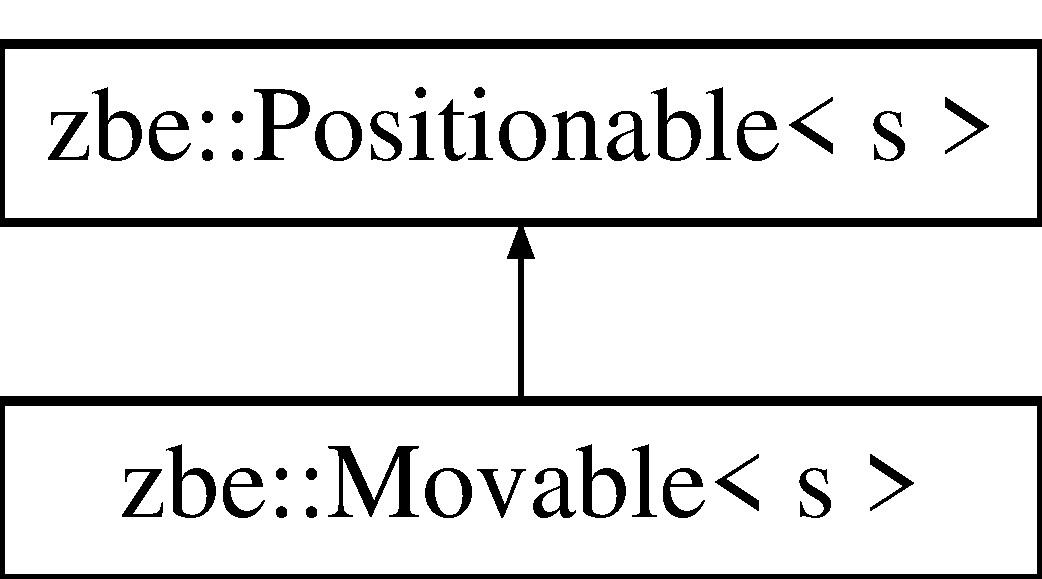
\includegraphics[height=2.000000cm]{classzbe_1_1_movable}
\end{center}
\end{figure}
\subsection*{Public Member Functions}
\begin{DoxyCompactItemize}
\item 
\hyperlink{classzbe_1_1_movable_a391fb1a17f6ff316f9eecdc227e4e7eb}{Movable} ()
\item 
\hyperlink{classzbe_1_1_movable_a38f9dba0d0c33b602f01ac04384afaa7}{Movable} (\hyperlink{classzbe_1_1_point}{Point}$<$ s $>$ position, \hyperlink{classzbe_1_1_vector}{Vector}$<$ s $>$ velocity)
\item 
\hyperlink{classzbe_1_1_movable_a025828ff1b377cf7c4ab463ef8e598ec}{$\sim$\+Movable} ()
\item 
void \hyperlink{classzbe_1_1_movable_aae95d27a429d37f03d5e9a99d30f9fd8}{set\+Velocity} (\hyperlink{classzbe_1_1_vector}{Vector}$<$ s $>$ velocity)
\item 
\hyperlink{classzbe_1_1_vector}{Vector}$<$ s $>$ \hyperlink{classzbe_1_1_movable_a197edd5f791cba551b8465df6bf6e8fb}{get\+Velocity} () const 
\item 
void \hyperlink{classzbe_1_1_movable_a55b00e940046a32fcc24f2fa8847db67}{travel} (double time)
\end{DoxyCompactItemize}


\subsection{Detailed Description}
\subsubsection*{template$<$unsigned s$>$class zbe\+::\+Movable$<$ s $>$}



Definition at line 19 of file Movable.\+h.



\subsection{Constructor \& Destructor Documentation}
\hypertarget{classzbe_1_1_movable_a391fb1a17f6ff316f9eecdc227e4e7eb}{}\index{zbe\+::\+Movable@{zbe\+::\+Movable}!Movable@{Movable}}
\index{Movable@{Movable}!zbe\+::\+Movable@{zbe\+::\+Movable}}
\subsubsection[{Movable()}]{\setlength{\rightskip}{0pt plus 5cm}template$<$unsigned s$>$ {\bf zbe\+::\+Movable}$<$ s $>$\+::{\bf Movable} (
\begin{DoxyParamCaption}
{}
\end{DoxyParamCaption}
)\hspace{0.3cm}{\ttfamily [inline]}}\label{classzbe_1_1_movable_a391fb1a17f6ff316f9eecdc227e4e7eb}


Definition at line 21 of file Movable.\+h.

\hypertarget{classzbe_1_1_movable_a38f9dba0d0c33b602f01ac04384afaa7}{}\index{zbe\+::\+Movable@{zbe\+::\+Movable}!Movable@{Movable}}
\index{Movable@{Movable}!zbe\+::\+Movable@{zbe\+::\+Movable}}
\subsubsection[{Movable(\+Point$<$ s $>$ position, Vector$<$ s $>$ velocity)}]{\setlength{\rightskip}{0pt plus 5cm}template$<$unsigned s$>$ {\bf zbe\+::\+Movable}$<$ s $>$\+::{\bf Movable} (
\begin{DoxyParamCaption}
\item[{{\bf Point}$<$ s $>$}]{position, }
\item[{{\bf Vector}$<$ s $>$}]{velocity}
\end{DoxyParamCaption}
)\hspace{0.3cm}{\ttfamily [inline]}}\label{classzbe_1_1_movable_a38f9dba0d0c33b602f01ac04384afaa7}


Definition at line 23 of file Movable.\+h.

\hypertarget{classzbe_1_1_movable_a025828ff1b377cf7c4ab463ef8e598ec}{}\index{zbe\+::\+Movable@{zbe\+::\+Movable}!````~Movable@{$\sim$\+Movable}}
\index{````~Movable@{$\sim$\+Movable}!zbe\+::\+Movable@{zbe\+::\+Movable}}
\subsubsection[{$\sim$\+Movable()}]{\setlength{\rightskip}{0pt plus 5cm}template$<$unsigned s$>$ {\bf zbe\+::\+Movable}$<$ s $>$\+::$\sim${\bf Movable} (
\begin{DoxyParamCaption}
{}
\end{DoxyParamCaption}
)\hspace{0.3cm}{\ttfamily [inline]}}\label{classzbe_1_1_movable_a025828ff1b377cf7c4ab463ef8e598ec}


Definition at line 25 of file Movable.\+h.



\subsection{Member Function Documentation}
\hypertarget{classzbe_1_1_movable_a197edd5f791cba551b8465df6bf6e8fb}{}\index{zbe\+::\+Movable@{zbe\+::\+Movable}!get\+Velocity@{get\+Velocity}}
\index{get\+Velocity@{get\+Velocity}!zbe\+::\+Movable@{zbe\+::\+Movable}}
\subsubsection[{get\+Velocity() const }]{\setlength{\rightskip}{0pt plus 5cm}template$<$unsigned s$>$ {\bf Vector}$<$s$>$ {\bf zbe\+::\+Movable}$<$ s $>$\+::get\+Velocity (
\begin{DoxyParamCaption}
{}
\end{DoxyParamCaption}
) const\hspace{0.3cm}{\ttfamily [inline]}}\label{classzbe_1_1_movable_a197edd5f791cba551b8465df6bf6e8fb}


Definition at line 28 of file Movable.\+h.

\hypertarget{classzbe_1_1_movable_aae95d27a429d37f03d5e9a99d30f9fd8}{}\index{zbe\+::\+Movable@{zbe\+::\+Movable}!set\+Velocity@{set\+Velocity}}
\index{set\+Velocity@{set\+Velocity}!zbe\+::\+Movable@{zbe\+::\+Movable}}
\subsubsection[{set\+Velocity(\+Vector$<$ s $>$ velocity)}]{\setlength{\rightskip}{0pt plus 5cm}template$<$unsigned s$>$ void {\bf zbe\+::\+Movable}$<$ s $>$\+::set\+Velocity (
\begin{DoxyParamCaption}
\item[{{\bf Vector}$<$ s $>$}]{velocity}
\end{DoxyParamCaption}
)\hspace{0.3cm}{\ttfamily [inline]}}\label{classzbe_1_1_movable_aae95d27a429d37f03d5e9a99d30f9fd8}


Definition at line 27 of file Movable.\+h.

\hypertarget{classzbe_1_1_movable_a55b00e940046a32fcc24f2fa8847db67}{}\index{zbe\+::\+Movable@{zbe\+::\+Movable}!travel@{travel}}
\index{travel@{travel}!zbe\+::\+Movable@{zbe\+::\+Movable}}
\subsubsection[{travel(double time)}]{\setlength{\rightskip}{0pt plus 5cm}template$<$unsigned s$>$ void {\bf zbe\+::\+Movable}$<$ s $>$\+::travel (
\begin{DoxyParamCaption}
\item[{double}]{time}
\end{DoxyParamCaption}
)\hspace{0.3cm}{\ttfamily [inline]}}\label{classzbe_1_1_movable_a55b00e940046a32fcc24f2fa8847db67}


Definition at line 30 of file Movable.\+h.



The documentation for this class was generated from the following file\+:\begin{DoxyCompactItemize}
\item 
include/\+Z\+B\+E/core/archetypes/\hyperlink{_movable_8h}{Movable.\+h}\end{DoxyCompactItemize}

\hypertarget{structzbe_1_1_n_sphere}{}\section{zbe\+:\+:N\+Sphere$<$ s $>$ Struct Template Reference}
\label{structzbe_1_1_n_sphere}\index{zbe\+::\+N\+Sphere$<$ s $>$@{zbe\+::\+N\+Sphere$<$ s $>$}}


{\ttfamily \#include $<$objects.\+h$>$}

\subsection*{Public Member Functions}
\begin{DoxyCompactItemize}
\item 
\hyperlink{structzbe_1_1_n_sphere_a51470e4b5458d4fca454de310cff1bd6}{N\+Sphere} ()
\item 
\hyperlink{structzbe_1_1_n_sphere_af4863ac7a99086b089328b590fb65eb6}{N\+Sphere} (\hyperlink{classzbe_1_1_point}{Point}$<$ s $>$ center, double radius)
\item 
\hyperlink{structzbe_1_1_n_sphere_afcecbe0890ba0e723bbd092e0e598f80}{N\+Sphere} (std\+::initializer\+\_\+list$<$ double $>$ lc, double \hyperlink{structzbe_1_1_n_sphere_ac8fae694bd80717eec61699b4d5206c6}{r})
\end{DoxyCompactItemize}
\subsection*{Public Attributes}
\begin{DoxyCompactItemize}
\item 
\hyperlink{classzbe_1_1_point}{Point}$<$ s $>$ \hyperlink{structzbe_1_1_n_sphere_a4e3c36d361b729674a9e62e37824339e}{c}
\item 
double \hyperlink{structzbe_1_1_n_sphere_ac8fae694bd80717eec61699b4d5206c6}{r}
\end{DoxyCompactItemize}


\subsection{Detailed Description}
\subsubsection*{template$<$unsigned s$>$struct zbe\+::\+N\+Sphere$<$ s $>$}



Definition at line 44 of file objects.\+h.



\subsection{Constructor \& Destructor Documentation}
\hypertarget{structzbe_1_1_n_sphere_a51470e4b5458d4fca454de310cff1bd6}{}\index{zbe\+::\+N\+Sphere@{zbe\+::\+N\+Sphere}!N\+Sphere@{N\+Sphere}}
\index{N\+Sphere@{N\+Sphere}!zbe\+::\+N\+Sphere@{zbe\+::\+N\+Sphere}}
\subsubsection[{N\+Sphere()}]{\setlength{\rightskip}{0pt plus 5cm}template$<$unsigned s$>$ {\bf zbe\+::\+N\+Sphere}$<$ s $>$\+::{\bf N\+Sphere} (
\begin{DoxyParamCaption}
{}
\end{DoxyParamCaption}
)\hspace{0.3cm}{\ttfamily [inline]}}\label{structzbe_1_1_n_sphere_a51470e4b5458d4fca454de310cff1bd6}


Definition at line 45 of file objects.\+h.

\hypertarget{structzbe_1_1_n_sphere_af4863ac7a99086b089328b590fb65eb6}{}\index{zbe\+::\+N\+Sphere@{zbe\+::\+N\+Sphere}!N\+Sphere@{N\+Sphere}}
\index{N\+Sphere@{N\+Sphere}!zbe\+::\+N\+Sphere@{zbe\+::\+N\+Sphere}}
\subsubsection[{N\+Sphere(\+Point$<$ s $>$ center, double radius)}]{\setlength{\rightskip}{0pt plus 5cm}template$<$unsigned s$>$ {\bf zbe\+::\+N\+Sphere}$<$ s $>$\+::{\bf N\+Sphere} (
\begin{DoxyParamCaption}
\item[{{\bf Point}$<$ s $>$}]{center, }
\item[{double}]{radius}
\end{DoxyParamCaption}
)\hspace{0.3cm}{\ttfamily [inline]}}\label{structzbe_1_1_n_sphere_af4863ac7a99086b089328b590fb65eb6}


Definition at line 46 of file objects.\+h.

\hypertarget{structzbe_1_1_n_sphere_afcecbe0890ba0e723bbd092e0e598f80}{}\index{zbe\+::\+N\+Sphere@{zbe\+::\+N\+Sphere}!N\+Sphere@{N\+Sphere}}
\index{N\+Sphere@{N\+Sphere}!zbe\+::\+N\+Sphere@{zbe\+::\+N\+Sphere}}
\subsubsection[{N\+Sphere(std\+::initializer\+\_\+list$<$ double $>$ lc, double r)}]{\setlength{\rightskip}{0pt plus 5cm}template$<$unsigned s$>$ {\bf zbe\+::\+N\+Sphere}$<$ s $>$\+::{\bf N\+Sphere} (
\begin{DoxyParamCaption}
\item[{std\+::initializer\+\_\+list$<$ double $>$}]{lc, }
\item[{double}]{r}
\end{DoxyParamCaption}
)\hspace{0.3cm}{\ttfamily [inline]}}\label{structzbe_1_1_n_sphere_afcecbe0890ba0e723bbd092e0e598f80}


Definition at line 47 of file objects.\+h.



\subsection{Member Data Documentation}
\hypertarget{structzbe_1_1_n_sphere_a4e3c36d361b729674a9e62e37824339e}{}\index{zbe\+::\+N\+Sphere@{zbe\+::\+N\+Sphere}!c@{c}}
\index{c@{c}!zbe\+::\+N\+Sphere@{zbe\+::\+N\+Sphere}}
\subsubsection[{c}]{\setlength{\rightskip}{0pt plus 5cm}template$<$unsigned s$>$ {\bf Point}$<$s$>$ {\bf zbe\+::\+N\+Sphere}$<$ s $>$\+::c}\label{structzbe_1_1_n_sphere_a4e3c36d361b729674a9e62e37824339e}


Definition at line 49 of file objects.\+h.

\hypertarget{structzbe_1_1_n_sphere_ac8fae694bd80717eec61699b4d5206c6}{}\index{zbe\+::\+N\+Sphere@{zbe\+::\+N\+Sphere}!r@{r}}
\index{r@{r}!zbe\+::\+N\+Sphere@{zbe\+::\+N\+Sphere}}
\subsubsection[{r}]{\setlength{\rightskip}{0pt plus 5cm}template$<$unsigned s$>$ double {\bf zbe\+::\+N\+Sphere}$<$ s $>$\+::r}\label{structzbe_1_1_n_sphere_ac8fae694bd80717eec61699b4d5206c6}


Definition at line 50 of file objects.\+h.



The documentation for this struct was generated from the following file\+:\begin{DoxyCompactItemize}
\item 
include/\+Z\+B\+E/core/tools/math/\hyperlink{objects_8h}{objects.\+h}\end{DoxyCompactItemize}

\hypertarget{classzbe_1_1_point}{}\section{zbe\+:\+:Point$<$ s $>$ Class Template Reference}
\label{classzbe_1_1_point}\index{zbe\+::\+Point$<$ s $>$@{zbe\+::\+Point$<$ s $>$}}


A class that represent Points of any dimension.  




{\ttfamily \#include $<$Point.\+h$>$}

\subsection*{Public Member Functions}
\begin{DoxyCompactItemize}
\item 
\hyperlink{classzbe_1_1_point_a2f4b573c8afece71382e36e8a972c768}{Point} ()
\begin{DoxyCompactList}\small\item\em Void constructor, the \hyperlink{classzbe_1_1_point}{Point}\textquotesingle{}s values are unknown. \end{DoxyCompactList}\item 
\hyperlink{classzbe_1_1_point_aebca7e4128f8cc20a0d2862126619aab}{Point} (const std\+::initializer\+\_\+list$<$ double $>$ l)
\begin{DoxyCompactList}\small\item\em A list initializer constructor. \end{DoxyCompactList}\item 
double \& \hyperlink{classzbe_1_1_point_a3f60b81f07951c6e1a012cfdd903c27a}{operator\mbox{[}$\,$\mbox{]}} (std\+::size\+\_\+t idx)
\begin{DoxyCompactList}\small\item\em Implements direct access to \hyperlink{classzbe_1_1_point}{Point} values with operator\mbox{[}\mbox{]}. \end{DoxyCompactList}\item 
const double \& \hyperlink{classzbe_1_1_point_a4a928fbbd33b681f7e7a1a0ab7f3ac92}{operator\mbox{[}$\,$\mbox{]}} (std\+::size\+\_\+t idx) const 
\begin{DoxyCompactList}\small\item\em Implements direct access to \hyperlink{classzbe_1_1_point}{Point} values with operator\mbox{[}\mbox{]}. \end{DoxyCompactList}\item 
\hyperlink{classzbe_1_1_point}{Point} \& \hyperlink{classzbe_1_1_point_affd866729abeadf7cfed39e9cc7148c4}{operator+=} (\hyperlink{classzbe_1_1_vector}{Vector}$<$ s $>$ rhs)
\begin{DoxyCompactList}\small\item\em Translate a \hyperlink{classzbe_1_1_point}{Point} in the direction of a \hyperlink{classzbe_1_1_vector}{Vector}. \end{DoxyCompactList}\item 
\hyperlink{classzbe_1_1_point}{Point} \& \hyperlink{classzbe_1_1_point_a7a0c2c5f931f27051bdb4e0ef8e25633}{operator$\ast$=} (double rhs)
\begin{DoxyCompactList}\small\item\em Multiply a \hyperlink{classzbe_1_1_point}{Point} by a scalar. \end{DoxyCompactList}\end{DoxyCompactItemize}
\subsection*{Protected Attributes}
\begin{DoxyCompactItemize}
\item 
double \hyperlink{classzbe_1_1_point_a44784a8fc0112f976473e8e2da0193e5}{data} \mbox{[}s\mbox{]}
\begin{DoxyCompactList}\small\item\em \hyperlink{classzbe_1_1_point}{Point} data. \end{DoxyCompactList}\end{DoxyCompactItemize}
\subsection*{Friends}
\begin{DoxyCompactItemize}
\item 
\hyperlink{classzbe_1_1_point}{Point} \hyperlink{classzbe_1_1_point_a74ace46c2a8478251d76bceef6715c6d}{operator+} (\hyperlink{classzbe_1_1_point}{Point} lhs, const \hyperlink{classzbe_1_1_vector}{Vector}$<$ s $>$ \&rhs)
\begin{DoxyCompactList}\small\item\em Translate a \hyperlink{classzbe_1_1_point}{Point} in the direction of a \hyperlink{classzbe_1_1_vector}{Vector}. \end{DoxyCompactList}\item 
\hyperlink{classzbe_1_1_vector}{Vector}$<$ s $>$ \hyperlink{classzbe_1_1_point_afd14d87b02bf3ff8a034483748ba0f44}{operator-\/} (const \hyperlink{classzbe_1_1_point}{Point} \&lhs, const \hyperlink{classzbe_1_1_point}{Point} \&rhs)
\begin{DoxyCompactList}\small\item\em Calculate the \hyperlink{classzbe_1_1_vector}{Vector} that connects two Points. \end{DoxyCompactList}\item 
\hyperlink{classzbe_1_1_point}{Point} \hyperlink{classzbe_1_1_point_a5a5836772aa1d8dd4666c553c9b1ce45}{operator$\ast$} (\hyperlink{classzbe_1_1_point}{Point} lhs, double rhs)
\begin{DoxyCompactList}\small\item\em Multiply a \hyperlink{classzbe_1_1_point}{Point} by a scalar. \end{DoxyCompactList}\end{DoxyCompactItemize}


\subsection{Detailed Description}
\subsubsection*{template$<$unsigned s$>$class zbe\+::\+Point$<$ s $>$}

A class that represent Points of any dimension. 

This template needs to know the number of dimensions of the hyperplane to which the \hyperlink{classzbe_1_1_point}{Point} belongs. 

Definition at line 27 of file Point.\+h.



\subsection{Constructor \& Destructor Documentation}
\hypertarget{classzbe_1_1_point_a2f4b573c8afece71382e36e8a972c768}{}\index{zbe\+::\+Point@{zbe\+::\+Point}!Point@{Point}}
\index{Point@{Point}!zbe\+::\+Point@{zbe\+::\+Point}}
\subsubsection[{Point()}]{\setlength{\rightskip}{0pt plus 5cm}template$<$unsigned s$>$ {\bf zbe\+::\+Point}$<$ s $>$\+::{\bf Point} (
\begin{DoxyParamCaption}
{}
\end{DoxyParamCaption}
)\hspace{0.3cm}{\ttfamily [inline]}}\label{classzbe_1_1_point_a2f4b573c8afece71382e36e8a972c768}


Void constructor, the \hyperlink{classzbe_1_1_point}{Point}\textquotesingle{}s values are unknown. 



Definition at line 32 of file Point.\+h.

\hypertarget{classzbe_1_1_point_aebca7e4128f8cc20a0d2862126619aab}{}\index{zbe\+::\+Point@{zbe\+::\+Point}!Point@{Point}}
\index{Point@{Point}!zbe\+::\+Point@{zbe\+::\+Point}}
\subsubsection[{Point(const std\+::initializer\+\_\+list$<$ double $>$ l)}]{\setlength{\rightskip}{0pt plus 5cm}template$<$unsigned s$>$ {\bf zbe\+::\+Point}$<$ s $>$\+::{\bf Point} (
\begin{DoxyParamCaption}
\item[{const std\+::initializer\+\_\+list$<$ double $>$}]{l}
\end{DoxyParamCaption}
)\hspace{0.3cm}{\ttfamily [inline]}}\label{classzbe_1_1_point_aebca7e4128f8cc20a0d2862126619aab}


A list initializer constructor. 

You can create a \hyperlink{classzbe_1_1_point}{Point} of N dimension with a list of N values\+: \begin{DoxyVerb}  Point<N> p(v1, v2, ... , vN)
\end{DoxyVerb}


or \begin{DoxyVerb}  Point<N> p = {v1, v2, ... , vN}\end{DoxyVerb}
 

Definition at line 45 of file Point.\+h.



\subsection{Member Function Documentation}
\hypertarget{classzbe_1_1_point_a7a0c2c5f931f27051bdb4e0ef8e25633}{}\index{zbe\+::\+Point@{zbe\+::\+Point}!operator$\ast$=@{operator$\ast$=}}
\index{operator$\ast$=@{operator$\ast$=}!zbe\+::\+Point@{zbe\+::\+Point}}
\subsubsection[{operator$\ast$=(double rhs)}]{\setlength{\rightskip}{0pt plus 5cm}template$<$unsigned s$>$ {\bf Point}\& {\bf zbe\+::\+Point}$<$ s $>$\+::operator$\ast$= (
\begin{DoxyParamCaption}
\item[{double}]{rhs}
\end{DoxyParamCaption}
)\hspace{0.3cm}{\ttfamily [inline]}}\label{classzbe_1_1_point_a7a0c2c5f931f27051bdb4e0ef8e25633}


Multiply a \hyperlink{classzbe_1_1_point}{Point} by a scalar. 

The resulting \hyperlink{classzbe_1_1_point}{Point} is as follows\+: \begin{DoxyVerb}  Point<2> p(1,2);
  p *= 3;
\end{DoxyVerb}


p values are (3,6).


\begin{DoxyParams}{Parameters}
{\em rhs} & The scalar. \\
\hline
\end{DoxyParams}
\begin{DoxyReturn}{Returns}
A reference to this \hyperlink{classzbe_1_1_point}{Point}. 
\end{DoxyReturn}
\begin{DoxySeeAlso}{See also}
\hyperlink{classzbe_1_1_point_affd866729abeadf7cfed39e9cc7148c4}{operator+=()} 
\end{DoxySeeAlso}


Definition at line 104 of file Point.\+h.

\hypertarget{classzbe_1_1_point_affd866729abeadf7cfed39e9cc7148c4}{}\index{zbe\+::\+Point@{zbe\+::\+Point}!operator+=@{operator+=}}
\index{operator+=@{operator+=}!zbe\+::\+Point@{zbe\+::\+Point}}
\subsubsection[{operator+=(\+Vector$<$ s $>$ rhs)}]{\setlength{\rightskip}{0pt plus 5cm}template$<$unsigned s$>$ {\bf Point}\& {\bf zbe\+::\+Point}$<$ s $>$\+::operator+= (
\begin{DoxyParamCaption}
\item[{{\bf Vector}$<$ s $>$}]{rhs}
\end{DoxyParamCaption}
)\hspace{0.3cm}{\ttfamily [inline]}}\label{classzbe_1_1_point_affd866729abeadf7cfed39e9cc7148c4}


Translate a \hyperlink{classzbe_1_1_point}{Point} in the direction of a \hyperlink{classzbe_1_1_vector}{Vector}. 


\begin{DoxyParams}{Parameters}
{\em rhs} & \hyperlink{classzbe_1_1_vector}{Vector} in which you want to move the \hyperlink{classzbe_1_1_point}{Point}. \\
\hline
\end{DoxyParams}
\begin{DoxyReturn}{Returns}
A reference to this \hyperlink{classzbe_1_1_point}{Point}. 
\end{DoxyReturn}
\begin{DoxySeeAlso}{See also}
\hyperlink{classzbe_1_1_point_a7a0c2c5f931f27051bdb4e0ef8e25633}{operator$\ast$=()} 
\end{DoxySeeAlso}


Definition at line 83 of file Point.\+h.

\hypertarget{classzbe_1_1_point_a3f60b81f07951c6e1a012cfdd903c27a}{}\index{zbe\+::\+Point@{zbe\+::\+Point}!operator\mbox{[}$\,$\mbox{]}@{operator[]}}
\index{operator\mbox{[}$\,$\mbox{]}@{operator[]}!zbe\+::\+Point@{zbe\+::\+Point}}
\subsubsection[{operator[](std\+::size\+\_\+t idx)}]{\setlength{\rightskip}{0pt plus 5cm}template$<$unsigned s$>$ double\& {\bf zbe\+::\+Point}$<$ s $>$\+::operator\mbox{[}$\,$\mbox{]} (
\begin{DoxyParamCaption}
\item[{std\+::size\+\_\+t}]{idx}
\end{DoxyParamCaption}
)\hspace{0.3cm}{\ttfamily [inline]}}\label{classzbe_1_1_point_a3f60b81f07951c6e1a012cfdd903c27a}


Implements direct access to \hyperlink{classzbe_1_1_point}{Point} values with operator\mbox{[}\mbox{]}. 

No bound checking is performed, the behavior accessing an out of bound index is undefined.


\begin{DoxyParams}{Parameters}
{\em idx} & Index of the dimension that you want to get the value. \\
\hline
\end{DoxyParams}
\begin{DoxyReturn}{Returns}
The value of the idx dimension. 
\end{DoxyReturn}


Definition at line 65 of file Point.\+h.

\hypertarget{classzbe_1_1_point_a4a928fbbd33b681f7e7a1a0ab7f3ac92}{}\index{zbe\+::\+Point@{zbe\+::\+Point}!operator\mbox{[}$\,$\mbox{]}@{operator[]}}
\index{operator\mbox{[}$\,$\mbox{]}@{operator[]}!zbe\+::\+Point@{zbe\+::\+Point}}
\subsubsection[{operator[](std\+::size\+\_\+t idx) const }]{\setlength{\rightskip}{0pt plus 5cm}template$<$unsigned s$>$ const double\& {\bf zbe\+::\+Point}$<$ s $>$\+::operator\mbox{[}$\,$\mbox{]} (
\begin{DoxyParamCaption}
\item[{std\+::size\+\_\+t}]{idx}
\end{DoxyParamCaption}
) const\hspace{0.3cm}{\ttfamily [inline]}}\label{classzbe_1_1_point_a4a928fbbd33b681f7e7a1a0ab7f3ac92}


Implements direct access to \hyperlink{classzbe_1_1_point}{Point} values with operator\mbox{[}\mbox{]}. 

No bound checking is performed, the behavior accessing an out of bound index is undefined.


\begin{DoxyParams}{Parameters}
{\em idx} & Index of the dimension that you want to get the value. \\
\hline
\end{DoxyParams}
\begin{DoxyReturn}{Returns}
The constant value of the idx dimension. 
\end{DoxyReturn}


Definition at line 75 of file Point.\+h.



\subsection{Friends And Related Function Documentation}
\hypertarget{classzbe_1_1_point_a5a5836772aa1d8dd4666c553c9b1ce45}{}\index{zbe\+::\+Point@{zbe\+::\+Point}!operator$\ast$@{operator$\ast$}}
\index{operator$\ast$@{operator$\ast$}!zbe\+::\+Point@{zbe\+::\+Point}}
\subsubsection[{operator$\ast$}]{\setlength{\rightskip}{0pt plus 5cm}template$<$unsigned s$>$ {\bf Point} operator$\ast$ (
\begin{DoxyParamCaption}
\item[{{\bf Point}$<$ s $>$}]{lhs, }
\item[{double}]{rhs}
\end{DoxyParamCaption}
)\hspace{0.3cm}{\ttfamily [friend]}}\label{classzbe_1_1_point_a5a5836772aa1d8dd4666c553c9b1ce45}


Multiply a \hyperlink{classzbe_1_1_point}{Point} by a scalar. 

The resulting \hyperlink{classzbe_1_1_point}{Point} is as follows\+: \begin{DoxyVerb}  Point<2> p(1,2);
  Point<2> q = p * 3;
\end{DoxyVerb}


q values are (3,6).


\begin{DoxyParams}{Parameters}
{\em lhs} & The initial \hyperlink{classzbe_1_1_point}{Point}. \\
\hline
{\em rhs} & The scalar. \\
\hline
\end{DoxyParams}
\begin{DoxyReturn}{Returns}
The resulting \hyperlink{classzbe_1_1_point}{Point} of multiplying the initial point by the scalar. 
\end{DoxyReturn}


Definition at line 152 of file Point.\+h.

\hypertarget{classzbe_1_1_point_a74ace46c2a8478251d76bceef6715c6d}{}\index{zbe\+::\+Point@{zbe\+::\+Point}!operator+@{operator+}}
\index{operator+@{operator+}!zbe\+::\+Point@{zbe\+::\+Point}}
\subsubsection[{operator+}]{\setlength{\rightskip}{0pt plus 5cm}template$<$unsigned s$>$ {\bf Point} operator+ (
\begin{DoxyParamCaption}
\item[{{\bf Point}$<$ s $>$}]{lhs, }
\item[{const {\bf Vector}$<$ s $>$ \&}]{rhs}
\end{DoxyParamCaption}
)\hspace{0.3cm}{\ttfamily [friend]}}\label{classzbe_1_1_point_a74ace46c2a8478251d76bceef6715c6d}


Translate a \hyperlink{classzbe_1_1_point}{Point} in the direction of a \hyperlink{classzbe_1_1_vector}{Vector}. 


\begin{DoxyParams}{Parameters}
{\em lhs} & The initial \hyperlink{classzbe_1_1_point}{Point}. \\
\hline
{\em rhs} & \hyperlink{classzbe_1_1_vector}{Vector} in which you want to move the \hyperlink{classzbe_1_1_point}{Point}. \\
\hline
\end{DoxyParams}
\begin{DoxyReturn}{Returns}
A new \hyperlink{classzbe_1_1_point}{Point} with the result of the translation. 
\end{DoxyReturn}


Definition at line 118 of file Point.\+h.

\hypertarget{classzbe_1_1_point_afd14d87b02bf3ff8a034483748ba0f44}{}\index{zbe\+::\+Point@{zbe\+::\+Point}!operator-\/@{operator-\/}}
\index{operator-\/@{operator-\/}!zbe\+::\+Point@{zbe\+::\+Point}}
\subsubsection[{operator-\/}]{\setlength{\rightskip}{0pt plus 5cm}template$<$unsigned s$>$ {\bf Vector}$<$s$>$ operator-\/ (
\begin{DoxyParamCaption}
\item[{const {\bf Point}$<$ s $>$ \&}]{lhs, }
\item[{const {\bf Point}$<$ s $>$ \&}]{rhs}
\end{DoxyParamCaption}
)\hspace{0.3cm}{\ttfamily [friend]}}\label{classzbe_1_1_point_afd14d87b02bf3ff8a034483748ba0f44}


Calculate the \hyperlink{classzbe_1_1_vector}{Vector} that connects two Points. 


\begin{DoxyParams}{Parameters}
{\em lhs} & The initial \hyperlink{classzbe_1_1_point}{Point}. \\
\hline
{\em rhs} & The destiny \hyperlink{classzbe_1_1_point}{Point}. \\
\hline
\end{DoxyParams}
\begin{DoxyReturn}{Returns}
A \hyperlink{classzbe_1_1_vector}{Vector} that translate the initial \hyperlink{classzbe_1_1_point}{Point} to the destination \hyperlink{classzbe_1_1_point}{Point}. 
\end{DoxyReturn}


Definition at line 129 of file Point.\+h.



\subsection{Member Data Documentation}
\hypertarget{classzbe_1_1_point_a44784a8fc0112f976473e8e2da0193e5}{}\index{zbe\+::\+Point@{zbe\+::\+Point}!data@{data}}
\index{data@{data}!zbe\+::\+Point@{zbe\+::\+Point}}
\subsubsection[{data}]{\setlength{\rightskip}{0pt plus 5cm}template$<$unsigned s$>$ double {\bf zbe\+::\+Point}$<$ s $>$\+::data\mbox{[}s\mbox{]}\hspace{0.3cm}{\ttfamily [protected]}}\label{classzbe_1_1_point_a44784a8fc0112f976473e8e2da0193e5}


\hyperlink{classzbe_1_1_point}{Point} data. 



Definition at line 161 of file Point.\+h.



The documentation for this class was generated from the following file\+:\begin{DoxyCompactItemize}
\item 
include/\+Z\+B\+E/core/tools/math/\hyperlink{_point_8h}{Point.\+h}\end{DoxyCompactItemize}

\hypertarget{classzbe_1_1_point2_d}{}\section{zbe\+:\+:Point2\+D Class Reference}
\label{classzbe_1_1_point2_d}\index{zbe\+::\+Point2\+D@{zbe\+::\+Point2\+D}}


An aliases of a \hyperlink{classzbe_1_1_point}{Point$<$2$>$}.  




{\ttfamily \#include $<$Point.\+h$>$}

Inheritance diagram for zbe\+:\+:Point2\+D\+:\begin{figure}[H]
\begin{center}
\leavevmode
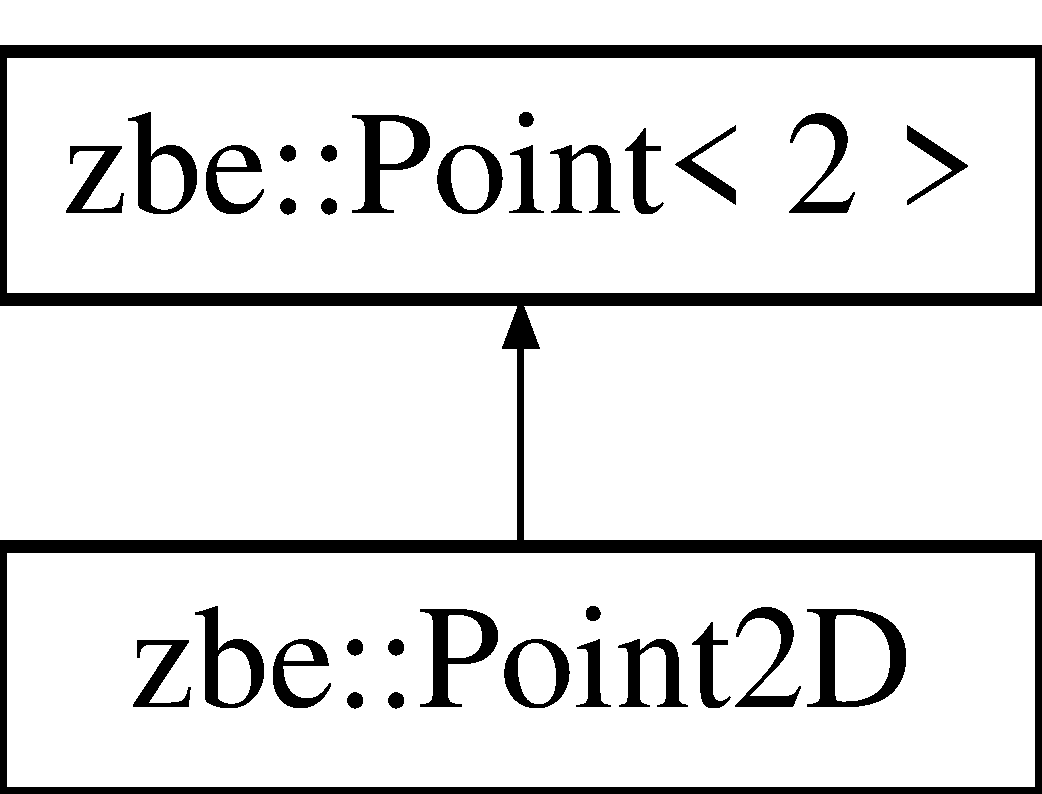
\includegraphics[height=2.000000cm]{classzbe_1_1_point2_d}
\end{center}
\end{figure}
\subsection*{Public Member Functions}
\begin{DoxyCompactItemize}
\item 
\hyperlink{classzbe_1_1_point2_d_a377ba7e87a56d280fb66c666ccfc873e}{Point2\+D} ()
\begin{DoxyCompactList}\small\item\em Void constructor, the \hyperlink{classzbe_1_1_point2_d}{Point2\+D}\textquotesingle{}s values are unknown. \end{DoxyCompactList}\item 
\hyperlink{classzbe_1_1_point2_d_a6a385429fc369e6d56a73497b4a3ea67}{Point2\+D} (const \hyperlink{classzbe_1_1_point}{Point}$<$ 2 $>$ \&p)
\begin{DoxyCompactList}\small\item\em A copy constructor with \hyperlink{classzbe_1_1_point}{Point$<$2$>$}. \end{DoxyCompactList}\item 
\hyperlink{classzbe_1_1_point2_d_adb2dfc5d538078d361d21a418553b4d0}{Point2\+D} (std\+::initializer\+\_\+list$<$ double $>$ l)
\begin{DoxyCompactList}\small\item\em A list initializer constructor. \end{DoxyCompactList}\item 
\hyperlink{classzbe_1_1_point2_d}{Point2\+D} \& \hyperlink{classzbe_1_1_point2_d_a01ef2d238d9c648676eacc4946bd12b7}{operator=} (\hyperlink{classzbe_1_1_point}{Point}$<$ 2 $>$ rhs)
\begin{DoxyCompactList}\small\item\em This class let you compare \hyperlink{classzbe_1_1_point}{Point$<$2$>$} with \hyperlink{classzbe_1_1_point2_d}{Point2\+D} classes. \end{DoxyCompactList}\end{DoxyCompactItemize}
\subsection*{Public Attributes}
\begin{DoxyCompactItemize}
\item 
double \& \hyperlink{classzbe_1_1_point2_d_a72346e41165fedab5dfddda9164f07fc}{x} = \hyperlink{classzbe_1_1_point_a44784a8fc0112f976473e8e2da0193e5}{data}\mbox{[}0\mbox{]}
\begin{DoxyCompactList}\small\item\em An alias to access the first dimension as p.\+x. \end{DoxyCompactList}\item 
double \& \hyperlink{classzbe_1_1_point2_d_a9f1e20366f38743e2d3264bd4cb633f2}{y} = \hyperlink{classzbe_1_1_point_a44784a8fc0112f976473e8e2da0193e5}{data}\mbox{[}1\mbox{]}
\begin{DoxyCompactList}\small\item\em An alias to access the second dimension as p.\+y. \end{DoxyCompactList}\end{DoxyCompactItemize}
\subsection*{Additional Inherited Members}


\subsection{Detailed Description}
An aliases of a \hyperlink{classzbe_1_1_point}{Point$<$2$>$}. 

Used to implement some functionality of a 2 dimensional \hyperlink{classzbe_1_1_point}{Point}. 

Definition at line 168 of file Point.\+h.



\subsection{Constructor \& Destructor Documentation}
\hypertarget{classzbe_1_1_point2_d_a377ba7e87a56d280fb66c666ccfc873e}{}\index{zbe\+::\+Point2\+D@{zbe\+::\+Point2\+D}!Point2\+D@{Point2\+D}}
\index{Point2\+D@{Point2\+D}!zbe\+::\+Point2\+D@{zbe\+::\+Point2\+D}}
\subsubsection[{Point2\+D()}]{\setlength{\rightskip}{0pt plus 5cm}zbe\+::\+Point2\+D\+::\+Point2\+D (
\begin{DoxyParamCaption}
{}
\end{DoxyParamCaption}
)\hspace{0.3cm}{\ttfamily [inline]}}\label{classzbe_1_1_point2_d_a377ba7e87a56d280fb66c666ccfc873e}


Void constructor, the \hyperlink{classzbe_1_1_point2_d}{Point2\+D}\textquotesingle{}s values are unknown. 



Definition at line 175 of file Point.\+h.

\hypertarget{classzbe_1_1_point2_d_a6a385429fc369e6d56a73497b4a3ea67}{}\index{zbe\+::\+Point2\+D@{zbe\+::\+Point2\+D}!Point2\+D@{Point2\+D}}
\index{Point2\+D@{Point2\+D}!zbe\+::\+Point2\+D@{zbe\+::\+Point2\+D}}
\subsubsection[{Point2\+D(const Point$<$ 2 $>$ \&p)}]{\setlength{\rightskip}{0pt plus 5cm}zbe\+::\+Point2\+D\+::\+Point2\+D (
\begin{DoxyParamCaption}
\item[{const {\bf Point}$<$ 2 $>$ \&}]{p}
\end{DoxyParamCaption}
)\hspace{0.3cm}{\ttfamily [inline]}}\label{classzbe_1_1_point2_d_a6a385429fc369e6d56a73497b4a3ea67}


A copy constructor with \hyperlink{classzbe_1_1_point}{Point$<$2$>$}. 



Definition at line 179 of file Point.\+h.

\hypertarget{classzbe_1_1_point2_d_adb2dfc5d538078d361d21a418553b4d0}{}\index{zbe\+::\+Point2\+D@{zbe\+::\+Point2\+D}!Point2\+D@{Point2\+D}}
\index{Point2\+D@{Point2\+D}!zbe\+::\+Point2\+D@{zbe\+::\+Point2\+D}}
\subsubsection[{Point2\+D(std\+::initializer\+\_\+list$<$ double $>$ l)}]{\setlength{\rightskip}{0pt plus 5cm}zbe\+::\+Point2\+D\+::\+Point2\+D (
\begin{DoxyParamCaption}
\item[{std\+::initializer\+\_\+list$<$ double $>$}]{l}
\end{DoxyParamCaption}
)\hspace{0.3cm}{\ttfamily [inline]}}\label{classzbe_1_1_point2_d_adb2dfc5d538078d361d21a418553b4d0}


A list initializer constructor. 

You can create a \hyperlink{classzbe_1_1_point2_d}{Point2\+D} with a list of 2 values\+: \begin{DoxyVerb}  Point2D p(v1, v2)
\end{DoxyVerb}


or \begin{DoxyVerb}  Point2D p = {v1, v2}\end{DoxyVerb}
 

Definition at line 192 of file Point.\+h.



\subsection{Member Function Documentation}
\hypertarget{classzbe_1_1_point2_d_a01ef2d238d9c648676eacc4946bd12b7}{}\index{zbe\+::\+Point2\+D@{zbe\+::\+Point2\+D}!operator=@{operator=}}
\index{operator=@{operator=}!zbe\+::\+Point2\+D@{zbe\+::\+Point2\+D}}
\subsubsection[{operator=(\+Point$<$ 2 $>$ rhs)}]{\setlength{\rightskip}{0pt plus 5cm}{\bf Point2\+D}\& zbe\+::\+Point2\+D\+::operator= (
\begin{DoxyParamCaption}
\item[{{\bf Point}$<$ 2 $>$}]{rhs}
\end{DoxyParamCaption}
)\hspace{0.3cm}{\ttfamily [inline]}}\label{classzbe_1_1_point2_d_a01ef2d238d9c648676eacc4946bd12b7}


This class let you compare \hyperlink{classzbe_1_1_point}{Point$<$2$>$} with \hyperlink{classzbe_1_1_point2_d}{Point2\+D} classes. 



Definition at line 196 of file Point.\+h.



\subsection{Member Data Documentation}
\hypertarget{classzbe_1_1_point2_d_a72346e41165fedab5dfddda9164f07fc}{}\index{zbe\+::\+Point2\+D@{zbe\+::\+Point2\+D}!x@{x}}
\index{x@{x}!zbe\+::\+Point2\+D@{zbe\+::\+Point2\+D}}
\subsubsection[{x}]{\setlength{\rightskip}{0pt plus 5cm}double\& zbe\+::\+Point2\+D\+::x = {\bf data}\mbox{[}0\mbox{]}}\label{classzbe_1_1_point2_d_a72346e41165fedab5dfddda9164f07fc}


An alias to access the first dimension as p.\+x. 



Definition at line 170 of file Point.\+h.

\hypertarget{classzbe_1_1_point2_d_a9f1e20366f38743e2d3264bd4cb633f2}{}\index{zbe\+::\+Point2\+D@{zbe\+::\+Point2\+D}!y@{y}}
\index{y@{y}!zbe\+::\+Point2\+D@{zbe\+::\+Point2\+D}}
\subsubsection[{y}]{\setlength{\rightskip}{0pt plus 5cm}double\& zbe\+::\+Point2\+D\+::y = {\bf data}\mbox{[}1\mbox{]}}\label{classzbe_1_1_point2_d_a9f1e20366f38743e2d3264bd4cb633f2}


An alias to access the second dimension as p.\+y. 



Definition at line 171 of file Point.\+h.



The documentation for this class was generated from the following file\+:\begin{DoxyCompactItemize}
\item 
include/\+Z\+B\+E/core/tools/math/\hyperlink{_point_8h}{Point.\+h}\end{DoxyCompactItemize}

\hypertarget{classzbe_1_1_point3_d}{}\section{zbe\+:\+:Point3\+D Class Reference}
\label{classzbe_1_1_point3_d}\index{zbe\+::\+Point3\+D@{zbe\+::\+Point3\+D}}


An aliases of a \hyperlink{classzbe_1_1_point}{Point$<$3$>$}.  




{\ttfamily \#include $<$Point.\+h$>$}

Inheritance diagram for zbe\+:\+:Point3\+D\+:\begin{figure}[H]
\begin{center}
\leavevmode
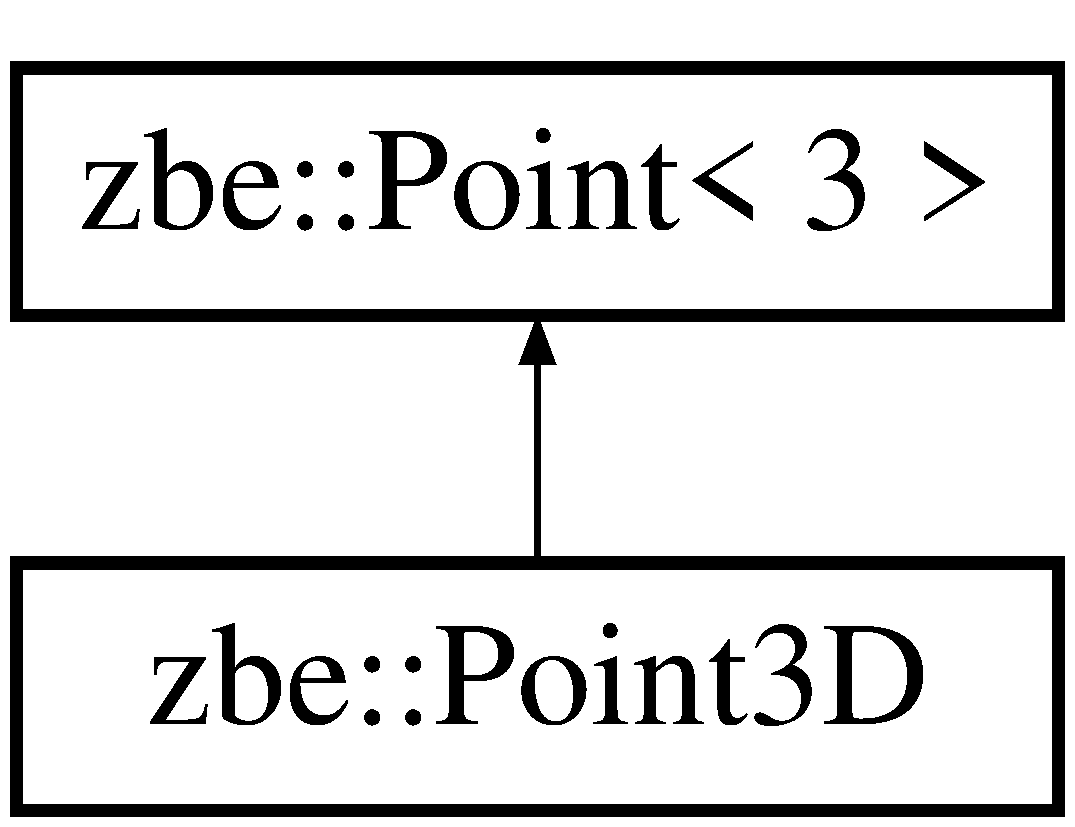
\includegraphics[height=2.000000cm]{classzbe_1_1_point3_d}
\end{center}
\end{figure}
\subsection*{Public Member Functions}
\begin{DoxyCompactItemize}
\item 
\hyperlink{classzbe_1_1_point3_d_ab2ceb379ccb84e342f5dbeeacb6644e5}{Point3\+D} ()
\begin{DoxyCompactList}\small\item\em Void constructor, the \hyperlink{classzbe_1_1_point3_d}{Point3\+D}\textquotesingle{}s values are unknown. \end{DoxyCompactList}\item 
\hyperlink{classzbe_1_1_point3_d_a8d343c388d95bb8baddb912b34d4be62}{Point3\+D} (const \hyperlink{classzbe_1_1_point}{Point}$<$ 3 $>$ \&p)
\begin{DoxyCompactList}\small\item\em A copy constructor with \hyperlink{classzbe_1_1_point}{Point$<$3$>$}. \end{DoxyCompactList}\item 
\hyperlink{classzbe_1_1_point3_d_a389cf92ca16e6bf71df890b29f986609}{Point3\+D} (std\+::initializer\+\_\+list$<$ double $>$ l)
\begin{DoxyCompactList}\small\item\em A list initializer constructor. \end{DoxyCompactList}\item 
\hyperlink{classzbe_1_1_point3_d}{Point3\+D} \& \hyperlink{classzbe_1_1_point3_d_a3deee1b44844d60c3fdabfca0af47379}{operator=} (\hyperlink{classzbe_1_1_point}{Point}$<$ 3 $>$ rhs)
\begin{DoxyCompactList}\small\item\em This class let you compare \hyperlink{classzbe_1_1_point}{Point$<$3$>$} with \hyperlink{classzbe_1_1_point3_d}{Point3\+D} classes. \end{DoxyCompactList}\end{DoxyCompactItemize}
\subsection*{Public Attributes}
\begin{DoxyCompactItemize}
\item 
double \& \hyperlink{classzbe_1_1_point3_d_af5a1cd56dc21df531bc92ab03efa6ee6}{x} = \hyperlink{classzbe_1_1_point_a44784a8fc0112f976473e8e2da0193e5}{data}\mbox{[}0\mbox{]}
\begin{DoxyCompactList}\small\item\em An alias to access the first dimension as p.\+x. \end{DoxyCompactList}\item 
double \& \hyperlink{classzbe_1_1_point3_d_a06bcb3860ed13dfce2d8e95d81fdbea9}{y} = \hyperlink{classzbe_1_1_point_a44784a8fc0112f976473e8e2da0193e5}{data}\mbox{[}1\mbox{]}
\begin{DoxyCompactList}\small\item\em An alias to access the second dimension as p.\+y. \end{DoxyCompactList}\item 
double \& \hyperlink{classzbe_1_1_point3_d_abfa9463b5314e1dbaa2db879ccbb71a4}{z} = \hyperlink{classzbe_1_1_point_a44784a8fc0112f976473e8e2da0193e5}{data}\mbox{[}2\mbox{]}
\begin{DoxyCompactList}\small\item\em An alias to access the third dimension as p.\+z. \end{DoxyCompactList}\end{DoxyCompactItemize}
\subsection*{Additional Inherited Members}


\subsection{Detailed Description}
An aliases of a \hyperlink{classzbe_1_1_point}{Point$<$3$>$}. 

Used to implement some functionality of a 3 dimensional \hyperlink{classzbe_1_1_point}{Point}. 

Definition at line 203 of file Point.\+h.



\subsection{Constructor \& Destructor Documentation}
\hypertarget{classzbe_1_1_point3_d_ab2ceb379ccb84e342f5dbeeacb6644e5}{}\index{zbe\+::\+Point3\+D@{zbe\+::\+Point3\+D}!Point3\+D@{Point3\+D}}
\index{Point3\+D@{Point3\+D}!zbe\+::\+Point3\+D@{zbe\+::\+Point3\+D}}
\subsubsection[{Point3\+D()}]{\setlength{\rightskip}{0pt plus 5cm}zbe\+::\+Point3\+D\+::\+Point3\+D (
\begin{DoxyParamCaption}
{}
\end{DoxyParamCaption}
)\hspace{0.3cm}{\ttfamily [inline]}}\label{classzbe_1_1_point3_d_ab2ceb379ccb84e342f5dbeeacb6644e5}


Void constructor, the \hyperlink{classzbe_1_1_point3_d}{Point3\+D}\textquotesingle{}s values are unknown. 



Definition at line 211 of file Point.\+h.

\hypertarget{classzbe_1_1_point3_d_a8d343c388d95bb8baddb912b34d4be62}{}\index{zbe\+::\+Point3\+D@{zbe\+::\+Point3\+D}!Point3\+D@{Point3\+D}}
\index{Point3\+D@{Point3\+D}!zbe\+::\+Point3\+D@{zbe\+::\+Point3\+D}}
\subsubsection[{Point3\+D(const Point$<$ 3 $>$ \&p)}]{\setlength{\rightskip}{0pt plus 5cm}zbe\+::\+Point3\+D\+::\+Point3\+D (
\begin{DoxyParamCaption}
\item[{const {\bf Point}$<$ 3 $>$ \&}]{p}
\end{DoxyParamCaption}
)\hspace{0.3cm}{\ttfamily [inline]}}\label{classzbe_1_1_point3_d_a8d343c388d95bb8baddb912b34d4be62}


A copy constructor with \hyperlink{classzbe_1_1_point}{Point$<$3$>$}. 



Definition at line 215 of file Point.\+h.

\hypertarget{classzbe_1_1_point3_d_a389cf92ca16e6bf71df890b29f986609}{}\index{zbe\+::\+Point3\+D@{zbe\+::\+Point3\+D}!Point3\+D@{Point3\+D}}
\index{Point3\+D@{Point3\+D}!zbe\+::\+Point3\+D@{zbe\+::\+Point3\+D}}
\subsubsection[{Point3\+D(std\+::initializer\+\_\+list$<$ double $>$ l)}]{\setlength{\rightskip}{0pt plus 5cm}zbe\+::\+Point3\+D\+::\+Point3\+D (
\begin{DoxyParamCaption}
\item[{std\+::initializer\+\_\+list$<$ double $>$}]{l}
\end{DoxyParamCaption}
)\hspace{0.3cm}{\ttfamily [inline]}}\label{classzbe_1_1_point3_d_a389cf92ca16e6bf71df890b29f986609}


A list initializer constructor. 

You can create a \hyperlink{classzbe_1_1_point3_d}{Point3\+D} with a list of 3 values\+: \begin{DoxyVerb}  Point3D p(v1, v2, v3)
\end{DoxyVerb}


or \begin{DoxyVerb}  Point3D p = {v1, v2, v3}\end{DoxyVerb}
 

Definition at line 228 of file Point.\+h.



\subsection{Member Function Documentation}
\hypertarget{classzbe_1_1_point3_d_a3deee1b44844d60c3fdabfca0af47379}{}\index{zbe\+::\+Point3\+D@{zbe\+::\+Point3\+D}!operator=@{operator=}}
\index{operator=@{operator=}!zbe\+::\+Point3\+D@{zbe\+::\+Point3\+D}}
\subsubsection[{operator=(\+Point$<$ 3 $>$ rhs)}]{\setlength{\rightskip}{0pt plus 5cm}{\bf Point3\+D}\& zbe\+::\+Point3\+D\+::operator= (
\begin{DoxyParamCaption}
\item[{{\bf Point}$<$ 3 $>$}]{rhs}
\end{DoxyParamCaption}
)\hspace{0.3cm}{\ttfamily [inline]}}\label{classzbe_1_1_point3_d_a3deee1b44844d60c3fdabfca0af47379}


This class let you compare \hyperlink{classzbe_1_1_point}{Point$<$3$>$} with \hyperlink{classzbe_1_1_point3_d}{Point3\+D} classes. 



Definition at line 232 of file Point.\+h.



\subsection{Member Data Documentation}
\hypertarget{classzbe_1_1_point3_d_af5a1cd56dc21df531bc92ab03efa6ee6}{}\index{zbe\+::\+Point3\+D@{zbe\+::\+Point3\+D}!x@{x}}
\index{x@{x}!zbe\+::\+Point3\+D@{zbe\+::\+Point3\+D}}
\subsubsection[{x}]{\setlength{\rightskip}{0pt plus 5cm}double\& zbe\+::\+Point3\+D\+::x = {\bf data}\mbox{[}0\mbox{]}}\label{classzbe_1_1_point3_d_af5a1cd56dc21df531bc92ab03efa6ee6}


An alias to access the first dimension as p.\+x. 



Definition at line 205 of file Point.\+h.

\hypertarget{classzbe_1_1_point3_d_a06bcb3860ed13dfce2d8e95d81fdbea9}{}\index{zbe\+::\+Point3\+D@{zbe\+::\+Point3\+D}!y@{y}}
\index{y@{y}!zbe\+::\+Point3\+D@{zbe\+::\+Point3\+D}}
\subsubsection[{y}]{\setlength{\rightskip}{0pt plus 5cm}double\& zbe\+::\+Point3\+D\+::y = {\bf data}\mbox{[}1\mbox{]}}\label{classzbe_1_1_point3_d_a06bcb3860ed13dfce2d8e95d81fdbea9}


An alias to access the second dimension as p.\+y. 



Definition at line 206 of file Point.\+h.

\hypertarget{classzbe_1_1_point3_d_abfa9463b5314e1dbaa2db879ccbb71a4}{}\index{zbe\+::\+Point3\+D@{zbe\+::\+Point3\+D}!z@{z}}
\index{z@{z}!zbe\+::\+Point3\+D@{zbe\+::\+Point3\+D}}
\subsubsection[{z}]{\setlength{\rightskip}{0pt plus 5cm}double\& zbe\+::\+Point3\+D\+::z = {\bf data}\mbox{[}2\mbox{]}}\label{classzbe_1_1_point3_d_abfa9463b5314e1dbaa2db879ccbb71a4}


An alias to access the third dimension as p.\+z. 



Definition at line 207 of file Point.\+h.



The documentation for this class was generated from the following file\+:\begin{DoxyCompactItemize}
\item 
include/\+Z\+B\+E/core/tools/math/\hyperlink{_point_8h}{Point.\+h}\end{DoxyCompactItemize}

\hypertarget{classzbe_1_1_positionable}{}\section{zbe\+:\+:Positionable$<$ s $>$ Class Template Reference}
\label{classzbe_1_1_positionable}\index{zbe\+::\+Positionable$<$ s $>$@{zbe\+::\+Positionable$<$ s $>$}}


{\ttfamily \#include $<$Positionable.\+h$>$}

Inheritance diagram for zbe\+:\+:Positionable$<$ s $>$\+:\begin{figure}[H]
\begin{center}
\leavevmode
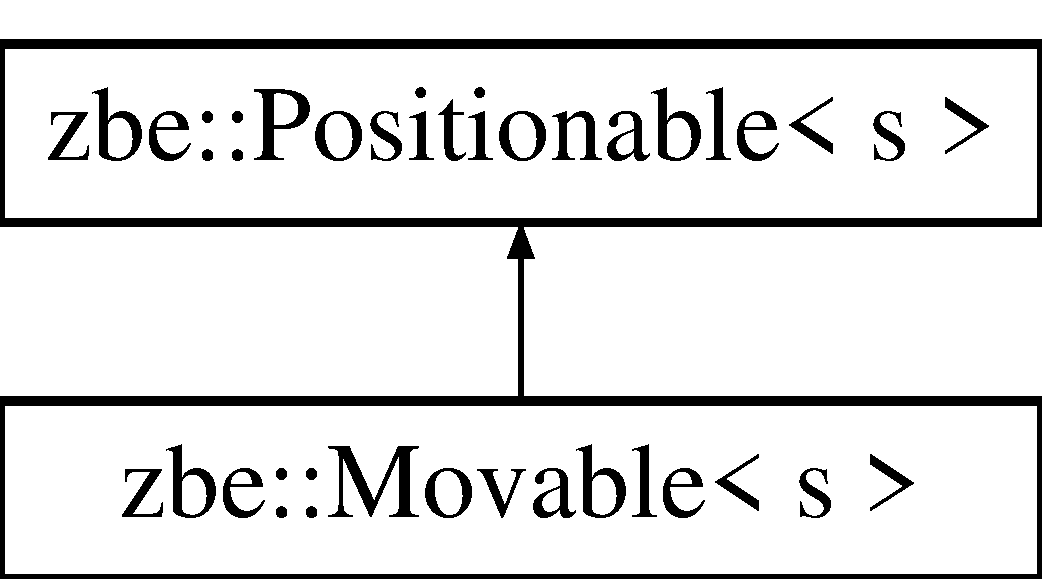
\includegraphics[height=2.000000cm]{classzbe_1_1_positionable}
\end{center}
\end{figure}
\subsection*{Public Member Functions}
\begin{DoxyCompactItemize}
\item 
\hyperlink{classzbe_1_1_positionable_a9fcb779fb35cc4d559177f240952aad8}{Positionable} ()
\item 
\hyperlink{classzbe_1_1_positionable_a6a11960f1a8d50a4f957908da1ea32a4}{Positionable} (\hyperlink{classzbe_1_1_point}{Point}$<$ s $>$ position)
\item 
virtual \hyperlink{classzbe_1_1_positionable_a8fbe13fe4d3ce705b3456f69222fb3b3}{$\sim$\+Positionable} ()
\item 
\hyperlink{classzbe_1_1_point}{Point}$<$ s $>$ \hyperlink{classzbe_1_1_positionable_abbce038018b1fe7d5c751334600f7287}{get\+Position} () const 
\item 
void \hyperlink{classzbe_1_1_positionable_a7667edc885aacd9c7f602f4e259c4ca5}{set\+Position} (\hyperlink{classzbe_1_1_point}{Point}$<$ s $>$ position)
\item 
void \hyperlink{classzbe_1_1_positionable_a728be26695a102a8c6b53142ab4509ef}{increase} (\hyperlink{classzbe_1_1_vector}{Vector}$<$ s $>$ offset)
\end{DoxyCompactItemize}


\subsection{Detailed Description}
\subsubsection*{template$<$unsigned s$>$class zbe\+::\+Positionable$<$ s $>$}



Definition at line 19 of file Positionable.\+h.



\subsection{Constructor \& Destructor Documentation}
\hypertarget{classzbe_1_1_positionable_a9fcb779fb35cc4d559177f240952aad8}{}\index{zbe\+::\+Positionable@{zbe\+::\+Positionable}!Positionable@{Positionable}}
\index{Positionable@{Positionable}!zbe\+::\+Positionable@{zbe\+::\+Positionable}}
\subsubsection[{Positionable()}]{\setlength{\rightskip}{0pt plus 5cm}template$<$unsigned s$>$ {\bf zbe\+::\+Positionable}$<$ s $>$\+::{\bf Positionable} (
\begin{DoxyParamCaption}
{}
\end{DoxyParamCaption}
)\hspace{0.3cm}{\ttfamily [inline]}}\label{classzbe_1_1_positionable_a9fcb779fb35cc4d559177f240952aad8}


Definition at line 21 of file Positionable.\+h.

\hypertarget{classzbe_1_1_positionable_a6a11960f1a8d50a4f957908da1ea32a4}{}\index{zbe\+::\+Positionable@{zbe\+::\+Positionable}!Positionable@{Positionable}}
\index{Positionable@{Positionable}!zbe\+::\+Positionable@{zbe\+::\+Positionable}}
\subsubsection[{Positionable(\+Point$<$ s $>$ position)}]{\setlength{\rightskip}{0pt plus 5cm}template$<$unsigned s$>$ {\bf zbe\+::\+Positionable}$<$ s $>$\+::{\bf Positionable} (
\begin{DoxyParamCaption}
\item[{{\bf Point}$<$ s $>$}]{position}
\end{DoxyParamCaption}
)\hspace{0.3cm}{\ttfamily [inline]}}\label{classzbe_1_1_positionable_a6a11960f1a8d50a4f957908da1ea32a4}


Definition at line 22 of file Positionable.\+h.

\hypertarget{classzbe_1_1_positionable_a8fbe13fe4d3ce705b3456f69222fb3b3}{}\index{zbe\+::\+Positionable@{zbe\+::\+Positionable}!````~Positionable@{$\sim$\+Positionable}}
\index{````~Positionable@{$\sim$\+Positionable}!zbe\+::\+Positionable@{zbe\+::\+Positionable}}
\subsubsection[{$\sim$\+Positionable()}]{\setlength{\rightskip}{0pt plus 5cm}template$<$unsigned s$>$ virtual {\bf zbe\+::\+Positionable}$<$ s $>$\+::$\sim${\bf Positionable} (
\begin{DoxyParamCaption}
{}
\end{DoxyParamCaption}
)\hspace{0.3cm}{\ttfamily [inline]}, {\ttfamily [virtual]}}\label{classzbe_1_1_positionable_a8fbe13fe4d3ce705b3456f69222fb3b3}


Definition at line 24 of file Positionable.\+h.



\subsection{Member Function Documentation}
\hypertarget{classzbe_1_1_positionable_abbce038018b1fe7d5c751334600f7287}{}\index{zbe\+::\+Positionable@{zbe\+::\+Positionable}!get\+Position@{get\+Position}}
\index{get\+Position@{get\+Position}!zbe\+::\+Positionable@{zbe\+::\+Positionable}}
\subsubsection[{get\+Position() const }]{\setlength{\rightskip}{0pt plus 5cm}template$<$unsigned s$>$ {\bf Point}$<$s$>$ {\bf zbe\+::\+Positionable}$<$ s $>$\+::get\+Position (
\begin{DoxyParamCaption}
{}
\end{DoxyParamCaption}
) const\hspace{0.3cm}{\ttfamily [inline]}}\label{classzbe_1_1_positionable_abbce038018b1fe7d5c751334600f7287}


Definition at line 26 of file Positionable.\+h.

\hypertarget{classzbe_1_1_positionable_a728be26695a102a8c6b53142ab4509ef}{}\index{zbe\+::\+Positionable@{zbe\+::\+Positionable}!increase@{increase}}
\index{increase@{increase}!zbe\+::\+Positionable@{zbe\+::\+Positionable}}
\subsubsection[{increase(\+Vector$<$ s $>$ offset)}]{\setlength{\rightskip}{0pt plus 5cm}template$<$unsigned s$>$ void {\bf zbe\+::\+Positionable}$<$ s $>$\+::increase (
\begin{DoxyParamCaption}
\item[{{\bf Vector}$<$ s $>$}]{offset}
\end{DoxyParamCaption}
)\hspace{0.3cm}{\ttfamily [inline]}}\label{classzbe_1_1_positionable_a728be26695a102a8c6b53142ab4509ef}


Definition at line 29 of file Positionable.\+h.

\hypertarget{classzbe_1_1_positionable_a7667edc885aacd9c7f602f4e259c4ca5}{}\index{zbe\+::\+Positionable@{zbe\+::\+Positionable}!set\+Position@{set\+Position}}
\index{set\+Position@{set\+Position}!zbe\+::\+Positionable@{zbe\+::\+Positionable}}
\subsubsection[{set\+Position(\+Point$<$ s $>$ position)}]{\setlength{\rightskip}{0pt plus 5cm}template$<$unsigned s$>$ void {\bf zbe\+::\+Positionable}$<$ s $>$\+::set\+Position (
\begin{DoxyParamCaption}
\item[{{\bf Point}$<$ s $>$}]{position}
\end{DoxyParamCaption}
)\hspace{0.3cm}{\ttfamily [inline]}}\label{classzbe_1_1_positionable_a7667edc885aacd9c7f602f4e259c4ca5}


Definition at line 27 of file Positionable.\+h.



The documentation for this class was generated from the following file\+:\begin{DoxyCompactItemize}
\item 
include/\+Z\+B\+E/core/archetypes/\hyperlink{_positionable_8h}{Positionable.\+h}\end{DoxyCompactItemize}

\hypertarget{structzbe_1_1_ray}{}\section{zbe\+:\+:Ray$<$ s $>$ Struct Template Reference}
\label{structzbe_1_1_ray}\index{zbe\+::\+Ray$<$ s $>$@{zbe\+::\+Ray$<$ s $>$}}


{\ttfamily \#include $<$objects.\+h$>$}

\subsection*{Public Member Functions}
\begin{DoxyCompactItemize}
\item 
\hyperlink{structzbe_1_1_ray_a5737d9d295af028eff8b86c7a9598173}{Ray} ()
\item 
\hyperlink{structzbe_1_1_ray_aa06cb424ee2e09cfe37ef3f3891622ae}{Ray} (\hyperlink{classzbe_1_1_point}{Point}$<$ s $>$ p, \hyperlink{classzbe_1_1_vector}{Vector}$<$ s $>$ v)
\item 
\hyperlink{structzbe_1_1_ray_a767a4a7c859d2227fe6c2c16733f9911}{Ray} (std\+::initializer\+\_\+list$<$ double $>$ lo, std\+::initializer\+\_\+list$<$ double $>$ lv)
\end{DoxyCompactItemize}
\subsection*{Public Attributes}
\begin{DoxyCompactItemize}
\item 
\hyperlink{classzbe_1_1_point}{Point}$<$ s $>$ \hyperlink{structzbe_1_1_ray_a156f5831d3d67cb661b6c8b64bd10546}{o}
\item 
\hyperlink{classzbe_1_1_vector}{Vector}$<$ s $>$ \hyperlink{structzbe_1_1_ray_a9b3d843a1155dc0746c3c28d0025b482}{d}
\end{DoxyCompactItemize}


\subsection{Detailed Description}
\subsubsection*{template$<$unsigned s$>$struct zbe\+::\+Ray$<$ s $>$}



Definition at line 21 of file objects.\+h.



\subsection{Constructor \& Destructor Documentation}
\hypertarget{structzbe_1_1_ray_a5737d9d295af028eff8b86c7a9598173}{}\index{zbe\+::\+Ray@{zbe\+::\+Ray}!Ray@{Ray}}
\index{Ray@{Ray}!zbe\+::\+Ray@{zbe\+::\+Ray}}
\subsubsection[{Ray()}]{\setlength{\rightskip}{0pt plus 5cm}template$<$unsigned s$>$ {\bf zbe\+::\+Ray}$<$ s $>$\+::{\bf Ray} (
\begin{DoxyParamCaption}
{}
\end{DoxyParamCaption}
)\hspace{0.3cm}{\ttfamily [inline]}}\label{structzbe_1_1_ray_a5737d9d295af028eff8b86c7a9598173}


Definition at line 22 of file objects.\+h.

\hypertarget{structzbe_1_1_ray_aa06cb424ee2e09cfe37ef3f3891622ae}{}\index{zbe\+::\+Ray@{zbe\+::\+Ray}!Ray@{Ray}}
\index{Ray@{Ray}!zbe\+::\+Ray@{zbe\+::\+Ray}}
\subsubsection[{Ray(\+Point$<$ s $>$ p, Vector$<$ s $>$ v)}]{\setlength{\rightskip}{0pt plus 5cm}template$<$unsigned s$>$ {\bf zbe\+::\+Ray}$<$ s $>$\+::{\bf Ray} (
\begin{DoxyParamCaption}
\item[{{\bf Point}$<$ s $>$}]{p, }
\item[{{\bf Vector}$<$ s $>$}]{v}
\end{DoxyParamCaption}
)\hspace{0.3cm}{\ttfamily [inline]}}\label{structzbe_1_1_ray_aa06cb424ee2e09cfe37ef3f3891622ae}


Definition at line 23 of file objects.\+h.

\hypertarget{structzbe_1_1_ray_a767a4a7c859d2227fe6c2c16733f9911}{}\index{zbe\+::\+Ray@{zbe\+::\+Ray}!Ray@{Ray}}
\index{Ray@{Ray}!zbe\+::\+Ray@{zbe\+::\+Ray}}
\subsubsection[{Ray(std\+::initializer\+\_\+list$<$ double $>$ lo, std\+::initializer\+\_\+list$<$ double $>$ lv)}]{\setlength{\rightskip}{0pt plus 5cm}template$<$unsigned s$>$ {\bf zbe\+::\+Ray}$<$ s $>$\+::{\bf Ray} (
\begin{DoxyParamCaption}
\item[{std\+::initializer\+\_\+list$<$ double $>$}]{lo, }
\item[{std\+::initializer\+\_\+list$<$ double $>$}]{lv}
\end{DoxyParamCaption}
)\hspace{0.3cm}{\ttfamily [inline]}}\label{structzbe_1_1_ray_a767a4a7c859d2227fe6c2c16733f9911}


Definition at line 24 of file objects.\+h.



\subsection{Member Data Documentation}
\hypertarget{structzbe_1_1_ray_a9b3d843a1155dc0746c3c28d0025b482}{}\index{zbe\+::\+Ray@{zbe\+::\+Ray}!d@{d}}
\index{d@{d}!zbe\+::\+Ray@{zbe\+::\+Ray}}
\subsubsection[{d}]{\setlength{\rightskip}{0pt plus 5cm}template$<$unsigned s$>$ {\bf Vector}$<$s$>$ {\bf zbe\+::\+Ray}$<$ s $>$\+::d}\label{structzbe_1_1_ray_a9b3d843a1155dc0746c3c28d0025b482}


Definition at line 27 of file objects.\+h.

\hypertarget{structzbe_1_1_ray_a156f5831d3d67cb661b6c8b64bd10546}{}\index{zbe\+::\+Ray@{zbe\+::\+Ray}!o@{o}}
\index{o@{o}!zbe\+::\+Ray@{zbe\+::\+Ray}}
\subsubsection[{o}]{\setlength{\rightskip}{0pt plus 5cm}template$<$unsigned s$>$ {\bf Point}$<$s$>$ {\bf zbe\+::\+Ray}$<$ s $>$\+::o}\label{structzbe_1_1_ray_a156f5831d3d67cb661b6c8b64bd10546}


Definition at line 26 of file objects.\+h.



The documentation for this struct was generated from the following file\+:\begin{DoxyCompactItemize}
\item 
include/\+Z\+B\+E/core/tools/math/\hyperlink{objects_8h}{objects.\+h}\end{DoxyCompactItemize}

\hypertarget{structzbe_1_1_ray2_d}{}\section{zbe\+:\+:Ray2\+D Struct Reference}
\label{structzbe_1_1_ray2_d}\index{zbe\+::\+Ray2\+D@{zbe\+::\+Ray2\+D}}


{\ttfamily \#include $<$objects.\+h$>$}

Inheritance diagram for zbe\+:\+:Ray2\+D\+:\begin{figure}[H]
\begin{center}
\leavevmode
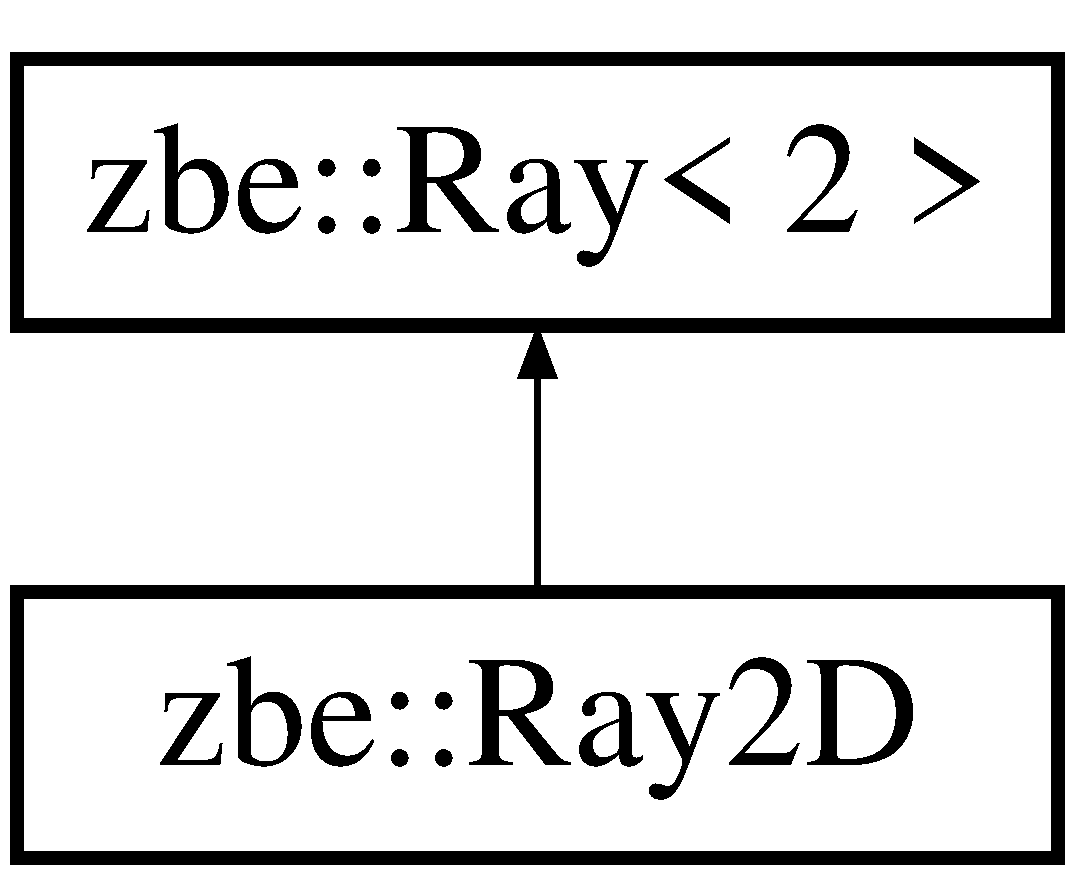
\includegraphics[height=2.000000cm]{structzbe_1_1_ray2_d}
\end{center}
\end{figure}
\subsection*{Public Member Functions}
\begin{DoxyCompactItemize}
\item 
\hyperlink{structzbe_1_1_ray2_d_aed7a0ed10788e292319d9008f1ac71b1}{Ray2\+D} ()
\item 
\hyperlink{structzbe_1_1_ray2_d_ac013ce11829eef5d663c135d6cfad339}{Ray2\+D} (\hyperlink{classzbe_1_1_point}{Point}$<$ 2 $>$ p, \hyperlink{classzbe_1_1_vector}{Vector}$<$ 2 $>$ v)
\item 
\hyperlink{structzbe_1_1_ray2_d_a69c7b3abf53ccbd453f12ec2785da112}{Ray2\+D} (std\+::initializer\+\_\+list$<$ double $>$ lo, std\+::initializer\+\_\+list$<$ double $>$ lv)
\end{DoxyCompactItemize}
\subsection*{Additional Inherited Members}


\subsection{Detailed Description}


Definition at line 31 of file objects.\+h.



\subsection{Constructor \& Destructor Documentation}
\hypertarget{structzbe_1_1_ray2_d_aed7a0ed10788e292319d9008f1ac71b1}{}\index{zbe\+::\+Ray2\+D@{zbe\+::\+Ray2\+D}!Ray2\+D@{Ray2\+D}}
\index{Ray2\+D@{Ray2\+D}!zbe\+::\+Ray2\+D@{zbe\+::\+Ray2\+D}}
\subsubsection[{Ray2\+D()}]{\setlength{\rightskip}{0pt plus 5cm}zbe\+::\+Ray2\+D\+::\+Ray2\+D (
\begin{DoxyParamCaption}
{}
\end{DoxyParamCaption}
)\hspace{0.3cm}{\ttfamily [inline]}}\label{structzbe_1_1_ray2_d_aed7a0ed10788e292319d9008f1ac71b1}


Definition at line 32 of file objects.\+h.

\hypertarget{structzbe_1_1_ray2_d_ac013ce11829eef5d663c135d6cfad339}{}\index{zbe\+::\+Ray2\+D@{zbe\+::\+Ray2\+D}!Ray2\+D@{Ray2\+D}}
\index{Ray2\+D@{Ray2\+D}!zbe\+::\+Ray2\+D@{zbe\+::\+Ray2\+D}}
\subsubsection[{Ray2\+D(\+Point$<$ 2 $>$ p, Vector$<$ 2 $>$ v)}]{\setlength{\rightskip}{0pt plus 5cm}zbe\+::\+Ray2\+D\+::\+Ray2\+D (
\begin{DoxyParamCaption}
\item[{{\bf Point}$<$ 2 $>$}]{p, }
\item[{{\bf Vector}$<$ 2 $>$}]{v}
\end{DoxyParamCaption}
)\hspace{0.3cm}{\ttfamily [inline]}}\label{structzbe_1_1_ray2_d_ac013ce11829eef5d663c135d6cfad339}


Definition at line 33 of file objects.\+h.

\hypertarget{structzbe_1_1_ray2_d_a69c7b3abf53ccbd453f12ec2785da112}{}\index{zbe\+::\+Ray2\+D@{zbe\+::\+Ray2\+D}!Ray2\+D@{Ray2\+D}}
\index{Ray2\+D@{Ray2\+D}!zbe\+::\+Ray2\+D@{zbe\+::\+Ray2\+D}}
\subsubsection[{Ray2\+D(std\+::initializer\+\_\+list$<$ double $>$ lo, std\+::initializer\+\_\+list$<$ double $>$ lv)}]{\setlength{\rightskip}{0pt plus 5cm}zbe\+::\+Ray2\+D\+::\+Ray2\+D (
\begin{DoxyParamCaption}
\item[{std\+::initializer\+\_\+list$<$ double $>$}]{lo, }
\item[{std\+::initializer\+\_\+list$<$ double $>$}]{lv}
\end{DoxyParamCaption}
)\hspace{0.3cm}{\ttfamily [inline]}}\label{structzbe_1_1_ray2_d_a69c7b3abf53ccbd453f12ec2785da112}


Definition at line 34 of file objects.\+h.



The documentation for this struct was generated from the following file\+:\begin{DoxyCompactItemize}
\item 
include/\+Z\+B\+E/core/tools/math/\hyperlink{objects_8h}{objects.\+h}\end{DoxyCompactItemize}

\hypertarget{structzbe_1_1_ray3_d}{}\section{zbe\+:\+:Ray3\+D Struct Reference}
\label{structzbe_1_1_ray3_d}\index{zbe\+::\+Ray3\+D@{zbe\+::\+Ray3\+D}}


{\ttfamily \#include $<$objects.\+h$>$}

Inheritance diagram for zbe\+:\+:Ray3\+D\+:\begin{figure}[H]
\begin{center}
\leavevmode
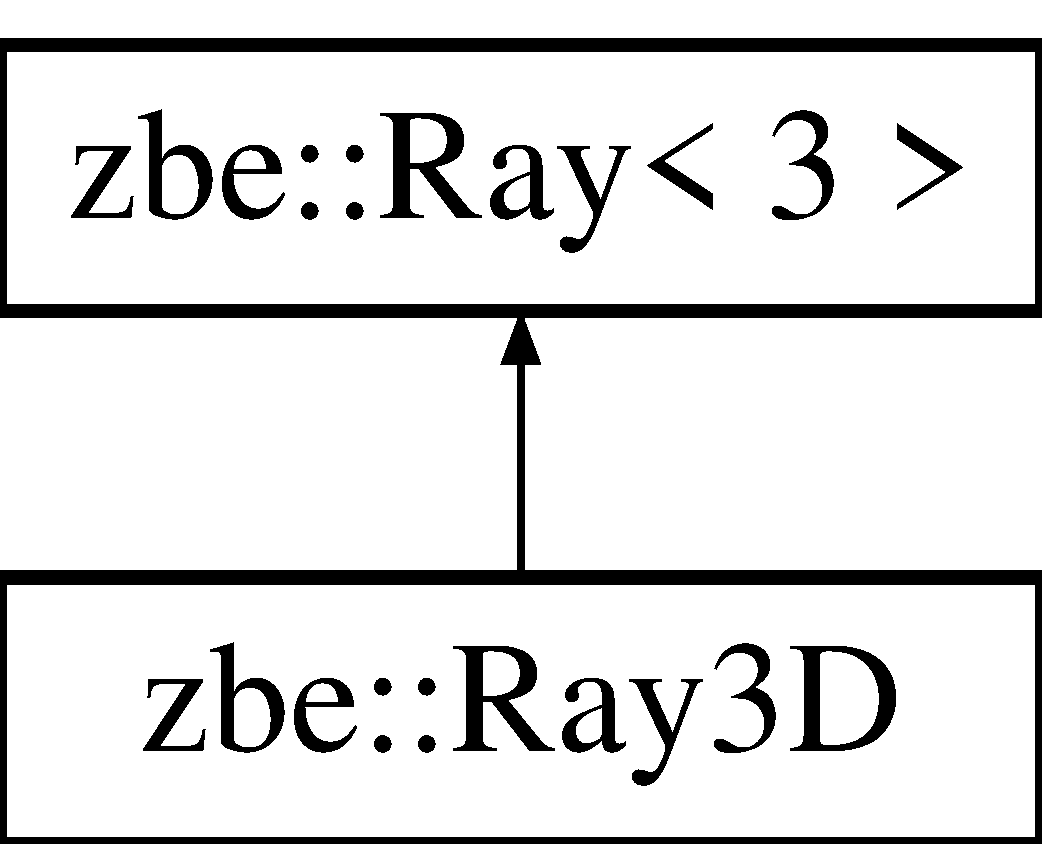
\includegraphics[height=2.000000cm]{structzbe_1_1_ray3_d}
\end{center}
\end{figure}
\subsection*{Public Member Functions}
\begin{DoxyCompactItemize}
\item 
\hyperlink{structzbe_1_1_ray3_d_aeacc9820d43cfcb0e421b16feeb8b7d0}{Ray3\+D} ()
\item 
\hyperlink{structzbe_1_1_ray3_d_a858eefb9eb400c570bed0b552c2ad633}{Ray3\+D} (\hyperlink{classzbe_1_1_point}{Point}$<$ 3 $>$ p, \hyperlink{classzbe_1_1_vector}{Vector}$<$ 3 $>$ v)
\item 
\hyperlink{structzbe_1_1_ray3_d_aed4225011d659fe8a913a940ace94833}{Ray3\+D} (std\+::initializer\+\_\+list$<$ double $>$ lo, std\+::initializer\+\_\+list$<$ double $>$ lv)
\end{DoxyCompactItemize}
\subsection*{Additional Inherited Members}


\subsection{Detailed Description}


Definition at line 37 of file objects.\+h.



\subsection{Constructor \& Destructor Documentation}
\hypertarget{structzbe_1_1_ray3_d_aeacc9820d43cfcb0e421b16feeb8b7d0}{}\index{zbe\+::\+Ray3\+D@{zbe\+::\+Ray3\+D}!Ray3\+D@{Ray3\+D}}
\index{Ray3\+D@{Ray3\+D}!zbe\+::\+Ray3\+D@{zbe\+::\+Ray3\+D}}
\subsubsection[{Ray3\+D()}]{\setlength{\rightskip}{0pt plus 5cm}zbe\+::\+Ray3\+D\+::\+Ray3\+D (
\begin{DoxyParamCaption}
{}
\end{DoxyParamCaption}
)\hspace{0.3cm}{\ttfamily [inline]}}\label{structzbe_1_1_ray3_d_aeacc9820d43cfcb0e421b16feeb8b7d0}


Definition at line 38 of file objects.\+h.

\hypertarget{structzbe_1_1_ray3_d_a858eefb9eb400c570bed0b552c2ad633}{}\index{zbe\+::\+Ray3\+D@{zbe\+::\+Ray3\+D}!Ray3\+D@{Ray3\+D}}
\index{Ray3\+D@{Ray3\+D}!zbe\+::\+Ray3\+D@{zbe\+::\+Ray3\+D}}
\subsubsection[{Ray3\+D(\+Point$<$ 3 $>$ p, Vector$<$ 3 $>$ v)}]{\setlength{\rightskip}{0pt plus 5cm}zbe\+::\+Ray3\+D\+::\+Ray3\+D (
\begin{DoxyParamCaption}
\item[{{\bf Point}$<$ 3 $>$}]{p, }
\item[{{\bf Vector}$<$ 3 $>$}]{v}
\end{DoxyParamCaption}
)\hspace{0.3cm}{\ttfamily [inline]}}\label{structzbe_1_1_ray3_d_a858eefb9eb400c570bed0b552c2ad633}


Definition at line 39 of file objects.\+h.

\hypertarget{structzbe_1_1_ray3_d_aed4225011d659fe8a913a940ace94833}{}\index{zbe\+::\+Ray3\+D@{zbe\+::\+Ray3\+D}!Ray3\+D@{Ray3\+D}}
\index{Ray3\+D@{Ray3\+D}!zbe\+::\+Ray3\+D@{zbe\+::\+Ray3\+D}}
\subsubsection[{Ray3\+D(std\+::initializer\+\_\+list$<$ double $>$ lo, std\+::initializer\+\_\+list$<$ double $>$ lv)}]{\setlength{\rightskip}{0pt plus 5cm}zbe\+::\+Ray3\+D\+::\+Ray3\+D (
\begin{DoxyParamCaption}
\item[{std\+::initializer\+\_\+list$<$ double $>$}]{lo, }
\item[{std\+::initializer\+\_\+list$<$ double $>$}]{lv}
\end{DoxyParamCaption}
)\hspace{0.3cm}{\ttfamily [inline]}}\label{structzbe_1_1_ray3_d_aed4225011d659fe8a913a940ace94833}


Definition at line 40 of file objects.\+h.



The documentation for this struct was generated from the following file\+:\begin{DoxyCompactItemize}
\item 
include/\+Z\+B\+E/core/tools/math/\hyperlink{objects_8h}{objects.\+h}\end{DoxyCompactItemize}

\hypertarget{classzbe_1_1_runnable}{}\section{zbe\+:\+:Runnable Class Reference}
\label{classzbe_1_1_runnable}\index{zbe\+::\+Runnable@{zbe\+::\+Runnable}}


{\ttfamily \#include $<$Runnable.\+h$>$}

Inheritance diagram for zbe\+:\+:Runnable\+:\begin{figure}[H]
\begin{center}
\leavevmode
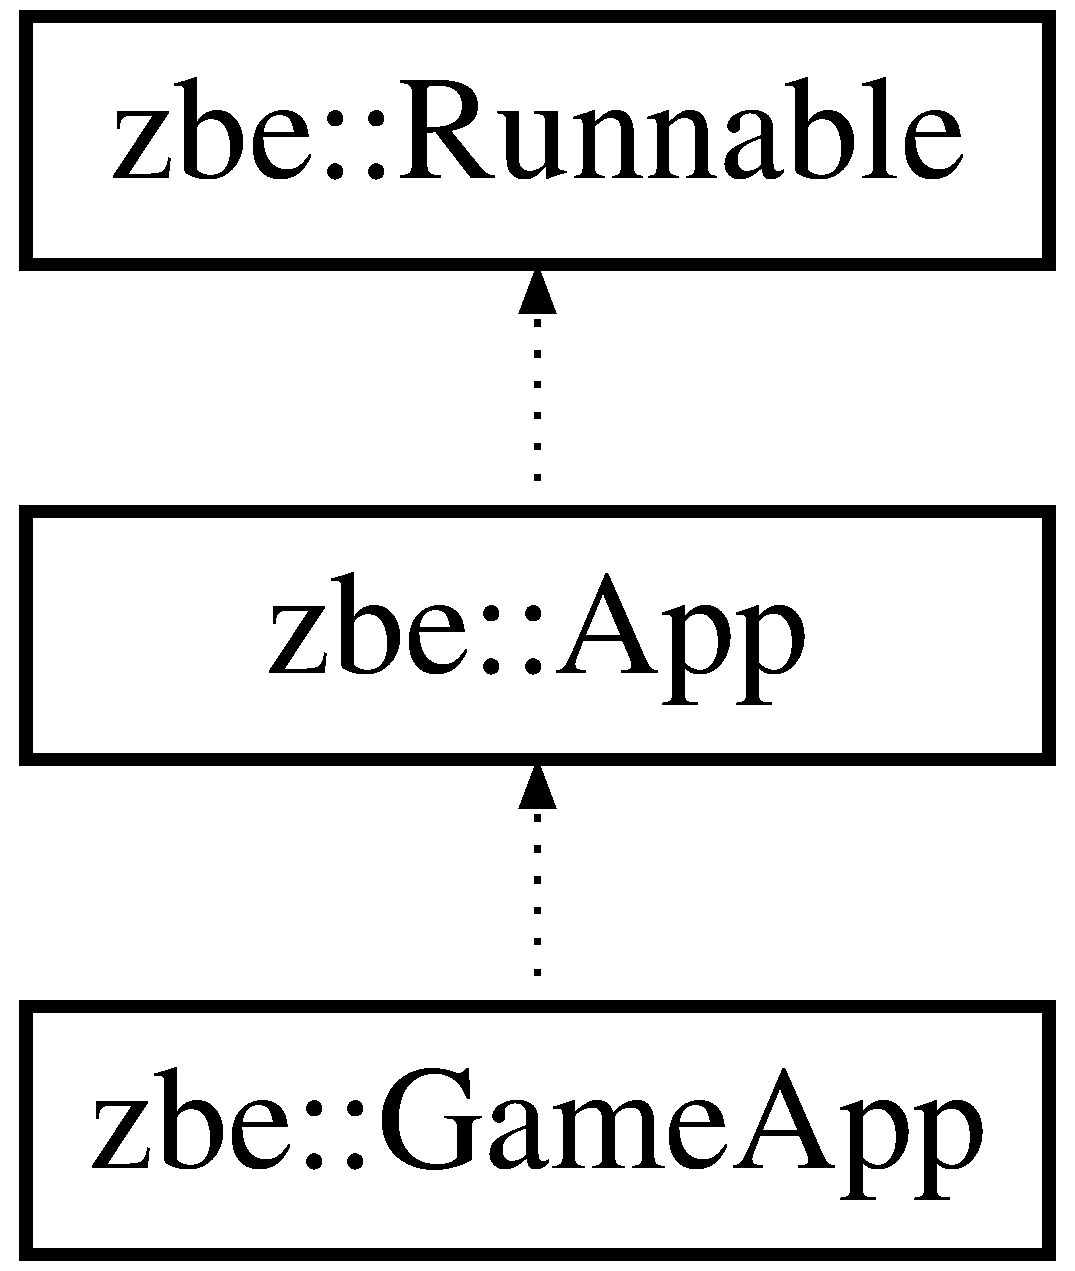
\includegraphics[height=3.000000cm]{classzbe_1_1_runnable}
\end{center}
\end{figure}
\subsection*{Public Member Functions}
\begin{DoxyCompactItemize}
\item 
virtual \hyperlink{classzbe_1_1_runnable_ab7e5b0a16122b190d09293f5a340032d}{$\sim$\+Runnable} ()
\item 
virtual void \hyperlink{classzbe_1_1_runnable_a9a1a946e8adefe5a291dfb7af74201d5}{run} ()=0
\end{DoxyCompactItemize}


\subsection{Detailed Description}


Definition at line 15 of file Runnable.\+h.



\subsection{Constructor \& Destructor Documentation}
\hypertarget{classzbe_1_1_runnable_ab7e5b0a16122b190d09293f5a340032d}{}\index{zbe\+::\+Runnable@{zbe\+::\+Runnable}!````~Runnable@{$\sim$\+Runnable}}
\index{````~Runnable@{$\sim$\+Runnable}!zbe\+::\+Runnable@{zbe\+::\+Runnable}}
\subsubsection[{$\sim$\+Runnable()}]{\setlength{\rightskip}{0pt plus 5cm}virtual zbe\+::\+Runnable\+::$\sim$\+Runnable (
\begin{DoxyParamCaption}
{}
\end{DoxyParamCaption}
)\hspace{0.3cm}{\ttfamily [inline]}, {\ttfamily [virtual]}}\label{classzbe_1_1_runnable_ab7e5b0a16122b190d09293f5a340032d}


Definition at line 17 of file Runnable.\+h.



\subsection{Member Function Documentation}
\hypertarget{classzbe_1_1_runnable_a9a1a946e8adefe5a291dfb7af74201d5}{}\index{zbe\+::\+Runnable@{zbe\+::\+Runnable}!run@{run}}
\index{run@{run}!zbe\+::\+Runnable@{zbe\+::\+Runnable}}
\subsubsection[{run()=0}]{\setlength{\rightskip}{0pt plus 5cm}virtual void zbe\+::\+Runnable\+::run (
\begin{DoxyParamCaption}
{}
\end{DoxyParamCaption}
)\hspace{0.3cm}{\ttfamily [pure virtual]}}\label{classzbe_1_1_runnable_a9a1a946e8adefe5a291dfb7af74201d5}


Implemented in \hyperlink{classzbe_1_1_app_ac952b75e2efcf5c2967da60dd95b57e6}{zbe\+::\+App}.



The documentation for this class was generated from the following file\+:\begin{DoxyCompactItemize}
\item 
include/\+Z\+B\+E/core/archetypes/\hyperlink{_runnable_8h}{Runnable.\+h}\end{DoxyCompactItemize}

\hypertarget{classzbe_1_1_s_d_l___starter}{}\section{zbe\+:\+:S\+D\+L\+\_\+\+Starter Class Reference}
\label{classzbe_1_1_s_d_l___starter}\index{zbe\+::\+S\+D\+L\+\_\+\+Starter@{zbe\+::\+S\+D\+L\+\_\+\+Starter}}


Used to init S\+D\+L subsystems only once (alonelton).  




{\ttfamily \#include $<$S\+D\+L\+\_\+\+Starter.\+h$>$}

\subsection*{Public Member Functions}
\begin{DoxyCompactItemize}
\item 
bool \hyperlink{classzbe_1_1_s_d_l___starter_a2a699a1cd9ee686fec81a491c0feef24}{add\+Subsystem} (Uint32 flags)
\end{DoxyCompactItemize}
\subsection*{Static Public Member Functions}
\begin{DoxyCompactItemize}
\item 
static \hyperlink{classzbe_1_1_s_d_l___starter}{S\+D\+L\+\_\+\+Starter} $\ast$ \hyperlink{classzbe_1_1_s_d_l___starter_a1ad467da339f54e91b446ccac984bb19}{create\+Instance} (Uint32 flags=0)
\item 
static void \hyperlink{classzbe_1_1_s_d_l___starter_ae14111197cb8103f36380d68bae78e98}{delete\+Instance} ()
\item 
static \hyperlink{classzbe_1_1_s_d_l___starter}{S\+D\+L\+\_\+\+Starter} $\ast$ \hyperlink{classzbe_1_1_s_d_l___starter_aca43aac3937f747d116d72e7e2374254}{get\+Instance} ()
\end{DoxyCompactItemize}


\subsection{Detailed Description}
Used to init S\+D\+L subsystems only once (alonelton). 

Definition at line 22 of file S\+D\+L\+\_\+\+Starter.\+h.



\subsection{Member Function Documentation}
\hypertarget{classzbe_1_1_s_d_l___starter_a2a699a1cd9ee686fec81a491c0feef24}{}\index{zbe\+::\+S\+D\+L\+\_\+\+Starter@{zbe\+::\+S\+D\+L\+\_\+\+Starter}!add\+Subsystem@{add\+Subsystem}}
\index{add\+Subsystem@{add\+Subsystem}!zbe\+::\+S\+D\+L\+\_\+\+Starter@{zbe\+::\+S\+D\+L\+\_\+\+Starter}}
\subsubsection[{add\+Subsystem(\+Uint32 flags)}]{\setlength{\rightskip}{0pt plus 5cm}bool zbe\+::\+S\+D\+L\+\_\+\+Starter\+::add\+Subsystem (
\begin{DoxyParamCaption}
\item[{Uint32}]{flags}
\end{DoxyParamCaption}
)}\label{classzbe_1_1_s_d_l___starter_a2a699a1cd9ee686fec81a491c0feef24}
\hypertarget{classzbe_1_1_s_d_l___starter_a1ad467da339f54e91b446ccac984bb19}{}\index{zbe\+::\+S\+D\+L\+\_\+\+Starter@{zbe\+::\+S\+D\+L\+\_\+\+Starter}!create\+Instance@{create\+Instance}}
\index{create\+Instance@{create\+Instance}!zbe\+::\+S\+D\+L\+\_\+\+Starter@{zbe\+::\+S\+D\+L\+\_\+\+Starter}}
\subsubsection[{create\+Instance(\+Uint32 flags=0)}]{\setlength{\rightskip}{0pt plus 5cm}static {\bf S\+D\+L\+\_\+\+Starter}$\ast$ zbe\+::\+S\+D\+L\+\_\+\+Starter\+::create\+Instance (
\begin{DoxyParamCaption}
\item[{Uint32}]{flags = {\ttfamily 0}}
\end{DoxyParamCaption}
)\hspace{0.3cm}{\ttfamily [static]}}\label{classzbe_1_1_s_d_l___starter_a1ad467da339f54e91b446ccac984bb19}
\hypertarget{classzbe_1_1_s_d_l___starter_ae14111197cb8103f36380d68bae78e98}{}\index{zbe\+::\+S\+D\+L\+\_\+\+Starter@{zbe\+::\+S\+D\+L\+\_\+\+Starter}!delete\+Instance@{delete\+Instance}}
\index{delete\+Instance@{delete\+Instance}!zbe\+::\+S\+D\+L\+\_\+\+Starter@{zbe\+::\+S\+D\+L\+\_\+\+Starter}}
\subsubsection[{delete\+Instance()}]{\setlength{\rightskip}{0pt plus 5cm}static void zbe\+::\+S\+D\+L\+\_\+\+Starter\+::delete\+Instance (
\begin{DoxyParamCaption}
{}
\end{DoxyParamCaption}
)\hspace{0.3cm}{\ttfamily [inline]}, {\ttfamily [static]}}\label{classzbe_1_1_s_d_l___starter_ae14111197cb8103f36380d68bae78e98}


Definition at line 25 of file S\+D\+L\+\_\+\+Starter.\+h.

\hypertarget{classzbe_1_1_s_d_l___starter_aca43aac3937f747d116d72e7e2374254}{}\index{zbe\+::\+S\+D\+L\+\_\+\+Starter@{zbe\+::\+S\+D\+L\+\_\+\+Starter}!get\+Instance@{get\+Instance}}
\index{get\+Instance@{get\+Instance}!zbe\+::\+S\+D\+L\+\_\+\+Starter@{zbe\+::\+S\+D\+L\+\_\+\+Starter}}
\subsubsection[{get\+Instance()}]{\setlength{\rightskip}{0pt plus 5cm}static {\bf S\+D\+L\+\_\+\+Starter}$\ast$ zbe\+::\+S\+D\+L\+\_\+\+Starter\+::get\+Instance (
\begin{DoxyParamCaption}
{}
\end{DoxyParamCaption}
)\hspace{0.3cm}{\ttfamily [inline]}, {\ttfamily [static]}}\label{classzbe_1_1_s_d_l___starter_aca43aac3937f747d116d72e7e2374254}


Definition at line 26 of file S\+D\+L\+\_\+\+Starter.\+h.



The documentation for this class was generated from the following file\+:\begin{DoxyCompactItemize}
\item 
include/\+Z\+B\+E/core/starters/\hyperlink{_s_d_l___starter_8h}{S\+D\+L\+\_\+\+Starter.\+h}\end{DoxyCompactItemize}

\hypertarget{classzbe_1_1_s_d_l_font_loader}{}\section{zbe\+:\+:S\+D\+L\+Font\+Loader Class Reference}
\label{classzbe_1_1_s_d_l_font_loader}\index{zbe\+::\+S\+D\+L\+Font\+Loader@{zbe\+::\+S\+D\+L\+Font\+Loader}}


{\ttfamily \#include $<$S\+D\+L\+Font\+Loader.\+h$>$}

\subsection*{Public Member Functions}
\begin{DoxyCompactItemize}
\item 
void \hyperlink{classzbe_1_1_s_d_l_font_loader_a0a6e10fecc8e6fe5fa419c5ec1aa7e8a}{load\+Font} (const char $\ast$url, int size, int id)
\item 
void \hyperlink{classzbe_1_1_s_d_l_font_loader_a997b0661f40f21fabbae138731ee9661}{reload\+Font} (const char $\ast$url, int size, int id)
\item 
void \hyperlink{classzbe_1_1_s_d_l_font_loader_a095cf2b0d87f453a25a9b25a37516edd}{remove\+Font} (int id)
\item 
T\+T\+F\+\_\+\+Font $\ast$ \hyperlink{classzbe_1_1_s_d_l_font_loader_af238cc377c43f0fe4d9601ee4aabc80b}{get\+Font} (int id)
\end{DoxyCompactItemize}
\subsection*{Static Public Member Functions}
\begin{DoxyCompactItemize}
\item 
static \hyperlink{classzbe_1_1_s_d_l_font_loader}{S\+D\+L\+Font\+Loader} $\ast$ \hyperlink{classzbe_1_1_s_d_l_font_loader_aa6c4b5b2c7338f6c58b6df3973e59c69}{create\+Instance} ()
\item 
static void \hyperlink{classzbe_1_1_s_d_l_font_loader_a62c91e48397c42e78ea18ff052c79e38}{delete\+Instance} ()
\item 
static \hyperlink{classzbe_1_1_s_d_l_font_loader}{S\+D\+L\+Font\+Loader} $\ast$ \hyperlink{classzbe_1_1_s_d_l_font_loader_a5627540479115934fab1832fa0f0e785}{get\+Instance} ()
\end{DoxyCompactItemize}


\subsection{Detailed Description}


Definition at line 22 of file S\+D\+L\+Font\+Loader.\+h.



\subsection{Member Function Documentation}
\hypertarget{classzbe_1_1_s_d_l_font_loader_aa6c4b5b2c7338f6c58b6df3973e59c69}{}\index{zbe\+::\+S\+D\+L\+Font\+Loader@{zbe\+::\+S\+D\+L\+Font\+Loader}!create\+Instance@{create\+Instance}}
\index{create\+Instance@{create\+Instance}!zbe\+::\+S\+D\+L\+Font\+Loader@{zbe\+::\+S\+D\+L\+Font\+Loader}}
\subsubsection[{create\+Instance()}]{\setlength{\rightskip}{0pt plus 5cm}static {\bf S\+D\+L\+Font\+Loader}$\ast$ zbe\+::\+S\+D\+L\+Font\+Loader\+::create\+Instance (
\begin{DoxyParamCaption}
{}
\end{DoxyParamCaption}
)\hspace{0.3cm}{\ttfamily [static]}}\label{classzbe_1_1_s_d_l_font_loader_aa6c4b5b2c7338f6c58b6df3973e59c69}
\hypertarget{classzbe_1_1_s_d_l_font_loader_a62c91e48397c42e78ea18ff052c79e38}{}\index{zbe\+::\+S\+D\+L\+Font\+Loader@{zbe\+::\+S\+D\+L\+Font\+Loader}!delete\+Instance@{delete\+Instance}}
\index{delete\+Instance@{delete\+Instance}!zbe\+::\+S\+D\+L\+Font\+Loader@{zbe\+::\+S\+D\+L\+Font\+Loader}}
\subsubsection[{delete\+Instance()}]{\setlength{\rightskip}{0pt plus 5cm}static void zbe\+::\+S\+D\+L\+Font\+Loader\+::delete\+Instance (
\begin{DoxyParamCaption}
{}
\end{DoxyParamCaption}
)\hspace{0.3cm}{\ttfamily [static]}}\label{classzbe_1_1_s_d_l_font_loader_a62c91e48397c42e78ea18ff052c79e38}
\hypertarget{classzbe_1_1_s_d_l_font_loader_af238cc377c43f0fe4d9601ee4aabc80b}{}\index{zbe\+::\+S\+D\+L\+Font\+Loader@{zbe\+::\+S\+D\+L\+Font\+Loader}!get\+Font@{get\+Font}}
\index{get\+Font@{get\+Font}!zbe\+::\+S\+D\+L\+Font\+Loader@{zbe\+::\+S\+D\+L\+Font\+Loader}}
\subsubsection[{get\+Font(int id)}]{\setlength{\rightskip}{0pt plus 5cm}T\+T\+F\+\_\+\+Font$\ast$ zbe\+::\+S\+D\+L\+Font\+Loader\+::get\+Font (
\begin{DoxyParamCaption}
\item[{int}]{id}
\end{DoxyParamCaption}
)}\label{classzbe_1_1_s_d_l_font_loader_af238cc377c43f0fe4d9601ee4aabc80b}
\hypertarget{classzbe_1_1_s_d_l_font_loader_a5627540479115934fab1832fa0f0e785}{}\index{zbe\+::\+S\+D\+L\+Font\+Loader@{zbe\+::\+S\+D\+L\+Font\+Loader}!get\+Instance@{get\+Instance}}
\index{get\+Instance@{get\+Instance}!zbe\+::\+S\+D\+L\+Font\+Loader@{zbe\+::\+S\+D\+L\+Font\+Loader}}
\subsubsection[{get\+Instance()}]{\setlength{\rightskip}{0pt plus 5cm}static {\bf S\+D\+L\+Font\+Loader}$\ast$ zbe\+::\+S\+D\+L\+Font\+Loader\+::get\+Instance (
\begin{DoxyParamCaption}
{}
\end{DoxyParamCaption}
)\hspace{0.3cm}{\ttfamily [static]}}\label{classzbe_1_1_s_d_l_font_loader_a5627540479115934fab1832fa0f0e785}
\hypertarget{classzbe_1_1_s_d_l_font_loader_a0a6e10fecc8e6fe5fa419c5ec1aa7e8a}{}\index{zbe\+::\+S\+D\+L\+Font\+Loader@{zbe\+::\+S\+D\+L\+Font\+Loader}!load\+Font@{load\+Font}}
\index{load\+Font@{load\+Font}!zbe\+::\+S\+D\+L\+Font\+Loader@{zbe\+::\+S\+D\+L\+Font\+Loader}}
\subsubsection[{load\+Font(const char $\ast$url, int size, int id)}]{\setlength{\rightskip}{0pt plus 5cm}void zbe\+::\+S\+D\+L\+Font\+Loader\+::load\+Font (
\begin{DoxyParamCaption}
\item[{const char $\ast$}]{url, }
\item[{int}]{size, }
\item[{int}]{id}
\end{DoxyParamCaption}
)}\label{classzbe_1_1_s_d_l_font_loader_a0a6e10fecc8e6fe5fa419c5ec1aa7e8a}
\hypertarget{classzbe_1_1_s_d_l_font_loader_a997b0661f40f21fabbae138731ee9661}{}\index{zbe\+::\+S\+D\+L\+Font\+Loader@{zbe\+::\+S\+D\+L\+Font\+Loader}!reload\+Font@{reload\+Font}}
\index{reload\+Font@{reload\+Font}!zbe\+::\+S\+D\+L\+Font\+Loader@{zbe\+::\+S\+D\+L\+Font\+Loader}}
\subsubsection[{reload\+Font(const char $\ast$url, int size, int id)}]{\setlength{\rightskip}{0pt plus 5cm}void zbe\+::\+S\+D\+L\+Font\+Loader\+::reload\+Font (
\begin{DoxyParamCaption}
\item[{const char $\ast$}]{url, }
\item[{int}]{size, }
\item[{int}]{id}
\end{DoxyParamCaption}
)}\label{classzbe_1_1_s_d_l_font_loader_a997b0661f40f21fabbae138731ee9661}
\hypertarget{classzbe_1_1_s_d_l_font_loader_a095cf2b0d87f453a25a9b25a37516edd}{}\index{zbe\+::\+S\+D\+L\+Font\+Loader@{zbe\+::\+S\+D\+L\+Font\+Loader}!remove\+Font@{remove\+Font}}
\index{remove\+Font@{remove\+Font}!zbe\+::\+S\+D\+L\+Font\+Loader@{zbe\+::\+S\+D\+L\+Font\+Loader}}
\subsubsection[{remove\+Font(int id)}]{\setlength{\rightskip}{0pt plus 5cm}void zbe\+::\+S\+D\+L\+Font\+Loader\+::remove\+Font (
\begin{DoxyParamCaption}
\item[{int}]{id}
\end{DoxyParamCaption}
)}\label{classzbe_1_1_s_d_l_font_loader_a095cf2b0d87f453a25a9b25a37516edd}


The documentation for this class was generated from the following file\+:\begin{DoxyCompactItemize}
\item 
include/\+Z\+B\+E/core/loaders/\hyperlink{_s_d_l_font_loader_8h}{S\+D\+L\+Font\+Loader.\+h}\end{DoxyCompactItemize}

\hypertarget{classzbe_1_1_simple_sprite}{}\section{zbe\+:\+:Simple\+Sprite Class Reference}
\label{classzbe_1_1_simple_sprite}\index{zbe\+::\+Simple\+Sprite@{zbe\+::\+Simple\+Sprite}}


{\ttfamily \#include $<$Simple\+Sprite.\+h$>$}

\subsection*{Public Member Functions}
\begin{DoxyCompactItemize}
\item 
\hyperlink{classzbe_1_1_simple_sprite_aa69fa08ed54f96fccf9ee6c7f23e87a1}{Simple\+Sprite} ()
\item 
\hyperlink{classzbe_1_1_simple_sprite_a7b58550af6e09561d35a03b5bb66a9b3}{Simple\+Sprite} (unsigned width, unsigned height, unsigned img)
\item 
\hyperlink{classzbe_1_1_simple_sprite_a187547fd761f559c97a2d4d95c8da277}{Simple\+Sprite} (int x, int y, unsigned width, unsigned height, unsigned img)
\item 
\hyperlink{classzbe_1_1_simple_sprite_ab11cf4d8abd2624165472efe7846615b}{$\sim$\+Simple\+Sprite} ()
\item 
void \hyperlink{classzbe_1_1_simple_sprite_afb93da780f6e1bca773c5026ce5045b7}{set\+Left\+X} (int x)
\item 
void \hyperlink{classzbe_1_1_simple_sprite_a03726cc6ded8ae30351cae031702aed3}{set\+Top\+Y} (int y)
\item 
void \hyperlink{classzbe_1_1_simple_sprite_aa5758be3c6bc1e13cdd69861ca48f8ce}{set\+Width} (unsigned width)
\item 
void \hyperlink{classzbe_1_1_simple_sprite_a0fb0a122ee902c9dd34945bf926e0899}{set\+Height} (unsigned height)
\item 
void \hyperlink{classzbe_1_1_simple_sprite_a0bc876cc324b11968a4decb241ae521c}{set\+Image} (unsigned img)
\item 
int \hyperlink{classzbe_1_1_simple_sprite_a031c01a6cc162b01113107b345aeaa61}{get\+Left\+X} () const 
\item 
int \hyperlink{classzbe_1_1_simple_sprite_af004923d23cb1ea3f3cf851b47a88562}{get\+Top\+Y} () const 
\item 
unsigned \hyperlink{classzbe_1_1_simple_sprite_aba0207ed8eb791d9300a5eafe55ef1a7}{get\+Width} () const 
\item 
unsigned \hyperlink{classzbe_1_1_simple_sprite_ae42bad4677f86bc86cb61c5a0f9c8c51}{get\+Height} () const 
\item 
unsigned \hyperlink{classzbe_1_1_simple_sprite_af9654d9a43b9faec87285c116f595c0d}{get\+Image} () const 
\end{DoxyCompactItemize}


\subsection{Detailed Description}


Definition at line 17 of file Simple\+Sprite.\+h.



\subsection{Constructor \& Destructor Documentation}
\hypertarget{classzbe_1_1_simple_sprite_aa69fa08ed54f96fccf9ee6c7f23e87a1}{}\index{zbe\+::\+Simple\+Sprite@{zbe\+::\+Simple\+Sprite}!Simple\+Sprite@{Simple\+Sprite}}
\index{Simple\+Sprite@{Simple\+Sprite}!zbe\+::\+Simple\+Sprite@{zbe\+::\+Simple\+Sprite}}
\subsubsection[{Simple\+Sprite()}]{\setlength{\rightskip}{0pt plus 5cm}zbe\+::\+Simple\+Sprite\+::\+Simple\+Sprite (
\begin{DoxyParamCaption}
{}
\end{DoxyParamCaption}
)\hspace{0.3cm}{\ttfamily [inline]}}\label{classzbe_1_1_simple_sprite_aa69fa08ed54f96fccf9ee6c7f23e87a1}


Definition at line 19 of file Simple\+Sprite.\+h.

\hypertarget{classzbe_1_1_simple_sprite_a7b58550af6e09561d35a03b5bb66a9b3}{}\index{zbe\+::\+Simple\+Sprite@{zbe\+::\+Simple\+Sprite}!Simple\+Sprite@{Simple\+Sprite}}
\index{Simple\+Sprite@{Simple\+Sprite}!zbe\+::\+Simple\+Sprite@{zbe\+::\+Simple\+Sprite}}
\subsubsection[{Simple\+Sprite(unsigned width, unsigned height, unsigned img)}]{\setlength{\rightskip}{0pt plus 5cm}zbe\+::\+Simple\+Sprite\+::\+Simple\+Sprite (
\begin{DoxyParamCaption}
\item[{unsigned}]{width, }
\item[{unsigned}]{height, }
\item[{unsigned}]{img}
\end{DoxyParamCaption}
)\hspace{0.3cm}{\ttfamily [inline]}}\label{classzbe_1_1_simple_sprite_a7b58550af6e09561d35a03b5bb66a9b3}


Definition at line 20 of file Simple\+Sprite.\+h.

\hypertarget{classzbe_1_1_simple_sprite_a187547fd761f559c97a2d4d95c8da277}{}\index{zbe\+::\+Simple\+Sprite@{zbe\+::\+Simple\+Sprite}!Simple\+Sprite@{Simple\+Sprite}}
\index{Simple\+Sprite@{Simple\+Sprite}!zbe\+::\+Simple\+Sprite@{zbe\+::\+Simple\+Sprite}}
\subsubsection[{Simple\+Sprite(int x, int y, unsigned width, unsigned height, unsigned img)}]{\setlength{\rightskip}{0pt plus 5cm}zbe\+::\+Simple\+Sprite\+::\+Simple\+Sprite (
\begin{DoxyParamCaption}
\item[{int}]{x, }
\item[{int}]{y, }
\item[{unsigned}]{width, }
\item[{unsigned}]{height, }
\item[{unsigned}]{img}
\end{DoxyParamCaption}
)\hspace{0.3cm}{\ttfamily [inline]}}\label{classzbe_1_1_simple_sprite_a187547fd761f559c97a2d4d95c8da277}


Definition at line 21 of file Simple\+Sprite.\+h.

\hypertarget{classzbe_1_1_simple_sprite_ab11cf4d8abd2624165472efe7846615b}{}\index{zbe\+::\+Simple\+Sprite@{zbe\+::\+Simple\+Sprite}!````~Simple\+Sprite@{$\sim$\+Simple\+Sprite}}
\index{````~Simple\+Sprite@{$\sim$\+Simple\+Sprite}!zbe\+::\+Simple\+Sprite@{zbe\+::\+Simple\+Sprite}}
\subsubsection[{$\sim$\+Simple\+Sprite()}]{\setlength{\rightskip}{0pt plus 5cm}zbe\+::\+Simple\+Sprite\+::$\sim$\+Simple\+Sprite (
\begin{DoxyParamCaption}
{}
\end{DoxyParamCaption}
)\hspace{0.3cm}{\ttfamily [inline]}}\label{classzbe_1_1_simple_sprite_ab11cf4d8abd2624165472efe7846615b}


Definition at line 23 of file Simple\+Sprite.\+h.



\subsection{Member Function Documentation}
\hypertarget{classzbe_1_1_simple_sprite_ae42bad4677f86bc86cb61c5a0f9c8c51}{}\index{zbe\+::\+Simple\+Sprite@{zbe\+::\+Simple\+Sprite}!get\+Height@{get\+Height}}
\index{get\+Height@{get\+Height}!zbe\+::\+Simple\+Sprite@{zbe\+::\+Simple\+Sprite}}
\subsubsection[{get\+Height() const }]{\setlength{\rightskip}{0pt plus 5cm}unsigned zbe\+::\+Simple\+Sprite\+::get\+Height (
\begin{DoxyParamCaption}
{}
\end{DoxyParamCaption}
) const\hspace{0.3cm}{\ttfamily [inline]}}\label{classzbe_1_1_simple_sprite_ae42bad4677f86bc86cb61c5a0f9c8c51}


Definition at line 34 of file Simple\+Sprite.\+h.

\hypertarget{classzbe_1_1_simple_sprite_af9654d9a43b9faec87285c116f595c0d}{}\index{zbe\+::\+Simple\+Sprite@{zbe\+::\+Simple\+Sprite}!get\+Image@{get\+Image}}
\index{get\+Image@{get\+Image}!zbe\+::\+Simple\+Sprite@{zbe\+::\+Simple\+Sprite}}
\subsubsection[{get\+Image() const }]{\setlength{\rightskip}{0pt plus 5cm}unsigned zbe\+::\+Simple\+Sprite\+::get\+Image (
\begin{DoxyParamCaption}
{}
\end{DoxyParamCaption}
) const\hspace{0.3cm}{\ttfamily [inline]}}\label{classzbe_1_1_simple_sprite_af9654d9a43b9faec87285c116f595c0d}


Definition at line 35 of file Simple\+Sprite.\+h.

\hypertarget{classzbe_1_1_simple_sprite_a031c01a6cc162b01113107b345aeaa61}{}\index{zbe\+::\+Simple\+Sprite@{zbe\+::\+Simple\+Sprite}!get\+Left\+X@{get\+Left\+X}}
\index{get\+Left\+X@{get\+Left\+X}!zbe\+::\+Simple\+Sprite@{zbe\+::\+Simple\+Sprite}}
\subsubsection[{get\+Left\+X() const }]{\setlength{\rightskip}{0pt plus 5cm}int zbe\+::\+Simple\+Sprite\+::get\+Left\+X (
\begin{DoxyParamCaption}
{}
\end{DoxyParamCaption}
) const\hspace{0.3cm}{\ttfamily [inline]}}\label{classzbe_1_1_simple_sprite_a031c01a6cc162b01113107b345aeaa61}


Definition at line 31 of file Simple\+Sprite.\+h.

\hypertarget{classzbe_1_1_simple_sprite_af004923d23cb1ea3f3cf851b47a88562}{}\index{zbe\+::\+Simple\+Sprite@{zbe\+::\+Simple\+Sprite}!get\+Top\+Y@{get\+Top\+Y}}
\index{get\+Top\+Y@{get\+Top\+Y}!zbe\+::\+Simple\+Sprite@{zbe\+::\+Simple\+Sprite}}
\subsubsection[{get\+Top\+Y() const }]{\setlength{\rightskip}{0pt plus 5cm}int zbe\+::\+Simple\+Sprite\+::get\+Top\+Y (
\begin{DoxyParamCaption}
{}
\end{DoxyParamCaption}
) const\hspace{0.3cm}{\ttfamily [inline]}}\label{classzbe_1_1_simple_sprite_af004923d23cb1ea3f3cf851b47a88562}


Definition at line 32 of file Simple\+Sprite.\+h.

\hypertarget{classzbe_1_1_simple_sprite_aba0207ed8eb791d9300a5eafe55ef1a7}{}\index{zbe\+::\+Simple\+Sprite@{zbe\+::\+Simple\+Sprite}!get\+Width@{get\+Width}}
\index{get\+Width@{get\+Width}!zbe\+::\+Simple\+Sprite@{zbe\+::\+Simple\+Sprite}}
\subsubsection[{get\+Width() const }]{\setlength{\rightskip}{0pt plus 5cm}unsigned zbe\+::\+Simple\+Sprite\+::get\+Width (
\begin{DoxyParamCaption}
{}
\end{DoxyParamCaption}
) const\hspace{0.3cm}{\ttfamily [inline]}}\label{classzbe_1_1_simple_sprite_aba0207ed8eb791d9300a5eafe55ef1a7}


Definition at line 33 of file Simple\+Sprite.\+h.

\hypertarget{classzbe_1_1_simple_sprite_a0fb0a122ee902c9dd34945bf926e0899}{}\index{zbe\+::\+Simple\+Sprite@{zbe\+::\+Simple\+Sprite}!set\+Height@{set\+Height}}
\index{set\+Height@{set\+Height}!zbe\+::\+Simple\+Sprite@{zbe\+::\+Simple\+Sprite}}
\subsubsection[{set\+Height(unsigned height)}]{\setlength{\rightskip}{0pt plus 5cm}void zbe\+::\+Simple\+Sprite\+::set\+Height (
\begin{DoxyParamCaption}
\item[{unsigned}]{height}
\end{DoxyParamCaption}
)\hspace{0.3cm}{\ttfamily [inline]}}\label{classzbe_1_1_simple_sprite_a0fb0a122ee902c9dd34945bf926e0899}


Definition at line 28 of file Simple\+Sprite.\+h.

\hypertarget{classzbe_1_1_simple_sprite_a0bc876cc324b11968a4decb241ae521c}{}\index{zbe\+::\+Simple\+Sprite@{zbe\+::\+Simple\+Sprite}!set\+Image@{set\+Image}}
\index{set\+Image@{set\+Image}!zbe\+::\+Simple\+Sprite@{zbe\+::\+Simple\+Sprite}}
\subsubsection[{set\+Image(unsigned img)}]{\setlength{\rightskip}{0pt plus 5cm}void zbe\+::\+Simple\+Sprite\+::set\+Image (
\begin{DoxyParamCaption}
\item[{unsigned}]{img}
\end{DoxyParamCaption}
)\hspace{0.3cm}{\ttfamily [inline]}}\label{classzbe_1_1_simple_sprite_a0bc876cc324b11968a4decb241ae521c}


Definition at line 29 of file Simple\+Sprite.\+h.

\hypertarget{classzbe_1_1_simple_sprite_afb93da780f6e1bca773c5026ce5045b7}{}\index{zbe\+::\+Simple\+Sprite@{zbe\+::\+Simple\+Sprite}!set\+Left\+X@{set\+Left\+X}}
\index{set\+Left\+X@{set\+Left\+X}!zbe\+::\+Simple\+Sprite@{zbe\+::\+Simple\+Sprite}}
\subsubsection[{set\+Left\+X(int x)}]{\setlength{\rightskip}{0pt plus 5cm}void zbe\+::\+Simple\+Sprite\+::set\+Left\+X (
\begin{DoxyParamCaption}
\item[{int}]{x}
\end{DoxyParamCaption}
)\hspace{0.3cm}{\ttfamily [inline]}}\label{classzbe_1_1_simple_sprite_afb93da780f6e1bca773c5026ce5045b7}


Definition at line 25 of file Simple\+Sprite.\+h.

\hypertarget{classzbe_1_1_simple_sprite_a03726cc6ded8ae30351cae031702aed3}{}\index{zbe\+::\+Simple\+Sprite@{zbe\+::\+Simple\+Sprite}!set\+Top\+Y@{set\+Top\+Y}}
\index{set\+Top\+Y@{set\+Top\+Y}!zbe\+::\+Simple\+Sprite@{zbe\+::\+Simple\+Sprite}}
\subsubsection[{set\+Top\+Y(int y)}]{\setlength{\rightskip}{0pt plus 5cm}void zbe\+::\+Simple\+Sprite\+::set\+Top\+Y (
\begin{DoxyParamCaption}
\item[{int}]{y}
\end{DoxyParamCaption}
)\hspace{0.3cm}{\ttfamily [inline]}}\label{classzbe_1_1_simple_sprite_a03726cc6ded8ae30351cae031702aed3}


Definition at line 26 of file Simple\+Sprite.\+h.

\hypertarget{classzbe_1_1_simple_sprite_aa5758be3c6bc1e13cdd69861ca48f8ce}{}\index{zbe\+::\+Simple\+Sprite@{zbe\+::\+Simple\+Sprite}!set\+Width@{set\+Width}}
\index{set\+Width@{set\+Width}!zbe\+::\+Simple\+Sprite@{zbe\+::\+Simple\+Sprite}}
\subsubsection[{set\+Width(unsigned width)}]{\setlength{\rightskip}{0pt plus 5cm}void zbe\+::\+Simple\+Sprite\+::set\+Width (
\begin{DoxyParamCaption}
\item[{unsigned}]{width}
\end{DoxyParamCaption}
)\hspace{0.3cm}{\ttfamily [inline]}}\label{classzbe_1_1_simple_sprite_aa5758be3c6bc1e13cdd69861ca48f8ce}


Definition at line 27 of file Simple\+Sprite.\+h.



The documentation for this class was generated from the following file\+:\begin{DoxyCompactItemize}
\item 
include/\+Z\+B\+E/core/archetypes/\hyperlink{_simple_sprite_8h}{Simple\+Sprite.\+h}\end{DoxyCompactItemize}

\hypertarget{classzbe_1_1_simple_sprite_s_d_l_drawer}{}\section{zbe\+:\+:Simple\+Sprite\+S\+D\+L\+Drawer Class Reference}
\label{classzbe_1_1_simple_sprite_s_d_l_drawer}\index{zbe\+::\+Simple\+Sprite\+S\+D\+L\+Drawer@{zbe\+::\+Simple\+Sprite\+S\+D\+L\+Drawer}}


{\ttfamily \#include $<$Simple\+Sprite\+S\+D\+L\+Drawer.\+h$>$}

Inheritance diagram for zbe\+:\+:Simple\+Sprite\+S\+D\+L\+Drawer\+:\begin{figure}[H]
\begin{center}
\leavevmode
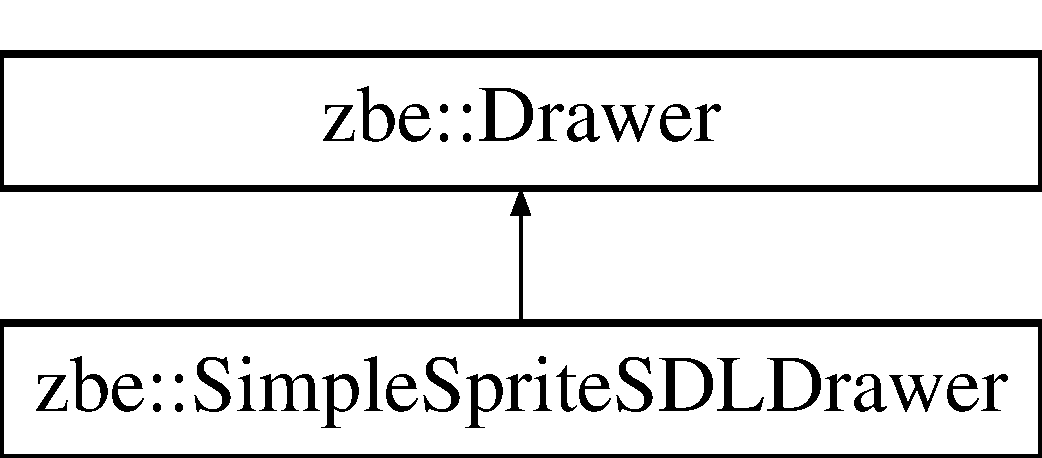
\includegraphics[height=2.000000cm]{classzbe_1_1_simple_sprite_s_d_l_drawer}
\end{center}
\end{figure}
\subsection*{Public Member Functions}
\begin{DoxyCompactItemize}
\item 
\hyperlink{classzbe_1_1_simple_sprite_s_d_l_drawer_a71a07190fa1d7a0c1aca3fe961c1b930}{Simple\+Sprite\+S\+D\+L\+Drawer} (\hyperlink{classzbe_1_1_window}{Window} $\ast$window, \hyperlink{namespacezbe_aa6d4affc7b95360c2d43d5fde9837a1f}{Simple\+Sprite\+Iterator} first, \hyperlink{namespacezbe_aa6d4affc7b95360c2d43d5fde9837a1f}{Simple\+Sprite\+Iterator} end)
\item 
\hyperlink{classzbe_1_1_simple_sprite_s_d_l_drawer_a8e2fd374fa5515e68355c1fbfe155bd8}{$\sim$\+Simple\+Sprite\+S\+D\+L\+Drawer} ()
\item 
void \hyperlink{classzbe_1_1_simple_sprite_s_d_l_drawer_af807a5376aafaa13dce5b8e8edf3973b}{draw} ()
\end{DoxyCompactItemize}


\subsection{Detailed Description}


Definition at line 36 of file Simple\+Sprite\+S\+D\+L\+Drawer.\+h.



\subsection{Constructor \& Destructor Documentation}
\hypertarget{classzbe_1_1_simple_sprite_s_d_l_drawer_a71a07190fa1d7a0c1aca3fe961c1b930}{}\index{zbe\+::\+Simple\+Sprite\+S\+D\+L\+Drawer@{zbe\+::\+Simple\+Sprite\+S\+D\+L\+Drawer}!Simple\+Sprite\+S\+D\+L\+Drawer@{Simple\+Sprite\+S\+D\+L\+Drawer}}
\index{Simple\+Sprite\+S\+D\+L\+Drawer@{Simple\+Sprite\+S\+D\+L\+Drawer}!zbe\+::\+Simple\+Sprite\+S\+D\+L\+Drawer@{zbe\+::\+Simple\+Sprite\+S\+D\+L\+Drawer}}
\subsubsection[{Simple\+Sprite\+S\+D\+L\+Drawer(\+Window $\ast$window, Simple\+Sprite\+Iterator first, Simple\+Sprite\+Iterator end)}]{\setlength{\rightskip}{0pt plus 5cm}zbe\+::\+Simple\+Sprite\+S\+D\+L\+Drawer\+::\+Simple\+Sprite\+S\+D\+L\+Drawer (
\begin{DoxyParamCaption}
\item[{{\bf Window} $\ast$}]{window, }
\item[{{\bf Simple\+Sprite\+Iterator}}]{first, }
\item[{{\bf Simple\+Sprite\+Iterator}}]{end}
\end{DoxyParamCaption}
)\hspace{0.3cm}{\ttfamily [inline]}}\label{classzbe_1_1_simple_sprite_s_d_l_drawer_a71a07190fa1d7a0c1aca3fe961c1b930}


Definition at line 38 of file Simple\+Sprite\+S\+D\+L\+Drawer.\+h.

\hypertarget{classzbe_1_1_simple_sprite_s_d_l_drawer_a8e2fd374fa5515e68355c1fbfe155bd8}{}\index{zbe\+::\+Simple\+Sprite\+S\+D\+L\+Drawer@{zbe\+::\+Simple\+Sprite\+S\+D\+L\+Drawer}!````~Simple\+Sprite\+S\+D\+L\+Drawer@{$\sim$\+Simple\+Sprite\+S\+D\+L\+Drawer}}
\index{````~Simple\+Sprite\+S\+D\+L\+Drawer@{$\sim$\+Simple\+Sprite\+S\+D\+L\+Drawer}!zbe\+::\+Simple\+Sprite\+S\+D\+L\+Drawer@{zbe\+::\+Simple\+Sprite\+S\+D\+L\+Drawer}}
\subsubsection[{$\sim$\+Simple\+Sprite\+S\+D\+L\+Drawer()}]{\setlength{\rightskip}{0pt plus 5cm}zbe\+::\+Simple\+Sprite\+S\+D\+L\+Drawer\+::$\sim$\+Simple\+Sprite\+S\+D\+L\+Drawer (
\begin{DoxyParamCaption}
{}
\end{DoxyParamCaption}
)\hspace{0.3cm}{\ttfamily [inline]}}\label{classzbe_1_1_simple_sprite_s_d_l_drawer_a8e2fd374fa5515e68355c1fbfe155bd8}


Definition at line 39 of file Simple\+Sprite\+S\+D\+L\+Drawer.\+h.



\subsection{Member Function Documentation}
\hypertarget{classzbe_1_1_simple_sprite_s_d_l_drawer_af807a5376aafaa13dce5b8e8edf3973b}{}\index{zbe\+::\+Simple\+Sprite\+S\+D\+L\+Drawer@{zbe\+::\+Simple\+Sprite\+S\+D\+L\+Drawer}!draw@{draw}}
\index{draw@{draw}!zbe\+::\+Simple\+Sprite\+S\+D\+L\+Drawer@{zbe\+::\+Simple\+Sprite\+S\+D\+L\+Drawer}}
\subsubsection[{draw()}]{\setlength{\rightskip}{0pt plus 5cm}void zbe\+::\+Simple\+Sprite\+S\+D\+L\+Drawer\+::draw (
\begin{DoxyParamCaption}
{}
\end{DoxyParamCaption}
)\hspace{0.3cm}{\ttfamily [virtual]}}\label{classzbe_1_1_simple_sprite_s_d_l_drawer_af807a5376aafaa13dce5b8e8edf3973b}


Implements \hyperlink{classzbe_1_1_drawer_ab890c0619125829ff83db906b1d1eb9d}{zbe\+::\+Drawer}.



The documentation for this class was generated from the following file\+:\begin{DoxyCompactItemize}
\item 
include/\+Z\+B\+E/core/drawers/\+S\+D\+L/\hyperlink{_simple_sprite_s_d_l_drawer_8h}{Simple\+Sprite\+S\+D\+L\+Drawer.\+h}\end{DoxyCompactItemize}

\hypertarget{structzbe_1_1_sphere}{}\section{zbe\+:\+:Sphere Struct Reference}
\label{structzbe_1_1_sphere}\index{zbe\+::\+Sphere@{zbe\+::\+Sphere}}


{\ttfamily \#include $<$objects.\+h$>$}

Inheritance diagram for zbe\+:\+:Sphere\+:\begin{figure}[H]
\begin{center}
\leavevmode
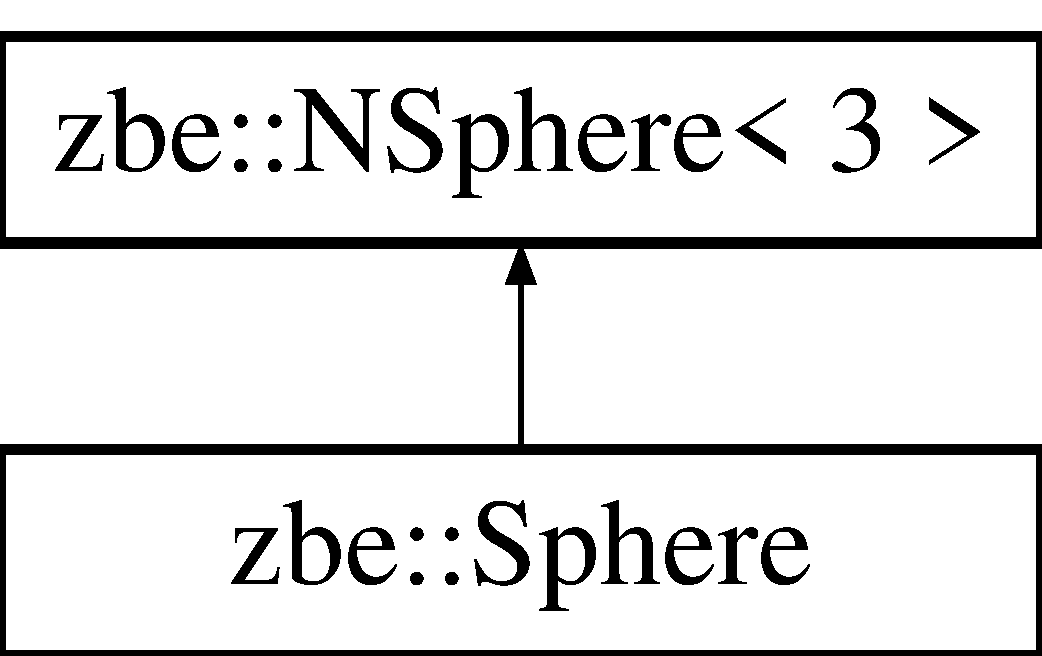
\includegraphics[height=2.000000cm]{structzbe_1_1_sphere}
\end{center}
\end{figure}
\subsection*{Public Member Functions}
\begin{DoxyCompactItemize}
\item 
\hyperlink{structzbe_1_1_sphere_a5ee555bba4b00aa2f9443798db6ad1b2}{Sphere} ()
\item 
\hyperlink{structzbe_1_1_sphere_afa2b11ef41dc5b17c94011d8863ffe09}{Sphere} (\hyperlink{classzbe_1_1_point}{Point}$<$ 3 $>$ center, double radius)
\item 
\hyperlink{structzbe_1_1_sphere_ac274ea3214a97d200cdd7c62c046dd91}{Sphere} (std\+::initializer\+\_\+list$<$ double $>$ lc, double \hyperlink{structzbe_1_1_n_sphere_ac8fae694bd80717eec61699b4d5206c6}{r})
\end{DoxyCompactItemize}
\subsection*{Additional Inherited Members}


\subsection{Detailed Description}


Definition at line 60 of file objects.\+h.



\subsection{Constructor \& Destructor Documentation}
\hypertarget{structzbe_1_1_sphere_a5ee555bba4b00aa2f9443798db6ad1b2}{}\index{zbe\+::\+Sphere@{zbe\+::\+Sphere}!Sphere@{Sphere}}
\index{Sphere@{Sphere}!zbe\+::\+Sphere@{zbe\+::\+Sphere}}
\subsubsection[{Sphere()}]{\setlength{\rightskip}{0pt plus 5cm}zbe\+::\+Sphere\+::\+Sphere (
\begin{DoxyParamCaption}
{}
\end{DoxyParamCaption}
)\hspace{0.3cm}{\ttfamily [inline]}}\label{structzbe_1_1_sphere_a5ee555bba4b00aa2f9443798db6ad1b2}


Definition at line 61 of file objects.\+h.

\hypertarget{structzbe_1_1_sphere_afa2b11ef41dc5b17c94011d8863ffe09}{}\index{zbe\+::\+Sphere@{zbe\+::\+Sphere}!Sphere@{Sphere}}
\index{Sphere@{Sphere}!zbe\+::\+Sphere@{zbe\+::\+Sphere}}
\subsubsection[{Sphere(\+Point$<$ 3 $>$ center, double radius)}]{\setlength{\rightskip}{0pt plus 5cm}zbe\+::\+Sphere\+::\+Sphere (
\begin{DoxyParamCaption}
\item[{{\bf Point}$<$ 3 $>$}]{center, }
\item[{double}]{radius}
\end{DoxyParamCaption}
)\hspace{0.3cm}{\ttfamily [inline]}}\label{structzbe_1_1_sphere_afa2b11ef41dc5b17c94011d8863ffe09}


Definition at line 62 of file objects.\+h.

\hypertarget{structzbe_1_1_sphere_ac274ea3214a97d200cdd7c62c046dd91}{}\index{zbe\+::\+Sphere@{zbe\+::\+Sphere}!Sphere@{Sphere}}
\index{Sphere@{Sphere}!zbe\+::\+Sphere@{zbe\+::\+Sphere}}
\subsubsection[{Sphere(std\+::initializer\+\_\+list$<$ double $>$ lc, double r)}]{\setlength{\rightskip}{0pt plus 5cm}zbe\+::\+Sphere\+::\+Sphere (
\begin{DoxyParamCaption}
\item[{std\+::initializer\+\_\+list$<$ double $>$}]{lc, }
\item[{double}]{r}
\end{DoxyParamCaption}
)\hspace{0.3cm}{\ttfamily [inline]}}\label{structzbe_1_1_sphere_ac274ea3214a97d200cdd7c62c046dd91}


Definition at line 63 of file objects.\+h.



The documentation for this struct was generated from the following file\+:\begin{DoxyCompactItemize}
\item 
include/\+Z\+B\+E/core/tools/math/\hyperlink{objects_8h}{objects.\+h}\end{DoxyCompactItemize}

\hypertarget{classzbe_1_1_sphere_collisionable}{}\section{zbe\+:\+:Sphere\+Collisionable Class Reference}
\label{classzbe_1_1_sphere_collisionable}\index{zbe\+::\+Sphere\+Collisionable@{zbe\+::\+Sphere\+Collisionable}}


{\ttfamily \#include $<$Sphere\+Collisionable.\+h$>$}

\subsection*{Public Member Functions}
\begin{DoxyCompactItemize}
\item 
\hyperlink{classzbe_1_1_sphere_collisionable_ac6104df39ed6b19643e336f01162f027}{Sphere\+Collisionable} ()
\item 
\hyperlink{classzbe_1_1_sphere_collisionable_a205d1c610acd836dc53b70902178a132}{Sphere\+Collisionable} (int x, int y, unsigned radius)
\item 
\hyperlink{classzbe_1_1_sphere_collisionable_acc7ff679ae8ffe1d597f9c621015c4cb}{$\sim$\+Sphere\+Collisionable} ()
\item 
void \hyperlink{classzbe_1_1_sphere_collisionable_ae4cb4df9c8406391dd36e7ca87fb0199}{set\+X} (int x)
\item 
void \hyperlink{classzbe_1_1_sphere_collisionable_add3a91da7f4d20e604a963570015189f}{set\+Y} (int y)
\item 
void \hyperlink{classzbe_1_1_sphere_collisionable_a1ba139746e5b18814d7b00cf0221b757}{set\+Radius} (unsigned radius)
\item 
int \hyperlink{classzbe_1_1_sphere_collisionable_a44e70ae23d8bb1dd6d27b7b329f700ac}{get\+X} () const 
\item 
int \hyperlink{classzbe_1_1_sphere_collisionable_a6e3fde0b9d686f49564cee9ef8aceef4}{get\+Y} () const 
\item 
unsigned \hyperlink{classzbe_1_1_sphere_collisionable_a5ed9a7f7a29ddf7175955da06b145c2c}{get\+Radius} () const 
\end{DoxyCompactItemize}


\subsection{Detailed Description}


Definition at line 15 of file Sphere\+Collisionable.\+h.



\subsection{Constructor \& Destructor Documentation}
\hypertarget{classzbe_1_1_sphere_collisionable_ac6104df39ed6b19643e336f01162f027}{}\index{zbe\+::\+Sphere\+Collisionable@{zbe\+::\+Sphere\+Collisionable}!Sphere\+Collisionable@{Sphere\+Collisionable}}
\index{Sphere\+Collisionable@{Sphere\+Collisionable}!zbe\+::\+Sphere\+Collisionable@{zbe\+::\+Sphere\+Collisionable}}
\subsubsection[{Sphere\+Collisionable()}]{\setlength{\rightskip}{0pt plus 5cm}zbe\+::\+Sphere\+Collisionable\+::\+Sphere\+Collisionable (
\begin{DoxyParamCaption}
{}
\end{DoxyParamCaption}
)\hspace{0.3cm}{\ttfamily [inline]}}\label{classzbe_1_1_sphere_collisionable_ac6104df39ed6b19643e336f01162f027}


Definition at line 17 of file Sphere\+Collisionable.\+h.

\hypertarget{classzbe_1_1_sphere_collisionable_a205d1c610acd836dc53b70902178a132}{}\index{zbe\+::\+Sphere\+Collisionable@{zbe\+::\+Sphere\+Collisionable}!Sphere\+Collisionable@{Sphere\+Collisionable}}
\index{Sphere\+Collisionable@{Sphere\+Collisionable}!zbe\+::\+Sphere\+Collisionable@{zbe\+::\+Sphere\+Collisionable}}
\subsubsection[{Sphere\+Collisionable(int x, int y, unsigned radius)}]{\setlength{\rightskip}{0pt plus 5cm}zbe\+::\+Sphere\+Collisionable\+::\+Sphere\+Collisionable (
\begin{DoxyParamCaption}
\item[{int}]{x, }
\item[{int}]{y, }
\item[{unsigned}]{radius}
\end{DoxyParamCaption}
)\hspace{0.3cm}{\ttfamily [inline]}}\label{classzbe_1_1_sphere_collisionable_a205d1c610acd836dc53b70902178a132}


Definition at line 18 of file Sphere\+Collisionable.\+h.

\hypertarget{classzbe_1_1_sphere_collisionable_acc7ff679ae8ffe1d597f9c621015c4cb}{}\index{zbe\+::\+Sphere\+Collisionable@{zbe\+::\+Sphere\+Collisionable}!````~Sphere\+Collisionable@{$\sim$\+Sphere\+Collisionable}}
\index{````~Sphere\+Collisionable@{$\sim$\+Sphere\+Collisionable}!zbe\+::\+Sphere\+Collisionable@{zbe\+::\+Sphere\+Collisionable}}
\subsubsection[{$\sim$\+Sphere\+Collisionable()}]{\setlength{\rightskip}{0pt plus 5cm}zbe\+::\+Sphere\+Collisionable\+::$\sim$\+Sphere\+Collisionable (
\begin{DoxyParamCaption}
{}
\end{DoxyParamCaption}
)\hspace{0.3cm}{\ttfamily [inline]}}\label{classzbe_1_1_sphere_collisionable_acc7ff679ae8ffe1d597f9c621015c4cb}


Definition at line 20 of file Sphere\+Collisionable.\+h.



\subsection{Member Function Documentation}
\hypertarget{classzbe_1_1_sphere_collisionable_a5ed9a7f7a29ddf7175955da06b145c2c}{}\index{zbe\+::\+Sphere\+Collisionable@{zbe\+::\+Sphere\+Collisionable}!get\+Radius@{get\+Radius}}
\index{get\+Radius@{get\+Radius}!zbe\+::\+Sphere\+Collisionable@{zbe\+::\+Sphere\+Collisionable}}
\subsubsection[{get\+Radius() const }]{\setlength{\rightskip}{0pt plus 5cm}unsigned zbe\+::\+Sphere\+Collisionable\+::get\+Radius (
\begin{DoxyParamCaption}
{}
\end{DoxyParamCaption}
) const\hspace{0.3cm}{\ttfamily [inline]}}\label{classzbe_1_1_sphere_collisionable_a5ed9a7f7a29ddf7175955da06b145c2c}


Definition at line 28 of file Sphere\+Collisionable.\+h.

\hypertarget{classzbe_1_1_sphere_collisionable_a44e70ae23d8bb1dd6d27b7b329f700ac}{}\index{zbe\+::\+Sphere\+Collisionable@{zbe\+::\+Sphere\+Collisionable}!get\+X@{get\+X}}
\index{get\+X@{get\+X}!zbe\+::\+Sphere\+Collisionable@{zbe\+::\+Sphere\+Collisionable}}
\subsubsection[{get\+X() const }]{\setlength{\rightskip}{0pt plus 5cm}int zbe\+::\+Sphere\+Collisionable\+::get\+X (
\begin{DoxyParamCaption}
{}
\end{DoxyParamCaption}
) const\hspace{0.3cm}{\ttfamily [inline]}}\label{classzbe_1_1_sphere_collisionable_a44e70ae23d8bb1dd6d27b7b329f700ac}


Definition at line 26 of file Sphere\+Collisionable.\+h.

\hypertarget{classzbe_1_1_sphere_collisionable_a6e3fde0b9d686f49564cee9ef8aceef4}{}\index{zbe\+::\+Sphere\+Collisionable@{zbe\+::\+Sphere\+Collisionable}!get\+Y@{get\+Y}}
\index{get\+Y@{get\+Y}!zbe\+::\+Sphere\+Collisionable@{zbe\+::\+Sphere\+Collisionable}}
\subsubsection[{get\+Y() const }]{\setlength{\rightskip}{0pt plus 5cm}int zbe\+::\+Sphere\+Collisionable\+::get\+Y (
\begin{DoxyParamCaption}
{}
\end{DoxyParamCaption}
) const\hspace{0.3cm}{\ttfamily [inline]}}\label{classzbe_1_1_sphere_collisionable_a6e3fde0b9d686f49564cee9ef8aceef4}


Definition at line 27 of file Sphere\+Collisionable.\+h.

\hypertarget{classzbe_1_1_sphere_collisionable_a1ba139746e5b18814d7b00cf0221b757}{}\index{zbe\+::\+Sphere\+Collisionable@{zbe\+::\+Sphere\+Collisionable}!set\+Radius@{set\+Radius}}
\index{set\+Radius@{set\+Radius}!zbe\+::\+Sphere\+Collisionable@{zbe\+::\+Sphere\+Collisionable}}
\subsubsection[{set\+Radius(unsigned radius)}]{\setlength{\rightskip}{0pt plus 5cm}void zbe\+::\+Sphere\+Collisionable\+::set\+Radius (
\begin{DoxyParamCaption}
\item[{unsigned}]{radius}
\end{DoxyParamCaption}
)\hspace{0.3cm}{\ttfamily [inline]}}\label{classzbe_1_1_sphere_collisionable_a1ba139746e5b18814d7b00cf0221b757}


Definition at line 24 of file Sphere\+Collisionable.\+h.

\hypertarget{classzbe_1_1_sphere_collisionable_ae4cb4df9c8406391dd36e7ca87fb0199}{}\index{zbe\+::\+Sphere\+Collisionable@{zbe\+::\+Sphere\+Collisionable}!set\+X@{set\+X}}
\index{set\+X@{set\+X}!zbe\+::\+Sphere\+Collisionable@{zbe\+::\+Sphere\+Collisionable}}
\subsubsection[{set\+X(int x)}]{\setlength{\rightskip}{0pt plus 5cm}void zbe\+::\+Sphere\+Collisionable\+::set\+X (
\begin{DoxyParamCaption}
\item[{int}]{x}
\end{DoxyParamCaption}
)\hspace{0.3cm}{\ttfamily [inline]}}\label{classzbe_1_1_sphere_collisionable_ae4cb4df9c8406391dd36e7ca87fb0199}


Definition at line 22 of file Sphere\+Collisionable.\+h.

\hypertarget{classzbe_1_1_sphere_collisionable_add3a91da7f4d20e604a963570015189f}{}\index{zbe\+::\+Sphere\+Collisionable@{zbe\+::\+Sphere\+Collisionable}!set\+Y@{set\+Y}}
\index{set\+Y@{set\+Y}!zbe\+::\+Sphere\+Collisionable@{zbe\+::\+Sphere\+Collisionable}}
\subsubsection[{set\+Y(int y)}]{\setlength{\rightskip}{0pt plus 5cm}void zbe\+::\+Sphere\+Collisionable\+::set\+Y (
\begin{DoxyParamCaption}
\item[{int}]{y}
\end{DoxyParamCaption}
)\hspace{0.3cm}{\ttfamily [inline]}}\label{classzbe_1_1_sphere_collisionable_add3a91da7f4d20e604a963570015189f}


Definition at line 23 of file Sphere\+Collisionable.\+h.



The documentation for this class was generated from the following file\+:\begin{DoxyCompactItemize}
\item 
include/\+Z\+B\+E/core/archetypes/\hyperlink{_sphere_collisionable_8h}{Sphere\+Collisionable.\+h}\end{DoxyCompactItemize}

\hypertarget{classzbe_1_1_sys_error}{}\section{zbe\+:\+:Sys\+Error Class Reference}
\label{classzbe_1_1_sys_error}\index{zbe\+::\+Sys\+Error@{zbe\+::\+Sys\+Error}}


A system class to inform about errors.  




{\ttfamily \#include $<$Sys\+Error.\+h$>$}

\subsection*{Static Public Member Functions}
\begin{DoxyCompactItemize}
\item 
static void \hyperlink{classzbe_1_1_sys_error_ac6ec5427abbbb641f5ad8dcd7f42e3fc}{set\+Error} (std\+::string error\+String)
\begin{DoxyCompactList}\small\item\em Set a new error. \end{DoxyCompactList}\item 
static int \hyperlink{classzbe_1_1_sys_error_a76f58259f20be485bbbb6c2ef3da9c61}{get\+N\+Errors} ()
\begin{DoxyCompactList}\small\item\em Return the number of calls to set\+Error. \end{DoxyCompactList}\item 
static std\+::string \hyperlink{classzbe_1_1_sys_error_ae37dcefda00e9c5251825d98df183ce9}{get\+First\+Error\+String} ()
\begin{DoxyCompactList}\small\item\em Return the error message of the first error. \end{DoxyCompactList}\item 
static void \hyperlink{classzbe_1_1_sys_error_aa402e67479e917839290230b47976c5b}{clear} ()
\begin{DoxyCompactList}\small\item\em Set error counter to 0 and empty the error string. \end{DoxyCompactList}\end{DoxyCompactItemize}


\subsection{Detailed Description}
A system class to inform about errors. 

Store the number of errors (calls to set\+Error) and the text for the first error. 

Definition at line 22 of file Sys\+Error.\+h.



\subsection{Member Function Documentation}
\hypertarget{classzbe_1_1_sys_error_aa402e67479e917839290230b47976c5b}{}\index{zbe\+::\+Sys\+Error@{zbe\+::\+Sys\+Error}!clear@{clear}}
\index{clear@{clear}!zbe\+::\+Sys\+Error@{zbe\+::\+Sys\+Error}}
\subsubsection[{clear()}]{\setlength{\rightskip}{0pt plus 5cm}static void zbe\+::\+Sys\+Error\+::clear (
\begin{DoxyParamCaption}
{}
\end{DoxyParamCaption}
)\hspace{0.3cm}{\ttfamily [static]}}\label{classzbe_1_1_sys_error_aa402e67479e917839290230b47976c5b}


Set error counter to 0 and empty the error string. 

\hypertarget{classzbe_1_1_sys_error_ae37dcefda00e9c5251825d98df183ce9}{}\index{zbe\+::\+Sys\+Error@{zbe\+::\+Sys\+Error}!get\+First\+Error\+String@{get\+First\+Error\+String}}
\index{get\+First\+Error\+String@{get\+First\+Error\+String}!zbe\+::\+Sys\+Error@{zbe\+::\+Sys\+Error}}
\subsubsection[{get\+First\+Error\+String()}]{\setlength{\rightskip}{0pt plus 5cm}static std\+::string zbe\+::\+Sys\+Error\+::get\+First\+Error\+String (
\begin{DoxyParamCaption}
{}
\end{DoxyParamCaption}
)\hspace{0.3cm}{\ttfamily [static]}}\label{classzbe_1_1_sys_error_ae37dcefda00e9c5251825d98df183ce9}


Return the error message of the first error. 

If there is, at least, one call to set\+Error, this function return the string message of the first error, empty string otherwise.

\begin{DoxyReturn}{Returns}
the first (if any) error string. 
\end{DoxyReturn}
\begin{DoxySeeAlso}{See also}
\hyperlink{classzbe_1_1_sys_error_ac6ec5427abbbb641f5ad8dcd7f42e3fc}{set\+Error()} and \hyperlink{classzbe_1_1_sys_error_aa402e67479e917839290230b47976c5b}{clear()} 
\end{DoxySeeAlso}
\hypertarget{classzbe_1_1_sys_error_a76f58259f20be485bbbb6c2ef3da9c61}{}\index{zbe\+::\+Sys\+Error@{zbe\+::\+Sys\+Error}!get\+N\+Errors@{get\+N\+Errors}}
\index{get\+N\+Errors@{get\+N\+Errors}!zbe\+::\+Sys\+Error@{zbe\+::\+Sys\+Error}}
\subsubsection[{get\+N\+Errors()}]{\setlength{\rightskip}{0pt plus 5cm}static int zbe\+::\+Sys\+Error\+::get\+N\+Errors (
\begin{DoxyParamCaption}
{}
\end{DoxyParamCaption}
)\hspace{0.3cm}{\ttfamily [static]}}\label{classzbe_1_1_sys_error_a76f58259f20be485bbbb6c2ef3da9c61}


Return the number of calls to set\+Error. 

\begin{DoxyReturn}{Returns}
the number of errors so far. 
\end{DoxyReturn}
\begin{DoxySeeAlso}{See also}
\hyperlink{classzbe_1_1_sys_error_ac6ec5427abbbb641f5ad8dcd7f42e3fc}{set\+Error()} and \hyperlink{classzbe_1_1_sys_error_aa402e67479e917839290230b47976c5b}{clear()} 
\end{DoxySeeAlso}
\hypertarget{classzbe_1_1_sys_error_ac6ec5427abbbb641f5ad8dcd7f42e3fc}{}\index{zbe\+::\+Sys\+Error@{zbe\+::\+Sys\+Error}!set\+Error@{set\+Error}}
\index{set\+Error@{set\+Error}!zbe\+::\+Sys\+Error@{zbe\+::\+Sys\+Error}}
\subsubsection[{set\+Error(std\+::string error\+String)}]{\setlength{\rightskip}{0pt plus 5cm}static void zbe\+::\+Sys\+Error\+::set\+Error (
\begin{DoxyParamCaption}
\item[{std\+::string}]{error\+String}
\end{DoxyParamCaption}
)\hspace{0.3cm}{\ttfamily [static]}}\label{classzbe_1_1_sys_error_ac6ec5427abbbb641f5ad8dcd7f42e3fc}


Set a new error. 

Increment the error counter in 1. If this is the first call, also stores the error\+String string.


\begin{DoxyParams}{Parameters}
{\em error\+String} & the description of the error \\
\hline
\end{DoxyParams}
\begin{DoxySeeAlso}{See also}
\hyperlink{classzbe_1_1_sys_error_a76f58259f20be485bbbb6c2ef3da9c61}{get\+N\+Errors()} and \hyperlink{classzbe_1_1_sys_error_ae37dcefda00e9c5251825d98df183ce9}{get\+First\+Error\+String()} 
\end{DoxySeeAlso}


The documentation for this class was generated from the following file\+:\begin{DoxyCompactItemize}
\item 
include/\+Z\+B\+E/core/system/\hyperlink{_sys_error_8h}{Sys\+Error.\+h}\end{DoxyCompactItemize}

\hypertarget{classzbe_1_1_ticket}{}\section{zbe\+:\+:Ticket Class Reference}
\label{classzbe_1_1_ticket}\index{zbe\+::\+Ticket@{zbe\+::\+Ticket}}


{\ttfamily \#include $<$Ticket.\+h$>$}

\subsection*{Public Types}
\begin{DoxyCompactItemize}
\item 
enum \hyperlink{classzbe_1_1_ticket_a8325e68db1e22dd969cc089bac3b1c3c}{State} \{ \hyperlink{classzbe_1_1_ticket_a8325e68db1e22dd969cc089bac3b1c3ca9a9c7fb95522615209a8db441eae9e53}{A\+C\+T\+I\+V\+E}, 
\hyperlink{classzbe_1_1_ticket_a8325e68db1e22dd969cc089bac3b1c3cafe4b1fdf81c91c449f0325de0ee46559}{I\+N\+A\+C\+T\+I\+V\+E}, 
\hyperlink{classzbe_1_1_ticket_a8325e68db1e22dd969cc089bac3b1c3caf97068955399e6f40421564c7c2f100f}{E\+R\+A\+S\+E\+D}
 \}
\end{DoxyCompactItemize}
\subsection*{Public Member Functions}
\begin{DoxyCompactItemize}
\item 
\hyperlink{classzbe_1_1_ticket_a54f4d3c170f63ee107ab6edc34c1c479}{Ticket} (\hyperlink{classzbe_1_1_ticket_a8325e68db1e22dd969cc089bac3b1c3c}{State} state=\hyperlink{classzbe_1_1_ticket_a8325e68db1e22dd969cc089bac3b1c3ca9a9c7fb95522615209a8db441eae9e53}{A\+C\+T\+I\+V\+E})
\item 
virtual \hyperlink{classzbe_1_1_ticket_af86d9ef8af586a7af4e6238f9e821eba}{$\sim$\+Ticket} ()
\item 
void \hyperlink{classzbe_1_1_ticket_a753f554fc268847f4ea468eba1ca3734}{set\+State} (\hyperlink{classzbe_1_1_ticket_a8325e68db1e22dd969cc089bac3b1c3c}{State} state)
\item 
\hyperlink{classzbe_1_1_ticket_a8325e68db1e22dd969cc089bac3b1c3c}{State} \hyperlink{classzbe_1_1_ticket_a2ecec85d07785fda1f67897487103efe}{get\+State} () const 
\item 
void \hyperlink{classzbe_1_1_ticket_ac27a6ce1050dbc48e15aed8fb2b64671}{set\+A\+C\+T\+I\+V\+E} ()
\item 
void \hyperlink{classzbe_1_1_ticket_a37002be23f9c6544e3c47002069cffd2}{set\+I\+N\+A\+C\+T\+I\+V\+E} ()
\item 
void \hyperlink{classzbe_1_1_ticket_ae36cc689edf4e7ee55df5133de3cb0b2}{set\+E\+R\+A\+S\+E\+D} ()
\item 
bool \hyperlink{classzbe_1_1_ticket_a5f7de9a861c79f17399b33eb619df537}{is\+A\+C\+T\+I\+V\+E} ()
\item 
bool \hyperlink{classzbe_1_1_ticket_a7cc36918cbabb0eede8e2b2789d914f9}{is\+Not\+A\+C\+T\+I\+V\+E} ()
\item 
bool \hyperlink{classzbe_1_1_ticket_afc202e4e6cbd889f162fd81ad1c0976a}{is\+I\+N\+A\+C\+T\+I\+V\+E} ()
\item 
bool \hyperlink{classzbe_1_1_ticket_a4992dd2f976a55943f35cfe11b903d9a}{is\+E\+R\+A\+S\+E\+D} ()
\end{DoxyCompactItemize}


\subsection{Detailed Description}


Definition at line 16 of file Ticket.\+h.



\subsection{Member Enumeration Documentation}
\hypertarget{classzbe_1_1_ticket_a8325e68db1e22dd969cc089bac3b1c3c}{}\index{zbe\+::\+Ticket@{zbe\+::\+Ticket}!State@{State}}
\index{State@{State}!zbe\+::\+Ticket@{zbe\+::\+Ticket}}
\subsubsection[{State}]{\setlength{\rightskip}{0pt plus 5cm}enum {\bf zbe\+::\+Ticket\+::\+State}}\label{classzbe_1_1_ticket_a8325e68db1e22dd969cc089bac3b1c3c}
\begin{Desc}
\item[Enumerator]\par
\begin{description}
\index{A\+C\+T\+I\+V\+E@{A\+C\+T\+I\+V\+E}!zbe\+::\+Ticket@{zbe\+::\+Ticket}}\index{zbe\+::\+Ticket@{zbe\+::\+Ticket}!A\+C\+T\+I\+V\+E@{A\+C\+T\+I\+V\+E}}\item[{\em 
\hypertarget{classzbe_1_1_ticket_a8325e68db1e22dd969cc089bac3b1c3ca9a9c7fb95522615209a8db441eae9e53}{}A\+C\+T\+I\+V\+E\label{classzbe_1_1_ticket_a8325e68db1e22dd969cc089bac3b1c3ca9a9c7fb95522615209a8db441eae9e53}
}]\index{I\+N\+A\+C\+T\+I\+V\+E@{I\+N\+A\+C\+T\+I\+V\+E}!zbe\+::\+Ticket@{zbe\+::\+Ticket}}\index{zbe\+::\+Ticket@{zbe\+::\+Ticket}!I\+N\+A\+C\+T\+I\+V\+E@{I\+N\+A\+C\+T\+I\+V\+E}}\item[{\em 
\hypertarget{classzbe_1_1_ticket_a8325e68db1e22dd969cc089bac3b1c3cafe4b1fdf81c91c449f0325de0ee46559}{}I\+N\+A\+C\+T\+I\+V\+E\label{classzbe_1_1_ticket_a8325e68db1e22dd969cc089bac3b1c3cafe4b1fdf81c91c449f0325de0ee46559}
}]\index{E\+R\+A\+S\+E\+D@{E\+R\+A\+S\+E\+D}!zbe\+::\+Ticket@{zbe\+::\+Ticket}}\index{zbe\+::\+Ticket@{zbe\+::\+Ticket}!E\+R\+A\+S\+E\+D@{E\+R\+A\+S\+E\+D}}\item[{\em 
\hypertarget{classzbe_1_1_ticket_a8325e68db1e22dd969cc089bac3b1c3caf97068955399e6f40421564c7c2f100f}{}E\+R\+A\+S\+E\+D\label{classzbe_1_1_ticket_a8325e68db1e22dd969cc089bac3b1c3caf97068955399e6f40421564c7c2f100f}
}]\end{description}
\end{Desc}


Definition at line 18 of file Ticket.\+h.



\subsection{Constructor \& Destructor Documentation}
\hypertarget{classzbe_1_1_ticket_a54f4d3c170f63ee107ab6edc34c1c479}{}\index{zbe\+::\+Ticket@{zbe\+::\+Ticket}!Ticket@{Ticket}}
\index{Ticket@{Ticket}!zbe\+::\+Ticket@{zbe\+::\+Ticket}}
\subsubsection[{Ticket(\+State state=\+A\+C\+T\+I\+V\+E)}]{\setlength{\rightskip}{0pt plus 5cm}zbe\+::\+Ticket\+::\+Ticket (
\begin{DoxyParamCaption}
\item[{{\bf State}}]{state = {\ttfamily {\bf A\+C\+T\+I\+V\+E}}}
\end{DoxyParamCaption}
)\hspace{0.3cm}{\ttfamily [inline]}}\label{classzbe_1_1_ticket_a54f4d3c170f63ee107ab6edc34c1c479}


Definition at line 20 of file Ticket.\+h.

\hypertarget{classzbe_1_1_ticket_af86d9ef8af586a7af4e6238f9e821eba}{}\index{zbe\+::\+Ticket@{zbe\+::\+Ticket}!````~Ticket@{$\sim$\+Ticket}}
\index{````~Ticket@{$\sim$\+Ticket}!zbe\+::\+Ticket@{zbe\+::\+Ticket}}
\subsubsection[{$\sim$\+Ticket()}]{\setlength{\rightskip}{0pt plus 5cm}virtual zbe\+::\+Ticket\+::$\sim$\+Ticket (
\begin{DoxyParamCaption}
{}
\end{DoxyParamCaption}
)\hspace{0.3cm}{\ttfamily [inline]}, {\ttfamily [virtual]}}\label{classzbe_1_1_ticket_af86d9ef8af586a7af4e6238f9e821eba}


Definition at line 21 of file Ticket.\+h.



\subsection{Member Function Documentation}
\hypertarget{classzbe_1_1_ticket_a2ecec85d07785fda1f67897487103efe}{}\index{zbe\+::\+Ticket@{zbe\+::\+Ticket}!get\+State@{get\+State}}
\index{get\+State@{get\+State}!zbe\+::\+Ticket@{zbe\+::\+Ticket}}
\subsubsection[{get\+State() const }]{\setlength{\rightskip}{0pt plus 5cm}{\bf State} zbe\+::\+Ticket\+::get\+State (
\begin{DoxyParamCaption}
{}
\end{DoxyParamCaption}
) const\hspace{0.3cm}{\ttfamily [inline]}}\label{classzbe_1_1_ticket_a2ecec85d07785fda1f67897487103efe}


Definition at line 24 of file Ticket.\+h.

\hypertarget{classzbe_1_1_ticket_a5f7de9a861c79f17399b33eb619df537}{}\index{zbe\+::\+Ticket@{zbe\+::\+Ticket}!is\+A\+C\+T\+I\+V\+E@{is\+A\+C\+T\+I\+V\+E}}
\index{is\+A\+C\+T\+I\+V\+E@{is\+A\+C\+T\+I\+V\+E}!zbe\+::\+Ticket@{zbe\+::\+Ticket}}
\subsubsection[{is\+A\+C\+T\+I\+V\+E()}]{\setlength{\rightskip}{0pt plus 5cm}bool zbe\+::\+Ticket\+::is\+A\+C\+T\+I\+V\+E (
\begin{DoxyParamCaption}
{}
\end{DoxyParamCaption}
)\hspace{0.3cm}{\ttfamily [inline]}}\label{classzbe_1_1_ticket_a5f7de9a861c79f17399b33eb619df537}


Definition at line 30 of file Ticket.\+h.

\hypertarget{classzbe_1_1_ticket_a4992dd2f976a55943f35cfe11b903d9a}{}\index{zbe\+::\+Ticket@{zbe\+::\+Ticket}!is\+E\+R\+A\+S\+E\+D@{is\+E\+R\+A\+S\+E\+D}}
\index{is\+E\+R\+A\+S\+E\+D@{is\+E\+R\+A\+S\+E\+D}!zbe\+::\+Ticket@{zbe\+::\+Ticket}}
\subsubsection[{is\+E\+R\+A\+S\+E\+D()}]{\setlength{\rightskip}{0pt plus 5cm}bool zbe\+::\+Ticket\+::is\+E\+R\+A\+S\+E\+D (
\begin{DoxyParamCaption}
{}
\end{DoxyParamCaption}
)\hspace{0.3cm}{\ttfamily [inline]}}\label{classzbe_1_1_ticket_a4992dd2f976a55943f35cfe11b903d9a}


Definition at line 33 of file Ticket.\+h.

\hypertarget{classzbe_1_1_ticket_afc202e4e6cbd889f162fd81ad1c0976a}{}\index{zbe\+::\+Ticket@{zbe\+::\+Ticket}!is\+I\+N\+A\+C\+T\+I\+V\+E@{is\+I\+N\+A\+C\+T\+I\+V\+E}}
\index{is\+I\+N\+A\+C\+T\+I\+V\+E@{is\+I\+N\+A\+C\+T\+I\+V\+E}!zbe\+::\+Ticket@{zbe\+::\+Ticket}}
\subsubsection[{is\+I\+N\+A\+C\+T\+I\+V\+E()}]{\setlength{\rightskip}{0pt plus 5cm}bool zbe\+::\+Ticket\+::is\+I\+N\+A\+C\+T\+I\+V\+E (
\begin{DoxyParamCaption}
{}
\end{DoxyParamCaption}
)\hspace{0.3cm}{\ttfamily [inline]}}\label{classzbe_1_1_ticket_afc202e4e6cbd889f162fd81ad1c0976a}


Definition at line 32 of file Ticket.\+h.

\hypertarget{classzbe_1_1_ticket_a7cc36918cbabb0eede8e2b2789d914f9}{}\index{zbe\+::\+Ticket@{zbe\+::\+Ticket}!is\+Not\+A\+C\+T\+I\+V\+E@{is\+Not\+A\+C\+T\+I\+V\+E}}
\index{is\+Not\+A\+C\+T\+I\+V\+E@{is\+Not\+A\+C\+T\+I\+V\+E}!zbe\+::\+Ticket@{zbe\+::\+Ticket}}
\subsubsection[{is\+Not\+A\+C\+T\+I\+V\+E()}]{\setlength{\rightskip}{0pt plus 5cm}bool zbe\+::\+Ticket\+::is\+Not\+A\+C\+T\+I\+V\+E (
\begin{DoxyParamCaption}
{}
\end{DoxyParamCaption}
)\hspace{0.3cm}{\ttfamily [inline]}}\label{classzbe_1_1_ticket_a7cc36918cbabb0eede8e2b2789d914f9}


Definition at line 31 of file Ticket.\+h.

\hypertarget{classzbe_1_1_ticket_ac27a6ce1050dbc48e15aed8fb2b64671}{}\index{zbe\+::\+Ticket@{zbe\+::\+Ticket}!set\+A\+C\+T\+I\+V\+E@{set\+A\+C\+T\+I\+V\+E}}
\index{set\+A\+C\+T\+I\+V\+E@{set\+A\+C\+T\+I\+V\+E}!zbe\+::\+Ticket@{zbe\+::\+Ticket}}
\subsubsection[{set\+A\+C\+T\+I\+V\+E()}]{\setlength{\rightskip}{0pt plus 5cm}void zbe\+::\+Ticket\+::set\+A\+C\+T\+I\+V\+E (
\begin{DoxyParamCaption}
{}
\end{DoxyParamCaption}
)\hspace{0.3cm}{\ttfamily [inline]}}\label{classzbe_1_1_ticket_ac27a6ce1050dbc48e15aed8fb2b64671}


Definition at line 26 of file Ticket.\+h.

\hypertarget{classzbe_1_1_ticket_ae36cc689edf4e7ee55df5133de3cb0b2}{}\index{zbe\+::\+Ticket@{zbe\+::\+Ticket}!set\+E\+R\+A\+S\+E\+D@{set\+E\+R\+A\+S\+E\+D}}
\index{set\+E\+R\+A\+S\+E\+D@{set\+E\+R\+A\+S\+E\+D}!zbe\+::\+Ticket@{zbe\+::\+Ticket}}
\subsubsection[{set\+E\+R\+A\+S\+E\+D()}]{\setlength{\rightskip}{0pt plus 5cm}void zbe\+::\+Ticket\+::set\+E\+R\+A\+S\+E\+D (
\begin{DoxyParamCaption}
{}
\end{DoxyParamCaption}
)\hspace{0.3cm}{\ttfamily [inline]}}\label{classzbe_1_1_ticket_ae36cc689edf4e7ee55df5133de3cb0b2}


Definition at line 28 of file Ticket.\+h.

\hypertarget{classzbe_1_1_ticket_a37002be23f9c6544e3c47002069cffd2}{}\index{zbe\+::\+Ticket@{zbe\+::\+Ticket}!set\+I\+N\+A\+C\+T\+I\+V\+E@{set\+I\+N\+A\+C\+T\+I\+V\+E}}
\index{set\+I\+N\+A\+C\+T\+I\+V\+E@{set\+I\+N\+A\+C\+T\+I\+V\+E}!zbe\+::\+Ticket@{zbe\+::\+Ticket}}
\subsubsection[{set\+I\+N\+A\+C\+T\+I\+V\+E()}]{\setlength{\rightskip}{0pt plus 5cm}void zbe\+::\+Ticket\+::set\+I\+N\+A\+C\+T\+I\+V\+E (
\begin{DoxyParamCaption}
{}
\end{DoxyParamCaption}
)\hspace{0.3cm}{\ttfamily [inline]}}\label{classzbe_1_1_ticket_a37002be23f9c6544e3c47002069cffd2}


Definition at line 27 of file Ticket.\+h.

\hypertarget{classzbe_1_1_ticket_a753f554fc268847f4ea468eba1ca3734}{}\index{zbe\+::\+Ticket@{zbe\+::\+Ticket}!set\+State@{set\+State}}
\index{set\+State@{set\+State}!zbe\+::\+Ticket@{zbe\+::\+Ticket}}
\subsubsection[{set\+State(\+State state)}]{\setlength{\rightskip}{0pt plus 5cm}void zbe\+::\+Ticket\+::set\+State (
\begin{DoxyParamCaption}
\item[{{\bf State}}]{state}
\end{DoxyParamCaption}
)\hspace{0.3cm}{\ttfamily [inline]}}\label{classzbe_1_1_ticket_a753f554fc268847f4ea468eba1ca3734}


Definition at line 23 of file Ticket.\+h.



The documentation for this class was generated from the following file\+:\begin{DoxyCompactItemize}
\item 
include/\+Z\+B\+E/core/tools/containers/\hyperlink{_ticket_8h}{Ticket.\+h}\end{DoxyCompactItemize}

\hypertarget{classzbe_1_1_timer}{}\section{zbe\+:\+:Timer Class Reference}
\label{classzbe_1_1_timer}\index{zbe\+::\+Timer@{zbe\+::\+Timer}}


An abstract class to inform about time.  




{\ttfamily \#include $<$Timer.\+h$>$}

\subsection*{Public Member Functions}
\begin{DoxyCompactItemize}
\item 
virtual \hyperlink{classzbe_1_1_timer_a0580e55b28f6dde20240059de12dc1d8}{$\sim$\+Timer} ()
\begin{DoxyCompactList}\small\item\em Virtual destructor for inheritance. \end{DoxyCompactList}\item 
virtual void \hyperlink{classzbe_1_1_timer_a7ce01b37528ade45ab0fd31edfd5be71}{restart} ()=0
\begin{DoxyCompactList}\small\item\em Set the \hyperlink{classzbe_1_1_timer}{Timer} to zero. \end{DoxyCompactList}\item 
virtual void \hyperlink{classzbe_1_1_timer_acaee85b31f4055d1b704f9f033aba06a}{pause} ()=0
\begin{DoxyCompactList}\small\item\em Pause the \hyperlink{classzbe_1_1_timer}{Timer}, stop counting. \end{DoxyCompactList}\item 
virtual void \hyperlink{classzbe_1_1_timer_ae75a4ff2f543df264a8de58b246a9661}{resume} ()=0
\begin{DoxyCompactList}\small\item\em Resume the \hyperlink{classzbe_1_1_timer}{Timer}, continue the counting. \end{DoxyCompactList}\item 
virtual unsigned int \hyperlink{classzbe_1_1_timer_aac4d92010632f3b52253835eed9180eb}{get\+Milliseconds} ()=0
\begin{DoxyCompactList}\small\item\em Get the elapsed time in milliseconds. \end{DoxyCompactList}\end{DoxyCompactItemize}


\subsection{Detailed Description}
An abstract class to inform about time. 

Declare the basic functions of every \hyperlink{classzbe_1_1_timer}{Timer}. 

Definition at line 19 of file Timer.\+h.



\subsection{Constructor \& Destructor Documentation}
\hypertarget{classzbe_1_1_timer_a0580e55b28f6dde20240059de12dc1d8}{}\index{zbe\+::\+Timer@{zbe\+::\+Timer}!````~Timer@{$\sim$\+Timer}}
\index{````~Timer@{$\sim$\+Timer}!zbe\+::\+Timer@{zbe\+::\+Timer}}
\subsubsection[{$\sim$\+Timer()}]{\setlength{\rightskip}{0pt plus 5cm}virtual zbe\+::\+Timer\+::$\sim$\+Timer (
\begin{DoxyParamCaption}
{}
\end{DoxyParamCaption}
)\hspace{0.3cm}{\ttfamily [inline]}, {\ttfamily [virtual]}}\label{classzbe_1_1_timer_a0580e55b28f6dde20240059de12dc1d8}


Virtual destructor for inheritance. 



Definition at line 21 of file Timer.\+h.



\subsection{Member Function Documentation}
\hypertarget{classzbe_1_1_timer_aac4d92010632f3b52253835eed9180eb}{}\index{zbe\+::\+Timer@{zbe\+::\+Timer}!get\+Milliseconds@{get\+Milliseconds}}
\index{get\+Milliseconds@{get\+Milliseconds}!zbe\+::\+Timer@{zbe\+::\+Timer}}
\subsubsection[{get\+Milliseconds()=0}]{\setlength{\rightskip}{0pt plus 5cm}virtual unsigned int zbe\+::\+Timer\+::get\+Milliseconds (
\begin{DoxyParamCaption}
{}
\end{DoxyParamCaption}
)\hspace{0.3cm}{\ttfamily [pure virtual]}}\label{classzbe_1_1_timer_aac4d92010632f3b52253835eed9180eb}


Get the elapsed time in milliseconds. 

\hypertarget{classzbe_1_1_timer_acaee85b31f4055d1b704f9f033aba06a}{}\index{zbe\+::\+Timer@{zbe\+::\+Timer}!pause@{pause}}
\index{pause@{pause}!zbe\+::\+Timer@{zbe\+::\+Timer}}
\subsubsection[{pause()=0}]{\setlength{\rightskip}{0pt plus 5cm}virtual void zbe\+::\+Timer\+::pause (
\begin{DoxyParamCaption}
{}
\end{DoxyParamCaption}
)\hspace{0.3cm}{\ttfamily [pure virtual]}}\label{classzbe_1_1_timer_acaee85b31f4055d1b704f9f033aba06a}


Pause the \hyperlink{classzbe_1_1_timer}{Timer}, stop counting. 

\hypertarget{classzbe_1_1_timer_a7ce01b37528ade45ab0fd31edfd5be71}{}\index{zbe\+::\+Timer@{zbe\+::\+Timer}!restart@{restart}}
\index{restart@{restart}!zbe\+::\+Timer@{zbe\+::\+Timer}}
\subsubsection[{restart()=0}]{\setlength{\rightskip}{0pt plus 5cm}virtual void zbe\+::\+Timer\+::restart (
\begin{DoxyParamCaption}
{}
\end{DoxyParamCaption}
)\hspace{0.3cm}{\ttfamily [pure virtual]}}\label{classzbe_1_1_timer_a7ce01b37528ade45ab0fd31edfd5be71}


Set the \hyperlink{classzbe_1_1_timer}{Timer} to zero. 

\hypertarget{classzbe_1_1_timer_ae75a4ff2f543df264a8de58b246a9661}{}\index{zbe\+::\+Timer@{zbe\+::\+Timer}!resume@{resume}}
\index{resume@{resume}!zbe\+::\+Timer@{zbe\+::\+Timer}}
\subsubsection[{resume()=0}]{\setlength{\rightskip}{0pt plus 5cm}virtual void zbe\+::\+Timer\+::resume (
\begin{DoxyParamCaption}
{}
\end{DoxyParamCaption}
)\hspace{0.3cm}{\ttfamily [pure virtual]}}\label{classzbe_1_1_timer_ae75a4ff2f543df264a8de58b246a9661}


Resume the \hyperlink{classzbe_1_1_timer}{Timer}, continue the counting. 



The documentation for this class was generated from the following file\+:\begin{DoxyCompactItemize}
\item 
include/\+Z\+B\+E/core/tools/\hyperlink{_timer_8h}{Timer.\+h}\end{DoxyCompactItemize}

\hypertarget{classzbe_1_1_uniform_linear_motion}{}\section{zbe\+:\+:Uniform\+Linear\+Motion$<$ s $>$ Class Template Reference}
\label{classzbe_1_1_uniform_linear_motion}\index{zbe\+::\+Uniform\+Linear\+Motion$<$ s $>$@{zbe\+::\+Uniform\+Linear\+Motion$<$ s $>$}}


{\ttfamily \#include $<$Uniform\+Linear\+Motion.\+h$>$}

Inheritance diagram for zbe\+:\+:Uniform\+Linear\+Motion$<$ s $>$\+:\begin{figure}[H]
\begin{center}
\leavevmode
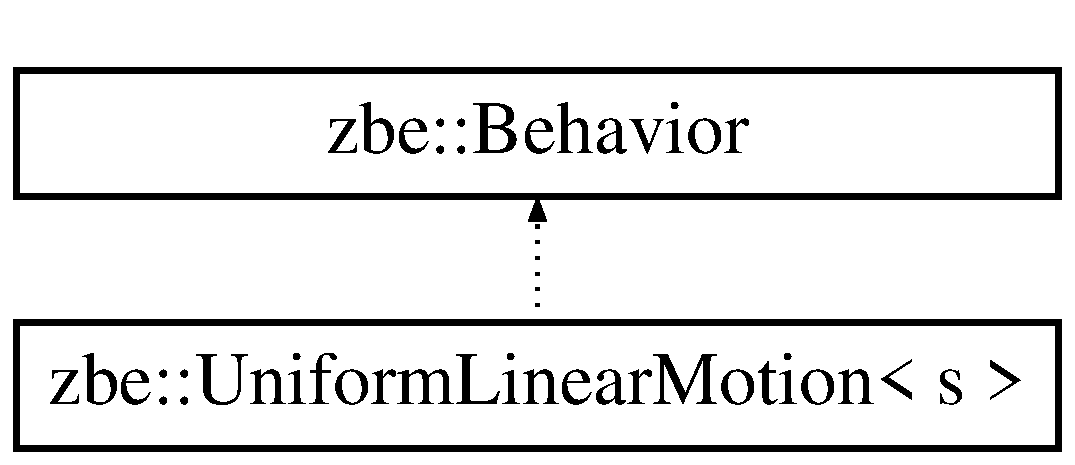
\includegraphics[height=2.000000cm]{classzbe_1_1_uniform_linear_motion}
\end{center}
\end{figure}
\subsection*{Public Member Functions}
\begin{DoxyCompactItemize}
\item 
\hyperlink{classzbe_1_1_uniform_linear_motion_a29ff82f8b26055cabe5fec9f8af02186}{$\sim$\+Uniform\+Linear\+Motion} ()
\item 
void \hyperlink{classzbe_1_1_uniform_linear_motion_a42678dd6e10f13645574f5e41611de82}{behave\+Until} (double time)
\end{DoxyCompactItemize}


\subsection{Detailed Description}
\subsubsection*{template$<$unsigned s$>$class zbe\+::\+Uniform\+Linear\+Motion$<$ s $>$}



Definition at line 38 of file Uniform\+Linear\+Motion.\+h.



\subsection{Constructor \& Destructor Documentation}
\hypertarget{classzbe_1_1_uniform_linear_motion_a29ff82f8b26055cabe5fec9f8af02186}{}\index{zbe\+::\+Uniform\+Linear\+Motion@{zbe\+::\+Uniform\+Linear\+Motion}!````~Uniform\+Linear\+Motion@{$\sim$\+Uniform\+Linear\+Motion}}
\index{````~Uniform\+Linear\+Motion@{$\sim$\+Uniform\+Linear\+Motion}!zbe\+::\+Uniform\+Linear\+Motion@{zbe\+::\+Uniform\+Linear\+Motion}}
\subsubsection[{$\sim$\+Uniform\+Linear\+Motion()}]{\setlength{\rightskip}{0pt plus 5cm}template$<$unsigned s$>$ {\bf zbe\+::\+Uniform\+Linear\+Motion}$<$ s $>$\+::$\sim${\bf Uniform\+Linear\+Motion} (
\begin{DoxyParamCaption}
{}
\end{DoxyParamCaption}
)\hspace{0.3cm}{\ttfamily [inline]}}\label{classzbe_1_1_uniform_linear_motion_a29ff82f8b26055cabe5fec9f8af02186}


Definition at line 40 of file Uniform\+Linear\+Motion.\+h.



\subsection{Member Function Documentation}
\hypertarget{classzbe_1_1_uniform_linear_motion_a42678dd6e10f13645574f5e41611de82}{}\index{zbe\+::\+Uniform\+Linear\+Motion@{zbe\+::\+Uniform\+Linear\+Motion}!behave\+Until@{behave\+Until}}
\index{behave\+Until@{behave\+Until}!zbe\+::\+Uniform\+Linear\+Motion@{zbe\+::\+Uniform\+Linear\+Motion}}
\subsubsection[{behave\+Until(double time)}]{\setlength{\rightskip}{0pt plus 5cm}template$<$unsigned s$>$ void {\bf zbe\+::\+Uniform\+Linear\+Motion}$<$ s $>$\+::behave\+Until (
\begin{DoxyParamCaption}
\item[{double}]{time}
\end{DoxyParamCaption}
)\hspace{0.3cm}{\ttfamily [virtual]}}\label{classzbe_1_1_uniform_linear_motion_a42678dd6e10f13645574f5e41611de82}


Implements \hyperlink{classzbe_1_1_behavior_a9bd7af2d6f39aafb11052e2ebdca3a71}{zbe\+::\+Behavior}.



The documentation for this class was generated from the following file\+:\begin{DoxyCompactItemize}
\item 
include/\+Z\+B\+E/core/behaviors/\hyperlink{_uniform_linear_motion_8h}{Uniform\+Linear\+Motion.\+h}\end{DoxyCompactItemize}

\hypertarget{classzbe_1_1_vector}{}\section{zbe\+:\+:Vector$<$ s $>$ Class Template Reference}
\label{classzbe_1_1_vector}\index{zbe\+::\+Vector$<$ s $>$@{zbe\+::\+Vector$<$ s $>$}}


A class that represent Vectors of any dimension.  




{\ttfamily \#include $<$Point.\+h$>$}

\subsection*{Public Member Functions}
\begin{DoxyCompactItemize}
\item 
\hyperlink{classzbe_1_1_vector_af478126eacae828b0d6454c5ae686c5f}{Vector} ()
\begin{DoxyCompactList}\small\item\em Void constructor, the \hyperlink{classzbe_1_1_vector}{Vector}\textquotesingle{}s values are unknown. \end{DoxyCompactList}\item 
\hyperlink{classzbe_1_1_vector_a7caf8410ba2f9f2d5671d4a1f1e5153c}{Vector} (std\+::initializer\+\_\+list$<$ double $>$ l)
\begin{DoxyCompactList}\small\item\em A list initializer constructor. \end{DoxyCompactList}\item 
double \& \hyperlink{classzbe_1_1_vector_a84bb0163dbc21094e70bf7340f4bb7dc}{operator\mbox{[}$\,$\mbox{]}} (std\+::size\+\_\+t idx)
\begin{DoxyCompactList}\small\item\em Implements direct access to \hyperlink{classzbe_1_1_vector}{Vector} values with operator\mbox{[}\mbox{]}. \end{DoxyCompactList}\item 
const double \& \hyperlink{classzbe_1_1_vector_a13087f897b6386630adf82f540fda49d}{operator\mbox{[}$\,$\mbox{]}} (std\+::size\+\_\+t idx) const 
\begin{DoxyCompactList}\small\item\em Implements direct access to \hyperlink{classzbe_1_1_vector}{Vector} values with operator\mbox{[}\mbox{]}. \end{DoxyCompactList}\item 
\hyperlink{classzbe_1_1_vector}{Vector}$<$ s $>$ \& \hyperlink{classzbe_1_1_vector_ae506e73798e78b596dd43be34bfbdd73}{operator+=} (\hyperlink{classzbe_1_1_vector}{Vector}$<$ s $>$ rhs)
\begin{DoxyCompactList}\small\item\em Implements \hyperlink{classzbe_1_1_vector}{Vector} addition. \end{DoxyCompactList}\item 
\hyperlink{classzbe_1_1_vector}{Vector}$<$ s $>$ \& \hyperlink{classzbe_1_1_vector_a879b33b5c6c62bc16b771cc874614189}{operator-\/=} (\hyperlink{classzbe_1_1_vector}{Vector}$<$ s $>$ rhs)
\begin{DoxyCompactList}\small\item\em Implements \hyperlink{classzbe_1_1_vector}{Vector} subtraction. \end{DoxyCompactList}\item 
\hyperlink{classzbe_1_1_vector}{Vector}$<$ s $>$ \& \hyperlink{classzbe_1_1_vector_a215c195ff041f6e8230c5ce619174651}{operator-\/} ()
\begin{DoxyCompactList}\small\item\em Changes the orientation of a vector changing the sign of its dimensions. \end{DoxyCompactList}\item 
\hyperlink{classzbe_1_1_vector}{Vector}$<$ s $>$ \& \hyperlink{classzbe_1_1_vector_a7088f4ab907e75ce8ba529189917c5ca}{operator$\ast$=} (double rhs)
\begin{DoxyCompactList}\small\item\em Implements \hyperlink{classzbe_1_1_vector}{Vector} multiplication by a scalar. \end{DoxyCompactList}\item 
double \hyperlink{classzbe_1_1_vector_aaff6572fe9c7ccb0ede8d017a135f4c1}{get\+Module} ()
\begin{DoxyCompactList}\small\item\em Compute the \hyperlink{classzbe_1_1_vector}{Vector} Module. \end{DoxyCompactList}\item 
double \hyperlink{classzbe_1_1_vector_ad9f7babae7c512392583c36d9611140b}{get\+Sqr\+Module} ()
\begin{DoxyCompactList}\small\item\em Compute the squared \hyperlink{classzbe_1_1_vector}{Vector} Module. \end{DoxyCompactList}\end{DoxyCompactItemize}
\subsection*{Protected Attributes}
\begin{DoxyCompactItemize}
\item 
double \hyperlink{classzbe_1_1_vector_a1adaf8d4244fe2c1d762d6c58f4b01eb}{data} \mbox{[}s\mbox{]}
\begin{DoxyCompactList}\small\item\em \hyperlink{classzbe_1_1_point}{Point} data. \end{DoxyCompactList}\end{DoxyCompactItemize}
\subsection*{Friends}
\begin{DoxyCompactItemize}
\item 
\hyperlink{classzbe_1_1_vector}{Vector} \hyperlink{classzbe_1_1_vector_aa00684a017bf5c29d04889cd160208dc}{operator+} (\hyperlink{classzbe_1_1_vector}{Vector} lhs, const \hyperlink{classzbe_1_1_vector}{Vector} \&rhs)
\begin{DoxyCompactList}\small\item\em Implements \hyperlink{classzbe_1_1_vector}{Vector} addition. \end{DoxyCompactList}\item 
\hyperlink{classzbe_1_1_vector}{Vector} \hyperlink{classzbe_1_1_vector_a4cc289b80e2fcb276841865d247a68e2}{operator+} (\hyperlink{classzbe_1_1_vector}{Vector} \&lhs, \hyperlink{classzbe_1_1_vector}{Vector} \&\&rhs)
\begin{DoxyCompactList}\small\item\em Implements \hyperlink{classzbe_1_1_vector}{Vector} addition. \end{DoxyCompactList}\item 
\hyperlink{classzbe_1_1_vector}{Vector} \hyperlink{classzbe_1_1_vector_a23f5fd27917e1626fc0a07fd5b635f66}{operator-\/} (\hyperlink{classzbe_1_1_vector}{Vector} lhs, const \hyperlink{classzbe_1_1_vector}{Vector} \&rhs)
\begin{DoxyCompactList}\small\item\em Implements \hyperlink{classzbe_1_1_vector}{Vector} subtraction. \end{DoxyCompactList}\item 
\hyperlink{classzbe_1_1_vector}{Vector} \hyperlink{classzbe_1_1_vector_a7a4ea7ee2d59cb2320f59d5ee8ed8b3c}{operator-\/} (const \hyperlink{classzbe_1_1_vector}{Vector} \&lhs, \hyperlink{classzbe_1_1_vector}{Vector} \&\&rhs)
\begin{DoxyCompactList}\small\item\em Implements \hyperlink{classzbe_1_1_vector}{Vector} subtraction. \end{DoxyCompactList}\item 
\hyperlink{classzbe_1_1_vector}{Vector} \hyperlink{classzbe_1_1_vector_ad2d25cf5fc77db8c11d242bd491b64f9}{operator$\ast$} (\hyperlink{classzbe_1_1_vector}{Vector} lhs, double rhs)
\begin{DoxyCompactList}\small\item\em Changes the orientation of a vector changing the sign of its dimensions. \end{DoxyCompactList}\item 
double \hyperlink{classzbe_1_1_vector_a0e8b1be97267a83a75eda5e387aeb635}{operator$\ast$} (const \hyperlink{classzbe_1_1_vector}{Vector} \&lhs, const \hyperlink{classzbe_1_1_vector}{Vector} \&rhs)
\begin{DoxyCompactList}\small\item\em Implements \hyperlink{classzbe_1_1_vector}{Vector} multiplication by a scalar. \end{DoxyCompactList}\end{DoxyCompactItemize}


\subsection{Detailed Description}
\subsubsection*{template$<$unsigned s$>$class zbe\+::\+Vector$<$ s $>$}

A class that represent Vectors of any dimension. 

This template needs to know the number of dimensions of the \hyperlink{classzbe_1_1_vector}{Vector}. 

Definition at line 20 of file Point.\+h.



\subsection{Constructor \& Destructor Documentation}
\hypertarget{classzbe_1_1_vector_af478126eacae828b0d6454c5ae686c5f}{}\index{zbe\+::\+Vector@{zbe\+::\+Vector}!Vector@{Vector}}
\index{Vector@{Vector}!zbe\+::\+Vector@{zbe\+::\+Vector}}
\subsubsection[{Vector()}]{\setlength{\rightskip}{0pt plus 5cm}template$<$unsigned s$>$ {\bf zbe\+::\+Vector}$<$ s $>$\+::{\bf Vector} (
\begin{DoxyParamCaption}
{}
\end{DoxyParamCaption}
)\hspace{0.3cm}{\ttfamily [inline]}}\label{classzbe_1_1_vector_af478126eacae828b0d6454c5ae686c5f}


Void constructor, the \hyperlink{classzbe_1_1_vector}{Vector}\textquotesingle{}s values are unknown. 



Definition at line 33 of file Vector.\+h.

\hypertarget{classzbe_1_1_vector_a7caf8410ba2f9f2d5671d4a1f1e5153c}{}\index{zbe\+::\+Vector@{zbe\+::\+Vector}!Vector@{Vector}}
\index{Vector@{Vector}!zbe\+::\+Vector@{zbe\+::\+Vector}}
\subsubsection[{Vector(std\+::initializer\+\_\+list$<$ double $>$ l)}]{\setlength{\rightskip}{0pt plus 5cm}template$<$unsigned s$>$ {\bf zbe\+::\+Vector}$<$ s $>$\+::{\bf Vector} (
\begin{DoxyParamCaption}
\item[{std\+::initializer\+\_\+list$<$ double $>$}]{l}
\end{DoxyParamCaption}
)\hspace{0.3cm}{\ttfamily [inline]}}\label{classzbe_1_1_vector_a7caf8410ba2f9f2d5671d4a1f1e5153c}


A list initializer constructor. 

You can create a \hyperlink{classzbe_1_1_vector}{Vector} of N dimension with a list of N values\+: \begin{DoxyVerb}  Vector<N> p(v1, v2, ... , vN)
\end{DoxyVerb}


or \begin{DoxyVerb}  Vector<N> p = {v1, v2, ... , vN}\end{DoxyVerb}
 

Definition at line 46 of file Vector.\+h.



\subsection{Member Function Documentation}
\hypertarget{classzbe_1_1_vector_aaff6572fe9c7ccb0ede8d017a135f4c1}{}\index{zbe\+::\+Vector@{zbe\+::\+Vector}!get\+Module@{get\+Module}}
\index{get\+Module@{get\+Module}!zbe\+::\+Vector@{zbe\+::\+Vector}}
\subsubsection[{get\+Module()}]{\setlength{\rightskip}{0pt plus 5cm}template$<$unsigned s$>$ double {\bf zbe\+::\+Vector}$<$ s $>$\+::get\+Module (
\begin{DoxyParamCaption}
{}
\end{DoxyParamCaption}
)}\label{classzbe_1_1_vector_aaff6572fe9c7ccb0ede8d017a135f4c1}


Compute the \hyperlink{classzbe_1_1_vector}{Vector} Module. 

\begin{DoxyReturn}{Returns}
The \hyperlink{classzbe_1_1_vector}{Vector} module. 
\end{DoxyReturn}
\begin{DoxySeeAlso}{See also}
\hyperlink{classzbe_1_1_vector_ad9f7babae7c512392583c36d9611140b}{get\+Sqr\+Module()}. 
\end{DoxySeeAlso}


Definition at line 364 of file Vector.\+h.

\hypertarget{classzbe_1_1_vector_ad9f7babae7c512392583c36d9611140b}{}\index{zbe\+::\+Vector@{zbe\+::\+Vector}!get\+Sqr\+Module@{get\+Sqr\+Module}}
\index{get\+Sqr\+Module@{get\+Sqr\+Module}!zbe\+::\+Vector@{zbe\+::\+Vector}}
\subsubsection[{get\+Sqr\+Module()}]{\setlength{\rightskip}{0pt plus 5cm}template$<$unsigned s$>$ double {\bf zbe\+::\+Vector}$<$ s $>$\+::get\+Sqr\+Module (
\begin{DoxyParamCaption}
{}
\end{DoxyParamCaption}
)}\label{classzbe_1_1_vector_ad9f7babae7c512392583c36d9611140b}


Compute the squared \hyperlink{classzbe_1_1_vector}{Vector} Module. 

\begin{DoxyReturn}{Returns}
The squared \hyperlink{classzbe_1_1_vector}{Vector} module. 
\end{DoxyReturn}
\begin{DoxySeeAlso}{See also}
\hyperlink{classzbe_1_1_vector_aaff6572fe9c7ccb0ede8d017a135f4c1}{get\+Module()}. 
\end{DoxySeeAlso}


Definition at line 374 of file Vector.\+h.

\hypertarget{classzbe_1_1_vector_a7088f4ab907e75ce8ba529189917c5ca}{}\index{zbe\+::\+Vector@{zbe\+::\+Vector}!operator$\ast$=@{operator$\ast$=}}
\index{operator$\ast$=@{operator$\ast$=}!zbe\+::\+Vector@{zbe\+::\+Vector}}
\subsubsection[{operator$\ast$=(double rhs)}]{\setlength{\rightskip}{0pt plus 5cm}template$<$unsigned s$>$ {\bf Vector}$<$ s $>$ \& {\bf zbe\+::\+Vector}$<$ s $>$\+::operator$\ast$= (
\begin{DoxyParamCaption}
\item[{double}]{rhs}
\end{DoxyParamCaption}
)}\label{classzbe_1_1_vector_a7088f4ab907e75ce8ba529189917c5ca}


Implements \hyperlink{classzbe_1_1_vector}{Vector} multiplication by a scalar. 


\begin{DoxyParams}{Parameters}
{\em rhs} & The scalar. \\
\hline
\end{DoxyParams}
\begin{DoxyReturn}{Returns}
A reference to the resulting \hyperlink{classzbe_1_1_vector}{Vector}. 
\end{DoxyReturn}
\begin{DoxySeeAlso}{See also}
\hyperlink{classzbe_1_1_vector_ae506e73798e78b596dd43be34bfbdd73}{operator+=()}, \hyperlink{classzbe_1_1_vector_a879b33b5c6c62bc16b771cc874614189}{operator-\/=()} and \hyperlink{classzbe_1_1_vector_a215c195ff041f6e8230c5ce619174651}{operator-\/()}. 
\end{DoxySeeAlso}


Definition at line 355 of file Vector.\+h.

\hypertarget{classzbe_1_1_vector_ae506e73798e78b596dd43be34bfbdd73}{}\index{zbe\+::\+Vector@{zbe\+::\+Vector}!operator+=@{operator+=}}
\index{operator+=@{operator+=}!zbe\+::\+Vector@{zbe\+::\+Vector}}
\subsubsection[{operator+=(\+Vector$<$ s $>$ rhs)}]{\setlength{\rightskip}{0pt plus 5cm}template$<$unsigned s$>$ {\bf Vector}$<$ s $>$ \& {\bf zbe\+::\+Vector}$<$ s $>$\+::operator+= (
\begin{DoxyParamCaption}
\item[{{\bf Vector}$<$ s $>$}]{rhs}
\end{DoxyParamCaption}
)}\label{classzbe_1_1_vector_ae506e73798e78b596dd43be34bfbdd73}


Implements \hyperlink{classzbe_1_1_vector}{Vector} addition. 


\begin{DoxyParams}{Parameters}
{\em rhs} & Second Summand. \\
\hline
\end{DoxyParams}
\begin{DoxyReturn}{Returns}
A reference to the \hyperlink{classzbe_1_1_vector}{Vector} resultant of the addition. 
\end{DoxyReturn}
\begin{DoxySeeAlso}{See also}
\hyperlink{classzbe_1_1_vector_a879b33b5c6c62bc16b771cc874614189}{operator-\/=()}, \hyperlink{classzbe_1_1_vector_a215c195ff041f6e8230c5ce619174651}{operator-\/()} and \hyperlink{classzbe_1_1_vector_a7088f4ab907e75ce8ba529189917c5ca}{operator$\ast$=()}. 
\end{DoxySeeAlso}


Definition at line 328 of file Vector.\+h.

\hypertarget{classzbe_1_1_vector_a215c195ff041f6e8230c5ce619174651}{}\index{zbe\+::\+Vector@{zbe\+::\+Vector}!operator-\/@{operator-\/}}
\index{operator-\/@{operator-\/}!zbe\+::\+Vector@{zbe\+::\+Vector}}
\subsubsection[{operator-\/()}]{\setlength{\rightskip}{0pt plus 5cm}template$<$unsigned s$>$ {\bf Vector}$<$ s $>$ \& {\bf zbe\+::\+Vector}$<$ s $>$\+::operator-\/ (
\begin{DoxyParamCaption}
{}
\end{DoxyParamCaption}
)}\label{classzbe_1_1_vector_a215c195ff041f6e8230c5ce619174651}


Changes the orientation of a vector changing the sign of its dimensions. 

\begin{DoxyReturn}{Returns}
A reference to the resulting \hyperlink{classzbe_1_1_vector}{Vector}. 
\end{DoxyReturn}
\begin{DoxySeeAlso}{See also}
\hyperlink{classzbe_1_1_vector_ae506e73798e78b596dd43be34bfbdd73}{operator+=()}, \hyperlink{classzbe_1_1_vector_a879b33b5c6c62bc16b771cc874614189}{operator-\/=()} and \hyperlink{classzbe_1_1_vector_a7088f4ab907e75ce8ba529189917c5ca}{operator$\ast$=()}. 
\end{DoxySeeAlso}


Definition at line 346 of file Vector.\+h.

\hypertarget{classzbe_1_1_vector_a879b33b5c6c62bc16b771cc874614189}{}\index{zbe\+::\+Vector@{zbe\+::\+Vector}!operator-\/=@{operator-\/=}}
\index{operator-\/=@{operator-\/=}!zbe\+::\+Vector@{zbe\+::\+Vector}}
\subsubsection[{operator-\/=(\+Vector$<$ s $>$ rhs)}]{\setlength{\rightskip}{0pt plus 5cm}template$<$unsigned s$>$ {\bf Vector}$<$ s $>$ \& {\bf zbe\+::\+Vector}$<$ s $>$\+::operator-\/= (
\begin{DoxyParamCaption}
\item[{{\bf Vector}$<$ s $>$}]{rhs}
\end{DoxyParamCaption}
)}\label{classzbe_1_1_vector_a879b33b5c6c62bc16b771cc874614189}


Implements \hyperlink{classzbe_1_1_vector}{Vector} subtraction. 


\begin{DoxyParams}{Parameters}
{\em rhs} & Subtrahend. \\
\hline
\end{DoxyParams}
\begin{DoxyReturn}{Returns}
A reference to the \hyperlink{classzbe_1_1_vector}{Vector} resultant of the subtraction. 
\end{DoxyReturn}
\begin{DoxySeeAlso}{See also}
\hyperlink{classzbe_1_1_vector_ae506e73798e78b596dd43be34bfbdd73}{operator+=()}, \hyperlink{classzbe_1_1_vector_a215c195ff041f6e8230c5ce619174651}{operator-\/()} and \hyperlink{classzbe_1_1_vector_a7088f4ab907e75ce8ba529189917c5ca}{operator$\ast$=()}. 
\end{DoxySeeAlso}


Definition at line 337 of file Vector.\+h.

\hypertarget{classzbe_1_1_vector_a84bb0163dbc21094e70bf7340f4bb7dc}{}\index{zbe\+::\+Vector@{zbe\+::\+Vector}!operator\mbox{[}$\,$\mbox{]}@{operator[]}}
\index{operator\mbox{[}$\,$\mbox{]}@{operator[]}!zbe\+::\+Vector@{zbe\+::\+Vector}}
\subsubsection[{operator[](std\+::size\+\_\+t idx)}]{\setlength{\rightskip}{0pt plus 5cm}template$<$unsigned s$>$ double\& {\bf zbe\+::\+Vector}$<$ s $>$\+::operator\mbox{[}$\,$\mbox{]} (
\begin{DoxyParamCaption}
\item[{std\+::size\+\_\+t}]{idx}
\end{DoxyParamCaption}
)\hspace{0.3cm}{\ttfamily [inline]}}\label{classzbe_1_1_vector_a84bb0163dbc21094e70bf7340f4bb7dc}


Implements direct access to \hyperlink{classzbe_1_1_vector}{Vector} values with operator\mbox{[}\mbox{]}. 

No bound checking is performed, the behavior accessing an out of bound index is undefined.


\begin{DoxyParams}{Parameters}
{\em idx} & Index of the dimension that you want to get the value. \\
\hline
\end{DoxyParams}
\begin{DoxyReturn}{Returns}
The value of the idx dimension. 
\end{DoxyReturn}


Definition at line 65 of file Vector.\+h.

\hypertarget{classzbe_1_1_vector_a13087f897b6386630adf82f540fda49d}{}\index{zbe\+::\+Vector@{zbe\+::\+Vector}!operator\mbox{[}$\,$\mbox{]}@{operator[]}}
\index{operator\mbox{[}$\,$\mbox{]}@{operator[]}!zbe\+::\+Vector@{zbe\+::\+Vector}}
\subsubsection[{operator[](std\+::size\+\_\+t idx) const }]{\setlength{\rightskip}{0pt plus 5cm}template$<$unsigned s$>$ const double\& {\bf zbe\+::\+Vector}$<$ s $>$\+::operator\mbox{[}$\,$\mbox{]} (
\begin{DoxyParamCaption}
\item[{std\+::size\+\_\+t}]{idx}
\end{DoxyParamCaption}
) const\hspace{0.3cm}{\ttfamily [inline]}}\label{classzbe_1_1_vector_a13087f897b6386630adf82f540fda49d}


Implements direct access to \hyperlink{classzbe_1_1_vector}{Vector} values with operator\mbox{[}\mbox{]}. 

No bound checking is performed, the behavior accessing an out of bound index is undefined.


\begin{DoxyParams}{Parameters}
{\em idx} & Index of the dimension that you want to get the value. \\
\hline
\end{DoxyParams}
\begin{DoxyReturn}{Returns}
The constant value of the idx dimension. 
\end{DoxyReturn}


Definition at line 75 of file Vector.\+h.



\subsection{Friends And Related Function Documentation}
\hypertarget{classzbe_1_1_vector_ad2d25cf5fc77db8c11d242bd491b64f9}{}\index{zbe\+::\+Vector@{zbe\+::\+Vector}!operator$\ast$@{operator$\ast$}}
\index{operator$\ast$@{operator$\ast$}!zbe\+::\+Vector@{zbe\+::\+Vector}}
\subsubsection[{operator$\ast$}]{\setlength{\rightskip}{0pt plus 5cm}template$<$unsigned s$>$ {\bf Vector} operator$\ast$ (
\begin{DoxyParamCaption}
\item[{{\bf Vector}$<$ s $>$}]{lhs, }
\item[{double}]{rhs}
\end{DoxyParamCaption}
)\hspace{0.3cm}{\ttfamily [friend]}}\label{classzbe_1_1_vector_ad2d25cf5fc77db8c11d242bd491b64f9}


Changes the orientation of a vector changing the sign of its dimensions. 


\begin{DoxyParams}{Parameters}
{\em lhs} & The original \hyperlink{classzbe_1_1_vector}{Vector}. \\
\hline
\end{DoxyParams}
\begin{DoxyReturn}{Returns}
A reference to the resulting \hyperlink{classzbe_1_1_vector}{Vector}. 
\end{DoxyReturn}
\begin{DoxySeeAlso}{See also}
\hyperlink{classzbe_1_1_vector_aa00684a017bf5c29d04889cd160208dc}{operator+()}, \hyperlink{classzbe_1_1_vector_a215c195ff041f6e8230c5ce619174651}{operator-\/()} and \hyperlink{classzbe_1_1_vector_a7088f4ab907e75ce8ba529189917c5ca}{operator$\ast$=()}.Implements \hyperlink{classzbe_1_1_vector}{Vector} multiplication by a scalar.
\end{DoxySeeAlso}

\begin{DoxyParams}{Parameters}
{\em lhs} & The original \hyperlink{classzbe_1_1_vector}{Vector}. \\
\hline
{\em rhs} & The scalar. \\
\hline
\end{DoxyParams}
\begin{DoxyReturn}{Returns}
A reference to the resulting \hyperlink{classzbe_1_1_vector}{Vector}. 
\end{DoxyReturn}
\begin{DoxySeeAlso}{See also}
\hyperlink{classzbe_1_1_vector_ae506e73798e78b596dd43be34bfbdd73}{operator+=()}, \hyperlink{classzbe_1_1_vector_a879b33b5c6c62bc16b771cc874614189}{operator-\/=()} and \hyperlink{classzbe_1_1_vector_a215c195ff041f6e8230c5ce619174651}{operator-\/()}. 
\end{DoxySeeAlso}


Definition at line 197 of file Vector.\+h.

\hypertarget{classzbe_1_1_vector_a0e8b1be97267a83a75eda5e387aeb635}{}\index{zbe\+::\+Vector@{zbe\+::\+Vector}!operator$\ast$@{operator$\ast$}}
\index{operator$\ast$@{operator$\ast$}!zbe\+::\+Vector@{zbe\+::\+Vector}}
\subsubsection[{operator$\ast$}]{\setlength{\rightskip}{0pt plus 5cm}template$<$unsigned s$>$ double operator$\ast$ (
\begin{DoxyParamCaption}
\item[{const {\bf Vector}$<$ s $>$ \&}]{lhs, }
\item[{const {\bf Vector}$<$ s $>$ \&}]{rhs}
\end{DoxyParamCaption}
)\hspace{0.3cm}{\ttfamily [friend]}}\label{classzbe_1_1_vector_a0e8b1be97267a83a75eda5e387aeb635}


Implements \hyperlink{classzbe_1_1_vector}{Vector} multiplication by a scalar. 


\begin{DoxyParams}{Parameters}
{\em lhs} & The original \hyperlink{classzbe_1_1_vector}{Vector}. \\
\hline
{\em rhs} & The scalar. \\
\hline
\end{DoxyParams}
\begin{DoxyReturn}{Returns}
A reference to the resulting \hyperlink{classzbe_1_1_vector}{Vector}. 
\end{DoxyReturn}
\begin{DoxySeeAlso}{See also}
\hyperlink{classzbe_1_1_vector_ae506e73798e78b596dd43be34bfbdd73}{operator+=()}, \hyperlink{classzbe_1_1_vector_a879b33b5c6c62bc16b771cc874614189}{operator-\/=()} and \hyperlink{classzbe_1_1_vector_a215c195ff041f6e8230c5ce619174651}{operator-\/()}. 
\end{DoxySeeAlso}


Definition at line 212 of file Vector.\+h.

\hypertarget{classzbe_1_1_vector_aa00684a017bf5c29d04889cd160208dc}{}\index{zbe\+::\+Vector@{zbe\+::\+Vector}!operator+@{operator+}}
\index{operator+@{operator+}!zbe\+::\+Vector@{zbe\+::\+Vector}}
\subsubsection[{operator+}]{\setlength{\rightskip}{0pt plus 5cm}template$<$unsigned s$>$ {\bf Vector} operator+ (
\begin{DoxyParamCaption}
\item[{{\bf Vector}$<$ s $>$}]{lhs, }
\item[{const {\bf Vector}$<$ s $>$ \&}]{rhs}
\end{DoxyParamCaption}
)\hspace{0.3cm}{\ttfamily [friend]}}\label{classzbe_1_1_vector_aa00684a017bf5c29d04889cd160208dc}


Implements \hyperlink{classzbe_1_1_vector}{Vector} addition. 


\begin{DoxyParams}{Parameters}
{\em lhs} & First Summand. \\
\hline
{\em rhs} & Second Summand. \\
\hline
\end{DoxyParams}
\begin{DoxyReturn}{Returns}
A reference to the \hyperlink{classzbe_1_1_vector}{Vector} resultant of the addition. 
\end{DoxyReturn}
\begin{DoxySeeAlso}{See also}
\hyperlink{classzbe_1_1_vector_a879b33b5c6c62bc16b771cc874614189}{operator-\/=()}, \hyperlink{classzbe_1_1_vector_a215c195ff041f6e8230c5ce619174651}{operator-\/()} and \hyperlink{classzbe_1_1_vector_a7088f4ab907e75ce8ba529189917c5ca}{operator$\ast$=()}. 
\end{DoxySeeAlso}


Definition at line 135 of file Vector.\+h.

\hypertarget{classzbe_1_1_vector_a4cc289b80e2fcb276841865d247a68e2}{}\index{zbe\+::\+Vector@{zbe\+::\+Vector}!operator+@{operator+}}
\index{operator+@{operator+}!zbe\+::\+Vector@{zbe\+::\+Vector}}
\subsubsection[{operator+}]{\setlength{\rightskip}{0pt plus 5cm}template$<$unsigned s$>$ {\bf Vector} operator+ (
\begin{DoxyParamCaption}
\item[{{\bf Vector}$<$ s $>$ \&}]{lhs, }
\item[{{\bf Vector}$<$ s $>$ \&\&}]{rhs}
\end{DoxyParamCaption}
)\hspace{0.3cm}{\ttfamily [friend]}}\label{classzbe_1_1_vector_a4cc289b80e2fcb276841865d247a68e2}


Implements \hyperlink{classzbe_1_1_vector}{Vector} addition. 


\begin{DoxyParams}{Parameters}
{\em lhs} & First Summand. \\
\hline
{\em rhs} & Second Summand. \\
\hline
\end{DoxyParams}
\begin{DoxyReturn}{Returns}
A reference to the \hyperlink{classzbe_1_1_vector}{Vector} resultant of the addition. 
\end{DoxyReturn}
\begin{DoxySeeAlso}{See also}
\hyperlink{classzbe_1_1_vector_a879b33b5c6c62bc16b771cc874614189}{operator-\/=()}, \hyperlink{classzbe_1_1_vector_a215c195ff041f6e8230c5ce619174651}{operator-\/()} and \hyperlink{classzbe_1_1_vector_a7088f4ab907e75ce8ba529189917c5ca}{operator$\ast$=()}. 
\end{DoxySeeAlso}


Definition at line 150 of file Vector.\+h.

\hypertarget{classzbe_1_1_vector_a23f5fd27917e1626fc0a07fd5b635f66}{}\index{zbe\+::\+Vector@{zbe\+::\+Vector}!operator-\/@{operator-\/}}
\index{operator-\/@{operator-\/}!zbe\+::\+Vector@{zbe\+::\+Vector}}
\subsubsection[{operator-\/}]{\setlength{\rightskip}{0pt plus 5cm}template$<$unsigned s$>$ {\bf Vector} operator-\/ (
\begin{DoxyParamCaption}
\item[{{\bf Vector}$<$ s $>$}]{lhs, }
\item[{const {\bf Vector}$<$ s $>$ \&}]{rhs}
\end{DoxyParamCaption}
)\hspace{0.3cm}{\ttfamily [friend]}}\label{classzbe_1_1_vector_a23f5fd27917e1626fc0a07fd5b635f66}


Implements \hyperlink{classzbe_1_1_vector}{Vector} subtraction. 


\begin{DoxyParams}{Parameters}
{\em lhs} & Minuend. \\
\hline
{\em rhs} & Subtrahend. \\
\hline
\end{DoxyParams}
\begin{DoxyReturn}{Returns}
A reference to the \hyperlink{classzbe_1_1_vector}{Vector} resultant of the subtraction. 
\end{DoxyReturn}
\begin{DoxySeeAlso}{See also}
\hyperlink{classzbe_1_1_vector_ae506e73798e78b596dd43be34bfbdd73}{operator+=()}, \hyperlink{classzbe_1_1_vector_a215c195ff041f6e8230c5ce619174651}{operator-\/()} and \hyperlink{classzbe_1_1_vector_a7088f4ab907e75ce8ba529189917c5ca}{operator$\ast$=()}. 
\end{DoxySeeAlso}


Definition at line 165 of file Vector.\+h.

\hypertarget{classzbe_1_1_vector_a7a4ea7ee2d59cb2320f59d5ee8ed8b3c}{}\index{zbe\+::\+Vector@{zbe\+::\+Vector}!operator-\/@{operator-\/}}
\index{operator-\/@{operator-\/}!zbe\+::\+Vector@{zbe\+::\+Vector}}
\subsubsection[{operator-\/}]{\setlength{\rightskip}{0pt plus 5cm}template$<$unsigned s$>$ {\bf Vector} operator-\/ (
\begin{DoxyParamCaption}
\item[{const {\bf Vector}$<$ s $>$ \&}]{lhs, }
\item[{{\bf Vector}$<$ s $>$ \&\&}]{rhs}
\end{DoxyParamCaption}
)\hspace{0.3cm}{\ttfamily [friend]}}\label{classzbe_1_1_vector_a7a4ea7ee2d59cb2320f59d5ee8ed8b3c}


Implements \hyperlink{classzbe_1_1_vector}{Vector} subtraction. 


\begin{DoxyParams}{Parameters}
{\em lhs} & Minuend. \\
\hline
{\em rhs} & Subtrahend. \\
\hline
\end{DoxyParams}
\begin{DoxyReturn}{Returns}
A reference to the \hyperlink{classzbe_1_1_vector}{Vector} resultant of the subtraction. 
\end{DoxyReturn}
\begin{DoxySeeAlso}{See also}
\hyperlink{classzbe_1_1_vector_ae506e73798e78b596dd43be34bfbdd73}{operator+=()}, \hyperlink{classzbe_1_1_vector_a215c195ff041f6e8230c5ce619174651}{operator-\/()} and \hyperlink{classzbe_1_1_vector_a7088f4ab907e75ce8ba529189917c5ca}{operator$\ast$=()}. 
\end{DoxySeeAlso}


Definition at line 176 of file Vector.\+h.



\subsection{Member Data Documentation}
\hypertarget{classzbe_1_1_vector_a1adaf8d4244fe2c1d762d6c58f4b01eb}{}\index{zbe\+::\+Vector@{zbe\+::\+Vector}!data@{data}}
\index{data@{data}!zbe\+::\+Vector@{zbe\+::\+Vector}}
\subsubsection[{data}]{\setlength{\rightskip}{0pt plus 5cm}template$<$unsigned s$>$ double {\bf zbe\+::\+Vector}$<$ s $>$\+::data\mbox{[}s\mbox{]}\hspace{0.3cm}{\ttfamily [protected]}}\label{classzbe_1_1_vector_a1adaf8d4244fe2c1d762d6c58f4b01eb}


\hyperlink{classzbe_1_1_point}{Point} data. 



Definition at line 229 of file Vector.\+h.



The documentation for this class was generated from the following files\+:\begin{DoxyCompactItemize}
\item 
include/\+Z\+B\+E/core/tools/math/\hyperlink{_point_8h}{Point.\+h}\item 
include/\+Z\+B\+E/core/tools/math/\hyperlink{_vector_8h}{Vector.\+h}\end{DoxyCompactItemize}

\hypertarget{classzbe_1_1_vector2_d}{}\section{zbe\+:\+:Vector2\+D Class Reference}
\label{classzbe_1_1_vector2_d}\index{zbe\+::\+Vector2\+D@{zbe\+::\+Vector2\+D}}


An aliases of a \hyperlink{classzbe_1_1_vector}{Vector$<$2$>$}.  




{\ttfamily \#include $<$Vector.\+h$>$}

Inheritance diagram for zbe\+:\+:Vector2\+D\+:\begin{figure}[H]
\begin{center}
\leavevmode
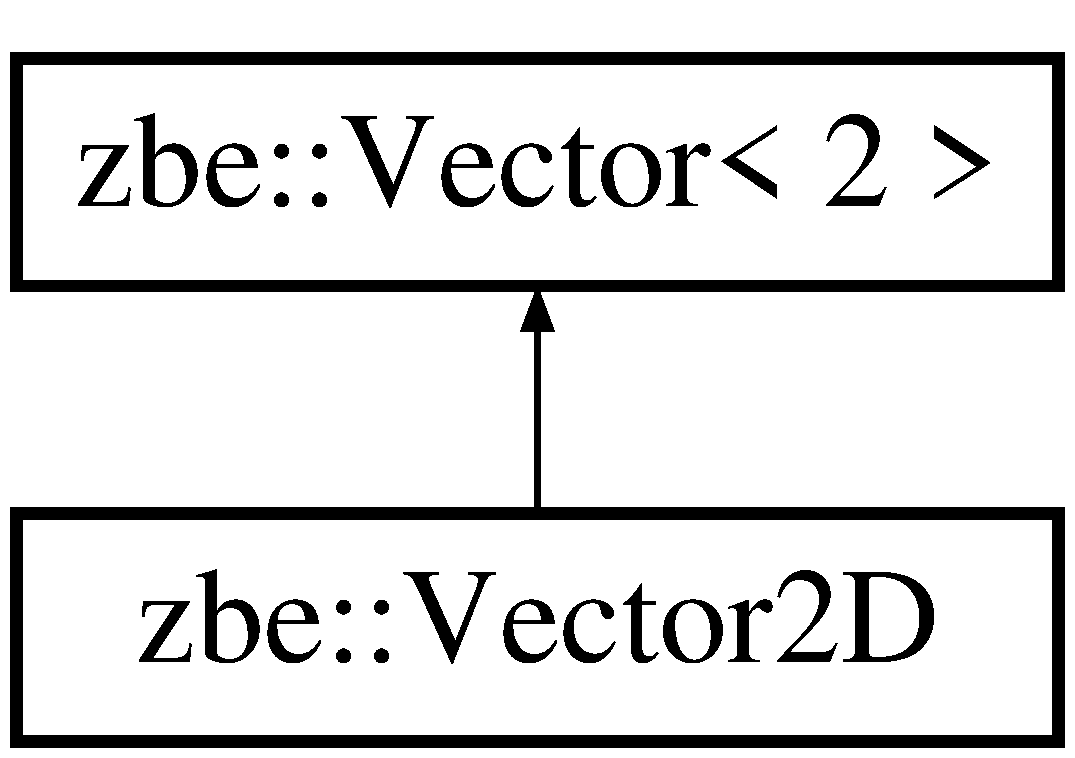
\includegraphics[height=2.000000cm]{classzbe_1_1_vector2_d}
\end{center}
\end{figure}
\subsection*{Public Member Functions}
\begin{DoxyCompactItemize}
\item 
\hyperlink{classzbe_1_1_vector2_d_a085719c80fc6468b80d8a5dd826b2cff}{Vector2\+D} ()
\begin{DoxyCompactList}\small\item\em Void constructor, the \hyperlink{classzbe_1_1_vector2_d}{Vector2\+D}\textquotesingle{}s values are unknown. \end{DoxyCompactList}\item 
\hyperlink{classzbe_1_1_vector2_d_a57f408da0866b7a65ba4afddbd12296b}{Vector2\+D} (const \hyperlink{classzbe_1_1_vector}{Vector}$<$ 2 $>$ \&v)
\begin{DoxyCompactList}\small\item\em A copy constructor with \hyperlink{classzbe_1_1_vector}{Vector$<$2$>$}. \end{DoxyCompactList}\item 
\hyperlink{classzbe_1_1_vector2_d_a5d0db3d7f9488739deece6ba1c0abd72}{Vector2\+D} (std\+::initializer\+\_\+list$<$ double $>$ l)
\begin{DoxyCompactList}\small\item\em A list initializer constructor. \end{DoxyCompactList}\item 
\hyperlink{classzbe_1_1_vector2_d}{Vector2\+D} \& \hyperlink{classzbe_1_1_vector2_d_aeaace85ca8133f1b56b4ce6b8db0ead1}{operator=} (\hyperlink{classzbe_1_1_vector}{Vector}$<$ 2 $>$ rhs)
\begin{DoxyCompactList}\small\item\em This class let you compare \hyperlink{classzbe_1_1_vector}{Vector$<$2$>$} with \hyperlink{classzbe_1_1_vector2_d}{Vector2\+D} classes. \end{DoxyCompactList}\item 
void \hyperlink{classzbe_1_1_vector2_d_a31df70571e1945f783fbcffdba992b16}{set\+Cartesian} (double \hyperlink{classzbe_1_1_vector2_d_a66e8c7ff408370756e48e2fd5f211b4e}{x}, double \hyperlink{classzbe_1_1_vector2_d_ab36f8d98268760d53da4efb305533cee}{y})
\begin{DoxyCompactList}\small\item\em Set values of the vector as Cartesian coordinates (default). \end{DoxyCompactList}\item 
void \hyperlink{classzbe_1_1_vector2_d_a652d41922aa9da7820b90ea5439f0457}{set\+Polars} (double r, double rads)
\begin{DoxyCompactList}\small\item\em Set values of the vector as Polar coordinates in radians (transformed to Cartesian). \end{DoxyCompactList}\item 
void \hyperlink{classzbe_1_1_vector2_d_a4d7f72ebfc41063239e63b0b36c156c4}{set\+Polars\+Degrees} (double r, double degree)
\begin{DoxyCompactList}\small\item\em Set values of the vector as Polar coordinates in degrees (transformed to Cartesian). \end{DoxyCompactList}\item 
double \hyperlink{classzbe_1_1_vector2_d_afb4af21a56128d64605b3bc8db0ed7a2}{get\+Rads} ()
\begin{DoxyCompactList}\small\item\em Get values of the Polar angles in radians (transformed from Cartesian). \end{DoxyCompactList}\item 
double \hyperlink{classzbe_1_1_vector2_d_ae39aff1de204d7295e126500d70e6a13}{get\+Degrees} ()
\begin{DoxyCompactList}\small\item\em Get values of the Polar angles in degrees (transformed from Cartesian). \end{DoxyCompactList}\end{DoxyCompactItemize}
\subsection*{Public Attributes}
\begin{DoxyCompactItemize}
\item 
double \& \hyperlink{classzbe_1_1_vector2_d_a66e8c7ff408370756e48e2fd5f211b4e}{x} = \hyperlink{classzbe_1_1_vector_a1adaf8d4244fe2c1d762d6c58f4b01eb}{data}\mbox{[}0\mbox{]}
\begin{DoxyCompactList}\small\item\em An alias to access the first dimension as v.\+x. \end{DoxyCompactList}\item 
double \& \hyperlink{classzbe_1_1_vector2_d_ab36f8d98268760d53da4efb305533cee}{y} = \hyperlink{classzbe_1_1_vector_a1adaf8d4244fe2c1d762d6c58f4b01eb}{data}\mbox{[}1\mbox{]}
\begin{DoxyCompactList}\small\item\em An alias to access the first dimension as v.\+y. \end{DoxyCompactList}\end{DoxyCompactItemize}
\subsection*{Additional Inherited Members}


\subsection{Detailed Description}
An aliases of a \hyperlink{classzbe_1_1_vector}{Vector$<$2$>$}. 

Used to implement some functionality of a 2 dimensional \hyperlink{classzbe_1_1_vector}{Vector}. 

Definition at line 236 of file Vector.\+h.



\subsection{Constructor \& Destructor Documentation}
\hypertarget{classzbe_1_1_vector2_d_a085719c80fc6468b80d8a5dd826b2cff}{}\index{zbe\+::\+Vector2\+D@{zbe\+::\+Vector2\+D}!Vector2\+D@{Vector2\+D}}
\index{Vector2\+D@{Vector2\+D}!zbe\+::\+Vector2\+D@{zbe\+::\+Vector2\+D}}
\subsubsection[{Vector2\+D()}]{\setlength{\rightskip}{0pt plus 5cm}zbe\+::\+Vector2\+D\+::\+Vector2\+D (
\begin{DoxyParamCaption}
{}
\end{DoxyParamCaption}
)\hspace{0.3cm}{\ttfamily [inline]}}\label{classzbe_1_1_vector2_d_a085719c80fc6468b80d8a5dd826b2cff}


Void constructor, the \hyperlink{classzbe_1_1_vector2_d}{Vector2\+D}\textquotesingle{}s values are unknown. 



Definition at line 243 of file Vector.\+h.

\hypertarget{classzbe_1_1_vector2_d_a57f408da0866b7a65ba4afddbd12296b}{}\index{zbe\+::\+Vector2\+D@{zbe\+::\+Vector2\+D}!Vector2\+D@{Vector2\+D}}
\index{Vector2\+D@{Vector2\+D}!zbe\+::\+Vector2\+D@{zbe\+::\+Vector2\+D}}
\subsubsection[{Vector2\+D(const Vector$<$ 2 $>$ \&v)}]{\setlength{\rightskip}{0pt plus 5cm}zbe\+::\+Vector2\+D\+::\+Vector2\+D (
\begin{DoxyParamCaption}
\item[{const {\bf Vector}$<$ 2 $>$ \&}]{v}
\end{DoxyParamCaption}
)\hspace{0.3cm}{\ttfamily [inline]}}\label{classzbe_1_1_vector2_d_a57f408da0866b7a65ba4afddbd12296b}


A copy constructor with \hyperlink{classzbe_1_1_vector}{Vector$<$2$>$}. 



Definition at line 247 of file Vector.\+h.

\hypertarget{classzbe_1_1_vector2_d_a5d0db3d7f9488739deece6ba1c0abd72}{}\index{zbe\+::\+Vector2\+D@{zbe\+::\+Vector2\+D}!Vector2\+D@{Vector2\+D}}
\index{Vector2\+D@{Vector2\+D}!zbe\+::\+Vector2\+D@{zbe\+::\+Vector2\+D}}
\subsubsection[{Vector2\+D(std\+::initializer\+\_\+list$<$ double $>$ l)}]{\setlength{\rightskip}{0pt plus 5cm}zbe\+::\+Vector2\+D\+::\+Vector2\+D (
\begin{DoxyParamCaption}
\item[{std\+::initializer\+\_\+list$<$ double $>$}]{l}
\end{DoxyParamCaption}
)\hspace{0.3cm}{\ttfamily [inline]}}\label{classzbe_1_1_vector2_d_a5d0db3d7f9488739deece6ba1c0abd72}


A list initializer constructor. 

You can create a \hyperlink{classzbe_1_1_vector2_d}{Vector2\+D} with a list of 2 values\+: \begin{DoxyVerb}  Vector2D v(v1, v2)
\end{DoxyVerb}


or \begin{DoxyVerb}  Vector2D v = {v1, v2}\end{DoxyVerb}
 

Definition at line 260 of file Vector.\+h.



\subsection{Member Function Documentation}
\hypertarget{classzbe_1_1_vector2_d_ae39aff1de204d7295e126500d70e6a13}{}\index{zbe\+::\+Vector2\+D@{zbe\+::\+Vector2\+D}!get\+Degrees@{get\+Degrees}}
\index{get\+Degrees@{get\+Degrees}!zbe\+::\+Vector2\+D@{zbe\+::\+Vector2\+D}}
\subsubsection[{get\+Degrees()}]{\setlength{\rightskip}{0pt plus 5cm}double zbe\+::\+Vector2\+D\+::get\+Degrees (
\begin{DoxyParamCaption}
{}
\end{DoxyParamCaption}
)\hspace{0.3cm}{\ttfamily [inline]}}\label{classzbe_1_1_vector2_d_ae39aff1de204d7295e126500d70e6a13}


Get values of the Polar angles in degrees (transformed from Cartesian). 



Definition at line 284 of file Vector.\+h.

\hypertarget{classzbe_1_1_vector2_d_afb4af21a56128d64605b3bc8db0ed7a2}{}\index{zbe\+::\+Vector2\+D@{zbe\+::\+Vector2\+D}!get\+Rads@{get\+Rads}}
\index{get\+Rads@{get\+Rads}!zbe\+::\+Vector2\+D@{zbe\+::\+Vector2\+D}}
\subsubsection[{get\+Rads()}]{\setlength{\rightskip}{0pt plus 5cm}double zbe\+::\+Vector2\+D\+::get\+Rads (
\begin{DoxyParamCaption}
{}
\end{DoxyParamCaption}
)\hspace{0.3cm}{\ttfamily [inline]}}\label{classzbe_1_1_vector2_d_afb4af21a56128d64605b3bc8db0ed7a2}


Get values of the Polar angles in radians (transformed from Cartesian). 



Definition at line 280 of file Vector.\+h.

\hypertarget{classzbe_1_1_vector2_d_aeaace85ca8133f1b56b4ce6b8db0ead1}{}\index{zbe\+::\+Vector2\+D@{zbe\+::\+Vector2\+D}!operator=@{operator=}}
\index{operator=@{operator=}!zbe\+::\+Vector2\+D@{zbe\+::\+Vector2\+D}}
\subsubsection[{operator=(\+Vector$<$ 2 $>$ rhs)}]{\setlength{\rightskip}{0pt plus 5cm}{\bf Vector2\+D}\& zbe\+::\+Vector2\+D\+::operator= (
\begin{DoxyParamCaption}
\item[{{\bf Vector}$<$ 2 $>$}]{rhs}
\end{DoxyParamCaption}
)\hspace{0.3cm}{\ttfamily [inline]}}\label{classzbe_1_1_vector2_d_aeaace85ca8133f1b56b4ce6b8db0ead1}


This class let you compare \hyperlink{classzbe_1_1_vector}{Vector$<$2$>$} with \hyperlink{classzbe_1_1_vector2_d}{Vector2\+D} classes. 



Definition at line 264 of file Vector.\+h.

\hypertarget{classzbe_1_1_vector2_d_a31df70571e1945f783fbcffdba992b16}{}\index{zbe\+::\+Vector2\+D@{zbe\+::\+Vector2\+D}!set\+Cartesian@{set\+Cartesian}}
\index{set\+Cartesian@{set\+Cartesian}!zbe\+::\+Vector2\+D@{zbe\+::\+Vector2\+D}}
\subsubsection[{set\+Cartesian(double x, double y)}]{\setlength{\rightskip}{0pt plus 5cm}void zbe\+::\+Vector2\+D\+::set\+Cartesian (
\begin{DoxyParamCaption}
\item[{double}]{x, }
\item[{double}]{y}
\end{DoxyParamCaption}
)\hspace{0.3cm}{\ttfamily [inline]}}\label{classzbe_1_1_vector2_d_a31df70571e1945f783fbcffdba992b16}


Set values of the vector as Cartesian coordinates (default). 



Definition at line 268 of file Vector.\+h.

\hypertarget{classzbe_1_1_vector2_d_a652d41922aa9da7820b90ea5439f0457}{}\index{zbe\+::\+Vector2\+D@{zbe\+::\+Vector2\+D}!set\+Polars@{set\+Polars}}
\index{set\+Polars@{set\+Polars}!zbe\+::\+Vector2\+D@{zbe\+::\+Vector2\+D}}
\subsubsection[{set\+Polars(double r, double rads)}]{\setlength{\rightskip}{0pt plus 5cm}void zbe\+::\+Vector2\+D\+::set\+Polars (
\begin{DoxyParamCaption}
\item[{double}]{r, }
\item[{double}]{rads}
\end{DoxyParamCaption}
)\hspace{0.3cm}{\ttfamily [inline]}}\label{classzbe_1_1_vector2_d_a652d41922aa9da7820b90ea5439f0457}


Set values of the vector as Polar coordinates in radians (transformed to Cartesian). 



Definition at line 272 of file Vector.\+h.

\hypertarget{classzbe_1_1_vector2_d_a4d7f72ebfc41063239e63b0b36c156c4}{}\index{zbe\+::\+Vector2\+D@{zbe\+::\+Vector2\+D}!set\+Polars\+Degrees@{set\+Polars\+Degrees}}
\index{set\+Polars\+Degrees@{set\+Polars\+Degrees}!zbe\+::\+Vector2\+D@{zbe\+::\+Vector2\+D}}
\subsubsection[{set\+Polars\+Degrees(double r, double degree)}]{\setlength{\rightskip}{0pt plus 5cm}void zbe\+::\+Vector2\+D\+::set\+Polars\+Degrees (
\begin{DoxyParamCaption}
\item[{double}]{r, }
\item[{double}]{degree}
\end{DoxyParamCaption}
)\hspace{0.3cm}{\ttfamily [inline]}}\label{classzbe_1_1_vector2_d_a4d7f72ebfc41063239e63b0b36c156c4}


Set values of the vector as Polar coordinates in degrees (transformed to Cartesian). 



Definition at line 276 of file Vector.\+h.



\subsection{Member Data Documentation}
\hypertarget{classzbe_1_1_vector2_d_a66e8c7ff408370756e48e2fd5f211b4e}{}\index{zbe\+::\+Vector2\+D@{zbe\+::\+Vector2\+D}!x@{x}}
\index{x@{x}!zbe\+::\+Vector2\+D@{zbe\+::\+Vector2\+D}}
\subsubsection[{x}]{\setlength{\rightskip}{0pt plus 5cm}double\& zbe\+::\+Vector2\+D\+::x = {\bf data}\mbox{[}0\mbox{]}}\label{classzbe_1_1_vector2_d_a66e8c7ff408370756e48e2fd5f211b4e}


An alias to access the first dimension as v.\+x. 



Definition at line 238 of file Vector.\+h.

\hypertarget{classzbe_1_1_vector2_d_ab36f8d98268760d53da4efb305533cee}{}\index{zbe\+::\+Vector2\+D@{zbe\+::\+Vector2\+D}!y@{y}}
\index{y@{y}!zbe\+::\+Vector2\+D@{zbe\+::\+Vector2\+D}}
\subsubsection[{y}]{\setlength{\rightskip}{0pt plus 5cm}double\& zbe\+::\+Vector2\+D\+::y = {\bf data}\mbox{[}1\mbox{]}}\label{classzbe_1_1_vector2_d_ab36f8d98268760d53da4efb305533cee}


An alias to access the first dimension as v.\+y. 



Definition at line 239 of file Vector.\+h.



The documentation for this class was generated from the following file\+:\begin{DoxyCompactItemize}
\item 
include/\+Z\+B\+E/core/tools/math/\hyperlink{_vector_8h}{Vector.\+h}\end{DoxyCompactItemize}

\hypertarget{classzbe_1_1_vector3_d}{}\section{zbe\+:\+:Vector3\+D Class Reference}
\label{classzbe_1_1_vector3_d}\index{zbe\+::\+Vector3\+D@{zbe\+::\+Vector3\+D}}


{\ttfamily \#include $<$Vector.\+h$>$}

Inheritance diagram for zbe\+:\+:Vector3\+D\+:\begin{figure}[H]
\begin{center}
\leavevmode
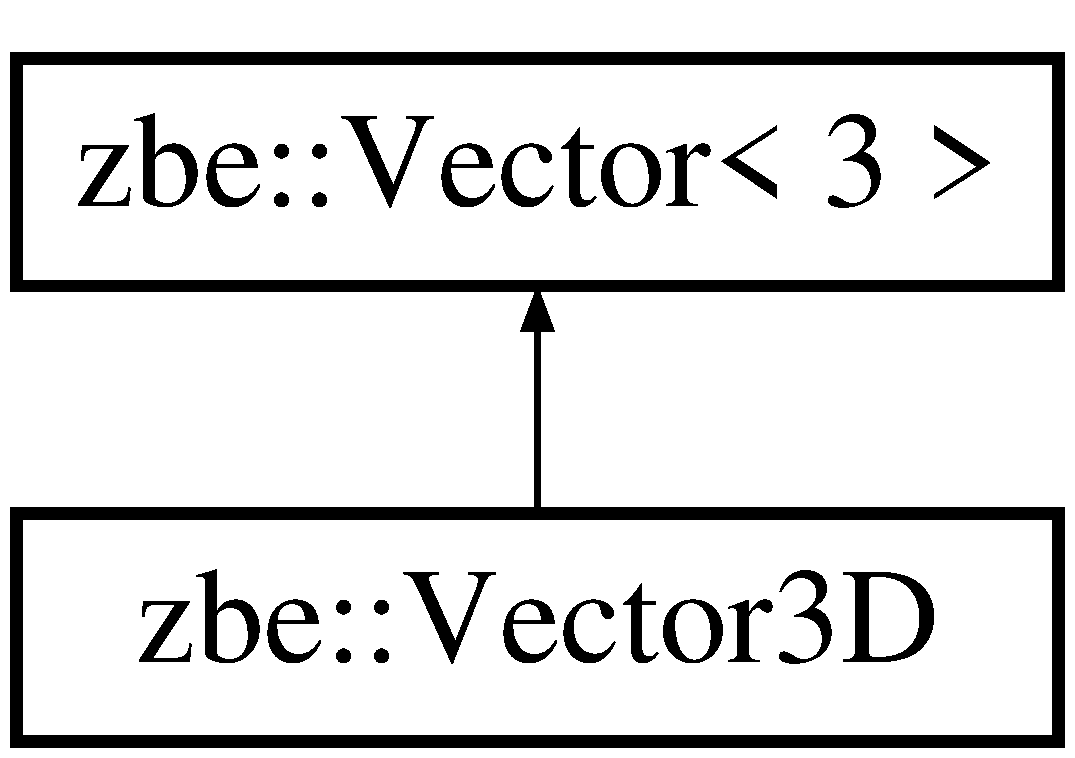
\includegraphics[height=2.000000cm]{classzbe_1_1_vector3_d}
\end{center}
\end{figure}
\subsection*{Public Member Functions}
\begin{DoxyCompactItemize}
\item 
\hyperlink{classzbe_1_1_vector3_d_a0d146ef6fbef42b6deb4515c249be745}{Vector3\+D} ()
\begin{DoxyCompactList}\small\item\em Void constructor, the \hyperlink{classzbe_1_1_vector3_d}{Vector3\+D}\textquotesingle{}s values are unknown. \end{DoxyCompactList}\item 
\hyperlink{classzbe_1_1_vector3_d_a44afbc2c1d8931955c60a0097a2d79eb}{Vector3\+D} (const \hyperlink{classzbe_1_1_vector}{Vector}$<$ 3 $>$ \&v)
\begin{DoxyCompactList}\small\item\em A copy constructor with \hyperlink{classzbe_1_1_vector}{Vector$<$3$>$}. \end{DoxyCompactList}\item 
\hyperlink{classzbe_1_1_vector3_d_a7d6e976edcc246ec0fc324702baa4de8}{Vector3\+D} (std\+::initializer\+\_\+list$<$ double $>$ l)
\begin{DoxyCompactList}\small\item\em A list initializer constructor. \end{DoxyCompactList}\item 
\hyperlink{classzbe_1_1_vector3_d}{Vector3\+D} \& \hyperlink{classzbe_1_1_vector3_d_a566d6b397c6e92ad804b56de7023b668}{operator=} (\hyperlink{classzbe_1_1_vector}{Vector}$<$ 3 $>$ rhs)
\begin{DoxyCompactList}\small\item\em This class let you compare \hyperlink{classzbe_1_1_vector}{Vector$<$3$>$} with \hyperlink{classzbe_1_1_vector3_d}{Vector3\+D} classes. \end{DoxyCompactList}\end{DoxyCompactItemize}
\subsection*{Public Attributes}
\begin{DoxyCompactItemize}
\item 
double \& \hyperlink{classzbe_1_1_vector3_d_aa469ac9ec2a2e09919b0eed33fcfc81c}{x} = \hyperlink{classzbe_1_1_vector_a1adaf8d4244fe2c1d762d6c58f4b01eb}{data}\mbox{[}0\mbox{]}
\begin{DoxyCompactList}\small\item\em An alias to access the first dimension as v.\+x. \end{DoxyCompactList}\item 
double \& \hyperlink{classzbe_1_1_vector3_d_a0c6f850b940c6eb85132db01490f108f}{y} = \hyperlink{classzbe_1_1_vector_a1adaf8d4244fe2c1d762d6c58f4b01eb}{data}\mbox{[}1\mbox{]}
\begin{DoxyCompactList}\small\item\em An alias to access the first dimension as v.\+y. \end{DoxyCompactList}\item 
double \& \hyperlink{classzbe_1_1_vector3_d_a165df2c9c8ab4cf1ebb322ecffc9efba}{z} = \hyperlink{classzbe_1_1_vector_a1adaf8d4244fe2c1d762d6c58f4b01eb}{data}\mbox{[}2\mbox{]}
\begin{DoxyCompactList}\small\item\em An alias to access the first dimension as v.\+z. \end{DoxyCompactList}\end{DoxyCompactItemize}
\subsection*{Additional Inherited Members}


\subsection{Detailed Description}


Definition at line 293 of file Vector.\+h.



\subsection{Constructor \& Destructor Documentation}
\hypertarget{classzbe_1_1_vector3_d_a0d146ef6fbef42b6deb4515c249be745}{}\index{zbe\+::\+Vector3\+D@{zbe\+::\+Vector3\+D}!Vector3\+D@{Vector3\+D}}
\index{Vector3\+D@{Vector3\+D}!zbe\+::\+Vector3\+D@{zbe\+::\+Vector3\+D}}
\subsubsection[{Vector3\+D()}]{\setlength{\rightskip}{0pt plus 5cm}zbe\+::\+Vector3\+D\+::\+Vector3\+D (
\begin{DoxyParamCaption}
{}
\end{DoxyParamCaption}
)\hspace{0.3cm}{\ttfamily [inline]}}\label{classzbe_1_1_vector3_d_a0d146ef6fbef42b6deb4515c249be745}


Void constructor, the \hyperlink{classzbe_1_1_vector3_d}{Vector3\+D}\textquotesingle{}s values are unknown. 



Definition at line 301 of file Vector.\+h.

\hypertarget{classzbe_1_1_vector3_d_a44afbc2c1d8931955c60a0097a2d79eb}{}\index{zbe\+::\+Vector3\+D@{zbe\+::\+Vector3\+D}!Vector3\+D@{Vector3\+D}}
\index{Vector3\+D@{Vector3\+D}!zbe\+::\+Vector3\+D@{zbe\+::\+Vector3\+D}}
\subsubsection[{Vector3\+D(const Vector$<$ 3 $>$ \&v)}]{\setlength{\rightskip}{0pt plus 5cm}zbe\+::\+Vector3\+D\+::\+Vector3\+D (
\begin{DoxyParamCaption}
\item[{const {\bf Vector}$<$ 3 $>$ \&}]{v}
\end{DoxyParamCaption}
)\hspace{0.3cm}{\ttfamily [inline]}}\label{classzbe_1_1_vector3_d_a44afbc2c1d8931955c60a0097a2d79eb}


A copy constructor with \hyperlink{classzbe_1_1_vector}{Vector$<$3$>$}. 



Definition at line 305 of file Vector.\+h.

\hypertarget{classzbe_1_1_vector3_d_a7d6e976edcc246ec0fc324702baa4de8}{}\index{zbe\+::\+Vector3\+D@{zbe\+::\+Vector3\+D}!Vector3\+D@{Vector3\+D}}
\index{Vector3\+D@{Vector3\+D}!zbe\+::\+Vector3\+D@{zbe\+::\+Vector3\+D}}
\subsubsection[{Vector3\+D(std\+::initializer\+\_\+list$<$ double $>$ l)}]{\setlength{\rightskip}{0pt plus 5cm}zbe\+::\+Vector3\+D\+::\+Vector3\+D (
\begin{DoxyParamCaption}
\item[{std\+::initializer\+\_\+list$<$ double $>$}]{l}
\end{DoxyParamCaption}
)\hspace{0.3cm}{\ttfamily [inline]}}\label{classzbe_1_1_vector3_d_a7d6e976edcc246ec0fc324702baa4de8}


A list initializer constructor. 

You can create a \hyperlink{classzbe_1_1_vector3_d}{Vector3\+D} with a list of 3 values\+: \begin{DoxyVerb}  Vector3D v(v1, v2, v3)
\end{DoxyVerb}


or \begin{DoxyVerb}  Vector3D v = {v1, v2, v3}\end{DoxyVerb}
 

Definition at line 318 of file Vector.\+h.



\subsection{Member Function Documentation}
\hypertarget{classzbe_1_1_vector3_d_a566d6b397c6e92ad804b56de7023b668}{}\index{zbe\+::\+Vector3\+D@{zbe\+::\+Vector3\+D}!operator=@{operator=}}
\index{operator=@{operator=}!zbe\+::\+Vector3\+D@{zbe\+::\+Vector3\+D}}
\subsubsection[{operator=(\+Vector$<$ 3 $>$ rhs)}]{\setlength{\rightskip}{0pt plus 5cm}{\bf Vector3\+D}\& zbe\+::\+Vector3\+D\+::operator= (
\begin{DoxyParamCaption}
\item[{{\bf Vector}$<$ 3 $>$}]{rhs}
\end{DoxyParamCaption}
)\hspace{0.3cm}{\ttfamily [inline]}}\label{classzbe_1_1_vector3_d_a566d6b397c6e92ad804b56de7023b668}


This class let you compare \hyperlink{classzbe_1_1_vector}{Vector$<$3$>$} with \hyperlink{classzbe_1_1_vector3_d}{Vector3\+D} classes. 



Definition at line 322 of file Vector.\+h.



\subsection{Member Data Documentation}
\hypertarget{classzbe_1_1_vector3_d_aa469ac9ec2a2e09919b0eed33fcfc81c}{}\index{zbe\+::\+Vector3\+D@{zbe\+::\+Vector3\+D}!x@{x}}
\index{x@{x}!zbe\+::\+Vector3\+D@{zbe\+::\+Vector3\+D}}
\subsubsection[{x}]{\setlength{\rightskip}{0pt plus 5cm}double\& zbe\+::\+Vector3\+D\+::x = {\bf data}\mbox{[}0\mbox{]}}\label{classzbe_1_1_vector3_d_aa469ac9ec2a2e09919b0eed33fcfc81c}


An alias to access the first dimension as v.\+x. 



Definition at line 295 of file Vector.\+h.

\hypertarget{classzbe_1_1_vector3_d_a0c6f850b940c6eb85132db01490f108f}{}\index{zbe\+::\+Vector3\+D@{zbe\+::\+Vector3\+D}!y@{y}}
\index{y@{y}!zbe\+::\+Vector3\+D@{zbe\+::\+Vector3\+D}}
\subsubsection[{y}]{\setlength{\rightskip}{0pt plus 5cm}double\& zbe\+::\+Vector3\+D\+::y = {\bf data}\mbox{[}1\mbox{]}}\label{classzbe_1_1_vector3_d_a0c6f850b940c6eb85132db01490f108f}


An alias to access the first dimension as v.\+y. 



Definition at line 296 of file Vector.\+h.

\hypertarget{classzbe_1_1_vector3_d_a165df2c9c8ab4cf1ebb322ecffc9efba}{}\index{zbe\+::\+Vector3\+D@{zbe\+::\+Vector3\+D}!z@{z}}
\index{z@{z}!zbe\+::\+Vector3\+D@{zbe\+::\+Vector3\+D}}
\subsubsection[{z}]{\setlength{\rightskip}{0pt plus 5cm}double\& zbe\+::\+Vector3\+D\+::z = {\bf data}\mbox{[}2\mbox{]}}\label{classzbe_1_1_vector3_d_a165df2c9c8ab4cf1ebb322ecffc9efba}


An alias to access the first dimension as v.\+z. 



Definition at line 297 of file Vector.\+h.



The documentation for this class was generated from the following file\+:\begin{DoxyCompactItemize}
\item 
include/\+Z\+B\+E/core/tools/math/\hyperlink{_vector_8h}{Vector.\+h}\end{DoxyCompactItemize}

\hypertarget{classzbe_1_1_window}{}\section{zbe\+:\+:Window Class Reference}
\label{classzbe_1_1_window}\index{zbe\+::\+Window@{zbe\+::\+Window}}


Used to create windows using S\+D\+L 2.\+0.  




{\ttfamily \#include $<$Window.\+h$>$}

\subsection*{Public Member Functions}
\begin{DoxyCompactItemize}
\item 
\hyperlink{classzbe_1_1_window_ae87c358f8fb31ce7f22475a881dc6530}{Window} (int width, int height, Uint32 window\+\_\+flags=0)
\item 
\hyperlink{classzbe_1_1_window_a27728e4d41f05485e0675b33d8f20200}{Window} (const char $\ast$title, int width, int height, Uint32 window\+\_\+flags=0, Uint32 rederer\+\_\+flags=0)
\item 
\hyperlink{classzbe_1_1_window_ace3681780598adf45a6eb23986d7ca28}{Window} (const char $\ast$title, int x, int y, int width, int height, Uint32 window\+\_\+flags=0, Uint32 rederer\+\_\+flags=0)
\item 
\hyperlink{classzbe_1_1_window_a5d4159697767615290b573a736289717}{$\sim$\+Window} ()
\item 
void \hyperlink{classzbe_1_1_window_acce2f3781015f07f4bceaedfdc532ef0}{clear} ()
\item 
void \hyperlink{classzbe_1_1_window_ab7a17f206733069edf81077158f8e716}{render} (S\+D\+L\+\_\+\+Texture $\ast$texture, const S\+D\+L\+\_\+\+Rect $\ast$srcrect, const S\+D\+L\+\_\+\+Rect $\ast$dstrect)
\item 
void \hyperlink{classzbe_1_1_window_a4279ab8613bdc10773eec0043b545259}{render} (S\+D\+L\+\_\+\+Texture $\ast$texture, const S\+D\+L\+\_\+\+Rect $\ast$srcrect, const S\+D\+L\+\_\+\+Rect $\ast$dstrect, const double angle, const S\+D\+L\+\_\+\+Point $\ast$center, const S\+D\+L\+\_\+\+Renderer\+Flip flip)
\item 
void \hyperlink{classzbe_1_1_window_a049d52d9e819193c17fe1f976d3f0c8c}{render} (unsigned tex\+I\+D, const S\+D\+L\+\_\+\+Rect $\ast$srcrect, const S\+D\+L\+\_\+\+Rect $\ast$dstrect)
\item 
void \hyperlink{classzbe_1_1_window_a522deb589562f9097d7b9be4cc2b0f5b}{render} (unsigned tex\+I\+D, const S\+D\+L\+\_\+\+Rect $\ast$srcrect, const S\+D\+L\+\_\+\+Rect $\ast$dstrect, const double angle, const S\+D\+L\+\_\+\+Point $\ast$center, const S\+D\+L\+\_\+\+Renderer\+Flip flip)
\item 
void \hyperlink{classzbe_1_1_window_adc44834dc0c4f32638487e3cfbd158b4}{present} ()
\item 
unsigned \hyperlink{classzbe_1_1_window_af5dec36e08941c5e8da92349d063d41b}{load\+Img} (const char $\ast$url)
\item 
unsigned \hyperlink{classzbe_1_1_window_ab08ebb55d0af8f844cfbd1c22d5faeb3}{reload\+Img} (const char $\ast$url, unsigned id)
\end{DoxyCompactItemize}


\subsection{Detailed Description}
Used to create windows using S\+D\+L 2.\+0. 

Definition at line 25 of file Window.\+h.



\subsection{Constructor \& Destructor Documentation}
\hypertarget{classzbe_1_1_window_ae87c358f8fb31ce7f22475a881dc6530}{}\index{zbe\+::\+Window@{zbe\+::\+Window}!Window@{Window}}
\index{Window@{Window}!zbe\+::\+Window@{zbe\+::\+Window}}
\subsubsection[{Window(int width, int height, Uint32 window\+\_\+flags=0)}]{\setlength{\rightskip}{0pt plus 5cm}zbe\+::\+Window\+::\+Window (
\begin{DoxyParamCaption}
\item[{int}]{width, }
\item[{int}]{height, }
\item[{Uint32}]{window\+\_\+flags = {\ttfamily 0}}
\end{DoxyParamCaption}
)}\label{classzbe_1_1_window_ae87c358f8fb31ce7f22475a881dc6530}
\hypertarget{classzbe_1_1_window_a27728e4d41f05485e0675b33d8f20200}{}\index{zbe\+::\+Window@{zbe\+::\+Window}!Window@{Window}}
\index{Window@{Window}!zbe\+::\+Window@{zbe\+::\+Window}}
\subsubsection[{Window(const char $\ast$title, int width, int height, Uint32 window\+\_\+flags=0, Uint32 rederer\+\_\+flags=0)}]{\setlength{\rightskip}{0pt plus 5cm}zbe\+::\+Window\+::\+Window (
\begin{DoxyParamCaption}
\item[{const char $\ast$}]{title, }
\item[{int}]{width, }
\item[{int}]{height, }
\item[{Uint32}]{window\+\_\+flags = {\ttfamily 0}, }
\item[{Uint32}]{rederer\+\_\+flags = {\ttfamily 0}}
\end{DoxyParamCaption}
)}\label{classzbe_1_1_window_a27728e4d41f05485e0675b33d8f20200}
\hypertarget{classzbe_1_1_window_ace3681780598adf45a6eb23986d7ca28}{}\index{zbe\+::\+Window@{zbe\+::\+Window}!Window@{Window}}
\index{Window@{Window}!zbe\+::\+Window@{zbe\+::\+Window}}
\subsubsection[{Window(const char $\ast$title, int x, int y, int width, int height, Uint32 window\+\_\+flags=0, Uint32 rederer\+\_\+flags=0)}]{\setlength{\rightskip}{0pt plus 5cm}zbe\+::\+Window\+::\+Window (
\begin{DoxyParamCaption}
\item[{const char $\ast$}]{title, }
\item[{int}]{x, }
\item[{int}]{y, }
\item[{int}]{width, }
\item[{int}]{height, }
\item[{Uint32}]{window\+\_\+flags = {\ttfamily 0}, }
\item[{Uint32}]{rederer\+\_\+flags = {\ttfamily 0}}
\end{DoxyParamCaption}
)}\label{classzbe_1_1_window_ace3681780598adf45a6eb23986d7ca28}
\hypertarget{classzbe_1_1_window_a5d4159697767615290b573a736289717}{}\index{zbe\+::\+Window@{zbe\+::\+Window}!````~Window@{$\sim$\+Window}}
\index{````~Window@{$\sim$\+Window}!zbe\+::\+Window@{zbe\+::\+Window}}
\subsubsection[{$\sim$\+Window()}]{\setlength{\rightskip}{0pt plus 5cm}zbe\+::\+Window\+::$\sim$\+Window (
\begin{DoxyParamCaption}
{}
\end{DoxyParamCaption}
)}\label{classzbe_1_1_window_a5d4159697767615290b573a736289717}


\subsection{Member Function Documentation}
\hypertarget{classzbe_1_1_window_acce2f3781015f07f4bceaedfdc532ef0}{}\index{zbe\+::\+Window@{zbe\+::\+Window}!clear@{clear}}
\index{clear@{clear}!zbe\+::\+Window@{zbe\+::\+Window}}
\subsubsection[{clear()}]{\setlength{\rightskip}{0pt plus 5cm}void zbe\+::\+Window\+::clear (
\begin{DoxyParamCaption}
{}
\end{DoxyParamCaption}
)}\label{classzbe_1_1_window_acce2f3781015f07f4bceaedfdc532ef0}
\hypertarget{classzbe_1_1_window_af5dec36e08941c5e8da92349d063d41b}{}\index{zbe\+::\+Window@{zbe\+::\+Window}!load\+Img@{load\+Img}}
\index{load\+Img@{load\+Img}!zbe\+::\+Window@{zbe\+::\+Window}}
\subsubsection[{load\+Img(const char $\ast$url)}]{\setlength{\rightskip}{0pt plus 5cm}unsigned zbe\+::\+Window\+::load\+Img (
\begin{DoxyParamCaption}
\item[{const char $\ast$}]{url}
\end{DoxyParamCaption}
)}\label{classzbe_1_1_window_af5dec36e08941c5e8da92349d063d41b}
\hypertarget{classzbe_1_1_window_adc44834dc0c4f32638487e3cfbd158b4}{}\index{zbe\+::\+Window@{zbe\+::\+Window}!present@{present}}
\index{present@{present}!zbe\+::\+Window@{zbe\+::\+Window}}
\subsubsection[{present()}]{\setlength{\rightskip}{0pt plus 5cm}void zbe\+::\+Window\+::present (
\begin{DoxyParamCaption}
{}
\end{DoxyParamCaption}
)\hspace{0.3cm}{\ttfamily [inline]}}\label{classzbe_1_1_window_adc44834dc0c4f32638487e3cfbd158b4}


Definition at line 41 of file Window.\+h.

\hypertarget{classzbe_1_1_window_ab08ebb55d0af8f844cfbd1c22d5faeb3}{}\index{zbe\+::\+Window@{zbe\+::\+Window}!reload\+Img@{reload\+Img}}
\index{reload\+Img@{reload\+Img}!zbe\+::\+Window@{zbe\+::\+Window}}
\subsubsection[{reload\+Img(const char $\ast$url, unsigned id)}]{\setlength{\rightskip}{0pt plus 5cm}unsigned zbe\+::\+Window\+::reload\+Img (
\begin{DoxyParamCaption}
\item[{const char $\ast$}]{url, }
\item[{unsigned}]{id}
\end{DoxyParamCaption}
)}\label{classzbe_1_1_window_ab08ebb55d0af8f844cfbd1c22d5faeb3}
\hypertarget{classzbe_1_1_window_ab7a17f206733069edf81077158f8e716}{}\index{zbe\+::\+Window@{zbe\+::\+Window}!render@{render}}
\index{render@{render}!zbe\+::\+Window@{zbe\+::\+Window}}
\subsubsection[{render(\+S\+D\+L\+\_\+\+Texture $\ast$texture, const S\+D\+L\+\_\+\+Rect $\ast$srcrect, const S\+D\+L\+\_\+\+Rect $\ast$dstrect)}]{\setlength{\rightskip}{0pt plus 5cm}void zbe\+::\+Window\+::render (
\begin{DoxyParamCaption}
\item[{S\+D\+L\+\_\+\+Texture $\ast$}]{texture, }
\item[{const S\+D\+L\+\_\+\+Rect $\ast$}]{srcrect, }
\item[{const S\+D\+L\+\_\+\+Rect $\ast$}]{dstrect}
\end{DoxyParamCaption}
)}\label{classzbe_1_1_window_ab7a17f206733069edf81077158f8e716}
\hypertarget{classzbe_1_1_window_a4279ab8613bdc10773eec0043b545259}{}\index{zbe\+::\+Window@{zbe\+::\+Window}!render@{render}}
\index{render@{render}!zbe\+::\+Window@{zbe\+::\+Window}}
\subsubsection[{render(\+S\+D\+L\+\_\+\+Texture $\ast$texture, const S\+D\+L\+\_\+\+Rect $\ast$srcrect, const S\+D\+L\+\_\+\+Rect $\ast$dstrect, const double angle, const S\+D\+L\+\_\+\+Point $\ast$center, const S\+D\+L\+\_\+\+Renderer\+Flip flip)}]{\setlength{\rightskip}{0pt plus 5cm}void zbe\+::\+Window\+::render (
\begin{DoxyParamCaption}
\item[{S\+D\+L\+\_\+\+Texture $\ast$}]{texture, }
\item[{const S\+D\+L\+\_\+\+Rect $\ast$}]{srcrect, }
\item[{const S\+D\+L\+\_\+\+Rect $\ast$}]{dstrect, }
\item[{const double}]{angle, }
\item[{const S\+D\+L\+\_\+\+Point $\ast$}]{center, }
\item[{const S\+D\+L\+\_\+\+Renderer\+Flip}]{flip}
\end{DoxyParamCaption}
)}\label{classzbe_1_1_window_a4279ab8613bdc10773eec0043b545259}
\hypertarget{classzbe_1_1_window_a049d52d9e819193c17fe1f976d3f0c8c}{}\index{zbe\+::\+Window@{zbe\+::\+Window}!render@{render}}
\index{render@{render}!zbe\+::\+Window@{zbe\+::\+Window}}
\subsubsection[{render(unsigned tex\+I\+D, const S\+D\+L\+\_\+\+Rect $\ast$srcrect, const S\+D\+L\+\_\+\+Rect $\ast$dstrect)}]{\setlength{\rightskip}{0pt plus 5cm}void zbe\+::\+Window\+::render (
\begin{DoxyParamCaption}
\item[{unsigned}]{tex\+I\+D, }
\item[{const S\+D\+L\+\_\+\+Rect $\ast$}]{srcrect, }
\item[{const S\+D\+L\+\_\+\+Rect $\ast$}]{dstrect}
\end{DoxyParamCaption}
)}\label{classzbe_1_1_window_a049d52d9e819193c17fe1f976d3f0c8c}
\hypertarget{classzbe_1_1_window_a522deb589562f9097d7b9be4cc2b0f5b}{}\index{zbe\+::\+Window@{zbe\+::\+Window}!render@{render}}
\index{render@{render}!zbe\+::\+Window@{zbe\+::\+Window}}
\subsubsection[{render(unsigned tex\+I\+D, const S\+D\+L\+\_\+\+Rect $\ast$srcrect, const S\+D\+L\+\_\+\+Rect $\ast$dstrect, const double angle, const S\+D\+L\+\_\+\+Point $\ast$center, const S\+D\+L\+\_\+\+Renderer\+Flip flip)}]{\setlength{\rightskip}{0pt plus 5cm}void zbe\+::\+Window\+::render (
\begin{DoxyParamCaption}
\item[{unsigned}]{tex\+I\+D, }
\item[{const S\+D\+L\+\_\+\+Rect $\ast$}]{srcrect, }
\item[{const S\+D\+L\+\_\+\+Rect $\ast$}]{dstrect, }
\item[{const double}]{angle, }
\item[{const S\+D\+L\+\_\+\+Point $\ast$}]{center, }
\item[{const S\+D\+L\+\_\+\+Renderer\+Flip}]{flip}
\end{DoxyParamCaption}
)}\label{classzbe_1_1_window_a522deb589562f9097d7b9be4cc2b0f5b}


The documentation for this class was generated from the following file\+:\begin{DoxyCompactItemize}
\item 
include/\+Z\+B\+E/core/\+S\+D\+L2.\+0/\hyperlink{_window_8h}{Window.\+h}\end{DoxyCompactItemize}

\chapter{File Documentation}
\hypertarget{_a_a_b_b_collisionable_8h}{}\section{include/\+Z\+B\+E/core/archetypes/\+A\+A\+B\+B\+Collisionable.h File Reference}
\label{_a_a_b_b_collisionable_8h}\index{include/\+Z\+B\+E/core/archetypes/\+A\+A\+B\+B\+Collisionable.\+h@{include/\+Z\+B\+E/core/archetypes/\+A\+A\+B\+B\+Collisionable.\+h}}


Define a class that collides as a Axis Aligned Bounding Box (A\+A\+B\+B).  


\subsection*{Classes}
\begin{DoxyCompactItemize}
\item 
class \hyperlink{classzbe_1_1_a_a_b_b_collisionable}{zbe\+::\+A\+A\+B\+B\+Collisionable}
\end{DoxyCompactItemize}
\subsection*{Namespaces}
\begin{DoxyCompactItemize}
\item 
 \hyperlink{namespacezbe}{zbe}
\end{DoxyCompactItemize}


\subsection{Detailed Description}
Define a class that collides as a Axis Aligned Bounding Box (A\+A\+B\+B). 

Copyright 2012 Batis Degryll Ludo

\begin{DoxySince}{Since}
2014-\/05-\/94 
\end{DoxySince}
\begin{DoxyDate}{Date}
2015-\/05-\/04 
\end{DoxyDate}
\begin{DoxyAuthor}{Author}
Degryll 
\end{DoxyAuthor}

\hypertarget{_a_a_b_b_sphere_collisionable_8h}{}\section{include/\+Z\+B\+E/core/archetypes/\+A\+A\+B\+B\+Sphere\+Collisionable.h File Reference}
\label{_a_a_b_b_sphere_collisionable_8h}\index{include/\+Z\+B\+E/core/archetypes/\+A\+A\+B\+B\+Sphere\+Collisionable.\+h@{include/\+Z\+B\+E/core/archetypes/\+A\+A\+B\+B\+Sphere\+Collisionable.\+h}}


Define a class that Collides hierarchically as a sphere and in more detail as an A\+A\+B\+B.  


\subsection*{Classes}
\begin{DoxyCompactItemize}
\item 
class \hyperlink{classzbe_1_1_a_a_b_b_sphere_collisionable}{zbe\+::\+A\+A\+B\+B\+Sphere\+Collisionable}
\end{DoxyCompactItemize}
\subsection*{Namespaces}
\begin{DoxyCompactItemize}
\item 
 \hyperlink{namespacezbe}{zbe}
\end{DoxyCompactItemize}


\subsection{Detailed Description}
Define a class that Collides hierarchically as a sphere and in more detail as an A\+A\+B\+B. 

Copyright 2012 Batis Degryll Ludo

\begin{DoxySince}{Since}
2014-\/05-\/94 
\end{DoxySince}
\begin{DoxyDate}{Date}
2015-\/05-\/04 
\end{DoxyDate}
\begin{DoxyAuthor}{Author}
Degryll 
\end{DoxyAuthor}

\hypertarget{_collisionable_8h}{}\section{include/\+Z\+B\+E/core/archetypes/\+Collisionable.h File Reference}
\label{_collisionable_8h}\index{include/\+Z\+B\+E/core/archetypes/\+Collisionable.\+h@{include/\+Z\+B\+E/core/archetypes/\+Collisionable.\+h}}


Define a class that participate in collision system.  


{\ttfamily \#include \char`\"{}Z\+B\+E/core/tools/math/\+Vector2\+D.\+h\char`\"{}}\\*
\subsection*{Classes}
\begin{DoxyCompactItemize}
\item 
class \hyperlink{classzbe_1_1_collisionable}{zbe\+::\+Collisionable}
\end{DoxyCompactItemize}
\subsection*{Namespaces}
\begin{DoxyCompactItemize}
\item 
 \hyperlink{namespacezbe}{zbe}
\end{DoxyCompactItemize}


\subsection{Detailed Description}
Define a class that participate in collision system. 

Copyright 2012 Batis Degryll Ludo

\begin{DoxySince}{Since}
2014-\/09-\/22 
\end{DoxySince}
\begin{DoxyDate}{Date}
2014-\/09-\/22 
\end{DoxyDate}
\begin{DoxyAuthor}{Author}
Ludo and Degryll 
\end{DoxyAuthor}

\hypertarget{_collisionador_8h}{}\section{include/\+Z\+B\+E/core/archetypes/\+Collisionador.h File Reference}
\label{_collisionador_8h}\index{include/\+Z\+B\+E/core/archetypes/\+Collisionador.\+h@{include/\+Z\+B\+E/core/archetypes/\+Collisionador.\+h}}


Define a class that participate in collision system.  


{\ttfamily \#include \char`\"{}Z\+B\+E/core/tools/math/collisions/\+Collision\+Data.\+h\char`\"{}}\\*
\subsection*{Classes}
\begin{DoxyCompactItemize}
\item 
class \hyperlink{classzbe_1_1_collisionador}{zbe\+::\+Collisionador}
\end{DoxyCompactItemize}
\subsection*{Namespaces}
\begin{DoxyCompactItemize}
\item 
 \hyperlink{namespacezbe}{zbe}
\end{DoxyCompactItemize}


\subsection{Detailed Description}
Define a class that participate in collision system. 

Copyright 2012 Batis Degryll Ludo

\begin{DoxySince}{Since}
2014-\/09-\/22 
\end{DoxySince}
\begin{DoxyDate}{Date}
2014-\/09-\/22 
\end{DoxyDate}
\begin{DoxyAuthor}{Author}
Ludo and Degryll 
\end{DoxyAuthor}

\hypertarget{_collisioner_8h}{}\section{include/\+Z\+B\+E/core/archetypes/\+Collisioner.h File Reference}
\label{_collisioner_8h}\index{include/\+Z\+B\+E/core/archetypes/\+Collisioner.\+h@{include/\+Z\+B\+E/core/archetypes/\+Collisioner.\+h}}


Define a class that participate in collision system.  


{\ttfamily \#include \char`\"{}Z\+B\+E/core/tools/math/\+Vector.\+h\char`\"{}}\\*
\subsection*{Classes}
\begin{DoxyCompactItemize}
\item 
class \hyperlink{classzbe_1_1_collisioner}{zbe\+::\+Collisioner}
\end{DoxyCompactItemize}
\subsection*{Namespaces}
\begin{DoxyCompactItemize}
\item 
 \hyperlink{namespacezbe}{zbe}
\end{DoxyCompactItemize}


\subsection{Detailed Description}
Define a class that participate in collision system. 

Copyright 2012 Batis Degryll Ludo

\begin{DoxySince}{Since}
2014-\/09-\/12 
\end{DoxySince}
\begin{DoxyDate}{Date}
2014-\/09-\/12 
\end{DoxyDate}
\begin{DoxyAuthor}{Author}
Ludo and Degryll 
\end{DoxyAuthor}

\hypertarget{_movable_8h}{}\section{include/\+Z\+B\+E/core/archetypes/\+Movable.h File Reference}
\label{_movable_8h}\index{include/\+Z\+B\+E/core/archetypes/\+Movable.\+h@{include/\+Z\+B\+E/core/archetypes/\+Movable.\+h}}
{\ttfamily \#include \char`\"{}Z\+B\+E/core/archetypes/\+Positionable.\+h\char`\"{}}\\*
{\ttfamily \#include \char`\"{}Z\+B\+E/core/tools/math/\+Vector.\+h\char`\"{}}\\*
\subsection*{Classes}
\begin{DoxyCompactItemize}
\item 
class \hyperlink{classzbe_1_1_movable}{zbe\+::\+Movable$<$ s $>$}
\end{DoxyCompactItemize}
\subsection*{Namespaces}
\begin{DoxyCompactItemize}
\item 
 \hyperlink{namespacezbe}{zbe}
\end{DoxyCompactItemize}

\hypertarget{_positionable_8h}{}\section{include/\+Z\+B\+E/core/archetypes/\+Positionable.h File Reference}
\label{_positionable_8h}\index{include/\+Z\+B\+E/core/archetypes/\+Positionable.\+h@{include/\+Z\+B\+E/core/archetypes/\+Positionable.\+h}}


Define a class that has a position in the world.  


{\ttfamily \#include \char`\"{}Z\+B\+E/core/tools/math/\+Vector.\+h\char`\"{}}\\*
{\ttfamily \#include \char`\"{}Z\+B\+E/core/tools/math/\+Point.\+h\char`\"{}}\\*
\subsection*{Classes}
\begin{DoxyCompactItemize}
\item 
class \hyperlink{classzbe_1_1_positionable}{zbe\+::\+Positionable$<$ s $>$}
\end{DoxyCompactItemize}
\subsection*{Namespaces}
\begin{DoxyCompactItemize}
\item 
 \hyperlink{namespacezbe}{zbe}
\end{DoxyCompactItemize}


\subsection{Detailed Description}
Define a class that has a position in the world. 

Copyright 2012 Batis Degryll Ludo

\begin{DoxySince}{Since}
2015-\/05-\/04 
\end{DoxySince}
\begin{DoxyDate}{Date}
2015-\/05-\/04 
\end{DoxyDate}
\begin{DoxyAuthor}{Author}
Degryll 
\end{DoxyAuthor}

\hypertarget{_runnable_8h}{}\section{include/\+Z\+B\+E/core/archetypes/\+Runnable.h File Reference}
\label{_runnable_8h}\index{include/\+Z\+B\+E/core/archetypes/\+Runnable.\+h@{include/\+Z\+B\+E/core/archetypes/\+Runnable.\+h}}


Define a class with a void run(void) function.  


\subsection*{Classes}
\begin{DoxyCompactItemize}
\item 
class \hyperlink{classzbe_1_1_runnable}{zbe\+::\+Runnable}
\end{DoxyCompactItemize}
\subsection*{Namespaces}
\begin{DoxyCompactItemize}
\item 
 \hyperlink{namespacezbe}{zbe}
\end{DoxyCompactItemize}


\subsection{Detailed Description}
Define a class with a void run(void) function. 

Copyright 2012 Batis Degryll Ludo

\begin{DoxySince}{Since}
2014-\/09-\/08 
\end{DoxySince}
\begin{DoxyDate}{Date}
2014-\/09-\/08 
\end{DoxyDate}
\begin{DoxyAuthor}{Author}
Ludo and Degryll 
\end{DoxyAuthor}

\hypertarget{_simple_sprite_8h}{}\section{include/\+Z\+B\+E/core/archetypes/\+Simple\+Sprite.h File Reference}
\label{_simple_sprite_8h}\index{include/\+Z\+B\+E/core/archetypes/\+Simple\+Sprite.\+h@{include/\+Z\+B\+E/core/archetypes/\+Simple\+Sprite.\+h}}


Define a class that can be draw as a simple sprite.  


{\ttfamily \#include $<$S\+D\+L2/\+S\+D\+L.\+h$>$}\\*
\subsection*{Classes}
\begin{DoxyCompactItemize}
\item 
class \hyperlink{classzbe_1_1_simple_sprite}{zbe\+::\+Simple\+Sprite}
\end{DoxyCompactItemize}
\subsection*{Namespaces}
\begin{DoxyCompactItemize}
\item 
 \hyperlink{namespacezbe}{zbe}
\end{DoxyCompactItemize}


\subsection{Detailed Description}
Define a class that can be draw as a simple sprite. 

Copyright 2012 Batis Degryll Ludo

\begin{DoxySince}{Since}
2014-\/09-\/27 
\end{DoxySince}
\begin{DoxyDate}{Date}
2015-\/05-\/04 
\end{DoxyDate}
\begin{DoxyAuthor}{Author}
Ludo and Degryll 
\end{DoxyAuthor}

\hypertarget{_sphere_collisionable_8h}{}\section{include/\+Z\+B\+E/core/archetypes/\+Sphere\+Collisionable.h File Reference}
\label{_sphere_collisionable_8h}\index{include/\+Z\+B\+E/core/archetypes/\+Sphere\+Collisionable.\+h@{include/\+Z\+B\+E/core/archetypes/\+Sphere\+Collisionable.\+h}}


Define a class that collides as a sphere.  


\subsection*{Classes}
\begin{DoxyCompactItemize}
\item 
class \hyperlink{classzbe_1_1_sphere_collisionable}{zbe\+::\+Sphere\+Collisionable}
\end{DoxyCompactItemize}
\subsection*{Namespaces}
\begin{DoxyCompactItemize}
\item 
 \hyperlink{namespacezbe}{zbe}
\end{DoxyCompactItemize}


\subsection{Detailed Description}
Define a class that collides as a sphere. 

Copyright 2012 Batis Degryll Ludo

\begin{DoxySince}{Since}
2014-\/05-\/04 
\end{DoxySince}
\begin{DoxyDate}{Date}
2015-\/05-\/04 
\end{DoxyDate}
\begin{DoxyAuthor}{Author}
Degryll 
\end{DoxyAuthor}

\hypertarget{_behavior_8h}{}\section{include/\+Z\+B\+E/core/behaviors/\+Behavior.h File Reference}
\label{_behavior_8h}\index{include/\+Z\+B\+E/core/behaviors/\+Behavior.\+h@{include/\+Z\+B\+E/core/behaviors/\+Behavior.\+h}}


Define the minimal functions of every behavior.  


\subsection*{Classes}
\begin{DoxyCompactItemize}
\item 
class \hyperlink{classzbe_1_1_behavior}{zbe\+::\+Behavior}
\end{DoxyCompactItemize}
\subsection*{Namespaces}
\begin{DoxyCompactItemize}
\item 
 \hyperlink{namespacezbe}{zbe}
\end{DoxyCompactItemize}


\subsection{Detailed Description}
Define the minimal functions of every behavior. 

Define the minimal functions of demons.

Copyright 2012 Batis Degryll Ludo

\begin{DoxySince}{Since}
2014-\/09-\/12 
\end{DoxySince}
\begin{DoxyDate}{Date}
2015-\/05-\/04 
\end{DoxyDate}
\begin{DoxyAuthor}{Author}
Ludo and Degryll
\end{DoxyAuthor}
Copyright 2015 Batis Degryll Ludo

\begin{DoxySince}{Since}
2014-\/09-\/12 
\end{DoxySince}
\begin{DoxyDate}{Date}
2015-\/05-\/04 
\end{DoxyDate}
\begin{DoxyAuthor}{Author}
Ludo 
\end{DoxyAuthor}

\hypertarget{_uniform_linear_motion_8h}{}\section{include/\+Z\+B\+E/core/behaviors/\+Uniform\+Linear\+Motion.h File Reference}
\label{_uniform_linear_motion_8h}\index{include/\+Z\+B\+E/core/behaviors/\+Uniform\+Linear\+Motion.\+h@{include/\+Z\+B\+E/core/behaviors/\+Uniform\+Linear\+Motion.\+h}}


Updates the position of an object based on its speed. Requires Movible.  


{\ttfamily \#include \char`\"{}any\+\_\+iterator.\+hpp\char`\"{}}\\*
{\ttfamily \#include \char`\"{}Z\+B\+E/core/behaviors/\+Behavior.\+h\char`\"{}}\\*
{\ttfamily \#include \char`\"{}Z\+B\+E/core/archetypes/\+Movable.\+h\char`\"{}}\\*
\subsection*{Classes}
\begin{DoxyCompactItemize}
\item 
class \hyperlink{classzbe_1_1_uniform_linear_motion}{zbe\+::\+Uniform\+Linear\+Motion$<$ s $>$}
\end{DoxyCompactItemize}
\subsection*{Namespaces}
\begin{DoxyCompactItemize}
\item 
 \hyperlink{namespacezbe}{zbe}
\end{DoxyCompactItemize}
\subsection*{Typedefs}
\begin{DoxyCompactItemize}
\item 
{\footnotesize template$<$unsigned s$>$ }\\using \hyperlink{namespacezbe_aac207741b7b7b641e92f8eac56a8fd88}{zbe\+::\+Movable\+Iterator} = Iterator\+Type\+Erasure\+::any\+\_\+iterator$<$ Movable$<$ s $>$, boost\+::forward\+\_\+traversal\+\_\+tag, Movable$<$ s $>$ \&, ptrdiff\+\_\+t $>$
\end{DoxyCompactItemize}


\subsection{Detailed Description}
Updates the position of an object based on its speed. Requires Movible. 

Copyright 2012 Batis Degryll Ludo

\begin{DoxySince}{Since}
2015-\/05-\/04 
\end{DoxySince}
\begin{DoxyDate}{Date}
2015-\/05-\/04 
\end{DoxyDate}
\begin{DoxyAuthor}{Author}
Degryll 
\end{DoxyAuthor}

\hypertarget{_daemon_8h}{}\section{include/\+Z\+B\+E/core/daemons/\+Daemon.h File Reference}
\label{_daemon_8h}\index{include/\+Z\+B\+E/core/daemons/\+Daemon.\+h@{include/\+Z\+B\+E/core/daemons/\+Daemon.\+h}}
\subsection*{Classes}
\begin{DoxyCompactItemize}
\item 
class \hyperlink{class_daemon}{Daemon}
\end{DoxyCompactItemize}

\hypertarget{_daemon_master_8h}{}\section{include/\+Z\+B\+E/core/daemons/\+Daemon\+Master.h File Reference}
\label{_daemon_master_8h}\index{include/\+Z\+B\+E/core/daemons/\+Daemon\+Master.\+h@{include/\+Z\+B\+E/core/daemons/\+Daemon\+Master.\+h}}
{\ttfamily \#include $<$vector$>$}\\*
{\ttfamily \#include \char`\"{}./\+Daemon.\+h\char`\"{}}\\*
\subsection*{Classes}
\begin{DoxyCompactItemize}
\item 
class \hyperlink{classzbe_1_1_daemon_master}{zbe\+::\+Daemon\+Master}
\end{DoxyCompactItemize}
\subsection*{Namespaces}
\begin{DoxyCompactItemize}
\item 
 \hyperlink{namespacezbe}{zbe}
\end{DoxyCompactItemize}

\hypertarget{_drawer_8h}{}\section{include/\+Z\+B\+E/core/drawers/\+Drawer.h File Reference}
\label{_drawer_8h}\index{include/\+Z\+B\+E/core/drawers/\+Drawer.\+h@{include/\+Z\+B\+E/core/drawers/\+Drawer.\+h}}


Define the minimal functions of every Drawer.  


\subsection*{Classes}
\begin{DoxyCompactItemize}
\item 
class \hyperlink{classzbe_1_1_drawer}{zbe\+::\+Drawer}
\end{DoxyCompactItemize}
\subsection*{Namespaces}
\begin{DoxyCompactItemize}
\item 
 \hyperlink{namespacezbe}{zbe}
\end{DoxyCompactItemize}


\subsection{Detailed Description}
Define the minimal functions of every Drawer. 

Copyright 2012 Batis Degryll Ludo

\begin{DoxySince}{Since}
2014-\/09-\/22 
\end{DoxySince}
\begin{DoxyDate}{Date}
2014-\/09-\/27 
\end{DoxyDate}
\begin{DoxyAuthor}{Author}
Ludo and Degryll 
\end{DoxyAuthor}

\hypertarget{_simple_sprite_s_d_l_drawer_8h}{}\section{include/\+Z\+B\+E/core/drawers/\+S\+D\+L/\+Simple\+Sprite\+S\+D\+L\+Drawer.h File Reference}
\label{_simple_sprite_s_d_l_drawer_8h}\index{include/\+Z\+B\+E/core/drawers/\+S\+D\+L/\+Simple\+Sprite\+S\+D\+L\+Drawer.\+h@{include/\+Z\+B\+E/core/drawers/\+S\+D\+L/\+Simple\+Sprite\+S\+D\+L\+Drawer.\+h}}


Class that know how to draw Simple\+Sprite entities with S\+D\+L.  


{\ttfamily \#include \char`\"{}Z\+B\+E/core/drawers/\+Drawer.\+h\char`\"{}}\\*
{\ttfamily \#include \char`\"{}Z\+B\+E/core/archetypes/\+Simple\+Sprite.\+h\char`\"{}}\\*
{\ttfamily \#include \char`\"{}Z\+B\+E/core/\+S\+D\+L2.\+0/\+Window.\+h\char`\"{}}\\*
{\ttfamily \#include \char`\"{}any\+\_\+iterator.\+hpp\char`\"{}}\\*
{\ttfamily \#include $<$S\+D\+L2/\+S\+D\+L.\+h$>$}\\*
\subsection*{Classes}
\begin{DoxyCompactItemize}
\item 
class \hyperlink{classzbe_1_1_simple_sprite_s_d_l_drawer}{zbe\+::\+Simple\+Sprite\+S\+D\+L\+Drawer}
\end{DoxyCompactItemize}
\subsection*{Namespaces}
\begin{DoxyCompactItemize}
\item 
 \hyperlink{namespacezbe}{zbe}
\end{DoxyCompactItemize}
\subsection*{Typedefs}
\begin{DoxyCompactItemize}
\item 
typedef Iterator\+Type\+Erasure\+::any\+\_\+iterator$<$ Simple\+Sprite, boost\+::forward\+\_\+traversal\+\_\+tag, Simple\+Sprite \&, ptrdiff\+\_\+t $>$ \hyperlink{namespacezbe_aa6d4affc7b95360c2d43d5fde9837a1f}{zbe\+::\+Simple\+Sprite\+Iterator}
\end{DoxyCompactItemize}


\subsection{Detailed Description}
Class that know how to draw Simple\+Sprite entities with S\+D\+L. 

Copyright 2012 Batis Degryll Ludo

\begin{DoxySince}{Since}
2012-\/02-\/01 
\end{DoxySince}
\begin{DoxyDate}{Date}
2014-\/09-\/27 
\end{DoxyDate}
\begin{DoxyAuthor}{Author}
degryll 
\end{DoxyAuthor}

\hypertarget{_file_handler_8h}{}\section{include/\+Z\+B\+E/core/io/\+File\+Handler.h File Reference}
\label{_file_handler_8h}\index{include/\+Z\+B\+E/core/io/\+File\+Handler.\+h@{include/\+Z\+B\+E/core/io/\+File\+Handler.\+h}}


To handle files.  


{\ttfamily \#include $<$string$>$}\\*
\subsection*{Classes}
\begin{DoxyCompactItemize}
\item 
class \hyperlink{classzbe_1_1_file_handler}{zbe\+::\+File\+Handler}
\end{DoxyCompactItemize}
\subsection*{Namespaces}
\begin{DoxyCompactItemize}
\item 
 \hyperlink{namespacezbe}{zbe}
\end{DoxyCompactItemize}


\subsection{Detailed Description}
To handle files. 

Copyright 2012 Batis Degryll Ludo

\begin{DoxySince}{Since}
2014-\/05-\/25 
\end{DoxySince}
\begin{DoxyDate}{Date}
2014-\/08-\/23 
\end{DoxyDate}
\begin{DoxyAuthor}{Author}
Degryll 
\end{DoxyAuthor}

\hypertarget{_s_d_l_font_loader_8h}{}\section{include/\+Z\+B\+E/core/loaders/\+S\+D\+L\+Font\+Loader.h File Reference}
\label{_s_d_l_font_loader_8h}\index{include/\+Z\+B\+E/core/loaders/\+S\+D\+L\+Font\+Loader.\+h@{include/\+Z\+B\+E/core/loaders/\+S\+D\+L\+Font\+Loader.\+h}}
{\ttfamily \#include $<$S\+D\+L2/\+S\+D\+L\+\_\+ttf.\+h$>$}\\*
{\ttfamily \#include $<$map$>$}\\*
\subsection*{Classes}
\begin{DoxyCompactItemize}
\item 
class \hyperlink{classzbe_1_1_s_d_l_font_loader}{zbe\+::\+S\+D\+L\+Font\+Loader}
\end{DoxyCompactItemize}
\subsection*{Namespaces}
\begin{DoxyCompactItemize}
\item 
 \hyperlink{namespacezbe}{zbe}
\end{DoxyCompactItemize}

\hypertarget{_window_8h}{}\section{include/\+Z\+B\+E/core/\+S\+D\+L2.0/\+Window.h File Reference}
\label{_window_8h}\index{include/\+Z\+B\+E/core/\+S\+D\+L2.\+0/\+Window.\+h@{include/\+Z\+B\+E/core/\+S\+D\+L2.\+0/\+Window.\+h}}
{\ttfamily \#include $<$vector$>$}\\*
{\ttfamily \#include $<$mutex$>$}\\*
{\ttfamily \#include $<$S\+D\+L2/\+S\+D\+L.\+h$>$}\\*
\subsection*{Classes}
\begin{DoxyCompactItemize}
\item 
class \hyperlink{classzbe_1_1_window}{zbe\+::\+Window}
\begin{DoxyCompactList}\small\item\em Used to create windows using S\+D\+L 2.\+0. \end{DoxyCompactList}\end{DoxyCompactItemize}
\subsection*{Namespaces}
\begin{DoxyCompactItemize}
\item 
 \hyperlink{namespacezbe}{zbe}
\end{DoxyCompactItemize}

\hypertarget{_s_d_l___starter_8h}{}\section{include/\+Z\+B\+E/core/starters/\+S\+D\+L\+\_\+\+Starter.h File Reference}
\label{_s_d_l___starter_8h}\index{include/\+Z\+B\+E/core/starters/\+S\+D\+L\+\_\+\+Starter.\+h@{include/\+Z\+B\+E/core/starters/\+S\+D\+L\+\_\+\+Starter.\+h}}
{\ttfamily \#include $<$S\+D\+L2/\+S\+D\+L.\+h$>$}\\*
\subsection*{Classes}
\begin{DoxyCompactItemize}
\item 
class \hyperlink{classzbe_1_1_s_d_l___starter}{zbe\+::\+S\+D\+L\+\_\+\+Starter}
\begin{DoxyCompactList}\small\item\em Used to init S\+D\+L subsystems only once (alonelton). \end{DoxyCompactList}\end{DoxyCompactItemize}
\subsection*{Namespaces}
\begin{DoxyCompactItemize}
\item 
 \hyperlink{namespacezbe}{zbe}
\end{DoxyCompactItemize}

\hypertarget{_app_8h}{}\section{include/\+Z\+B\+E/core/system/\+App.h File Reference}
\label{_app_8h}\index{include/\+Z\+B\+E/core/system/\+App.\+h@{include/\+Z\+B\+E/core/system/\+App.\+h}}


Main application.  


{\ttfamily \#include \char`\"{}Z\+B\+E/core/archetypes/\+Runnable.\+h\char`\"{}}\\*
\subsection*{Classes}
\begin{DoxyCompactItemize}
\item 
class \hyperlink{classzbe_1_1_app}{zbe\+::\+App}
\end{DoxyCompactItemize}
\subsection*{Namespaces}
\begin{DoxyCompactItemize}
\item 
 \hyperlink{namespacezbe}{zbe}
\end{DoxyCompactItemize}


\subsection{Detailed Description}
Main application. 

Copyright 2012 Batis Degryll Ludo

\begin{DoxySince}{Since}
2014-\/09-\/08 
\end{DoxySince}
\begin{DoxyDate}{Date}
2014-\/09-\/09 
\end{DoxyDate}
\begin{DoxyAuthor}{Author}
Ludo and Degryll 
\end{DoxyAuthor}

\hypertarget{_game_app_8h}{}\section{include/\+Z\+B\+E/core/system/\+Game\+App.h File Reference}
\label{_game_app_8h}\index{include/\+Z\+B\+E/core/system/\+Game\+App.\+h@{include/\+Z\+B\+E/core/system/\+Game\+App.\+h}}


Main game application.  


{\ttfamily \#include $<$forward\+\_\+list$>$}\\*
{\ttfamily \#include $<$algorithm$>$}\\*
{\ttfamily \#include \char`\"{}any\+\_\+iterator.\+hpp\char`\"{}}\\*
{\ttfamily \#include \char`\"{}Z\+B\+E/core/system/\+App.\+h\char`\"{}}\\*
{\ttfamily \#include \char`\"{}Z\+B\+E/core/\+Timer.\+h\char`\"{}}\\*
{\ttfamily \#include \char`\"{}Z\+B\+E/core/\+Collision\+Data.\+h\char`\"{}}\\*
{\ttfamily \#include \char`\"{}Z\+B\+E/core/\+Behavior.\+h\char`\"{}}\\*
{\ttfamily \#include \char`\"{}Z\+B\+E/core/\+Drawer.\+h\char`\"{}}\\*
\subsection*{Classes}
\begin{DoxyCompactItemize}
\item 
class \hyperlink{classzbe_1_1_game_app}{zbe\+::\+Game\+App}
\end{DoxyCompactItemize}
\subsection*{Namespaces}
\begin{DoxyCompactItemize}
\item 
 \hyperlink{namespacezbe}{zbe}
\end{DoxyCompactItemize}
\subsection*{Typedefs}
\begin{DoxyCompactItemize}
\item 
typedef Iterator\+Type\+Erasure\+::any\+\_\+iterator$<$ Behavior, boost\+::forward\+\_\+traversal\+\_\+tag, Behavior \&, ptrdiff\+\_\+t $>$ \hyperlink{namespacezbe_a98051e0b03810ff1bbe41c451aa7568e}{zbe\+::\+Behavior\+Iterator}
\item 
typedef Iterator\+Type\+Erasure\+::any\+\_\+iterator$<$ Collisioner, boost\+::forward\+\_\+traversal\+\_\+tag, Collisioner \&, ptrdiff\+\_\+t $>$ \hyperlink{namespacezbe_a38ddb97c007548db7c49a709eafb7b2e}{zbe\+::\+Collisioner\+Iterator}
\item 
typedef Iterator\+Type\+Erasure\+::any\+\_\+iterator$<$ Drawer, boost\+::forward\+\_\+traversal\+\_\+tag, Drawer \&, ptrdiff\+\_\+t $>$ \hyperlink{namespacezbe_a5d3dda3dc1f2ee13116b4c5958a47f2f}{zbe\+::\+Drawer\+Iterator}
\end{DoxyCompactItemize}


\subsection{Detailed Description}
Main game application. 

Data of a collision.

Copyright 2012 Batis Degryll Ludo

\begin{DoxySince}{Since}
2014-\/09-\/09 
\end{DoxySince}
\begin{DoxyDate}{Date}
2014-\/09-\/22 
\end{DoxyDate}
\begin{DoxyAuthor}{Author}
Degryll
\end{DoxyAuthor}
Copyright 2012 Batis Degryll Ludo

\begin{DoxySince}{Since}
2014-\/09-\/12 
\end{DoxySince}
\begin{DoxyDate}{Date}
2014-\/09-\/12 
\end{DoxyDate}
\begin{DoxyAuthor}{Author}
Degryll 
\end{DoxyAuthor}

\hypertarget{_logger_8h}{}\section{include/\+Z\+B\+E/core/system/\+Logger.h File Reference}
\label{_logger_8h}\index{include/\+Z\+B\+E/core/system/\+Logger.\+h@{include/\+Z\+B\+E/core/system/\+Logger.\+h}}


To create Logs.  


{\ttfamily \#include $<$vector$>$}\\*
{\ttfamily \#include $<$forward\+\_\+list$>$}\\*
{\ttfamily \#include $<$string$>$}\\*
{\ttfamily \#include $<$sstream$>$}\\*
{\ttfamily \#include $<$mutex$>$}\\*
\subsection*{Classes}
\begin{DoxyCompactItemize}
\item 
class \hyperlink{classzbe_1_1_logger_msg}{zbe\+::\+Logger\+Msg}
\begin{DoxyCompactList}\small\item\em Wrapper class to use the operator \char`\"{}$<$$<$\char`\"{} in the log messages. \end{DoxyCompactList}\item 
class \hyperlink{classzbe_1_1_logger}{zbe\+::\+Logger}
\begin{DoxyCompactList}\small\item\em A class to handle logs. \end{DoxyCompactList}\end{DoxyCompactItemize}
\subsection*{Namespaces}
\begin{DoxyCompactItemize}
\item 
 \hyperlink{namespacezbe}{zbe}
\end{DoxyCompactItemize}
\subsection*{Macros}
\begin{DoxyCompactItemize}
\item 
\#define \hyperlink{_logger_8h_aea637f7a5ceb1e47013610d365595634}{Z\+B\+E\+\_\+\+L\+O\+G\+\_\+\+I\+N\+F\+O}(M\+S\+G)
\begin{DoxyCompactList}\small\item\em Add a \mbox{[}I\+N\+F\+O\mbox{]} annotation to the logs. \end{DoxyCompactList}\item 
\#define \hyperlink{_logger_8h_a8704b8bde1fad7b530734b70ab7e152a}{Z\+B\+E\+\_\+\+L\+O\+G\+\_\+\+D\+E\+B\+U\+G}(M\+S\+G)
\begin{DoxyCompactList}\small\item\em Add a \mbox{[}D\+E\+B\+U\+G\mbox{]} annotation to the logs. \end{DoxyCompactList}\item 
\#define \hyperlink{_logger_8h_a430ab0c478a3ca182053b637cf310e2a}{Z\+B\+E\+\_\+\+L\+O\+G\+\_\+\+W\+A\+R\+N\+I\+N\+G}(M\+S\+G)
\begin{DoxyCompactList}\small\item\em Add a \mbox{[}W\+A\+R\+N\+I\+N\+G\mbox{]} annotation to the logs. \end{DoxyCompactList}\item 
\#define \hyperlink{_logger_8h_a892ae22564bc52ef9ab2e7f0a3fe685b}{Z\+B\+E\+\_\+\+L\+O\+G\+\_\+\+E\+R\+R\+O\+R}(M\+S\+G)
\begin{DoxyCompactList}\small\item\em Add a \mbox{[}E\+R\+R\+O\+R\mbox{]} annotation to the logs. \end{DoxyCompactList}\item 
\#define \hyperlink{_logger_8h_a5e9327e95d0334514b212936d9e22672}{Z\+B\+E\+\_\+\+L\+O\+G\+\_\+\+O\+T\+H\+E\+R}(M\+S\+G\+T\+Y\+P\+E,  M\+S\+G)
\begin{DoxyCompactList}\small\item\em Add an user defined annotation to the logs. \end{DoxyCompactList}\item 
\#define \hyperlink{_logger_8h_ae7ed7d8c8b4553579d64206520feca76}{Z\+B\+E\+\_\+\+L\+O\+G}(N\+T\+Y\+P\+E,  M\+S\+G\+T\+Y\+P\+E,  M\+S\+G)
\begin{DoxyCompactList}\small\item\em Add an user defined annotation to the logs. \end{DoxyCompactList}\end{DoxyCompactItemize}


\subsection{Detailed Description}
To create Logs. 

Copyright 2012 Batis Degryll Ludo

\begin{DoxySince}{Since}
2014-\/05-\/16 
\end{DoxySince}
\begin{DoxyDate}{Date}
2015-\/10-\/24 
\end{DoxyDate}
\begin{DoxyAuthor}{Author}
Degryll 
\end{DoxyAuthor}


\subsection{Macro Definition Documentation}
\hypertarget{_logger_8h_ae7ed7d8c8b4553579d64206520feca76}{}\index{Logger.\+h@{Logger.\+h}!Z\+B\+E\+\_\+\+L\+O\+G@{Z\+B\+E\+\_\+\+L\+O\+G}}
\index{Z\+B\+E\+\_\+\+L\+O\+G@{Z\+B\+E\+\_\+\+L\+O\+G}!Logger.\+h@{Logger.\+h}}
\subsubsection[{Z\+B\+E\+\_\+\+L\+O\+G}]{\setlength{\rightskip}{0pt plus 5cm}\#define Z\+B\+E\+\_\+\+L\+O\+G(
\begin{DoxyParamCaption}
\item[{}]{N\+T\+Y\+P\+E, }
\item[{}]{M\+S\+G\+T\+Y\+P\+E, }
\item[{}]{M\+S\+G}
\end{DoxyParamCaption}
)}\label{_logger_8h_ae7ed7d8c8b4553579d64206520feca76}
{\bfseries Value\+:}
\begin{DoxyCode}
\textcolor{keywordflow}{do}\{ \hyperlink{classzbe_1_1_logger_msg}{zbe::LoggerMsg} lm; \(\backslash\)
    zbe::Logger::getInstance()->log(NTYPE, MSGTYPE, lm << \textcolor{stringliteral}{"> "} << MSG); \} \textcolor{keywordflow}{while}(0)
\end{DoxyCode}


Add an user defined annotation to the logs. 

Used to add messages to the logs with custom type (\mbox{[}T\+Y\+P\+E\mbox{]}) and type number (N\+T\+Y\+P\+E). 

Definition at line 64 of file Logger.\+h.

\hypertarget{_logger_8h_a8704b8bde1fad7b530734b70ab7e152a}{}\index{Logger.\+h@{Logger.\+h}!Z\+B\+E\+\_\+\+L\+O\+G\+\_\+\+D\+E\+B\+U\+G@{Z\+B\+E\+\_\+\+L\+O\+G\+\_\+\+D\+E\+B\+U\+G}}
\index{Z\+B\+E\+\_\+\+L\+O\+G\+\_\+\+D\+E\+B\+U\+G@{Z\+B\+E\+\_\+\+L\+O\+G\+\_\+\+D\+E\+B\+U\+G}!Logger.\+h@{Logger.\+h}}
\subsubsection[{Z\+B\+E\+\_\+\+L\+O\+G\+\_\+\+D\+E\+B\+U\+G}]{\setlength{\rightskip}{0pt plus 5cm}\#define Z\+B\+E\+\_\+\+L\+O\+G\+\_\+\+D\+E\+B\+U\+G(
\begin{DoxyParamCaption}
\item[{}]{M\+S\+G}
\end{DoxyParamCaption}
)}\label{_logger_8h_a8704b8bde1fad7b530734b70ab7e152a}
{\bfseries Value\+:}
\begin{DoxyCode}
\textcolor{keywordflow}{do}\{ \hyperlink{classzbe_1_1_logger_msg}{zbe::LoggerMsg} lm; \(\backslash\)
    zbe::Logger::getInstance()->log(\hyperlink{classzbe_1_1_logger_a33ad8282f2667bd086686ee3afa877d8}{zbe::Logger::NDEBUG}, 
      \hyperlink{classzbe_1_1_logger_a3b3e816024fb94bacee114109ce2c462}{zbe::Logger::TDEBUG}, lm << \_\_FILE\_\_ << \textcolor{stringliteral}{":"} << \_\_LINE\_\_ << \textcolor{stringliteral}{"> "} << MSG); \} \textcolor{keywordflow}{while}(0)
\end{DoxyCode}


Add a \mbox{[}D\+E\+B\+U\+G\mbox{]} annotation to the logs. 

Used to add debug messages to the logs, this annotation also include the file and line where the message comes from. 

Definition at line 32 of file Logger.\+h.

\hypertarget{_logger_8h_a892ae22564bc52ef9ab2e7f0a3fe685b}{}\index{Logger.\+h@{Logger.\+h}!Z\+B\+E\+\_\+\+L\+O\+G\+\_\+\+E\+R\+R\+O\+R@{Z\+B\+E\+\_\+\+L\+O\+G\+\_\+\+E\+R\+R\+O\+R}}
\index{Z\+B\+E\+\_\+\+L\+O\+G\+\_\+\+E\+R\+R\+O\+R@{Z\+B\+E\+\_\+\+L\+O\+G\+\_\+\+E\+R\+R\+O\+R}!Logger.\+h@{Logger.\+h}}
\subsubsection[{Z\+B\+E\+\_\+\+L\+O\+G\+\_\+\+E\+R\+R\+O\+R}]{\setlength{\rightskip}{0pt plus 5cm}\#define Z\+B\+E\+\_\+\+L\+O\+G\+\_\+\+E\+R\+R\+O\+R(
\begin{DoxyParamCaption}
\item[{}]{M\+S\+G}
\end{DoxyParamCaption}
)}\label{_logger_8h_a892ae22564bc52ef9ab2e7f0a3fe685b}
{\bfseries Value\+:}
\begin{DoxyCode}
\textcolor{keywordflow}{do}\{ \hyperlink{classzbe_1_1_logger_msg}{zbe::LoggerMsg} lm; \(\backslash\)
    zbe::Logger::getInstance()->log(\hyperlink{classzbe_1_1_logger_a78cd96d72ec926945b9a90f4d120ca28}{zbe::Logger::NERROR}, 
      \hyperlink{classzbe_1_1_logger_ac0b85a476489ca300a423ddbd1419040}{zbe::Logger::TERROR}, lm << \textcolor{stringliteral}{"> "} << MSG); \} \textcolor{keywordflow}{while}(0)
\end{DoxyCode}


Add a \mbox{[}E\+R\+R\+O\+R\mbox{]} annotation to the logs. 

Used to add error messages to the logs. 

Definition at line 48 of file Logger.\+h.

\hypertarget{_logger_8h_aea637f7a5ceb1e47013610d365595634}{}\index{Logger.\+h@{Logger.\+h}!Z\+B\+E\+\_\+\+L\+O\+G\+\_\+\+I\+N\+F\+O@{Z\+B\+E\+\_\+\+L\+O\+G\+\_\+\+I\+N\+F\+O}}
\index{Z\+B\+E\+\_\+\+L\+O\+G\+\_\+\+I\+N\+F\+O@{Z\+B\+E\+\_\+\+L\+O\+G\+\_\+\+I\+N\+F\+O}!Logger.\+h@{Logger.\+h}}
\subsubsection[{Z\+B\+E\+\_\+\+L\+O\+G\+\_\+\+I\+N\+F\+O}]{\setlength{\rightskip}{0pt plus 5cm}\#define Z\+B\+E\+\_\+\+L\+O\+G\+\_\+\+I\+N\+F\+O(
\begin{DoxyParamCaption}
\item[{}]{M\+S\+G}
\end{DoxyParamCaption}
)}\label{_logger_8h_aea637f7a5ceb1e47013610d365595634}
{\bfseries Value\+:}
\begin{DoxyCode}
\textcolor{keywordflow}{do}\{ \hyperlink{classzbe_1_1_logger_msg}{zbe::LoggerMsg} lm; \(\backslash\)
    zbe::Logger::getInstance()->log(\hyperlink{classzbe_1_1_logger_ad30e9493ec117daa24977bfa4cc883f1}{zbe::Logger::NINFO}, 
      \hyperlink{classzbe_1_1_logger_a90a7ec362737bacdfb922582cb7e142f}{zbe::Logger::TINFO}, lm << \textcolor{stringliteral}{"> "} << MSG); \} \textcolor{keywordflow}{while}(0)
\end{DoxyCode}


Add a \mbox{[}I\+N\+F\+O\mbox{]} annotation to the logs. 

Used to add information messages to the logs. 

Definition at line 23 of file Logger.\+h.

\hypertarget{_logger_8h_a5e9327e95d0334514b212936d9e22672}{}\index{Logger.\+h@{Logger.\+h}!Z\+B\+E\+\_\+\+L\+O\+G\+\_\+\+O\+T\+H\+E\+R@{Z\+B\+E\+\_\+\+L\+O\+G\+\_\+\+O\+T\+H\+E\+R}}
\index{Z\+B\+E\+\_\+\+L\+O\+G\+\_\+\+O\+T\+H\+E\+R@{Z\+B\+E\+\_\+\+L\+O\+G\+\_\+\+O\+T\+H\+E\+R}!Logger.\+h@{Logger.\+h}}
\subsubsection[{Z\+B\+E\+\_\+\+L\+O\+G\+\_\+\+O\+T\+H\+E\+R}]{\setlength{\rightskip}{0pt plus 5cm}\#define Z\+B\+E\+\_\+\+L\+O\+G\+\_\+\+O\+T\+H\+E\+R(
\begin{DoxyParamCaption}
\item[{}]{M\+S\+G\+T\+Y\+P\+E, }
\item[{}]{M\+S\+G}
\end{DoxyParamCaption}
)}\label{_logger_8h_a5e9327e95d0334514b212936d9e22672}
{\bfseries Value\+:}
\begin{DoxyCode}
\textcolor{keywordflow}{do}\{ \hyperlink{classzbe_1_1_logger_msg}{zbe::LoggerMsg} lm; \(\backslash\)
    zbe::Logger::getInstance()->log(-1,MSGTYPE, lm << \textcolor{stringliteral}{"> "} << MSG); \} \textcolor{keywordflow}{while}(0)
\end{DoxyCode}


Add an user defined annotation to the logs. 

Used to add messages to the logs with custom type (\mbox{[}T\+Y\+P\+E\mbox{]}). 

Definition at line 56 of file Logger.\+h.

\hypertarget{_logger_8h_a430ab0c478a3ca182053b637cf310e2a}{}\index{Logger.\+h@{Logger.\+h}!Z\+B\+E\+\_\+\+L\+O\+G\+\_\+\+W\+A\+R\+N\+I\+N\+G@{Z\+B\+E\+\_\+\+L\+O\+G\+\_\+\+W\+A\+R\+N\+I\+N\+G}}
\index{Z\+B\+E\+\_\+\+L\+O\+G\+\_\+\+W\+A\+R\+N\+I\+N\+G@{Z\+B\+E\+\_\+\+L\+O\+G\+\_\+\+W\+A\+R\+N\+I\+N\+G}!Logger.\+h@{Logger.\+h}}
\subsubsection[{Z\+B\+E\+\_\+\+L\+O\+G\+\_\+\+W\+A\+R\+N\+I\+N\+G}]{\setlength{\rightskip}{0pt plus 5cm}\#define Z\+B\+E\+\_\+\+L\+O\+G\+\_\+\+W\+A\+R\+N\+I\+N\+G(
\begin{DoxyParamCaption}
\item[{}]{M\+S\+G}
\end{DoxyParamCaption}
)}\label{_logger_8h_a430ab0c478a3ca182053b637cf310e2a}
{\bfseries Value\+:}
\begin{DoxyCode}
\textcolor{keywordflow}{do}\{ \hyperlink{classzbe_1_1_logger_msg}{zbe::LoggerMsg} lm; \(\backslash\)
    zbe::Logger::getInstance()->log(\hyperlink{classzbe_1_1_logger_aba8b4f2b50b95b7df8475cd3cf5584b9}{zbe::Logger::NWARNING}, 
      \hyperlink{classzbe_1_1_logger_a9dbd65ebc9452231ee1a0adaa3c08d93}{zbe::Logger::TWARNING}, lm << \textcolor{stringliteral}{"> "} << MSG); \} \textcolor{keywordflow}{while}(0)
\end{DoxyCode}


Add a \mbox{[}W\+A\+R\+N\+I\+N\+G\mbox{]} annotation to the logs. 

Used to add warning messages to the logs. 

Definition at line 40 of file Logger.\+h.


\hypertarget{_sys_error_8h}{}\section{include/\+Z\+B\+E/core/system/\+Sys\+Error.h File Reference}
\label{_sys_error_8h}\index{include/\+Z\+B\+E/core/system/\+Sys\+Error.\+h@{include/\+Z\+B\+E/core/system/\+Sys\+Error.\+h}}


A system class to inform about errors.  


{\ttfamily \#include $<$string$>$}\\*
\subsection*{Classes}
\begin{DoxyCompactItemize}
\item 
class \hyperlink{classzbe_1_1_sys_error}{zbe\+::\+Sys\+Error}
\begin{DoxyCompactList}\small\item\em A system class to inform about errors. \end{DoxyCompactList}\end{DoxyCompactItemize}
\subsection*{Namespaces}
\begin{DoxyCompactItemize}
\item 
 \hyperlink{namespacezbe}{zbe}
\end{DoxyCompactItemize}


\subsection{Detailed Description}
A system class to inform about errors. 

Copyright 2012 Batis Degryll Ludo

\begin{DoxySince}{Since}
2013-\/11-\/23 
\end{DoxySince}
\begin{DoxyDate}{Date}
2015-\/10-\/21 
\end{DoxyDate}
\begin{DoxyAuthor}{Author}
Degryll 
\end{DoxyAuthor}

\hypertarget{_array_list_8h}{}\section{include/\+Z\+B\+E/core/tools/containers/\+Array\+List.h File Reference}
\label{_array_list_8h}\index{include/\+Z\+B\+E/core/tools/containers/\+Array\+List.\+h@{include/\+Z\+B\+E/core/tools/containers/\+Array\+List.\+h}}


A list in an static array.  


{\ttfamily \#include \char`\"{}Z\+B\+E/core/system/\+Sys\+Error.\+h\char`\"{}}\\*
{\ttfamily \#include \char`\"{}Z\+B\+E/core/tools/containers/\+Ticket.\+h\char`\"{}}\\*
{\ttfamily \#include \char`\"{}Z\+B\+E/core/tools/containers/\+Array\+List\+Iterator.\+h\char`\"{}}\\*
\subsection*{Classes}
\begin{DoxyCompactItemize}
\item 
class \hyperlink{classzbe_1_1_array_list_iter}{zbe\+::\+Array\+List\+Iter$<$ Value $>$}
\item 
struct \hyperlink{structzbe_1_1_array_list_node}{zbe\+::\+Array\+List\+Node$<$ Value $>$}
\item 
class \hyperlink{classzbe_1_1_array_list}{zbe\+::\+Array\+List$<$ Value $>$}
\item 
class \hyperlink{classzbe_1_1_array_list_ticketed_iter}{zbe\+::\+Array\+List\+Ticketed\+Iter$<$ Value $>$}
\item 
struct \hyperlink{structzbe_1_1_array_list_ticketed_node}{zbe\+::\+Array\+List\+Ticketed\+Node$<$ Value $>$}
\item 
class \hyperlink{classzbe_1_1_array_list_ticketed}{zbe\+::\+Array\+List\+Ticketed$<$ Value $>$}
\end{DoxyCompactItemize}
\subsection*{Namespaces}
\begin{DoxyCompactItemize}
\item 
 \hyperlink{namespacezbe}{zbe}
\end{DoxyCompactItemize}


\subsection{Detailed Description}
A list in an static array. 

Copyright 2011 Batis Degryll Ludo

\begin{DoxySince}{Since}
2015/02/08 
\end{DoxySince}
\begin{DoxyDate}{Date}
2015/04/03 
\end{DoxyDate}
\begin{DoxyAuthor}{Author}
Degryll 
\end{DoxyAuthor}

\hypertarget{_array_list_iterator_8h}{}\section{include/\+Z\+B\+E/core/tools/containers/\+Array\+List\+Iterator.h File Reference}
\label{_array_list_iterator_8h}\index{include/\+Z\+B\+E/core/tools/containers/\+Array\+List\+Iterator.\+h@{include/\+Z\+B\+E/core/tools/containers/\+Array\+List\+Iterator.\+h}}


An iterator for the array\+List.  


{\ttfamily \#include $<$cstdio$>$}\\*
{\ttfamily \#include $<$boost/iterator/iterator\+\_\+facade.\+hpp$>$}\\*
{\ttfamily \#include \char`\"{}array\+List.\+h\char`\"{}}\\*
{\ttfamily \#include \char`\"{}Ticket.\+h\char`\"{}}\\*
\subsection*{Classes}
\begin{DoxyCompactItemize}
\item 
struct \hyperlink{structzbe_1_1_array_list_node}{zbe\+::\+Array\+List\+Node$<$ Value $>$}
\item 
class \hyperlink{classzbe_1_1_array_list}{zbe\+::\+Array\+List$<$ Value $>$}
\item 
class \hyperlink{classzbe_1_1_array_list_iter}{zbe\+::\+Array\+List\+Iter$<$ Value $>$}
\item 
struct \hyperlink{structzbe_1_1_array_list_ticketed_node}{zbe\+::\+Array\+List\+Ticketed\+Node$<$ Value $>$}
\item 
class \hyperlink{classzbe_1_1_array_list_ticketed}{zbe\+::\+Array\+List\+Ticketed$<$ Value $>$}
\item 
class \hyperlink{classzbe_1_1_array_list_ticketed_iter}{zbe\+::\+Array\+List\+Ticketed\+Iter$<$ Value $>$}
\end{DoxyCompactItemize}
\subsection*{Namespaces}
\begin{DoxyCompactItemize}
\item 
 \hyperlink{namespacezbe}{zbe}
\end{DoxyCompactItemize}
\subsection*{Typedefs}
\begin{DoxyCompactItemize}
\item 
{\footnotesize template$<$typename T $>$ }\\using \hyperlink{namespacezbe_af0d8ed46769e5212c0baa5ae5190e604}{zbe\+::\+Array\+List\+Iterator} = Array\+List\+Iter$<$ T $>$
\item 
{\footnotesize template$<$typename T $>$ }\\using \hyperlink{namespacezbe_ad150b3b2832337d2dce4e58c3fe7da58}{zbe\+::\+Array\+List\+Const\+Iterator} = Array\+List\+Iter$<$ T const  $>$
\item 
{\footnotesize template$<$typename T $>$ }\\using \hyperlink{namespacezbe_a1675a0090f0cdd995282757bb5f5bdbe}{zbe\+::\+Array\+List\+Ticketed\+Iterator} = Array\+List\+Ticketed\+Iter$<$ T $>$
\item 
{\footnotesize template$<$typename T $>$ }\\using \hyperlink{namespacezbe_afa10c72425dcc83afff52e7f290a1aee}{zbe\+::\+Array\+List\+Ticketed\+Const\+Iterator} = Array\+List\+Ticketed\+Iter$<$ T const  $>$
\end{DoxyCompactItemize}


\subsection{Detailed Description}
An iterator for the array\+List. 

Copyright 2011 Batis Degryll Ludo

\begin{DoxySince}{Since}
2015/02/08 
\end{DoxySince}
\begin{DoxyDate}{Date}
2015/04/10 
\end{DoxyDate}
\begin{DoxyAuthor}{Author}
Degryll 
\end{DoxyAuthor}

\hypertarget{_ticket_8h}{}\section{include/\+Z\+B\+E/core/tools/containers/\+Ticket.h File Reference}
\label{_ticket_8h}\index{include/\+Z\+B\+E/core/tools/containers/\+Ticket.\+h@{include/\+Z\+B\+E/core/tools/containers/\+Ticket.\+h}}


To be used in containers in witch each element can be marked as active, inactive, erase.  


\subsection*{Classes}
\begin{DoxyCompactItemize}
\item 
class \hyperlink{classzbe_1_1_ticket}{zbe\+::\+Ticket}
\end{DoxyCompactItemize}
\subsection*{Namespaces}
\begin{DoxyCompactItemize}
\item 
 \hyperlink{namespacezbe}{zbe}
\end{DoxyCompactItemize}


\subsection{Detailed Description}
To be used in containers in witch each element can be marked as active, inactive, erase. 

Copyright 2011 Batis Degryll Ludo

\begin{DoxySince}{Since}
2015/02/15 
\end{DoxySince}
\begin{DoxyDate}{Date}
2015/04/10 
\end{DoxyDate}
\begin{DoxyAuthor}{Author}
Degryll 
\end{DoxyAuthor}

\hypertarget{_collision_data_8h}{}\section{include/\+Z\+B\+E/core/tools/math/collisions/\+Collision\+Data.h File Reference}
\label{_collision_data_8h}\index{include/\+Z\+B\+E/core/tools/math/collisions/\+Collision\+Data.\+h@{include/\+Z\+B\+E/core/tools/math/collisions/\+Collision\+Data.\+h}}
{\ttfamily \#include \char`\"{}Z\+B\+E/core/archetypes/\+Collisioner.\+h\char`\"{}}\\*
{\ttfamily \#include \char`\"{}Z\+B\+E/core/tools/math/\+Vector.\+h\char`\"{}}\\*
\subsection*{Classes}
\begin{DoxyCompactItemize}
\item 
class \hyperlink{classzbe_1_1_collision_data}{zbe\+::\+Collision\+Data}
\end{DoxyCompactItemize}
\subsection*{Namespaces}
\begin{DoxyCompactItemize}
\item 
 \hyperlink{namespacezbe}{zbe}
\end{DoxyCompactItemize}

\hypertarget{intersections_8h}{}\section{include/\+Z\+B\+E/core/tools/math/collisions/intersections.h File Reference}
\label{intersections_8h}\index{include/\+Z\+B\+E/core/tools/math/collisions/intersections.\+h@{include/\+Z\+B\+E/core/tools/math/collisions/intersections.\+h}}
{\ttfamily \#include $<$limits$>$}\\*
{\ttfamily \#include \char`\"{}Z\+B\+E/core/tools/math/\+Point.\+h\char`\"{}}\\*
{\ttfamily \#include \char`\"{}Z\+B\+E/core/tools/math/\+Vector.\+h\char`\"{}}\\*
{\ttfamily \#include \char`\"{}Z\+B\+E/core/tools/math/objects.\+h\char`\"{}}\\*
\subsection*{Namespaces}
\begin{DoxyCompactItemize}
\item 
 \hyperlink{namespacezbe}{zbe}
\end{DoxyCompactItemize}
\subsection*{Functions}
\begin{DoxyCompactItemize}
\item 
{\footnotesize template$<$unsigned dim$>$ }\\bool \hyperlink{namespacezbe_ac9a202f7547f1cb45f4c4afa11f81c3f}{zbe\+::intersection\+Ray\+N\+Sphere} (Ray$<$ dim $>$ ray, N\+Sphere$<$ dim $>$ nsphere, double \&time, Point$<$ dim $>$ \&point)
\item 
bool \hyperlink{namespacezbe_ae0689e28c9b31335ae8710770472ecd9}{zbe\+::intersection\+Ray\+Circle} (Ray2\+D ray, Circle circle, double \&time, Point2\+D \&point)
\item 
bool \hyperlink{namespacezbe_ad51f308d977b5de5206de75a7cb9e39a}{zbe\+::intersection\+Ray\+Sphere} (Ray3\+D ray, Sphere sphere, double \&time, Point3\+D \&point)
\item 
{\footnotesize template$<$unsigned dim$>$ }\\bool \hyperlink{namespacezbe_a49c30c9e5f53c2ea848f1bad7a876cde}{zbe\+::intersection\+Normal\+Ray\+N\+Sphere} (Ray$<$ dim $>$ ray, N\+Sphere$<$ dim $>$ nsphere, double \&time, Point$<$ dim $>$ \&point)
\item 
bool \hyperlink{namespacezbe_aad46b4cfe1179f03ab2b129baed182d1}{zbe\+::intersection\+Normal\+Ray\+Circle} (Ray2\+D ray, Circle circle, double \&time, Point2\+D \&point)
\item 
bool \hyperlink{namespacezbe_a537d4ec3efdd4130bcbfda0f7f4a6c94}{zbe\+::intersection\+Normal\+Ray\+Sphere} (Ray3\+D ray, Sphere sphere, double \&time, Point3\+D \&point)
\item 
{\footnotesize template$<$unsigned dim$>$ }\\bool \hyperlink{namespacezbe_adcf36e5bc580c6fdb219ae678717dda5}{zbe\+::intersection\+Ray\+A\+A\+B\+B} (Ray$<$ dim $>$ ray, A\+A\+B\+B$<$ dim $>$ box, double \&time, Point$<$ dim $>$ \&point)
\item 
bool \hyperlink{namespacezbe_a0684473ae5bb50303b93fbf1ea800990}{zbe\+::intersection\+Ray\+A\+A\+B\+B2\+D} (Ray2\+D ray, A\+A\+B\+B2\+D box, double \&time, Point2\+D \&point)
\item 
bool \hyperlink{namespacezbe_ae32604921c6c169643a1c807ada77ab1}{zbe\+::intersection\+Ray\+A\+A\+B\+B3\+D} (Ray3\+D ray, A\+A\+B\+B3\+D box, double \&time, Point3\+D \&point)
\item 
{\footnotesize template$<$unsigned dim$>$ }\\bool \hyperlink{namespacezbe_ab6f7d7861525788a9c123c3ba04ecb3f}{zbe\+::intersection\+Segment\+A\+A\+B\+B} (Ray$<$ dim $>$ ray, A\+A\+B\+B$<$ dim $>$ box, double \&time, Point$<$ dim $>$ \&point)
\item 
bool \hyperlink{namespacezbe_a9f6932d918cf0e4187a1f0bf4ac4a58e}{zbe\+::intersection\+Segment\+A\+A\+B\+B2\+D} (Ray2\+D ray, A\+A\+B\+B2\+D box, double \&time, Point2\+D \&point)
\item 
bool \hyperlink{namespacezbe_a77c37d3bb4edc9d4736ee344fb064150}{zbe\+::intersection\+Segment\+A\+A\+B\+B3\+D} (Ray3\+D ray, A\+A\+B\+B3\+D box, double \&time, Point3\+D \&point)
\item 
bool \hyperlink{namespacezbe_ac73f82f5a353978659602cc2532074aa}{zbe\+::\+Intersection\+Moving\+Circle\+A\+A\+B\+B2\+D} (Circle circle, Vector2\+D d, A\+A\+B\+B2\+D box, double \&time, Point2\+D \&point)
\item 
{\footnotesize template$<$unsigned dim$>$ }\\bool \hyperlink{namespacezbe_ab8a4e54917626ba3695877b0b794cd29}{zbe\+::\+Ray\+A\+A\+B\+B} (Ray$<$ dim $>$ ray, A\+A\+B\+B$<$ dim $>$ box, double tmin, double tmax, double \&time, Point$<$ dim $>$ \&point)
\end{DoxyCompactItemize}

\hypertarget{math_8h}{}\section{include/\+Z\+B\+E/core/tools/math/math.h File Reference}
\label{math_8h}\index{include/\+Z\+B\+E/core/tools/math/math.\+h@{include/\+Z\+B\+E/core/tools/math/math.\+h}}


Math constant.  


{\ttfamily \#include $<$utility$>$}\\*
{\ttfamily \#include $<$initializer\+\_\+list$>$}\\*
{\ttfamily \#include $<$cstdio$>$}\\*
\subsection*{Namespaces}
\begin{DoxyCompactItemize}
\item 
 \hyperlink{namespacezbe}{zbe}
\end{DoxyCompactItemize}


\subsection{Detailed Description}
Math constant. 

Copyright 2011 Batis Degryll Ludo

\begin{DoxySince}{Since}
2015/05/16 
\end{DoxySince}
\begin{DoxyDate}{Date}
2015/05/19 
\end{DoxyDate}
\begin{DoxyAuthor}{Author}
Degryll 
\end{DoxyAuthor}

\hypertarget{objects_8h}{}\section{include/\+Z\+B\+E/core/tools/math/objects.h File Reference}
\label{objects_8h}\index{include/\+Z\+B\+E/core/tools/math/objects.\+h@{include/\+Z\+B\+E/core/tools/math/objects.\+h}}


Math objects definitions.  


{\ttfamily \#include $<$initializer\+\_\+list$>$}\\*
{\ttfamily \#include \char`\"{}Z\+B\+E/core/tools/math/\+Point.\+h\char`\"{}}\\*
{\ttfamily \#include \char`\"{}Z\+B\+E/core/tools/math/\+Vector.\+h\char`\"{}}\\*
\subsection*{Classes}
\begin{DoxyCompactItemize}
\item 
struct \hyperlink{structzbe_1_1_ray}{zbe\+::\+Ray$<$ s $>$}
\item 
struct \hyperlink{structzbe_1_1_ray2_d}{zbe\+::\+Ray2\+D}
\item 
struct \hyperlink{structzbe_1_1_ray3_d}{zbe\+::\+Ray3\+D}
\item 
struct \hyperlink{structzbe_1_1_n_sphere}{zbe\+::\+N\+Sphere$<$ s $>$}
\item 
struct \hyperlink{structzbe_1_1_circle}{zbe\+::\+Circle}
\item 
struct \hyperlink{structzbe_1_1_sphere}{zbe\+::\+Sphere}
\item 
struct \hyperlink{structzbe_1_1_a_a_b_b}{zbe\+::\+A\+A\+B\+B$<$ s $>$}
\item 
struct \hyperlink{structzbe_1_1_a_a_b_b2_d}{zbe\+::\+A\+A\+B\+B2\+D}
\item 
struct \hyperlink{structzbe_1_1_a_a_b_b3_d}{zbe\+::\+A\+A\+B\+B3\+D}
\end{DoxyCompactItemize}
\subsection*{Namespaces}
\begin{DoxyCompactItemize}
\item 
 \hyperlink{namespacezbe}{zbe}
\end{DoxyCompactItemize}


\subsection{Detailed Description}
Math objects definitions. 

Copyright 2011 Batis Degryll Ludo

\begin{DoxySince}{Since}
2015/05/19 
\end{DoxySince}
\begin{DoxyDate}{Date}
2015/05/19 
\end{DoxyDate}
\begin{DoxyAuthor}{Author}
Degryll 
\end{DoxyAuthor}

\hypertarget{_point_8h}{}\section{include/\+Z\+B\+E/core/tools/math/\+Point.h File Reference}
\label{_point_8h}\index{include/\+Z\+B\+E/core/tools/math/\+Point.\+h@{include/\+Z\+B\+E/core/tools/math/\+Point.\+h}}


Math Point definitions.  


{\ttfamily \#include $<$initializer\+\_\+list$>$}\\*
{\ttfamily \#include \char`\"{}Z\+B\+E/core/system/\+Sys\+Error.\+h\char`\"{}}\\*
\subsection*{Classes}
\begin{DoxyCompactItemize}
\item 
class \hyperlink{classzbe_1_1_vector}{zbe\+::\+Vector$<$ s $>$}
\begin{DoxyCompactList}\small\item\em A class that represent Vectors of any dimension. \end{DoxyCompactList}\item 
class \hyperlink{classzbe_1_1_point}{zbe\+::\+Point$<$ s $>$}
\begin{DoxyCompactList}\small\item\em A class that represent Points of any dimension. \end{DoxyCompactList}\item 
class \hyperlink{classzbe_1_1_point2_d}{zbe\+::\+Point2\+D}
\begin{DoxyCompactList}\small\item\em An aliases of a \hyperlink{classzbe_1_1_point}{Point$<$2$>$}. \end{DoxyCompactList}\item 
class \hyperlink{classzbe_1_1_point3_d}{zbe\+::\+Point3\+D}
\begin{DoxyCompactList}\small\item\em An aliases of a \hyperlink{classzbe_1_1_point}{Point$<$3$>$}. \end{DoxyCompactList}\end{DoxyCompactItemize}
\subsection*{Namespaces}
\begin{DoxyCompactItemize}
\item 
 \hyperlink{namespacezbe}{zbe}
\end{DoxyCompactItemize}


\subsection{Detailed Description}
Math Point definitions. 

Copyright 2011 Batis Degryll Ludo

\begin{DoxySince}{Since}
2015/05/16 
\end{DoxySince}
\begin{DoxyDate}{Date}
2015/12/01 
\end{DoxyDate}
\begin{DoxyAuthor}{Author}
Degryll 
\end{DoxyAuthor}

\hypertarget{_vector_8h}{}\section{include/\+Z\+B\+E/core/tools/math/\+Vector.h File Reference}
\label{_vector_8h}\index{include/\+Z\+B\+E/core/tools/math/\+Vector.\+h@{include/\+Z\+B\+E/core/tools/math/\+Vector.\+h}}


Math Vector definition.  


{\ttfamily \#include $<$utility$>$}\\*
{\ttfamily \#include $<$initializer\+\_\+list$>$}\\*
{\ttfamily \#include $<$cmath$>$}\\*
{\ttfamily \#include \char`\"{}Z\+B\+E/core/tools/math/math.\+h\char`\"{}}\\*
{\ttfamily \#include \char`\"{}Z\+B\+E/core/tools/math/\+Point.\+h\char`\"{}}\\*
\subsection*{Classes}
\begin{DoxyCompactItemize}
\item 
class \hyperlink{classzbe_1_1_vector}{zbe\+::\+Vector$<$ s $>$}
\begin{DoxyCompactList}\small\item\em A class that represent Vectors of any dimension. \end{DoxyCompactList}\item 
class \hyperlink{classzbe_1_1_vector2_d}{zbe\+::\+Vector2\+D}
\begin{DoxyCompactList}\small\item\em An aliases of a \hyperlink{classzbe_1_1_vector}{Vector$<$2$>$}. \end{DoxyCompactList}\item 
class \hyperlink{classzbe_1_1_vector3_d}{zbe\+::\+Vector3\+D}
\end{DoxyCompactItemize}
\subsection*{Namespaces}
\begin{DoxyCompactItemize}
\item 
 \hyperlink{namespacezbe}{zbe}
\end{DoxyCompactItemize}


\subsection{Detailed Description}
Math Vector definition. 

Copyright 2011 Batis Degryll Ludo

\begin{DoxySince}{Since}
2010/07/22 
\end{DoxySince}
\begin{DoxyDate}{Date}
2015/13/12 
\end{DoxyDate}
\begin{DoxyAuthor}{Author}
Ludo and Degryll 
\end{DoxyAuthor}

\hypertarget{utf8_8h}{}\section{include/\+Z\+B\+E/core/tools/text/utf8.h File Reference}
\label{utf8_8h}\index{include/\+Z\+B\+E/core/tools/text/utf8.\+h@{include/\+Z\+B\+E/core/tools/text/utf8.\+h}}


To work with U\+T\+F-\/8.  


{\ttfamily \#include $<$string$>$}\\*
\subsection*{Namespaces}
\begin{DoxyCompactItemize}
\item 
 \hyperlink{namespacezbe}{zbe}
\end{DoxyCompactItemize}
\subsection*{Functions}
\begin{DoxyCompactItemize}
\item 
int \hyperlink{namespacezbe_acd6991877d6abe58ace979bfd37b7fea}{zbe\+::next} (const char $\ast$\&it, unsigned int \&code\+\_\+point)
\item 
int \hyperlink{namespacezbe_a0d3c3c34e3b9b33a36fec13a32445888}{zbe\+::utf8to16} (unsigned short $\ast$dst, const char $\ast$src)
\item 
{\footnotesize template$<$typename u16bit\+\_\+iterator $>$ }\\int \hyperlink{namespacezbe_ac2e9dac736cfb1dda0601d69e411acec}{zbe\+::utf8to16} (u16bit\+\_\+iterator result, const char $\ast$src)
\end{DoxyCompactItemize}
\subsection*{Variables}
\begin{DoxyCompactItemize}
\item 
const uint16\+\_\+t \hyperlink{namespacezbe_ade15aa1a63520ce8b98ea85ea838453e}{zbe\+::\+L\+E\+A\+D\+\_\+\+S\+U\+R\+R\+O\+G\+A\+T\+E\+\_\+\+M\+I\+N} = 0xd800u
\item 
const uint16\+\_\+t \hyperlink{namespacezbe_a834003cf73290548f7010b40b160a329}{zbe\+::\+L\+E\+A\+D\+\_\+\+S\+U\+R\+R\+O\+G\+A\+T\+E\+\_\+\+M\+A\+X} = 0xdbffu
\item 
const uint16\+\_\+t \hyperlink{namespacezbe_abe0fe1fa2e911637fa7bbf8df43a50f5}{zbe\+::\+T\+R\+A\+I\+L\+\_\+\+S\+U\+R\+R\+O\+G\+A\+T\+E\+\_\+\+M\+I\+N} = 0xdc00u
\item 
const uint16\+\_\+t \hyperlink{namespacezbe_a046d90a4a14bcf0b439a6be2082ddd3b}{zbe\+::\+T\+R\+A\+I\+L\+\_\+\+S\+U\+R\+R\+O\+G\+A\+T\+E\+\_\+\+M\+A\+X} = 0xdfffu
\item 
const uint16\+\_\+t \hyperlink{namespacezbe_a6402cf0e195d586a56e170600d540e11}{zbe\+::\+L\+E\+A\+D\+\_\+\+O\+F\+F\+S\+E\+T} = L\+E\+A\+D\+\_\+\+S\+U\+R\+R\+O\+G\+A\+T\+E\+\_\+\+M\+I\+N -\/ (0x10000 $>$$>$ 10)
\item 
const uint32\+\_\+t \hyperlink{namespacezbe_a84ab9fa319a6700376e4c409444c3b2b}{zbe\+::\+S\+U\+R\+R\+O\+G\+A\+T\+E\+\_\+\+O\+F\+F\+S\+E\+T} = 0x10000u -\/ (\+L\+E\+A\+D\+\_\+\+S\+U\+R\+R\+O\+G\+A\+T\+E\+\_\+\+M\+I\+N $<$$<$ 10) -\/ T\+R\+A\+I\+L\+\_\+\+S\+U\+R\+R\+O\+G\+A\+T\+E\+\_\+\+M\+I\+N
\item 
const uint32\+\_\+t \hyperlink{namespacezbe_a22d672605de5842ffd69d3f0741c85fa}{zbe\+::\+C\+O\+D\+E\+\_\+\+P\+O\+I\+N\+T\+\_\+\+M\+A\+X} = 0x0010ffffu
\end{DoxyCompactItemize}


\subsection{Detailed Description}
To work with U\+T\+F-\/8. 

Copyright 2012 Batis Degryll Ludo

\begin{DoxySince}{Since}
2014-\/08-\/23 
\end{DoxySince}
\begin{DoxyDate}{Date}
2014-\/08-\/23 
\end{DoxyDate}
\begin{DoxyAuthor}{Author}
Degryll 
\end{DoxyAuthor}

\hypertarget{_timer_8h}{}\section{include/\+Z\+B\+E/core/tools/\+Timer.h File Reference}
\label{_timer_8h}\index{include/\+Z\+B\+E/core/tools/\+Timer.\+h@{include/\+Z\+B\+E/core/tools/\+Timer.\+h}}


Abstract timer class.  


\subsection*{Classes}
\begin{DoxyCompactItemize}
\item 
class \hyperlink{classzbe_1_1_timer}{zbe\+::\+Timer}
\begin{DoxyCompactList}\small\item\em An abstract class to inform about time. \end{DoxyCompactList}\end{DoxyCompactItemize}
\subsection*{Namespaces}
\begin{DoxyCompactItemize}
\item 
 \hyperlink{namespacezbe}{zbe}
\end{DoxyCompactItemize}


\subsection{Detailed Description}
Abstract timer class. 

Copyright 2012 Batis Degryll Ludo

\begin{DoxySince}{Since}
2014-\/09-\/09 
\end{DoxySince}
\begin{DoxyDate}{Date}
2015-\/12-\/01 
\end{DoxyDate}
\begin{DoxyAuthor}{Author}
Ludo and Degryll 
\end{DoxyAuthor}

%--- End generated contents ---

% Index
\backmatter
\newpage
\phantomsection
\clearemptydoublepage
\addcontentsline{toc}{chapter}{Index}
\printindex

\end{document}
